\documentclass[11pt]{article}
\usepackage{debulletin}
\usepackage{deauthor}
% \usepackage{times}
\usepackage{epsfig}
% \usepackage{subfigure}
\usepackage{wrapfig}
\usepackage{color}
\usepackage{boxedminipage}
\usepackage{graphicx}
\usepackage{url}
\usepackage{tabu}
\usepackage{multirow}
\usepackage{ulem}
\usepackage{layouts}
\usepackage[utf8]{inputenc}
\usepackage{paralist}
%\usepackage{thmtools} 
\usepackage{thm-restate}
\usepackage{dsfont}
%\usepackage{amsthm}
\usepackage{amsmath}
\usepackage{amssymb}
\usepackage{amsfonts}
\usepackage{hyperref}
\usepackage{enumitem}
\usepackage{xspace}
\usepackage{tikz}
\usepackage[T1]{fontenc}
\usepackage{beramono}
\usepackage{listings}
\usepackage{xcolor}
\usepackage{graphics}
\usepackage{pifont}
% \usepackage{algorithmic}
\usepackage[sort&compress,numbers]{natbib}
\usepackage{microtype}
\usepackage{booktabs}
\usepackage{pgfplotstable}
\usepgfplotslibrary{groupplots}
\usepackage{bbm}
\usepackage{verbatim}
\usepackage{caption}
\usepackage{subcaption}
\usepackage{siunitx}
\usepackage[autostyle, english=american]{csquotes}
\usepackage{breakurl}
\usepackage{makecell}
\usepackage{changepage}
\usepackage{diagbox}
\usepackage{etoolbox}
\usepackage{float}
\usepackage{array}
\usepackage{tabularx}
\usepackage{colortbl}
\usepackage[english]{babel}
\usepackage[edges]{forest}
\usepackage{xfrac}
\usepackage{mdwlist}
\usepackage{arydshln}
\usepackage{adjustbox}
\usepackage{longtable}
\usepackage{comment}
\usepackage{svg}
\usepackage[vlined,ruled,linesnumbered]{algorithm2e}
\usepackage{bm}
\usepackage[noend]{algpseudocode}
\usepackage{soul}
\usepackage{makecell}
\usepackage{cleveref}
\usepackage{grffile}
\usepackage{tablefootnote}
\usepackage{threeparttable}
\usepackage{bibentry}
\usepackage{cancel}
\usepackage[sectionbib]{chapterbib}

\DeclareMathOperator*{\argmin}{argmin} 
\DeclareMathOperator*{\argmax}{argmax} 
% \newcommand{\xhdr}[1]{{\vspace{1pt}\noindent\bfseries #1}.}
% \newcommand{\ie}{\textit{i.e., }}
% \newcommand{\eg}{\textit{e.g., }}
% \newcommand{\etal}{\textit{et al.}}
% \newcommand{\etc}{\textit{etc.}}
% \newcommand{\wrt}{\textit{w.r.t. }}
% \newcommand{\cf}{\textit{cf. }}
% \newcommand{\aka}{\textit{aka. }}
% \newcommand{\CITE}{\textcolor{blue}{(CITE)}}
% \newcommand{\rex}[1]{\textcolor{magenta}{(Rex: #1)}}
% \newcommand{\jialin}[1]{\textcolor{olive}{(Jialin: #1)}}

\definecolor{citecol}{HTML}{2DDC0E}
\definecolor{tableofcontent}{HTML}{E63E15}
\definecolor{urlcol}{HTML}{2470D8}
\usepackage{hyperref}
\hypersetup{
    colorlinks=true,       % false: boxed links; true: colored links
    linkcolor=tableofcontent, 
    citecolor=citecol,        % color of links to bibliography
    %filecolor=blue,      % color of file links
    urlcolor=black,           % color of external links
}


\newcolumntype{L}[1]{>{\raggedright\let\newline\\\arraybackslash\hspace{0pt}}m{#1}}
\newcolumntype{C}[1]{>{\centering\let\newline\\\arraybackslash\hspace{0pt}}m{#1}}
\newcolumntype{R}[1]{>{\raggedleft\let\newline\\\arraybackslash\hspace{0pt}}m{#1}}

\newenvironment{CompactEnumerate}{
\begin{list}{\arabic{enumi}.}{%
\usecounter{enumi}
\setlength{\leftmargin}{14pt}
\setlength{\itemindent}{1pt}
%\setlength{\topsep}{-1pt}
\setlength{\itemsep}{1pt}
}}
{\end{list}}

\newenvironment{CompactItemize}{
\begin{list}{$\bullet$}{%
\setlength{\leftmargin}{14pt}
\setlength{\itemindent}{0pt}
%\setlength{\topsep}{-1pt}
\setlength{\itemsep}{0pt}
}}
{\end{list}}

\begin{document}


% please enter real date, vol no, issue no
\bulletindate{December 2024}
\bulletinvolume{48}
\bulletinnumber{3}
\bulletinyear{2024}

% these are files that I have- but your part of the issue can be done without
% them
\pagenumbering{gobble}
\IEEElogo{cs.pdf}
\insidefrontcover{incvA19.pdf}
%\insidebackcover[ICDE Conference]{./calls/icde-new-a.ps}

\begin{bulletin}

% the above samples assume the issue is generated from a directory structure of the following sort
% major directory name is month and year of issue
% there are sub-directorys for
% letters: directory name is "letters"
% technical articles: a directory per paper, named for an "author"
% news articles: directory name is "news"
% calls: directory name is "calls

%
%  Editor letters section.  Use the lettersection environment.
%  Each letter is contained in a letter environment, where the two required
%  options to \begin{letter} are the author and the address of the author.
%

\pagenumbering{arabic}
\begin{lettersection}

% there will be other letters- and a blank page will appear in your document
% but the special issue part will be fine

\begin{letter}{Letter from the Editor-in-Chief}
 {Haixun Wang}{EvenUp}
 \documentclass[11pt]{article} 

\usepackage{deauthor,times,graphicx}
%\usepackage{url}
\usepackage{hyperref}

\begin{document}

This special issue of the IEEE Data Engineering Bulletin is dedicated to a timely subject: high-dimensional similarity searches. 

High-dimensional similarity searches are indispensable in a variety of fields. For instance, they are employed for time series analysis and forecasting, which have numerous applications in science, medicine, and business. Recently, the subject of vector databases has garnered significant attention, primarily driven by the emergence of Large Language Models (LLMs) and Retrieval Augmented Generation (RAG), where  vector databases have assumed a crucial role in facilitating various applications in the domain of generative AI ranging from  chatbots to AI agents. On the other hand, the continuous progress and widespread adoption of vector databases have been occurring over the past few decades. Specifically, it brought about a revolution in the domain of information retrieval by enhancing the traditional approach of term-based retrieval with embedding-based retrieval. This novel technique, which involves utilizing vector-based semantic search, significantly enhances the ability to retrieve relevant information. 

This special issue, curated by Associate Editor Themis Palpanas,  gathers insights from various branches of this field. The articles contained within this special issue provide an array of theoretical and practical solutions for similarity searches in high-dimensional spaces. Our authors investigate algorithms to improve similarity searches, explore the evolution of graph-and tree-based indexes, and chart the course for improving data management systems. The articles delve into aspects of optimal design strategies to enhance computational efficiency in the era of AI, examine the deployment of techniques like locality-sensitive hashing and product quantization, and delve into the improvements dynamic space partitions can offer for faster and more accurate searches.

We believe the topic of vector databases is significant for the database community, for its role as a bridge connecting data management and artificial intelligence.  While considerable progress has been made in the field of vector-based similarity search, it is crucial to recognize the existence of ongoing obstacles that require attention and resolution. For example, there exist numerous relationships among the vast amount of data represented by the vector database. Given a question, how do we ensure all pertinent information is retrieved through vector search?  Additionally, what strategies can be employed to narrow the disparity between pre-training an LLM on the vast amount of data and in-context learning via RAG, which disregards the majority of the data that could potentially have relevance to the given question? Thus, our shared objective is to enhance the advancement of this discipline, and our overarching aspiration encompasses two expansive domains: database and artificial intelligence. 

We would like to express our profound gratitude to all the authors who contributed to this issue, to Themis Palpanas for bringing these insightful articles to the forefront, and to Nurendra Choudhary for his assistance in the publication process.


\end{document}


\end{letter}

\newpage


\newpage

%
%% your introductory letter goes here
%
%\begin{letter}{Letter from the Special Issue Editor}
\begin{letter}{Letter from the Special Issue Editors}
{Xin Luna Dong$^1$, Meng Jiang$^2$, Kai Sun$^1$, Xiao Yang$^1$}{$^1$ Meta, $^2$ University of Notre Dame}
\documentclass[11pt]{article}

\usepackage{deauthor,times,graphicx}
%\usepackage{url}

\begin{document}
How convenient would it be to have an AI assistant to share the latest updates for your favorite sports team, or to present you the recent sales trend for your business with a single natural language query. Retrieval Augmented Generation (RAG), bringing latest and targeted information into Large Language Models (LLMs), makes this desire come true. 

How to build a RAG system for trustworthy Question Answering (QA)? Some of the challenges that we need to solve are the following. First, we shall evaluate and debug RAG systems to draw insights and iterate quickly. How to measure the quality of RAG systems? How to conduct evaluation with minimum manual efforts and affordable costs? How to do error attribution easily so that we can understand the system and iterate development quickly? Second, we need to conduct retrieval effectively and efficiently. For a given query, shall we trigger retrieval or leave it to the LLM to answer? How do we retrieve information effectively from different sources: unstructured text, structured text, multi-modal data? How to handle ambiguity and context understanding? And how to achieve all the above within a given latency and computation budget? Last but not the least, we need to be able to use the retrieved information effectively to power answer generation. An ideal RAG system should be able to provide correct answers when useful information is retrieved without adding any hallucination. Practically, this requires selecting and/or ranking relevant information from large volumes of data, oftentimes with the presence of irrelevant, noisy, or even conflicting information, to fit in the context window. 

This issue collects a set of papers around RAG shedding lights on how to address the aforementioned challenges. We start with two papers for addressing the first challenge – evaluation: {\bf Yang et al.} provided an overview and reflection for the {\it KDD Cup 2024 CRAG Challenge}. It discussed the rationale behind the benchmark and challenge design, highlighted the winning solutions, and shared learnings from hosting a large-scale challenge for RAG. {\bf Liu et al.} introduced {\it GraphEval} for large-scale factuality evaluation. It attempted to address the scalability and domain-agnostic challenges in existing evaluation methods, by integrating KGs for question generation and a lightweight judge model for evaluation. We then present 2 papers focusing on the second challenge – retrieval: {\bf Reddy et al.} introducing {\it ReFit}, a method to leverage re-ranker to improve retriever’s recall in a Retrieval - Reranking pipeline. {\bf Christmann et al.} presents the {\it Quasar} system for QA over unstructured text, structured tables, and knowledge graphs, with unified treatment of all sources and innovative design for question understanding and evidence re-ranking. Finally, we offer 4 papers for building RAG systems from different angles and also discussing the third challenge. {\bf Tang et al.} introduced {\it Symphony}, a system designed for trustworthy QA over multimodal data lakes, aiming to use RAG to improve QA system’s accuracy via reasoning and verification. The next two papers focused on understanding Knowledge Graphs (KGs) with RAG: {\bf Sequeda et al.} tried to understand to what extent KGs can increase the accuracy of LLM-powered QA systems, on SQL databases in particular. {\bf Yang et al.} discuss the {\it co-learning} of KGs and LLMs, through LLM-aided KG construction, KG-guided LLM enhancement, and knowledge-aware multi-agent federation, emphasizing the RAG paradigm, towards fully utilizing the value of complex data. The last paper is by {\bf Rahman et al.}, which proposed to shift from a “fast, intuitive thinking” system to a “slow, deliberate, analytical thinking” to improve RAG in complex enterprise applications. 

Overall, the above papers represent an interesting sample of the ongoing work on the recent research on RAG. We hope that this special issue will further help and inspire the research community in its quest to solve this challenging problem. We would like to thank all the authors for their valuable contributions, as well as Haixun Wang for giving us the opportunity to put together this special issue, and Nurendra Choudhary for his help in its publication.

\end{document}

\end{letter}

\end{lettersection}

\begin{opinionsection}
\begin{opinion}{Task-Focused Information Retrieval in the Generative AI Era}{Chirag Shah, Ryen W. White}{$^1$University of Washington, $^2$Microsoft Research}
\documentclass[11pt,dvipdfm]{article}

\usepackage{deauthor,times,graphicx}
% \usepackage[a4paper, total={6.7in, 9.7in}]{geometry}

% JobGraph fig
\usepackage{tikz}
\usetikzlibrary{arrows,automata,positioning,shapes.geometric}

% trademark symbol
\usepackage{textcomp}

\usepackage{float}

% code listings
\usepackage{listings}

%\graphicspath{{submissions/submission4/figs/}}

\newcommand{\TODO}[1]{\textcolor{red}{TODO: #1}}
\newcommand{\sectionautorefname}{Section}%
\newcommand{\para}[1]{\vspace{2mm}\noindent\textbf{#1}}

\definecolor{dkgreen}{rgb}{0,0.6,0}
\definecolor{gray}{rgb}{0.5,0.5,0.5}
\definecolor{mauve}{rgb}{0.58,0,0.82}

% there is no built in support or Scala yet, good enough
\lstset{frame=l,
	language=Java,
	aboveskip=3mm,
	belowskip=3mm,
	showstringspaces=false,
	xleftmargin=5pt,
	%   framexleftmargin=-1pt,
	columns=flexible,
	basicstyle={\scriptsize\ttfamily},
	numbers=none,
	numberstyle=\tiny\color{black},
	keywordstyle=\color{blue},
	commentstyle=\color{dkgreen},
	stringstyle=\color{mauve},
	breaklines=true,
	breakatwhitespace=true,
	tabsize=4,
	%for scala
	emph={%
		object, def, val, zip, window, trigger, evict%
	},emphstyle={\color{blue}\textbf}%
}%


% \usepackage[
% % backend=biber
% % style=alphabetic,
% % sorting=abbrv
% ]{biblatex}

% \renewbibmacro{in:}{}


% \addbibresource{references.bib}
% \renewcommand{\bibfont}{\small} % or any other  appropriate font command

% url references
\usepackage{hyperref}

% in paragraph enums
\usepackage{paralist}

\def\definitionautorefname{Definition}
\def\sectionautorefname{Section}
\def\subsectionautorefname{Section}
\def\subsubsectionautorefname{Section}
\def\algorithmautorefname{Algorithm}
\def\figureautorefname{Figure}

\usepackage{amsmath}
\usepackage{amsfonts}
\usepackage{booktabs}
\usepackage{amssymb}
\usepackage{dsfont}

\usepackage{multirow}

\usepackage{tablefootnote}

\usepackage{natbib}

\usepackage{lipsum}

\newcommand\blfootnote[1]{%
	\begingroup
	\renewcommand\thefootnote{}\footnote{#1}%
	\addtocounter{footnote}{-1}%
	\endgroup
}



\begin{document}

% Use the commands below, not some other ones.

\title{Task-Focused Information Retrieval in the Generative AI Era}

\author{Chirag Shah\textsuperscript{1} and Ryen W. White\textsuperscript{2}\\
	\textsuperscript{1}\small{University of Washington, Seattle, WA, USA}\\
	\textsuperscript{2}\small{Microsoft Research, Redmond, WA, USA}\\
	\small{chirags@uw.edu, ryenw@microsoft.com}
}

\maketitle

\begin{abstract}
Generative Artificial Intelligence (GenAI) is revolutionizing how people access information and how they tackle and complete complex information tasks. This report is a summary of a recent workshop at Microsoft on this important and pressing topic. The event brought together a diverse mix of attendees from different professions and at different career stages for an engaging day of presentations and  discussions. The emergent themes are described in detail in this summary. 
\end{abstract}

% Body of paper.  The paper should be present as a single file.
% Do not include other files for sections of the paper.
% Papers should not be longer than 12 pages

% ALL FIGURES MUST BE IN A SUBFOLDER NAMED figs
% See fig-guide for advice about figures
% Your paper's pdf should be less than 500K bytes

% Figures should be include in your paper using
% the \includegraphics command


% YOUR PAPER GOES HERE

\section{Introduction}
The second workshop on ``Task-Focused Information Retrieval in the Generative AI Era" was held on September 27, 2024 on Microsoft campus in Redmond, Washington. Around 60 participants from various organizations -- academic and industry -- and various positions -- students, faculty, professionals -- from across the United States came together for this one day in discussing issues related to information retrieval and access systems in the context of GenAI, specifically GenAI tools such as Large Language Models (LLMs). More information on the workshop, including the agenda, is available at \url{https://ir-ai.github.io}.

At the beginning of the workshop, the participants were asked to come up with a set of specific questions or topics pertaining to the larger area of task-focused Information Retrieval (IR) systems in the context of GenAI. Dozens of questions, ideas, and topics were posted on a large whiteboard using sticky notes. Participants then arranged these notes into four broad categories: (1) theory, (2) benchmarks and evaluation, (3) users and user experience, and (4) applications and integration.

For the remainder of the day, we organized breakout sessions where the participants used the notes for the corresponding topics to stem their discussions and expand on their ideas. The groups took notes in a shared document. The following sections summarize the key points from their notes and the discussions.

\section{Theory}
While there were many threads of discussions on various theoretical constructs in GenAI, such as context, language, and interactions, the groups spent a significant amount of time talking about relearning (updating the model knowledge or capabilities based on new data or feedback), unlearning (removing knowledge learned during training, e.g., for privacy, copyright, etc.), and readjustments for LLMs when it comes to information access. This is particularly needed to address issues of privacy, bias, and toxicity while also providing a more flexible architecture for further learning and refinements. For example, the following approaches were discussed for unlearning in LLMs:

\begin{enumerate}
    \item {\bf Training the Foundational Model}: This approach was found to be not feasible in most situations due to the need to retrain the model for every data removal request.
    \item {\bf Decoding Strategies}: This will involve preventing generation of certain tokens. However, models might find alternative ways to express similar intents.
    \item {\bf Guardrails/Censorship}: This idea requires implementing a layer to discourage certain topics and training the LLM to provide more diplomatic answers instead of deleting information.
    \item {\bf Reinforcement Learning from Human Feedback (RLHF)}: This popular technique to align LLMs with human preferences \cite{ziegler2019fine} can be used after initial training to discourage specific concepts/tokens.
\end{enumerate}

Workshop participants also discussed alternative ways to train a foundational model for better, more flexible and nuanced training, e.g.,

\begin{enumerate}
    \item {\bf Speculative Decoding}: This approach is based on student-teacher concept with a small and large model where they decode tokens sequentially and a large model that verifies tokens as they go. This approach improves efficiency and has been found that it does not affect accuracy \cite{leviathan2023fast}.%The idea is to use an LLM that acts as a guardian.
    \item {\bf Segmented Corpuses}: This approach involves training different segments of a large corpus based on expertise for specific motives.
    \item {\bf Multi-agent Auditing}: Use experts to prevent other LLMs from generating unlearned content.
    \item {\bf Distributed Models vs. Single/Centralized Model}: Mimic the human neuron system for more efficient inference and storage.
    \item{\bf Graph/Network of Models}: Each node is responsible for a specific concept, requiring sufficient common ground for communication.
\end{enumerate}

\section{Benchmarks and Evaluation}
Two breakout groups focused on issues related to evaluation, datasets, and benchmarks for using GenAI for information access applications. The participants emphasized the importance of reliability and validity in evaluating and benchmarking LLMs. They noted that before establishing benchmarks, it is crucial to ensure both the benchmarks and the LLMs themselves are reliable and valid. This foundation is necessary to address issues of fairness, bias, and equity.

The groups highlighted the need for shared definitions of key terms and discussed how metrics should evolve to be more meaningful within specific tasks. Benchmarks should be context-specific to provide accurate evaluations.

When it comes to business use cases and {\bf personas}, the discussion focused on evaluating personalization effectiveness in relation to human preferences, laws, and values. The participants explored how to structure use cases, noting that product design often uses ``personas" to capture diverse user needs. However, it is challenging to cover all user differences with benchmarks, leading to questions about grouping users and assessing personalization without creating echo chambers or experiencing distribution collapse.

The groups also addressed the need for data to perform reliable evaluations. They discussed the scarcity of comprehensive {\bf open-source data} and suggested two solutions: using community data collection and encouraging organizations to release data collaboratively. Maintaining the quality of human evaluation was another key point. The participants emphasized the importance of context-specific questions to get accurate feedback.

On the topic of {\bf alignments and ethics}, they discussed aligning safety and ethical principles, evaluating alignment success, and maintaining privacy.

Finally, the groups touched on the concept of {\bf knowing}—specifically, how to get models to acknowledge when they do not know something. They suggested including confidence intervals in outputs and having models confirm or paraphrase inputs to improve transparency and reliability.

The discussion also covered the potential to teach LLMs appropriateness through system-level {\bf content moderation}, including parental controls, flags, and guardrails. They considered the importance of reading levels and the classification and generation of documents, noting that higher volumes of content could bypass filters.

Evaluating {\bf appropriateness} was another key topic. The group suggested using personalization algorithms to measure what is appropriate, understanding negative feedback, and utilizing both explicit and implicit user feedback to improve satisfaction. They also mentioned the importance of historical behavior logs and cultural evaluation and alignment, noting that standards change over time.

{\bf Context} was highlighted as crucial, with understanding intent being particularly challenging due to fuzzy boundaries and user subjectivity. The ability to solve complex queries and provide feedback interfaces for improvement was also discussed, along with fine-tuning for pluralistic alignment.

Finally, the group discussed setting contextual measures and measuring controllability, emphasizing the need for dynamic and temporal evaluation and the ability of LLMs to evaluate higher-level constructs.

\section{Users and User Experience}
In the breakout groups for discussing users and user experience, participants delved into the intricacies of enhancing user interaction and trust in LLMs. They began by emphasizing the importance of referring to ``people" instead of ``users" to better capture the human aspect of these interactions.

The conversation then shifted to the {\bf typology of tasks} that these people do, highlighting the need for systems that can effectively respond to various goals and intentions. For instance, assisting someone in learning how to apply for a green card requires a nuanced understanding of their needs, circumstances, and queries.

The usefulness of LLMs was discussed, with a focus on how it depends on both the individual and the system. Understanding the user involves considering the language used in queries, persona/user modeling, and cultural sensitivity. The group debated whether to curate pretraining data for users or to employ post-processing training methods.

Developing robust {\bf user simulators} emerged as a critical point, as current interaction patterns with LLMs are not well-defined. The challenge lies in creating a ``good enough" user simulator that accurately reflects real-world interactions.

Participants noted that while users may prefer simpler answers, which can increase the acceptance of LLMs, this preference can also lead to {\bf misinformation}. Balancing user engagement with well-being is crucial.

Extending the issue of misinformation, the discussion steered towards {\bf ethical considerations}. The group explored who controls the data, ownership, and access, questioning whether LLMs should always provide certifiable truths and discussing the broader social responsibilities of these models.

Building {\bf trust} was identified as fundamental. It is essential for LLMs to acknowledge when they do not know something. Using prompts to eliminate out-of-bound questions and effectively conveying uncertainty were highlighted as vital strategies for building trust.

The group also debated the necessity of pseudo-relevance feedback versus using LLMs to formulate queries. They explored whether a new form of {\bf relevance feedback}, more suited to the LLM era, is needed.

Designing systems that provide balanced perspectives and defining {\bf diversity} through user actions were key topics. The group discussed democratizing information access and involving user preferences before deploying models.

Understanding user behaviors and creating accurate {\bf user profiles} were emphasized. The discussion included improving existing user graphs (used to model and analyze connections between users, their activities, and the resources they interact with) and addressing privacy issues related to personalization.

{\bf Educating users} on how to interact effectively with LLMs was deemed crucial. The group debated the benefits of long description queries and how to capture diverse user preferences to ensure the system aligns with a broad user base.

{\bf Personalization} was recognized as having inherent risks, such as creating echo chambers. The group discussed whether the default mode should cater to general popular preferences or if users should be nudged with information from diverse contexts.

Addressing the {\bf cold start problem} and the influence of search systems/LLMs on query writing were also key points. The extent to which ideal queries should be dictated by the system was debated.

Throughout the discussion, references to foundational works, such as Robert S. Taylor's study on question negotiation \cite{taylor1968question} and information seeking in libraries, and Nicholas J. Belkin's concept of Anomalous States of Knowledge (ASK) \cite{belkin1980anomalous}, provided a theoretical backdrop.

Establishing trust and creating mechanisms to escape the pitfalls of personalization were emphasized as critical components for the future development of LLMs. The group concluded that ethical practices, user education, and robust evaluation methods are essential for enhancing the effectiveness and reliability of LLMs.

\section{Applications and Integration}
Finally, we had a breakout group for discussing multifaceted applications and integration of LLMs. They began by comparing the merits of general-purpose LLMs with those fine-tuned for specific tasks, weighing the benefits of versatility against the precision of specialization.

The conversation naturally flowed into the realm of {\bf multi-modal systems}, where information is conveyed through various formats such as text, images, and dynamic presentations. Participants debated the criteria for selecting these modalities, using examples like exploratory search, which might benefit from summaries, reference documents, and diverse outputs. They pondered whether LLMs should generate both text and images or focus solely on summarization, drawing parallels to Wikipedia's multi-modal approach.

The potential for LLMs to guide users along {\bf learning paths} was another key topic. Designing interactions that support dynamic search was emphasized, contrasting with traditional recommendation systems for movies and music, which can sometimes lead users into uninteresting rabbit holes. Unlike these systems, LLMs require carefully designed feedback mechanisms to ensure relevance and engagement. Learning, they noted, is not just about acquiring information on a specific topic; broader context and serendipity play crucial roles. Multi-modality was seen as particularly beneficial in applications such as claim verification, where processing images alongside text can provide a more comprehensive understanding.

The group also discussed the limitations of chatbots as the primary interface for LLMs, suggesting that generating websites or other content might be more effective in certain contexts. They explored the concept of {\bf mixed-initiative systems}, where the system takes some initiative by being proactive, and highlighted the challenges of controllability and the unpredictability of outputs when the system acts on behalf of the user.

{\bf Operational control} and the availability of datasets for training these models were also discussed. Public datasets such as Microsoft's Common Objects in Context (COCO) \cite{lin2014microsoft} were mentioned, but the difficulty of experimenting and obtaining feedback was acknowledged. Risk assessment was highlighted as a critical first step in any LLM application, with accountability extending to all involved in the development process.

{\bf Ethical considerations}, once again, were a significant part of the discussion. Examples such as the United States Transportation Security Administration's use of facial recognition and OpenAI's decision not to roll out emotion detection features in the European Union due to risk illustrated the ethical dilemmas and potential stifling of development. The group debated the use of foundation models for tasks that currently require extensive experimentation and iteration.

The participants then discussed how {\bf effective feedback mechanisms} are essential for refining LLMs. Ideally, models should immediately incorporate feedback, but current practices often involve RLHF or fine-tuning phases. The challenge of maintaining memory across chat sessions and deciding whether feedback should apply to the current session or persist indefinitely was also discussed.

The potential for extreme {\bf personalization} in a privacy-preserving manner was seen as a significant benefit of LLM applications. Participants considered what context should be local versus cloud-based and noted the inconsistency in LLM behavior, which can make it difficult to restrict certain types of responses.

The group noted that there has been a shift in consumer expectations, with some tolerance for LLM errors. However, {\bf reliability} remains an issue, as illustrated by the need for specific output formats in tasks such as the National Institute of Standards and Technology's Text REtrieval Conference (TREC) and the reluctance to answer certain types of questions.

The group debated whether the creators of LLMs should decide what is appropriate, referencing comprehensive experiments by organizations such as Anthropic. The concern was that a small number of people making content moderation decisions could impact everyone.

Overall, the discussion highlighted the complexities and challenges of integrating LLMs into various applications. Ethical considerations, robust feedback mechanisms, and careful design are essential to ensure effective and reliable user interactions, paving the way for the future development of LLMs.

\section{Futures}
There is clearly a wealth of opportunity for research in the area of task-focused information retrieval, and information access and use in general, in the era of GenAI. In our forthcoming edited book \cite{whiteshahspringer2025}, derived from discussions in the first event in this workshop series (held at Microsoft in 2023) we dive into some of these issues in more depth. However, there are also other issues that are gaining more traction that are covered in this report (e.g., applications and integration), signifying the rapid pace of change, the growing opportunities in this area, and in the case of applications and integration, the realities of deploying GenAI technologies in applications at scale. Information access is essential for an informed citizenry. GenAI can make this access more effective. We hope that this summary is useful and that it inspires researchers and practitioners to engage on some of the topics highlighted, and help to realize the full potential of GenAI to assist with people's complex information challenges.

\section*{Acknowledgment}
The workshop was supported by NSF award IIS-2023924, the ACM Special Interest Group on Information Retrieval (SIGIR), and Microsoft Research.


%\bibliographystyle{IEEEtran}
%\bibliography{survey_ref}
\bibliographystyle{unsrt}
\bibliography{opinions/opinion1/references}




% Your bibliography must be included in your paper's single .tex file
% Do not included it via \include or via \bibtex
% You can generate it using \bibtex, but put it into the paper here
% The bibliography must be less than two pages long.

% Do not change the commands below for your bibliography
% Keep font size and separator spacing

%\begin{thebibliography}{10}
%\itemsep=1pt
%\begin{small}
%%
%%\bibitem{sample}
%% author names
%% title
%% publication
%
%
%
%\end{small}
%\end{thebibliography}

\end{document} 
\end{opinion}
\end{opinionsection}

\begin{articlesection}{Retrieval-Augmented Generation}
%
%  Contributed articles section.  Use the articlesection environment.
%  Each article is contained in an article environment, where the two required
%  options to \begin{article} are the title and author of the article
%
\begin{article}
{Knowledge Graph and Large Language Model Co-learning via Structure-oriented Retrieval Augmented Generation}
{Carl Yang, Ran Xu, Linhao Luo, Shirui Pan}
\setcounter{section}{0}
\documentclass[]{article}

\usepackage{deauthor}


% \usepackage{amsmath}
% \usepackage{graphicx}
% \usepackage{wrapfig}
% \usepackage{xspace}
% \usepackage{xcolor}
% \usepackage{colortbl}
% \usepackage{titlesec}
% \usepackage{hyperref}
% \usepackage{cleveref}
% \usepackage{ulem}
% \usepackage[numbers,sort&compress]{natbib}
% \usepackage{tcolorbox}

% \newcommand{\ie}[0]{\textit{i.e.}}
% \newcommand{\eg}[0]{\textit{e.g.}}
% \newcommand{\etc}[0]{\textit{etc.}}
% \newcommand{\wrt}[0]{\textit{w.r.t.}}
% \newcommand{\aka}[0]{\textit{a.k.a.}}

% \newcommand{\ours}[0]{\texttt{KLC}\xspace}
% \newcommand{\todo}[1]{\textcolor{red}{TODO: #1}}
% \newcommand{\carl}[1]{\textcolor{cyan}{Carl: #1}}

% % \newcommand{\modify}[1]{\textcolor{blue}{#1}}
% \DeclareRobustCommand{\modify}[1]{{\color{blue}#1}}  
% \newcommand{\delete}[1]{\textcolor{red}{\sout{#1}}}
% % \DeclareRobustCommand{\modify}[1]{{\color{blue}#1}}  
% % change into the following to hide
% %\newcommand{\modify}[1]{#1}
% %\newcommand{\delete}[1]{}


% 
\usepackage{amsmath,amsfonts,bm}

\newcommand{\figleft}{{\em (Left)}}
\newcommand{\figcenter}{{\em (Center)}}
\newcommand{\figright}{{\em (Right)}}
\newcommand{\figtop}{{\em (Top)}}
\newcommand{\figbottom}{{\em (Bottom)}}
\newcommand{\captiona}{{\em (a)}}
\newcommand{\captionb}{{\em (b)}}
\newcommand{\captionc}{{\em (c)}}
\newcommand{\captiond}{{\em (d)}}

\newcommand{\newterm}[1]{{\bf #1}}


\def\figref#1{figure~\ref{#1}}
\def\Figref#1{Figure~\ref{#1}}
\def\twofigref#1#2{figures \ref{#1} and \ref{#2}}
\def\quadfigref#1#2#3#4{figures \ref{#1}, \ref{#2}, \ref{#3} and \ref{#4}}
\def\secref#1{section~\ref{#1}}
\def\Secref#1{Section~\ref{#1}}
\def\twosecrefs#1#2{sections \ref{#1} and \ref{#2}}
\def\secrefs#1#2#3{sections \ref{#1}, \ref{#2} and \ref{#3}}
\def\eqref#1{equation~\ref{#1}}
\def\Eqref#1{Equation~\ref{#1}}
\def\plaineqref#1{\ref{#1}}
\def\chapref#1{chapter~\ref{#1}}
\def\Chapref#1{Chapter~\ref{#1}}
\def\rangechapref#1#2{chapters\ref{#1}--\ref{#2}}
\def\algref#1{algorithm~\ref{#1}}
\def\Algref#1{Algorithm~\ref{#1}}
\def\twoalgref#1#2{algorithms \ref{#1} and \ref{#2}}
\def\Twoalgref#1#2{Algorithms \ref{#1} and \ref{#2}}
\def\partref#1{part~\ref{#1}}
\def\Partref#1{Part~\ref{#1}}
\def\twopartref#1#2{parts \ref{#1} and \ref{#2}}

\def\ceil#1{\lceil #1 \rceil}
\def\floor#1{\lfloor #1 \rfloor}
\def\1{\bm{1}}
\newcommand{\train}{\mathcal{D}}
\newcommand{\valid}{\mathcal{D_{\mathrm{valid}}}}
\newcommand{\test}{\mathcal{D_{\mathrm{test}}}}

\def\eps{{\epsilon}}


\def\reta{{\textnormal{$\eta$}}}
\def\ra{{\textnormal{a}}}
\def\rb{{\textnormal{b}}}
\def\rc{{\textnormal{c}}}
\def\rd{{\textnormal{d}}}
\def\re{{\textnormal{e}}}
\def\rf{{\textnormal{f}}}
\def\rg{{\textnormal{g}}}
\def\rh{{\textnormal{h}}}
\def\ri{{\textnormal{i}}}
\def\rj{{\textnormal{j}}}
\def\rk{{\textnormal{k}}}
\def\rl{{\textnormal{l}}}
\def\rn{{\textnormal{n}}}
\def\ro{{\textnormal{o}}}
\def\rp{{\textnormal{p}}}
\def\rq{{\textnormal{q}}}
\def\rr{{\textnormal{r}}}
\def\rs{{\textnormal{s}}}
\def\rt{{\textnormal{t}}}
\def\ru{{\textnormal{u}}}
\def\rv{{\textnormal{v}}}
\def\rw{{\textnormal{w}}}
\def\rx{{\textnormal{x}}}
\def\ry{{\textnormal{y}}}
\def\rz{{\textnormal{z}}}

\def\rvepsilon{{\mathbf{\epsilon}}}
\def\rvtheta{{\mathbf{\theta}}}
\def\rva{{\mathbf{a}}}
\def\rvb{{\mathbf{b}}}
\def\rvc{{\mathbf{c}}}
\def\rvd{{\mathbf{d}}}
\def\rve{{\mathbf{e}}}
\def\rvf{{\mathbf{f}}}
\def\rvg{{\mathbf{g}}}
\def\rvh{{\mathbf{h}}}
\def\rvu{{\mathbf{i}}}
\def\rvj{{\mathbf{j}}}
\def\rvk{{\mathbf{k}}}
\def\rvl{{\mathbf{l}}}
\def\rvm{{\mathbf{m}}}
\def\rvn{{\mathbf{n}}}
\def\rvo{{\mathbf{o}}}
\def\rvp{{\mathbf{p}}}
\def\rvq{{\mathbf{q}}}
\def\rvr{{\mathbf{r}}}
\def\rvs{{\mathbf{s}}}
\def\rvt{{\mathbf{t}}}
\def\rvu{{\mathbf{u}}}
\def\rvv{{\mathbf{v}}}
\def\rvw{{\mathbf{w}}}
\def\rvx{{\mathbf{x}}}
\def\rvy{{\mathbf{y}}}
\def\rvz{{\mathbf{z}}}

\def\erva{{\textnormal{a}}}
\def\ervb{{\textnormal{b}}}
\def\ervc{{\textnormal{c}}}
\def\ervd{{\textnormal{d}}}
\def\erve{{\textnormal{e}}}
\def\ervf{{\textnormal{f}}}
\def\ervg{{\textnormal{g}}}
\def\ervh{{\textnormal{h}}}
\def\ervi{{\textnormal{i}}}
\def\ervj{{\textnormal{j}}}
\def\ervk{{\textnormal{k}}}
\def\ervl{{\textnormal{l}}}
\def\ervm{{\textnormal{m}}}
\def\ervn{{\textnormal{n}}}
\def\ervo{{\textnormal{o}}}
\def\ervp{{\textnormal{p}}}
\def\ervq{{\textnormal{q}}}
\def\ervr{{\textnormal{r}}}
\def\ervs{{\textnormal{s}}}
\def\ervt{{\textnormal{t}}}
\def\ervu{{\textnormal{u}}}
\def\ervv{{\textnormal{v}}}
\def\ervw{{\textnormal{w}}}
\def\ervx{{\textnormal{x}}}
\def\ervy{{\textnormal{y}}}
\def\ervz{{\textnormal{z}}}

\def\rmA{{\mathbf{A}}}
\def\rmB{{\mathbf{B}}}
\def\rmC{{\mathbf{C}}}
\def\rmD{{\mathbf{D}}}
\def\rmE{{\mathbf{E}}}
\def\rmF{{\mathbf{F}}}
\def\rmG{{\mathbf{G}}}
\def\rmH{{\mathbf{H}}}
\def\rmI{{\mathbf{I}}}
\def\rmJ{{\mathbf{J}}}
\def\rmK{{\mathbf{K}}}
\def\rmL{{\mathbf{L}}}
\def\rmM{{\mathbf{M}}}
\def\rmN{{\mathbf{N}}}
\def\rmO{{\mathbf{O}}}
\def\rmP{{\mathbf{P}}}
\def\rmQ{{\mathbf{Q}}}
\def\rmR{{\mathbf{R}}}
\def\rmS{{\mathbf{S}}}
\def\rmT{{\mathbf{T}}}
\def\rmU{{\mathbf{U}}}
\def\rmV{{\mathbf{V}}}
\def\rmW{{\mathbf{W}}}
\def\rmX{{\mathbf{X}}}
\def\rmY{{\mathbf{Y}}}
\def\rmZ{{\mathbf{Z}}}

\def\ermA{{\textnormal{A}}}
\def\ermB{{\textnormal{B}}}
\def\ermC{{\textnormal{C}}}
\def\ermD{{\textnormal{D}}}
\def\ermE{{\textnormal{E}}}
\def\ermF{{\textnormal{F}}}
\def\ermG{{\textnormal{G}}}
\def\ermH{{\textnormal{H}}}
\def\ermI{{\textnormal{I}}}
\def\ermJ{{\textnormal{J}}}
\def\ermK{{\textnormal{K}}}
\def\ermL{{\textnormal{L}}}
\def\ermM{{\textnormal{M}}}
\def\ermN{{\textnormal{N}}}
\def\ermO{{\textnormal{O}}}
\def\ermP{{\textnormal{P}}}
\def\ermQ{{\textnormal{Q}}}
\def\ermR{{\textnormal{R}}}
\def\ermS{{\textnormal{S}}}
\def\ermT{{\textnormal{T}}}
\def\ermU{{\textnormal{U}}}
\def\ermV{{\textnormal{V}}}
\def\ermW{{\textnormal{W}}}
\def\ermX{{\textnormal{X}}}
\def\ermY{{\textnormal{Y}}}
\def\ermZ{{\textnormal{Z}}}

\def\vzero{{\bm{0}}}
\def\vone{{\bm{1}}}
\def\vmu{{\bm{\mu}}}
\def\vtheta{{\bm{\theta}}}
\def\va{{\bm{a}}}
\def\vb{{\bm{b}}}
\def\vc{{\bm{c}}}
\def\vd{{\bm{d}}}
\def\ve{{\bm{e}}}
\def\vf{{\bm{f}}}
\def\vg{{\bm{g}}}
\def\vh{{\bm{h}}}
\def\vi{{\bm{i}}}
\def\vj{{\bm{j}}}
\def\vk{{\bm{k}}}
\def\vl{{\bm{l}}}
\def\vm{{\bm{m}}}
\def\vn{{\bm{n}}}
\def\vo{{\bm{o}}}
\def\vp{{\bm{p}}}
\def\vq{{\bm{q}}}
\def\vr{{\bm{r}}}
\def\vs{{\bm{s}}}
\def\vt{{\bm{t}}}
\def\vu{{\bm{u}}}
\def\vv{{\bm{v}}}
\def\vw{{\bm{w}}}
\def\vx{{\bm{x}}}
\def\vy{{\bm{y}}}
\def\vz{{\bm{z}}}

\def\evalpha{{\alpha}}
\def\evbeta{{\beta}}
\def\evepsilon{{\epsilon}}
\def\evlambda{{\lambda}}
\def\evomega{{\omega}}
\def\evmu{{\mu}}
\def\evpsi{{\psi}}
\def\evsigma{{\sigma}}
\def\evtheta{{\theta}}
\def\eva{{a}}
\def\evb{{b}}
\def\evc{{c}}
\def\evd{{d}}
\def\eve{{e}}
\def\evf{{f}}
\def\evg{{g}}
\def\evh{{h}}
\def\evi{{i}}
\def\evj{{j}}
\def\evk{{k}}
\def\evl{{l}}
\def\evm{{m}}
\def\evn{{n}}
\def\evo{{o}}
\def\evp{{p}}
\def\evq{{q}}
\def\evr{{r}}
\def\evs{{s}}
\def\evt{{t}}
\def\evu{{u}}
\def\evv{{v}}
\def\evw{{w}}
\def\evx{{x}}
\def\evy{{y}}
\def\evz{{z}}

\def\mA{{\bm{A}}}
\def\mB{{\bm{B}}}
\def\mC{{\bm{C}}}
\def\mD{{\bm{D}}}
\def\mE{{\bm{E}}}
\def\mF{{\bm{F}}}
\def\mG{{\bm{G}}}
\def\mH{{\bm{H}}}
\def\mI{{\bm{I}}}
\def\mJ{{\bm{J}}}
\def\mK{{\bm{K}}}
\def\mL{{\bm{L}}}
\def\mM{{\bm{M}}}
\def\mN{{\bm{N}}}
\def\mO{{\bm{O}}}
\def\mP{{\bm{P}}}
\def\mQ{{\bm{Q}}}
\def\mR{{\bm{R}}}
\def\mS{{\bm{S}}}
\def\mT{{\bm{T}}}
\def\mU{{\bm{U}}}
\def\mV{{\bm{V}}}
\def\mW{{\bm{W}}}
\def\mX{{\bm{X}}}
\def\mY{{\bm{Y}}}
\def\mZ{{\bm{Z}}}
\def\mBeta{{\bm{\beta}}}
\def\mPhi{{\bm{\Phi}}}
\def\mLambda{{\bm{\Lambda}}}
\def\mSigma{{\bm{\Sigma}}}

\DeclareMathAlphabet{\mathsfit}{\encodingdefault}{\sfdefault}{m}{sl}
\SetMathAlphabet{\mathsfit}{bold}{\encodingdefault}{\sfdefault}{bx}{n}
\newcommand{\tens}[1]{\bm{\mathsfit{#1}}}
\def\tA{{\tens{A}}}
\def\tB{{\tens{B}}}
\def\tC{{\tens{C}}}
\def\tD{{\tens{D}}}
\def\tE{{\tens{E}}}
\def\tF{{\tens{F}}}
\def\tG{{\tens{G}}}
\def\tH{{\tens{H}}}
\def\tI{{\tens{I}}}
\def\tJ{{\tens{J}}}
\def\tK{{\tens{K}}}
\def\tL{{\tens{L}}}
\def\tM{{\tens{M}}}
\def\tN{{\tens{N}}}
\def\tO{{\tens{O}}}
\def\tP{{\tens{P}}}
\def\tQ{{\tens{Q}}}
\def\tR{{\tens{R}}}
\def\tS{{\tens{S}}}
\def\tT{{\tens{T}}}
\def\tU{{\tens{U}}}
\def\tV{{\tens{V}}}
\def\tW{{\tens{W}}}
\def\tX{{\tens{X}}}
\def\tY{{\tens{Y}}}
\def\tZ{{\tens{Z}}}


\def\gA{{\mathcal{A}}}
\def\gB{{\mathcal{B}}}
\def\gC{{\mathcal{C}}}
\def\gD{{\mathcal{D}}}
\def\gE{{\mathcal{E}}}
\def\gF{{\mathcal{F}}}
\def\gG{{\mathcal{G}}}
\def\gH{{\mathcal{H}}}
\def\gI{{\mathcal{I}}}
\def\gJ{{\mathcal{J}}}
\def\gK{{\mathcal{K}}}
\def\gL{{\mathcal{L}}}
\def\gM{{\mathcal{M}}}
\def\gN{{\mathcal{N}}}
\def\gO{{\mathcal{O}}}
\def\gP{{\mathcal{P}}}
\def\gQ{{\mathcal{Q}}}
\def\gR{{\mathcal{R}}}
\def\gS{{\mathcal{S}}}
\def\gT{{\mathcal{T}}}
\def\gU{{\mathcal{U}}}
\def\gV{{\mathcal{V}}}
\def\gW{{\mathcal{W}}}
\def\gX{{\mathcal{X}}}
\def\gY{{\mathcal{Y}}}
\def\gZ{{\mathcal{Z}}}

\def\sA{{\mathbb{A}}}
\def\sB{{\mathbb{B}}}
\def\sC{{\mathbb{C}}}
\def\sD{{\mathbb{D}}}
\def\sF{{\mathbb{F}}}
\def\sG{{\mathbb{G}}}
\def\sH{{\mathbb{H}}}
\def\sI{{\mathbb{I}}}
\def\sJ{{\mathbb{J}}}
\def\sK{{\mathbb{K}}}
\def\sL{{\mathbb{L}}}
\def\sM{{\mathbb{M}}}
\def\sN{{\mathbb{N}}}
\def\sO{{\mathbb{O}}}
\def\sP{{\mathbb{P}}}
\def\sQ{{\mathbb{Q}}}
\def\sR{{\mathbb{R}}}
\def\sS{{\mathbb{S}}}
\def\sT{{\mathbb{T}}}
\def\sU{{\mathbb{U}}}
\def\sV{{\mathbb{V}}}
\def\sW{{\mathbb{W}}}
\def\sX{{\mathbb{X}}}
\def\sY{{\mathbb{Y}}}
\def\sZ{{\mathbb{Z}}}

\def\emLambda{{\Lambda}}
\def\emA{{A}}
\def\emB{{B}}
\def\emC{{C}}
\def\emD{{D}}
\def\emE{{E}}
\def\emF{{F}}
\def\emG{{G}}
\def\emH{{H}}
\def\emI{{I}}
\def\emJ{{J}}
\def\emK{{K}}
\def\emL{{L}}
\def\emM{{M}}
\def\emN{{N}}
\def\emO{{O}}
\def\emP{{P}}
\def\emQ{{Q}}
\def\emR{{R}}
\def\emS{{S}}
\def\emT{{T}}
\def\emU{{U}}
\def\emV{{V}}
\def\emW{{W}}
\def\emX{{X}}
\def\emY{{Y}}
\def\emZ{{Z}}
\def\emSigma{{\Sigma}}

\newcommand{\etens}[1]{\mathsfit{#1}}
\def\etLambda{{\etens{\Lambda}}}
\def\etA{{\etens{A}}}
\def\etB{{\etens{B}}}
\def\etC{{\etens{C}}}
\def\etD{{\etens{D}}}
\def\etE{{\etens{E}}}
\def\etF{{\etens{F}}}
\def\etG{{\etens{G}}}
\def\etH{{\etens{H}}}
\def\etI{{\etens{I}}}
\def\etJ{{\etens{J}}}
\def\etK{{\etens{K}}}
\def\etL{{\etens{L}}}
\def\etM{{\etens{M}}}
\def\etN{{\etens{N}}}
\def\etO{{\etens{O}}}
\def\etP{{\etens{P}}}
\def\etQ{{\etens{Q}}}
\def\etR{{\etens{R}}}
\def\etS{{\etens{S}}}
\def\etT{{\etens{T}}}
\def\etU{{\etens{U}}}
\def\etV{{\etens{V}}}
\def\etW{{\etens{W}}}
\def\etX{{\etens{X}}}
\def\etY{{\etens{Y}}}
\def\etZ{{\etens{Z}}}

\newcommand{\pdata}{p_{\rm{data}}}
\newcommand{\ptrain}{\hat{p}_{\rm{data}}}
\newcommand{\Ptrain}{\hat{P}_{\rm{data}}}
\newcommand{\pmodel}{p_{\rm{model}}}
\newcommand{\Pmodel}{P_{\rm{model}}}
\newcommand{\ptildemodel}{\tilde{p}_{\rm{model}}}
\newcommand{\pencode}{p_{\rm{encoder}}}
\newcommand{\pdecode}{p_{\rm{decoder}}}
\newcommand{\precons}{p_{\rm{reconstruct}}}

\newcommand{\laplace}{\mathrm{Laplace}} %

\newcommand{\E}{\mathbb{E}}
\newcommand{\Ls}{\mathcal{L}}
\newcommand{\R}{\mathbb{R}}
\newcommand{\emp}{\tilde{p}}
\newcommand{\lr}{\alpha}
\newcommand{\reg}{\lambda}
\newcommand{\rect}{\mathrm{rectifier}}
\newcommand{\softmax}{\mathrm{softmax}}
\newcommand{\sigmoid}{\sigma}
\newcommand{\softplus}{\zeta}
\newcommand{\KL}{D_{\mathrm{KL}}}
\newcommand{\Var}{\mathrm{Var}}
\newcommand{\standarderror}{\mathrm{SE}}
\newcommand{\Cov}{\mathrm{Cov}}
\newcommand{\normlzero}{L^0}
\newcommand{\normlone}{L^1}
\newcommand{\normltwo}{L^2}
\newcommand{\normlp}{L^p}
\newcommand{\normmax}{L^\infty}

\newcommand{\parents}{Pa} %

\DeclareMathOperator*{\argmax}{arg\,max}
\DeclareMathOperator*{\argmin}{arg\,min}

\DeclareMathOperator{\sign}{sign}
\DeclareMathOperator{\Tr}{Tr}
\let\ab\allowbreak


\begin{document}

\title{Knowledge Graph and Large Language Model Co-learning via Structure-oriented \mbox{Retrieval Augmented Generation}}
%\title{KG and LLM Co-learning via Structure-oriented RAG}

\author{Carl Yang\thanks{Corresponding author (j.carlyang@emory.edu); Department of Computer Science, Emory University, Atlanta, GA 30322, USA}, Ran Xu, Linhao Luo, Shirui Pan}

\maketitle

\begin{abstract}
Recent years have witnessed major technical breakthroughs in AI-- facilitated by tremendous data and high-performance computers, large language models (LLMs) have brought disruptive progress to information technology from accessing data to performing analysis. While demonstrating unprecedented capabilities, LLMs have been found unreliable in tasks requiring factual knowledge and rigorous reasoning. Despite recent works discussing the hallucination problem of LLMs, systematic studies on empowering LLMs with the ability to plan, reason, and ground with explicit knowledge are still lacking. 
On the other hand, real-world data are enormous and complex, coming from different sources and bearing various modalities. Data professionals have spent tremendous efforts collecting and curating countless datasets with different schemas and standards. Transforming the separate datasets into unified knowledge graphs (KGs) can facilitate their integrative analysis and utilization, but these processes would often require strong domain expertise and significant human labor. 
{In this paper, we discuss recent progress and promise in the co-learning of KGs and LLMs, through LLM-aided KG construction, KG-guided LLM enhancement, and knowledge-aware multi-agent federation, particularly emphasizing a structure-oriented retrieval augmented generation (SRAG) paradigm, towards fully utilizing the value of complex data, unleashing the power of generative models, and expediting next-generation trustworthy AI.} 
\end{abstract}


\label{sec:intro}
\section{Introduction}

\noindent\textbf{Motivation and Problem.} The task of question answering, QA for short, arises in many flavors: factual vs. opinions, simple lookups vs. multi-hop inference, single answer vs. list of entities, 
direct answers vs. long-form, one-shot questions vs. conversations, and other varieties 
(see, e.g., surveys~\cite{RogersGA:CS2023,RoyAnand:MC2021}).
The state-of-the-art for this entire spectrum has been greatly advanced in the past decade. Most notably, incorporating deep learning into retriever-reader architectures (e.g.,~\cite{DBLP:conf/acl/ChenFWB17,DBLP:conf/eacl/IzacardG21,DBLP:conf/emnlp/KarpukhinOMLWEC20}) has boosted answering quality, and most recently, large language models (LLM)~\cite{Minaee-LLM-survey,Zhao-LLMsurvey} have pushed the envelope even further (e.g.,~\cite{DBLP:journals/arXiv/abs-2305-06984}).

% strengths and limitations of LLM for QA
Today’s LLMs alone are capable of accurately answering many \textit{factoid} questions, simply from their pre-trained parametric memory which latently encodes huge text corpora and other online contents.
However, this critically depends on the frequency of evidence in the underlying contents and the complexity of the information need. 
For example, 
asking for the {\em MVP of the 2024 NBA season} would easily return the correct answer Nikola Jokic, 
but asking for the {\em highest-scoring German NBA player} or the {\em MVP of the 2024 German basketball league} pose a big challenge.
The reason is that LLMs alone do not easily recall information about not so popular or even long-tail entities~\cite{Kandpal:ICML2023,Sun:NAACL2024},
and that they are mainly geared for direct look-ups as opposed to connecting multiple pieces of evidence~\cite{Mavi:FnT2024,Zhang:NAACL2024}.

% introduce RAG and discuss need for heterogeneous sources
\cite{DBLP:journals/arXiv/abs-2312-10997,Guu-REALM:ICML2020,DBLP:conf/nips/LewisPPPKGKLYR020,Zhao:arxiv2024}
known as RAG, address these bottlenecks. In addition to cleverly crafted prompts and few-shot examples, the LLM is provided with the top-ranked results of an explicit retrieval step, like web search or knowledge graph (KG) lookups. The former is often necessary for freshness of answers, and the latter may help with long-tail entities and also mitigate the notorious risk of hallucinations. Still, this generation’s RAG architectures are limited in how broad and how deep they tap into external sources. Popular AI assistants like Gemini or ChatGPT seem to primarily retrieve from the text of web pages (incl. Wikipedia articles), and academic research has additionally pursued knowledge augmentation by enhancing prompts with facts from large KGs (e.g., Wikidata).

An additional content modality that is still underexplored are {\em online tables}: a wide range of tabular data including HTML tables in web pages, spreadsheets and statistics, all the way to CSV and JSON datasets that are abundant on the Internet. There is prior work on joint support for text and KGs and for text and tables, but very little on all of these together -- some notable exceptions being~\cite{Christmann-CONVINSE:SIGIR2022,Christmann-Explaignn:SIGIR2023,Oguz-UniK-QA:NAACL2022,Zhang-Spaghetti:ACL2024}.


\noindent\textbf{Examples.} All three heterogeneous types of sources are crucial not only for answering different questions from different kinds of evidence, but also for combining multiple pieces of evidence of different modalities to infer correct and complete answers.
To 
illustrate
the need for tapping all sources, consider the following questions:

% \vspace*{0.2cm}
\begin{quote}
$Q1$: \utterance{Which Chinese basketballers have played in the NBA?}\\
 \indent $Q2$: \utterance{Who was the first Chinese NBA player?}\\
  \indent $Q3$: \utterance{Which Chinese NBA player has the most matches?}
\end{quote}
% \vspace*{0.2cm}

Q1 can be cast into querying a KG, but the list there is not necessarily complete and up-to-date, so additional evidence from text or tables would be desired. 
Q2 needs information about who played in which seasons, found only in web pages or sports-statistics tables. 
Finally, Q3 may be lucky in finding prominent textual evidence (e.g., in biographies, Wikipedia etc.), but this often faces divergent statements, and resolving contradictions needs to dive into more evidence. Besides, when textual evidence is rare and hard to find or not trustworthy enough, then information from multiple tables and text snippets may have to be aggregated (e.g., totals of per-season counts).
Some of this may perhaps become feasible for an industrial LLM’s RAG capabilities in the near future, but there are always harder scenarios by moving from Chinese NBA players deeper into the long tail, such as asking for {\em Lithuanian players in the German handball league}.

\vspace*{0.2cm}
\noindent\textbf{Approach and Contribution.} This paper presents a simple but powerful and versatile RAG system with unified access to text, KG and tables. We call our method {\em \method} 
(for Question Answering over Heterogeneous Sources with Augmented Retrieval).
Its architecture is relatively straightforward: all heterogeneous content is verbalized and indexed for retrieval; a retriever finds top-ranked results for the given question (from different source types), and these are fed into the LLM for answer generation. This is the unsurprising bird-eye’s view. Specific details that are key factors for the strong performance of \method are: 

\squishlist
\item[i)] automatically casting user questions into a structured representation of the information need, which is then used to guide 
\item[ii)] judicious ranking of search results, with multiple rounds of re-ranking and pruning, followed by
\item[iii)]	extracting faithful answers from an LLM in RAG mode, with answers grounded in tangible evidence.
\squishend


\vspace{0.2cm}
\noindent The paper presents experiments with three different benchmarks, covering various flavors of questions.
We focus on one-shot questions; conversational QA is out of scope here, but \method itself is well applicable to this case, too.
Our experiments demonstrate that our methods are competitive, on par with big GPT models and often better,
while being several orders of magnitude lower in computational and energy cost.
The experimental findings also highlight that question understanding, with structured representation of user intents, and iterative re-ranking of evidence are crucial for good performance.

Overall, our contribution lies in proposing a unified system architecture for RAG-based question answering over a suite of different data sources, with strong points regarding both effectiveness (i.e., answer quality)
and efficiency (i.e., computational cost).


\section{LLM-aided KG Construction}
In this section, we study and establish the advantages of utilizing LLMs for the construction of KGs, by demonstrating their effectiveness in improving the \textit{accuracy}, \textit{consistency}, \textit{coverage}, and \textit{freshness} of knowledge. %Generally speaking, current research and practice on KGs are intensive but mostly around specific types of entities. 
Popular KGs such as Freebase \cite{bollacker2008freebase}, Yago \cite{suchanek2008yago} and Wikidata \cite{vrandevcic2014wikidata} contain hundreds of millions of real-world entities like people, places, and things, along with their multi-typed relations. However, since the KGs are collected and curated by different platforms and institutions, they do not use a unified coding system or thesaurus. The varying terminologies due to different conventions or abbreviations can lead to high degrees of duplication and inconsistency when multiple KGs are directly put together. 
Moreover, the sheer amounts of data in existing KGs are enormous, but the knowledge is still never comprehensive enough to serve various needs of real-world applications, especially those requiring rapidly updated knowledge.
%A few studies have attempted to construct general-purpose healthcare KGs through integrating existing ones \cite{su2023biomedical, cornet2008forty, santos2020clinical}, but they heavily rely on existing coding systems and thesauruses \cite{harrison2021icd, lipscomb2000medical, bodenreider2004unified} for entity alignment across KGs, which often fail in front of varying terminologies such as due to different conventions or abbreviations, leading to high degrees of duplication and inconsistency. 
Recently, pioneering studies including ours have demonstrated strong promise of utilizing LLMs to automate the construction, integration, and enrichment of KGs \cite{zhu2023llms, ye2022generative, qin2023chatgpt, kommineni2024human, zhang2024extract, vizcarra2024representing, yu2023bear, hu2023llm, meyer2023llm, hofer2024towards, yang2024graphusion}. In the following, we give several examples of promising attempts of these kinds and discuss more natural use cases of LLMs and multi-modal foundation models (MMFMs) toward constructing high-quality KGs as promising future directions. 

\subsection{Integrating existing KGs}
% \carl{Need some overviews about motivation, challenge, why LLMs are promising, recent works using LLMs (ours), other recent works, future directions}
%HiPrompt, PromptLink and other LLM-based KG integration
KG integration, also known as knowledge fusion or knowledge alignment, represents a fundamental challenge in the broader landscape of knowledge engineering, which involves integrating multiple KGs that originate from varied sources and formats~\cite{yan2024knownet,lu2022open}.
% The integration of existing KGs presents both great premise and significant challenges in knowledge engineering. 
While individual KGs often excel in specific domains or use cases, their true potential can be unlocked through effective integration, enabling more comprehensive and robust knowledge representation~\cite{himmelstein2017systematic,santos2020clinical}. 
As the number and diversity of KGs continue to grow, the need for effective integration methods becomes increasingly critical.

However, the integration of existing KGs faces several key challenges: (1) \textit{semantic heterogeneity across sources}: Different KGs often use varying terminologies, definitions, and contextual frameworks to represent similar concepts~\cite{liu2022selfkg}; 
(2) \textit{varying granularity levels in knowledge representation}: KGs may differ in the detail and depth with which they describe entities and relationships, impacting the consistency and usability of integrated data. 
Although several neural approaches have been proposed for entity alignment on KGs~\cite{wang2018cross,zhu2020collective,yan2021dynamic}, these methods generally depend heavily on labeled data for training. However, obtaining sufficient labeled data often involves substantial manual effort and can be rather costly.

LLMs have emerged as a promising solution to these challenges with unique advantages: 
First, their strong natural language understanding capabilities enable them to capture semantic relationships among concepts that may be missed by traditional string-matching or embedding-based approaches \cite{chen2023dipping}. 
Second, LLMs can draw on their extensive knowledge acquired during pre-training to aid in disambiguating entities and mapping relationships across different KGs \cite{sancheti2024llm}.
Third, LLMs possess robust few-shot learning abilities, making them particularly valuable for specialized domain applications where labeled data are limited \cite{brown2020language,agrawal2022large}.

\begin{figure}[htbp]
    \begin{center}
    %\framebox[4.0in]{$\;$}
    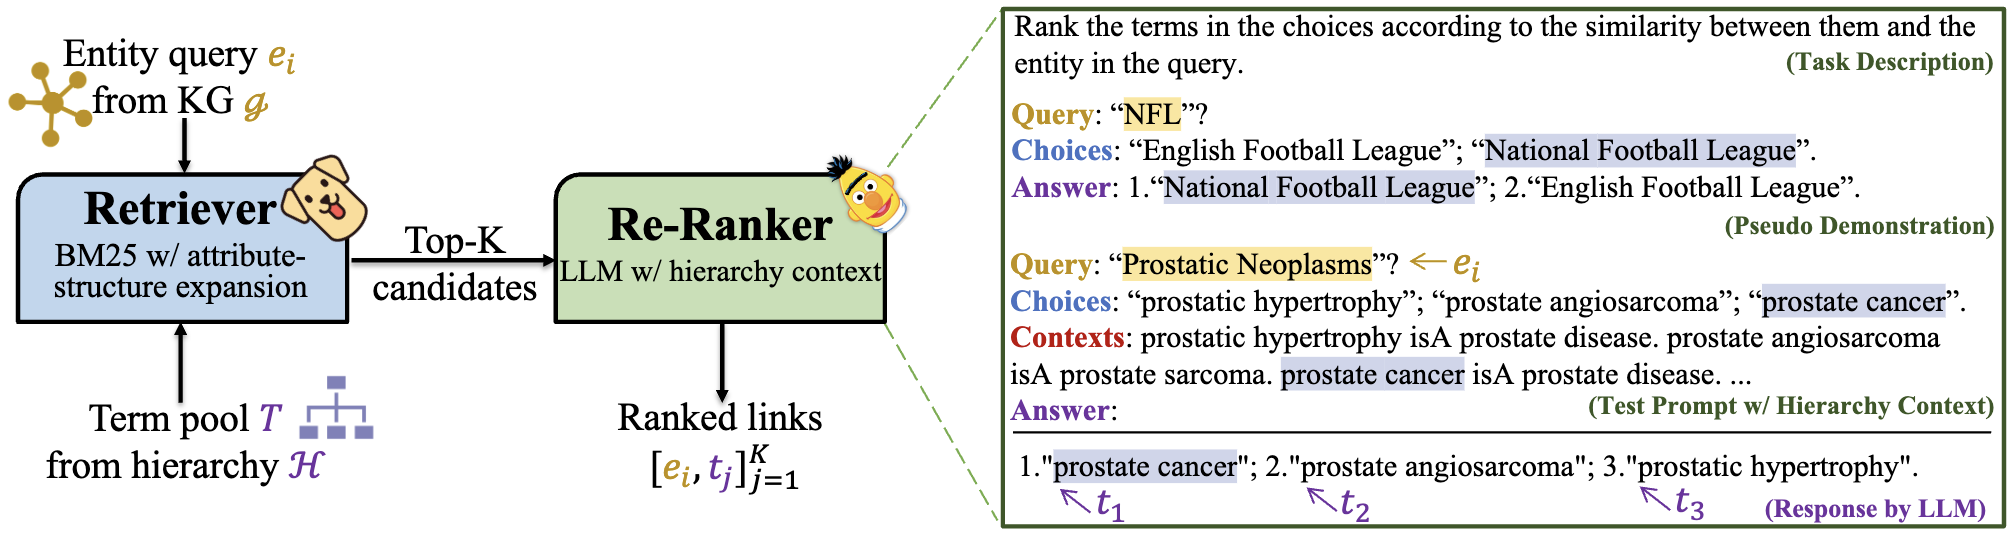
\includegraphics[width=.95\columnwidth]{submissions/CarlYang2024/figures/hiprompt.png}
    \end{center}
    \vspace{-4mm}
    \caption{The overall framework of Hiprompt.}
    \label{fig:hiprompt}
     \vspace{-2mm}
\end{figure}

Recent work has demonstrated the effectiveness of LLM-based approaches in KG integration. 
For example, Lu et al.~\citep{lu2023hiprompt} developed HiPrompt (framework shown in Figure~\ref{fig:hiprompt}), which aligns entities between biomedical KGs and standardized hierarchical entity taxonomies. 
This task poses significant challenges due to the scarcity of available pairs and the inconsistent naming conventions between KGs and entity taxonomies.
Their two-stage approach combines traditional information retrieval techniques (BM25) with LLM-based re-ranking using hierarchy-oriented prompts, achieving superior performance in few-shot biomedical knowledge-graph integration.  
Building on this direction, Xie et al.~\citep{xie2024promptlink} developed PromptLink, a framework that leverages both domain-specific language models and GPT-4 for cross-source biomedical concept linking. The framework employs a two-stage prompting mechanism by first eliciting the biomedical prior knowledge from the LLM for the concept linking task and then enforcing the LLM to reflect on its own predictions to further enhance their reliability. 
PromptLink’s success in zero-shot scenarios illustrates the potential of LLMs to generalize across diverse data sources without extensive training data.

In contrast to the two LLM approaches that primarily use LLMs for ranking candidate sets, AutoAlign \cite{zhang2023autoalign} employs off-the-shelf LLMs to construct a predicate-proximity graph that captures relationships between entity types rather than individual entities. It then aligns the entity embeddings of two KGs into a common vector space by calculating similarity based on entity attributes.


These advances suggest several promising future directions for LLM-aided KG integration. For example, LLMs could potentially facilitate the continuous integration of new knowledge into existing KGs dynamically and automatically by identifying and resolving conflicts between new and existing information, while maintaining consistency across the integrated knowledge base. Such real-time data integration is especially beneficial for dynamic applications like live event monitoring and real-world decision-making. {Furthermore, integrating KGs with LLMs remains challenging due to the risk of generating false or untrustworthy information~\cite{yang2024give}. To mitigate this issue, there is a growing need for improved human-in-the-loop systems. Specifically, enhanced interfaces~\cite{hassan2017claimbuster,nakov2021automated} can enable experts to more effectively verify and interpret LLM-generated recommendations, ensuring greater reliability and transparency.}



% Lu et al.~\citep{lu2023hiprompt} propose HiPrompt, an innovative framework that leverages LLMs for biomedical knowledge fusion. Their work addresses the challenge of aligning entities from biomedical KGs with terms in a standardized hierarchical index system, a task that traditionally suffers from scarce labeled data and inconsistent naming conventions. HiPrompt employs a two-stage approach: a retrieval module using BM25 with expanded entity and term representations, followed by an LLM-based re-ranking module that utilizes hierarchy-oriented prompts. This approach enables effective few-shot learning, outperforming both conventional unsupervised methods and neural embedding models in zero-shot and one-shot settings. It demonstrates the potential of LLMs in capturing complex semantic relationships and hierarchical constraints in KG integration tasks, even with minimal supervision. Their findings suggest that LLM-aided approaches could significantly advance the field of KG construction and integration, particularly in domains with limited labeled data.

% Another notable example is PromptLink~\citep{xie2024promptlink}, which leverages LLMs for cross-source biomedical concept linking. PromptLink combines the strengths of biomedical-specialized pre-trained language models and GPT-4 to address the challenges of inconsistent naming conventions across different data sources. The framework employs a two-stage prompting mechanism that efficiently filters candidates and generates reliable linking predictions, including NIL predictions when no suitable match is found. By outperforming conventional string-matching and machine learning-based methods in zero-shot accuracy, PromptLink demonstrates the potential of LLMs in enhancing KG integration tasks. This approach is particularly valuable in domains where labeled data is scarce and the ability to generalize across various data sources is crucial.

\subsection{Constructing and Completing KGs}
KGs have high-standard requirements on the quality of knowledge, regarding accuracy, consistency, coverage and freshness. No matter constructed through manual curation, NLP tools, or their combinations, KGs can unavoidably include erroneous knowledge. Moreover, when multiple KGs are integrated, conflicting knowledge can emerge. Finally, new knowledge is constantly generated from new experiments and research, making existing knowledge inaccurate and incomplete. LLMs have emerged as a promising solution, leveraging the vast and adaptable knowledge acquired during pre-training to overcome these limitations \cite{petroni2019language, yu2024kola, xu2024clingen, alkhamissi2022review}. 
The key advantage of LLMs for KG construction and completion is their ability to generate novel, semantically coherent information with minimal reliance on additional labeled data.

% The key advantage of LLMs in this domain lies in their ability to generate novel, semantically coherent information that can supplement and enrich existing KGs. Unlike rule-based or supervised machine learning approaches, LLMs can leverage their extensive understanding of language and the world to infer missing connections, identify new entities, and uncover implicit relationships - all without being constrained by the limitations of manually curated training data.

Recent studies have highlighted the effectiveness of LLM-based approaches for KG construction and completion. Zhu et al. \citep{zhu2023llms} utilize in-context learning capabilities of LLMs to complete tuples with missing entities or relations to generate new knowledge triplets for augmenting existing KGs.
Wei et al. \citep{wei-etal-2023-kicgpt} and Wang et al. \citep{wang-etal-2024-kc} tackle KG completion as a candidate identification and ranking task, proposing a “retrieve-rank” pipeline where LLMs are used to rerank top-retrieved entities, thus creating additional knowledge triplets.

An alternative approach to prompting LLMs involves using code-based prompts,  rather than natural language, to incorporate new entities into existing KGs~\cite{bi2024codekgc,zeng2024codetaxo}. 
Code LLMs, extensively trained on structured data such as programming code, are inherently well-suited to the structured nature of KGs.
Using a code-based interface enables more effective handling of graph-like structures, logical relationships, and precise reasoning~\cite{madaan2022language,chen2023program,shi2024agent}.
Specifically, Bi et al. \cite{bi2024codekgc} first encoded the schema of KGs by modeling code definitions, to capture the structural information inherent in the data. They then employed chain-of-thought prompting to produce accurate knowledge triples. This methodology demonstrates improved performance over traditional natural language-based prompts. 
Similarly, Zeng et al.~\citep{zeng2024codetaxo} proposed CodeTaxo, which represents entities within a base 'Entity' class, mirroring hierarchical relationships in programming constructs. This approach enables LLMs to efficiently create taxonomic structures by leveraging syntactic capabilities commonly used in code tasks, thus enhancing the organization and completeness of KGs. 
% Another notable example is CodeTaxo~\citep{zeng2024codetaxo} which encapsulates entities in a base class 'Entity' to better characterize hierarchical relations similar to programming constructs. This enables the LLM to efficiently process and generate taxonomic structures by leveraging its strong syntactic capabilities, which are typically associated with code understanding tasks. By combining the LLM's natural language understanding with its code-related skills, CodeTaxo demonstrates the versatility of these models in enhancing the completeness and organization of KGs.


The above methods primarily focus on prompting LLMs for KG construction and completion. While these methods show promise, they fall short in fully adapting LLMs to target tasks and can suffer from hallucination issues. To address these limitations, several studies aim to improve the quality of LLM-generated content for KG tasks. 
{Zhang et al. \cite{zhang2024extract} presented a three-phase framework for constructing KGs with LLMs to enhance contextual understanding and schema alignment. 
It starts with open information extraction to identify relation triplets from unlabeled textual corpora, followed by schema definition where LLMs generate contextually relevant descriptions for schema components. 
Finally, the extracted triplets are aligned with the schema.  
To further enhance the quality of the extracted
triplets and minimize the risk of misinformation, a schema retriever is used to generate a list of candidate entities and relations to guide the triplet extraction steps. This approach works for both predefined schemas and situations where the schema needs to be inferred from the context.
}
% \cite{zhang2024extract} presents a three-phase framework for constructing KGs with LLMs to enhance contextual understanding and schema alignment. The process begins with open information extraction, where relational triplets are identified from unlabeled textual corpora. Next, LLMs is used to define schema components by generating contextually relevant, human-like descriptions. In the final canonicalization phase, extracted triplets are aligned with the schema to ensure consistency and reduce redundancy. This adaptable framework is effective in both predefined schema settings and scenarios where schema must be inferred from context.
Additionally, various studies explored fine-tuning LLMs specifically for KG completion. Zhang et al.~\cite{kopa} proposed KOPA that first applies structural pre-training to create embeddings of entities and relations in KGs, and project embeddings into the textual space as virtual knowledge tokens. These tokens act as prefixes in LLM input prompts, enabling structure-aware reasoning that leverages both the generative power of LLMs and the retrieval of structured KG information to improve the accuracy and completeness of KG completion tasks. 
Jiang et al.~\citep{jiang2024kg} introduced KG-FIT for using open-world knowledge from LLMs to enhance KG embeddings. It initially constructs a semantically coherent, hierarchical structure of entity clusters, guided by LLM-powered entity representations. It then fine-tunes these embeddings by integrating the hierarchical structure with textual embeddings. This hybrid approach allows KG-FIT to capture both the semantic depth of LLMs and the structural information intrinsic to KGs, resulting in more comprehensive KG representations.



% TaxoPrompt~\citep{xu2022taxoprompt}, a prompt-based method for self-supervised taxonomy expansion that effectively leverages the global structure of taxonomies. TaxoPrompt integrates the taxonomic context into the training of a language model (LM) by employing a customized random walk algorithm that captures relational paths within the taxonomy. This context is then used in a prompt-tuning framework to transform the taxonomy expansion problem into a hypernym generation task. During the process, a template creates a cloze task where the LM predicts missing hypernyms based on provided context, thus maintaining the structural integrity of the taxonomy.


% https://arxiv.org/abs/2405.16412
% https://dl.acm.org/doi/pdf/10.1145/3637528.3671469
% https://arxiv.org/pdf/2408.09070
% https://www.ijcai.org/proceedings/2022/0615.pdf

\begin{figure}[htbp]
    \begin{center}
    %\framebox[4.0in]{$\;$}
    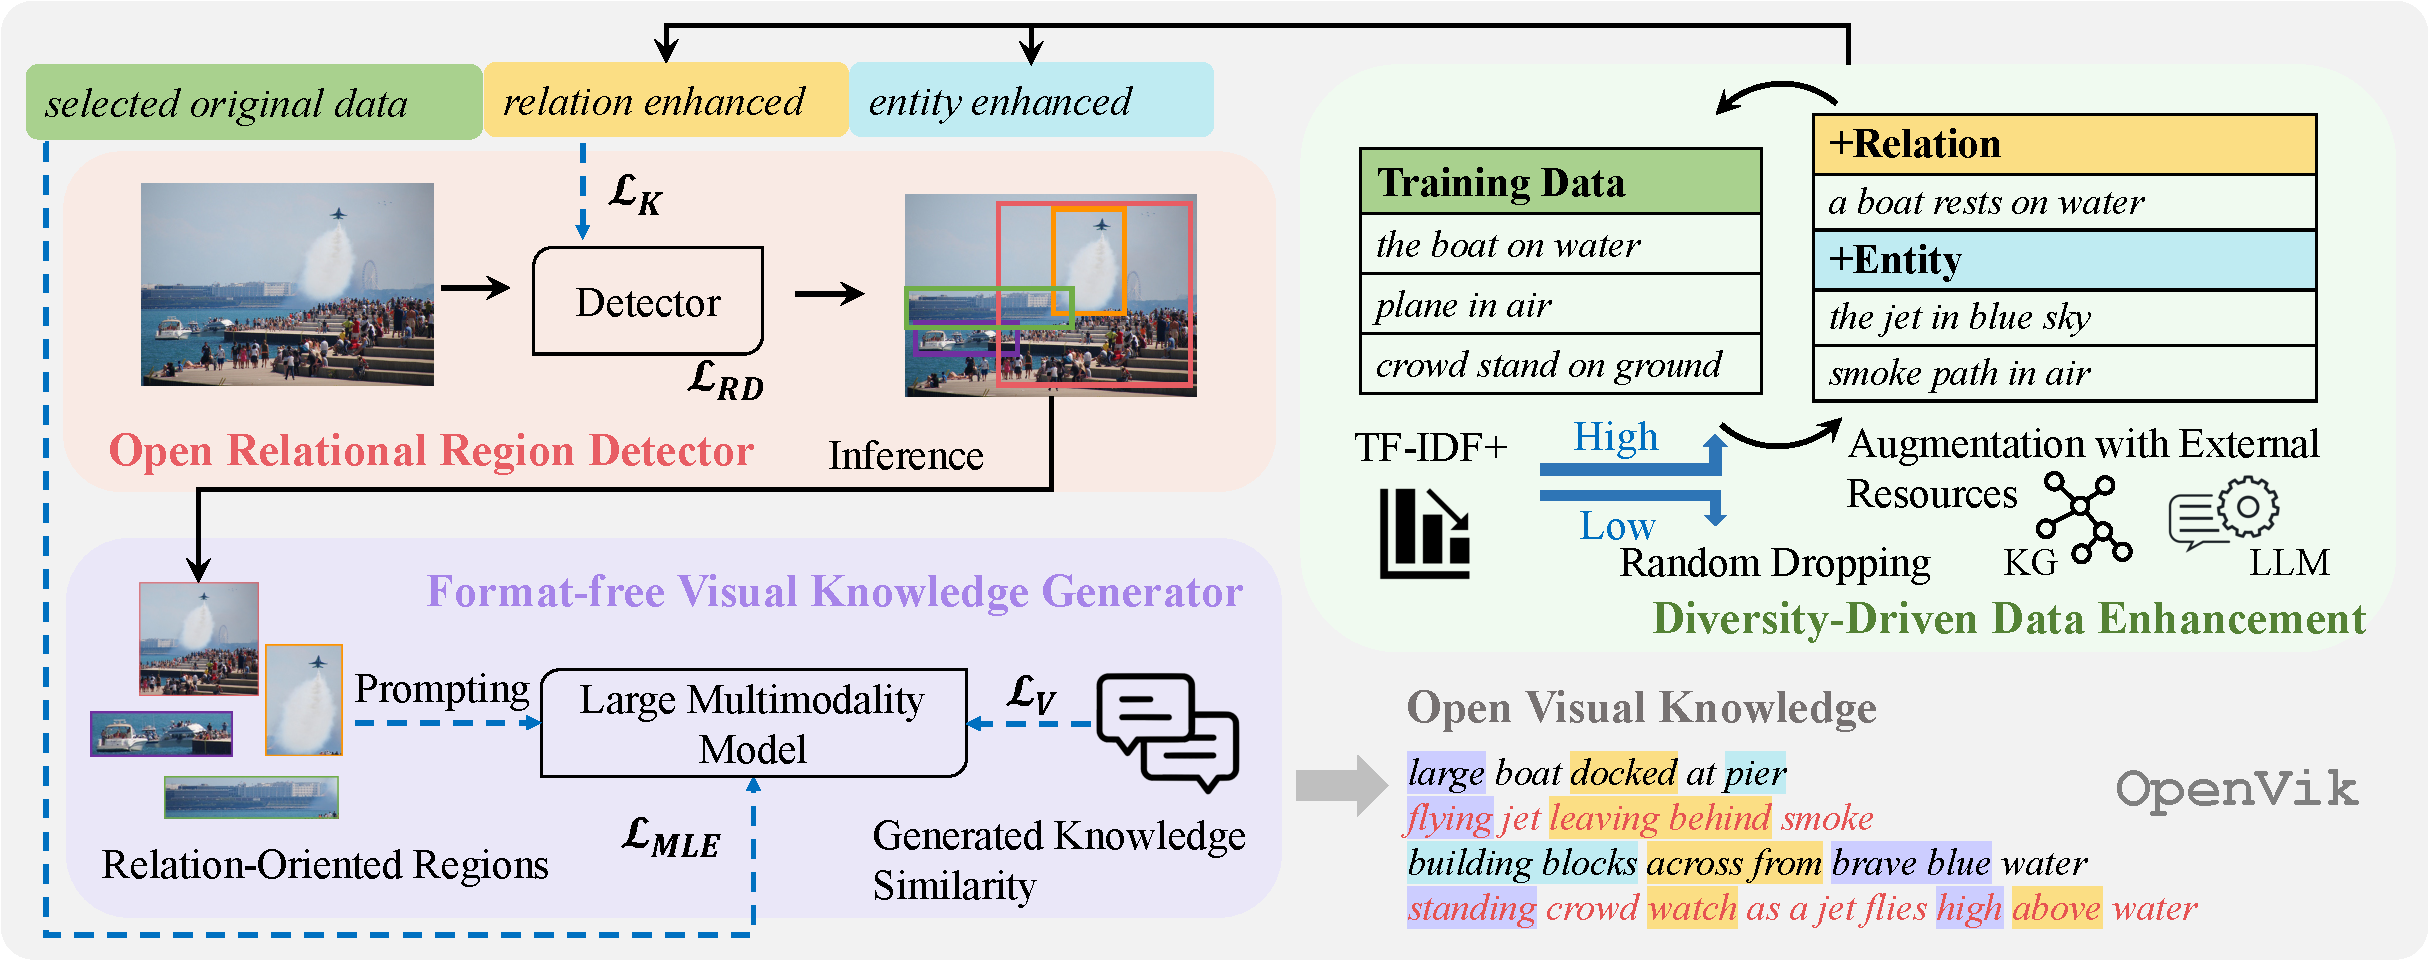
\includegraphics[width=.95\columnwidth]{submissions/CarlYang2024/figures/openvik.pdf}
    \end{center}
    % \vspace{-3mm}
    \caption{{The overall framework of OpenVik consists of two main components: (1) an open relational region detector, highlighted in the orange and purple panels, which includes a region regression loss ($\mathcal{L}_{\text{RD}}$) and a regional description loss ($\mathcal{L}_{\text{K}}$), and (2) a format-free visual knowledge generator, incorporating knowledge generation loss ($\mathcal{L}_{\text{MLE}}$) and diversity regularization ($\mathcal{L}_{\text{V}}$). These modules work collaboratively to extract open visual knowledge, incorporating novel entities and diverse relations in a format-free manner.}}
    \label{fig:openvik}
    % \vspace{-5mm}
\end{figure}



\subsection{Enriching KGs with multi-modality data}
Traditionally, specialized models and algorithms have been developed to process and analyze various modalities of data such as tables, texts, images, and time series. These methods can hardly perform integrative analysis across data modalities and generalize across different data platforms. Recently, LLM-based multi-modality foundation models (MMFMs) have shown strong promise in analyzing multi-modality data through the unified interface of languages \cite{yang2023dawn, fei2022towards, li2024multimodal, li2024llava, zhang2023biomedgpt}.
Integrating multi-modal data into KGs creates a more comprehensive representation of entities and their relationships, enhancing performance in open-world applications like image classification and visual question answering \cite{chen2024knowledge}. Many studies focus on using MMFMs for specific tasks, such as entity extraction \cite{sun2024umie,li2023prompting,hu2023prompt}, relation extraction \cite{yu2023visually,li2024zero,li2024pixels}, or event extraction \cite{chen2024schema,rasheed2024glamm}. However, these works often isolate extraction tasks without unifying entities and relations into a structured KG.
{A pioneering approach in this direction is OpenVik \cite{cui2024open} (framework shown in Figure~\ref{fig:openvik}). It first trains an open relational region detector to locate image regions containing relational information. 
It then employs a visual knowledge generator to create format-free knowledge descriptions by prompting a large visual language model. Through the use of MMFM, OpenVik advances KG completion by integrating rich visual context, expanding knowledge coverage, and enhancing the accuracy of representation within the resulting KG.}
Application-wise, Yang et al.~\cite{yang2024hierarchical}  proposed an automated approach to constructing product KGs from raw images in e-commerce. This method first employs vision-language models (VLMs) to extract detailed image information and then uses an LLM to reason and infer additional KG properties not visually present, hierarchically expanding, and linking nodes to develop comprehensive, scalable KGs without human input.


% https://www.cs.emory.edu/~jyang71/files/openvik.pdf
\newcommand{\gG}{\mathcal{G}\xspace}
\newcommand{\gL}{\mathcal{L}\xspace}
\newcommand{\gZ}{\mathcal{Z}\xspace}

\section{KG-guided LLM Enhancement}
LLMs have shown impressive communication and question-answering capabilities, demonstrating strong promise in various applications \cite{wang2024survey, wu2023bloomberggpt, cui2023chatlaw, chen2023genept, singhal2023large, singhal2023towards, haupt2023ai, nori2023capabilities, lee2023benefits, fleming2023assessing, chen2023meditron, yang2022large, luo2022biogpt, agrawal2022large, mehandru2024evaluating, zhang2023biomedgpt, biswas2023role, dash2023evaluation}. 
%answering medical questions \cite{singhal2023large, singhal2023towards, haupt2023ai, nori2023capabilities, lee2023benefits, fleming2023assessing, chen2023meditron}, extracting clinical information \cite{yang2022large, luo2022biogpt, agrawal2022large} and assisting clinical decisions \cite{mehandru2024evaluating, zhang2023biomedgpt, biswas2023role, dash2023evaluation}. 
%However, LLMs are also shown to ``hallucinate'' false outputs and unsubstantiated answers \cite{hal, hal3, hal4}, preventing their adoption in diverse fields, especially those with high-standard requirements on the accuracy and factuality of responses such as healthcare \cite{hal7}. Recently, many technical frameworks have been proposed to detect or avoid hallucinations in LLMs, such as based on supervision for reinforcement learning \cite{hal8}, statistical uncertainty measurements \cite{hal} and \todo{xxx \cite{}}. 
However, to reliably model domain-specific data and generate factual and accurate answers, LLMs still face the challenges of lacking domain knowledge, fuzzy inferences, and hallucination \cite{hu2023large, mousavi2024your, yadkori2024believe, asai2024selfrag,yu2024rankrag, liu2023evaluating, zhu2023dyval, zhuo2024roles, yuan2024back, wang2023boosting, ji2023survey, bai2024hallucination, tonmoy2024comprehensive, maynez2020faithfulness, xiao2021hallucination, farquhar2024detecting, ji2023towards, chen2024inside}.
% \textit{lack of knowledge} \cite{hu2023large, mousavi2024your, xu2024kg, becker2024cycles, yadkori2024believe, kim2024m}, \textit{fuzzy inference} \cite{liu2023evaluating, zhu2023dyval, bai2024kgquiz, zhuo2024roles, baek2024researchagent, yuan2024back, wang2023boosting}, and \textit{hallucination} \cite{ji2023survey, bai2024hallucination, tonmoy2024comprehensive, maynez2020faithfulness, xiao2021hallucination, farquhar2024detecting, ji2023towards, chen2024inside}
Retrieval augmented generation (RAG) \cite{lewis2020retrieval}, which aims at retrieving query-relevant evidence and generating evidence-based answers, has strong promise in evidence-critical domains. However, effective and efficient RAG for complex queries is still challenging which requires LLMs to be able to (1) generate logical plans for retrieving multiple pieces of relevant evidence from complex data, (2) conduct valid reasoning and inference to compose the pieces of evidence towards generating coherent answers, and (3) reliably guarantee the detection and removal of errors. In the following, we discuss how these challenges can be addressed with well-designed planning, reasoning, and reflection frameworks with the help of KGs.

{
\newcommand{\ourmethod}{\texttt{RoG}\xspace}
\subsection{Planning with domain knowledge}
% \carl{Linhao, the current 3.1 is too long-- we aim to write about 12 pages of main contents in total and the plan is to write about 2 (front page/intro)+ 3 (sec 2) + 3 (sec 3) + 2 (sec 4) + 1 (sec 5) + unlimited references. Can you perhaps try to separate the current contents into 3.1 (planning) and 3.2 (reasoning)? Please try to re-organize/re-write the contents more so they also read differently from your RoG paper. Please also add some discussions about more related recent works separately in both subsections. I added a reference in 3.3, but please let me know if you are not sure about what to write in 3.3. Thanks!}\\
While LLMs excel in many NLP tasks \cite{brown2020language,bang2023multitask}, they still face challenges in acquiring domain knowledge. To address this issue, many attempts seek assistance from KGs, which are often constructed to represent knowledge in specific domains, such as medicine \cite{bodenreider2004unified}, law \cite{kang2024bridging}, and finance \cite{liu2019anticipating}. The integration of KGs and LLMs has shown promising results in various applications, such as question answering \cite{jiang2023unikgqa}, recommendation \cite{wang2023enhancing}, and dialogue systems \cite{tuan2022towards}. Despite the success, there are still challenges in effectively obtaining useful information from KGs and incorporating them into LLMs. 

Existing methods typically depend on a retriever to obtain relevant triples. For example, Baek et al. \cite{baek2023direct} proposed a direct retrieval method to retrieve relevant triples from KGs. However, the retriever may not always retrieve the most relevant triples, leading to suboptimal performance. Additionally, KGs contain a wealth of domain-specific knowledge, making it challenging for LLMs with limited domain expertise to comprehend and utilize this information. To further unleash LLMs' capabilities of leveraging domain knowledge, the \textit{plan-and-solve} paradigm \cite{wang2023plan} has been proposed, in which LLMs are prompted to first generate a plan. Based on the plan, LLMs can retrieve the relevant domain knowledge and conduct reasoning to generate answers \cite{yaoreact}. However, existing methods are incapable of handling the complex structured knowledge in KGs to enable effective planning and reasoning. To address this issue, we propose a \textit{planning-retrieval-reasoning} framework named \ourmethod that enables LLMs to plan and reason on KGs \cite{luo2024reasoning}. The overall framework is illustrated in \Cref{fig:rog}.

\begin{figure}[htbp]
    \begin{center}
    %\framebox[4.0in]{$\;$}
    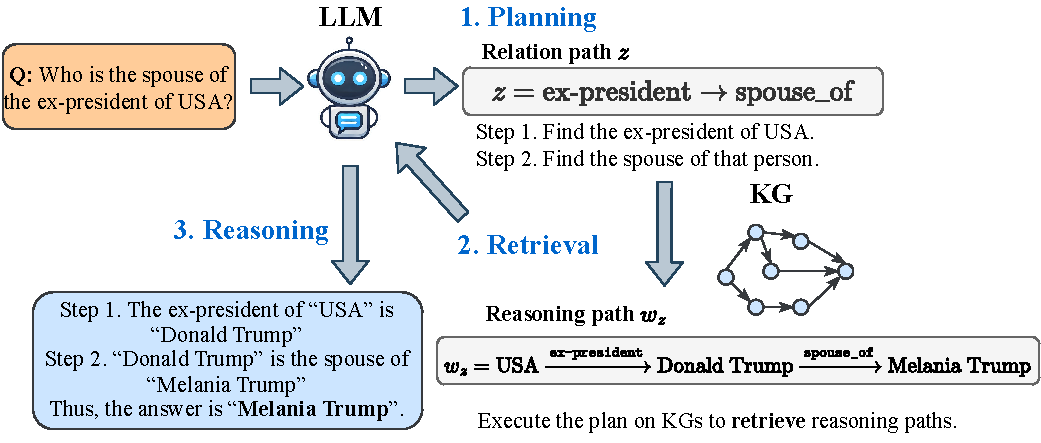
\includegraphics[width=.85\columnwidth]{submissions/CarlYang2024/figures/rog.pdf}
    \end{center}
    % \vspace{-3mm}
    \caption{The overall framework of planning and reasoning on KGs (\ourmethod).}
    \label{fig:rog}
    % \vspace{-5mm}
\end{figure}

\ourmethod first generates several relation paths that are grounded by KGs as plans. Relation paths, which capture semantic relations between entities, have been utilized in many reasoning tasks on KGs \cite{wang2021relational,xusubgraph}. Based on relation paths, we can always retrieve the latest knowledge from KGs with a simple constrained breadth-first search. Therefore, relation paths can serve as faithful plans to guide the retrieval and reasoning on domain-specific KGs. Additionally, by treating relation paths as plans, we can make sure the plans are grounded by KGs, which enables LLMs to retrieve relevant knowledge and conduct faithful reasoning. To this end, we formulate our \ourmethod as an optimization problem that aims to maximize the probability of reasoning the answer from a KG $\gG$ w.r.t the question $q$ by generating relation paths $z$ as the plan:
\begin{equation}
    % \setlength\abovedisplayskip{1pt}%shrink space
    % \setlength\belowdisplayskip{1pt}
    \label{eq:plan}
    P_\theta(a|q,\gG) = \sum_{z\in\gZ}P_\theta(a|q,z,\gG)P_\theta(z|q),
\end{equation}
where $\theta$ denotes the parameters of LLMs {and $a$ denotes the final answer.} To enable accurate planning with domain knowledge, we design two instruction tuning tasks: 1) \textit{planning optimization}, which distills the knowledge from KGs into LLMs to generate faithful relation paths as plans; 2) \textit{retrieval-reasoning optimization}, which enables LLMs to reason based on the retrieved reasoning paths.
{
The final objective function of \ourmethod is the combination of the planning optimization and retrieval-reasoning optimization, which can be formulated as
\begin{equation}
    \setlength\abovedisplayskip{1pt}%shrink space
    \setlength\belowdisplayskip{1pt}
    \label{eq:final_obj}
    \gL = \log \underbrace{P_\theta(a|q,\gZ^*_K,\gG)}_{\text{Retrieval-reasoning}} + \underbrace{\frac{1}{|\gZ^*|}\sum_{z\in Z^*}\log P_\theta(z|q)}_{\text{Planning}},
\end{equation}
where we use the shortest paths $\gZ^*\subseteq\mathcal{Z}$ between $q$ and $a$ in KGs as supervision signals. We maximize the probability of LLMs generating faithful relation paths through distilling the knowledge from KGs.
}
In this way, with the proposed \ourmethod, LLMs can effectively retrieve domain knowledge from KGs with planning, which significantly enhances the reasoning capability of LLMs.
}

{
    \newcommand{\ourmethod}{\texttt{GCR}\xspace}
\subsection{Reasoning with structured knowledge}
% https://arxiv.org/abs/2410.13080
KGs capture abundant factual knowledge in a structured format, which provides a faithful knowledge source for improving the reasoning abilities of LLMs \cite{pan2024unifying}. Nevertheless, because of the unstructured nature of LLMs, directly applying them to reason on structured KGs is challenging. Early works focus on fine-tuning LLMs together with structured knowledge from KGs to enrich the knowledge of LLMs for better reasoning \cite{zhang2019ernie,rosset2020knowledge}. For example, KEPLER~\cite{wang2021kepler} directly employs both KG embedding training objective and Masked token pre-training objective into a shared transformer-based encoder. Through fine-tuning, LLMs can better understand the structured knowledge in KGs for reasoning. However, the fine-tuning process is computationally expensive and incapable of efficiently adapting to the evolving real-world knowledge. 

Recently, researchers have combined the strengths of retrieval-based methods with the prompting technique to enable LLMs to reason on KGs \cite{lewis2020retrieval,jiang2023unikgqa}. CoK \cite{wang2023boosting} and KD-CoT \cite{wang2023knowledge} retrieve facts from an external KG to guide the CoT performed by LLMs. To capture graph structure, GNN-RAG \cite{mavromatis2024gnn} adopts a lightweight graph neural network to effectively retrieve knowledge from KGs, which are formatted as a sentence path to elicit the reasoning process of LLMs. Mindmap \cite{wen2023mindmap} builds a prompt-based method that endows LLMs with the capability of comprehending KG and reasoning with it. Despite the success of these methods, they still face challenges in designing principled prompts to represent KGs and conduct reasoning. Moreover, LLMs still have limited capabilities in understanding the graph structure and reasoning with the text-based graph prompts \cite{huang2024can}. 

Different from existing efforts that require a computationally expensive fine-tuning phase or design ad-hot prompts for LLMs,  we recently introduced a KG-constrained reasoning (\ourmethod) paradigm \cite{luo2024graph}. \ourmethod connects unstructured reasoning in LLMs with structured knowledge in KGs, seeking to achieve efficient and effective reasoning on structured knowledge. The overall framework is illustrated in \Cref{fig:gcr}.

\begin{figure}[htbp]
    \begin{center}
    %\framebox[4.0in]{$\;$}
    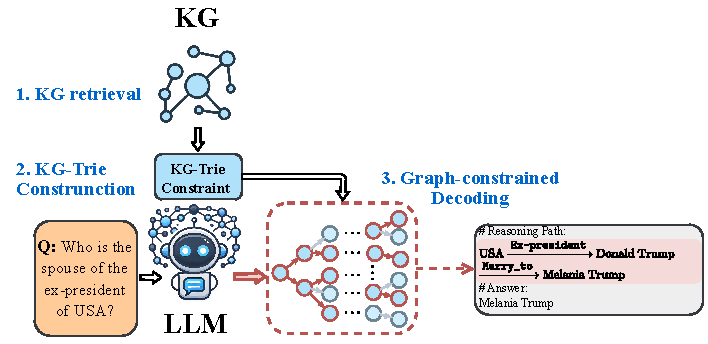
\includegraphics[width=.75\columnwidth]{submissions/CarlYang2024/figures/gcr.pdf}
    \end{center}
    % \vspace{-3mm}
    \caption{The overall framework of KG-constrained reasoning (\ourmethod).}
    \label{fig:gcr}
    % \vspace{-5mm}
\end{figure}

Graph-constrained reasoning, inspired by the concept that LLMs reason through decoding \citep{wei2022chain}, incorporates the KG structure into the LLM decoding process. This enables LLMs to directly reason on graphs by generating reliable reasoning paths grounded in KGs that lead to correct answers. Specifically, given a question, we first adopt a retrieval module to find a relevant KG that is helpful for reasoning. Then, we convert the KG into a structured index, KG-Trie, to facilitate efficient reasoning on KG using LLMs. Trie is also known as the prefix tree \citep{fredkin1960trie} that compresses a set of strings, which can be used to restrict LLM output tokens to those starting with valid prefixes. KG-Trie encodes the reasoning paths in KGs as formatted strings to constrain the decoding process of LLMs. Then, we propose graph-constrained decoding that employs a lightweight KG-specialized LLM to generate multiple KG-grounded reasoning paths and answers. With the constraints from KG-Trie, we ensure faithful reasoning while leveraging the strong reasoning capabilities of LLMs to efficiently explore paths on KGs in constant time. In this way, \ourmethod bridges the gap between structured knowledge in KGs and unstructured reasoning in LLMs, allowing for efficient reasoning on KGs via LLM decoding.

}
\subsection{Reflecting with atomic knowledge}
% \carl{https://arxiv.org/abs/2311.13314}\\
% https://arxiv.org/pdf/2310.11638\\
% https://arxiv.org/pdf/2402.11199\\
LLMs have shown impressive capabilities in encapsulating massive knowledge and conducting reasoning. However, they still face challenges in generating factually correct and faithful responses, especially in the presence of hallucinations \cite{huang2023survey}. KGs store atomic knowledge in a structured format, which can be used to verify the correctness of generated responses and detect hallucinations \cite{agrawal2023can}. To incorporate the factual knowledge from KGs into LLM hallucination detection, Guan et al. \cite{guan2024mitigating} proposed a retrieval-based method called KG-based retrofitting (KGR). KGR retrieves relevant facts from KGs during the LLM reasoning process, which are used to mitigate factual hallucination by retrofitting the initial responses. KGR enables an autonomous knowledge verifying and refining procedure with the factual knowledge retrieved from KGs, which significantly improves the reliability of LLMs. 

The hallucination of LLMs is usually attributed to the lack of factual knowledge of LLMs. To systematically evaluate the factual knowledge inside LLMs, as shown in \Cref{fig:reflecting}a, we propose a novel framework to automatically assess the factual knowledge in LLMs by using KGs \cite{luo2023systematic}. Unlike conventional methods that rely on human-annotated question-answering datasets, we systematically generate valid and diverse questions from KGs
with different difficulties while also ensuring knowledge coverage. Specifically, we retire the atomic knowledge from KGs as sets of triples. Then, we utilize different question generation methods, e.g., template-based and LLM-based methods, to convert the triples into question-answer pairs. The generated pairs are used to evaluate the factual knowledge of LLMs by comparing the generated answers with the ground-truth answers. The evaluation results can be used to reflect the factual knowledge of LLMs. In this way, we can systematically evaluate the factual knowledge of LLMs and provide insights into the hallucination behavior of LLMs, which can be used to improve the reliability of LLMs in various applications. 

Apart from the factual knowledge, the structure of KGs can be also utilized to justify the reasoning process of LLMs. Minh-Vuong et al \cite{nguyen-etal-2024-direct} designed a framework that delves deeper into the CoT reasoning capabilities of LLMs in multi-hop question answering by utilizing KGs, as shown in \Cref{fig:reflecting}b. The framework contains two evaluation modules: discriminative evaluation and generative evaluation. The discriminative evaluation aims to analyze whether the LLMs possess enough knowledge to conduct faithful reasoning. It feeds both valid and invalid reasoning paths retrieved from KGs into LLMs and asks them to predict the validity of these paths. The generative evaluation, on the other hand, aims to evaluate the faithfulness of the reasoning process of LLMs by grounding it on KGs. Given a reasoning process generated by LLMs, the generative evaluation module retrieves the facts from KGs, which are compared with the ground-truth reasoning paths. The evaluation results can be used to reflect the reasoning capabilities of LLMs and provide insights into the faithfulness of LLM reasoning. Based on the findings, although LLMs have shown impressive reasoning capabilities, they still face challenges in conducting faithful reasoning, especially in multi-hop question answering. 

\begin{figure}[htbp]
    \begin{center}
    %\framebox[4.0in]{$\;$}
    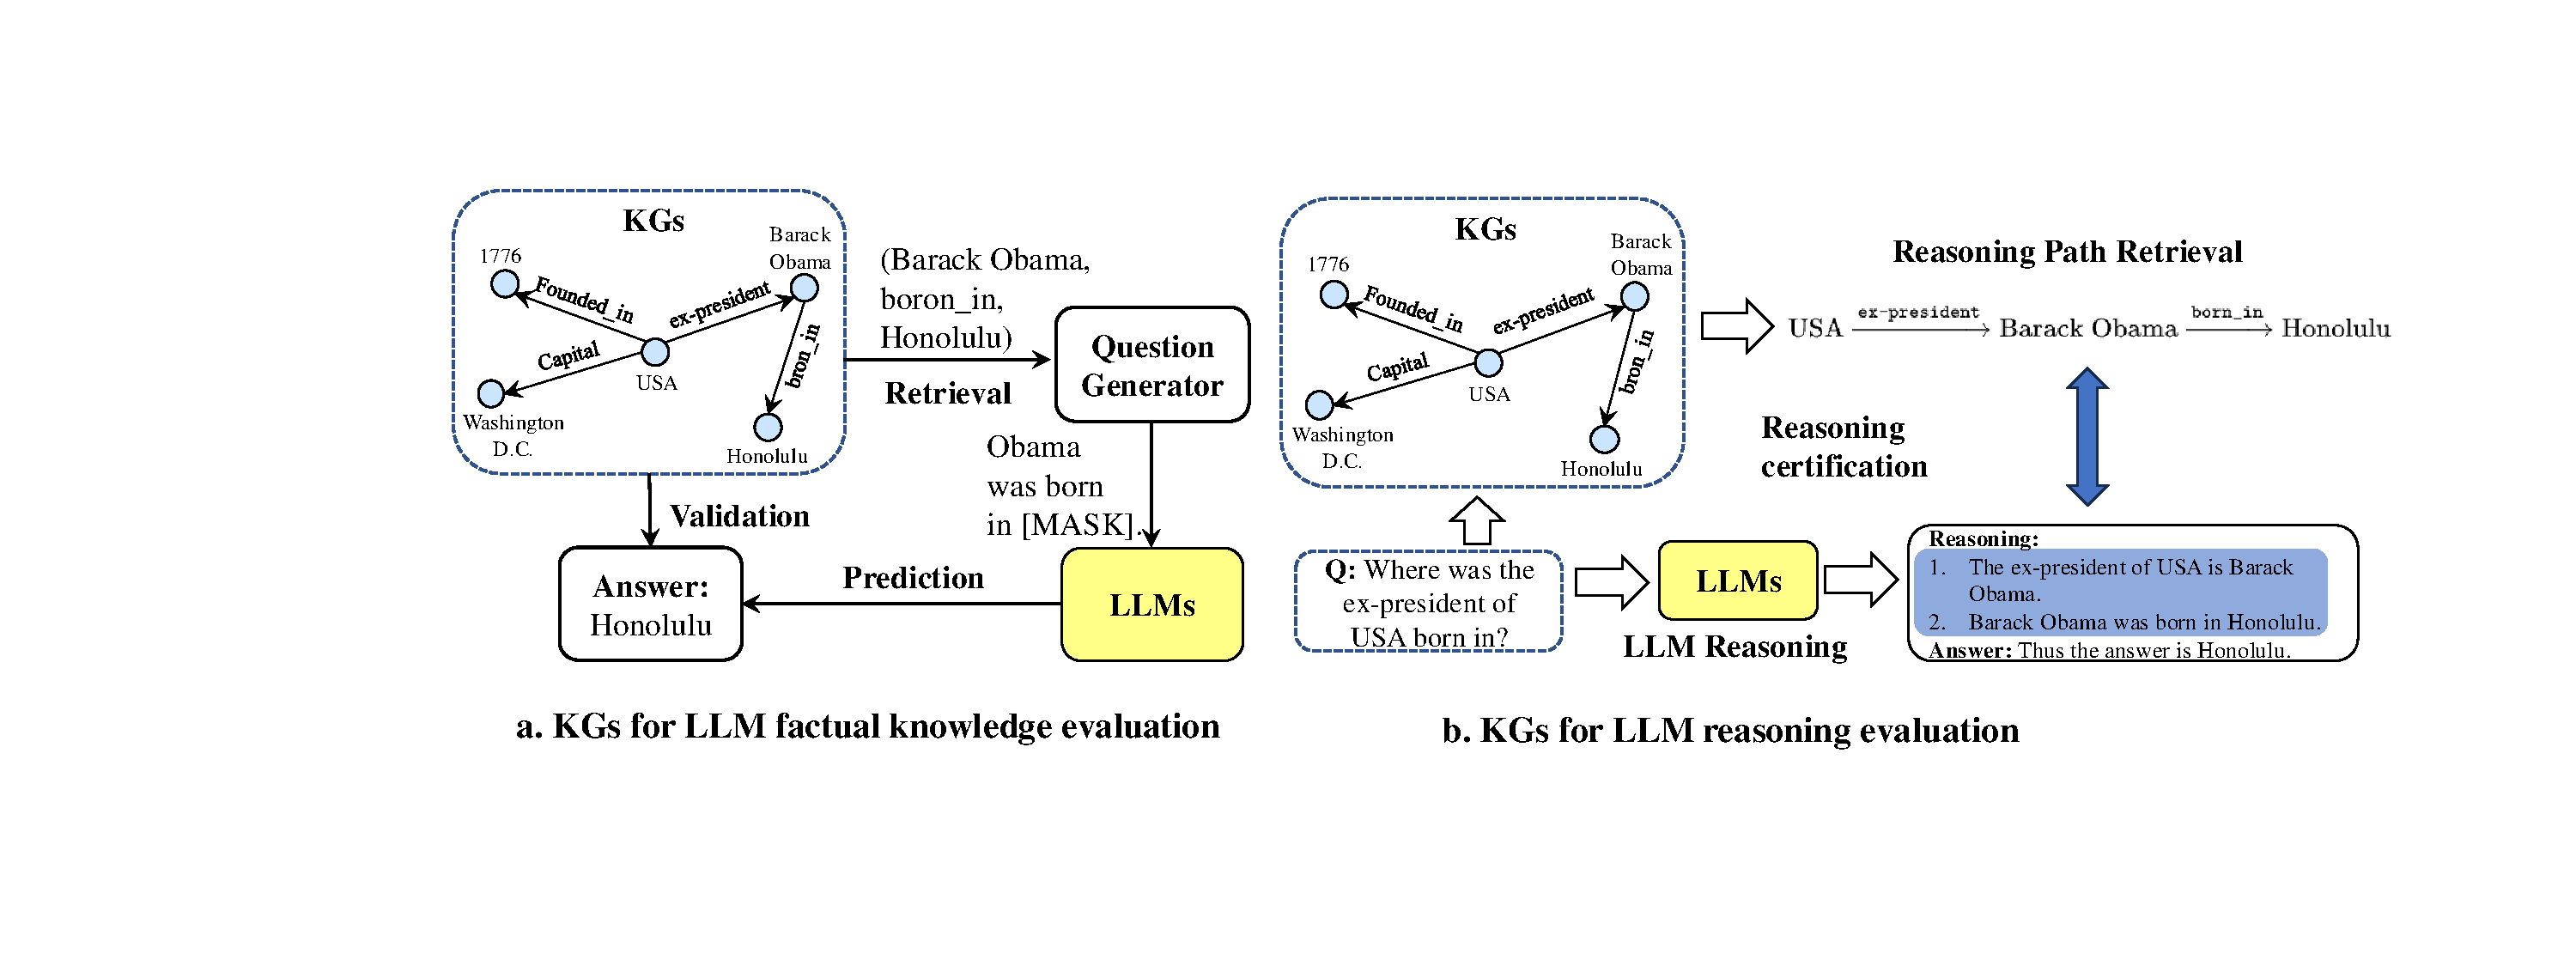
\includegraphics[width=1\columnwidth]{submissions/CarlYang2024/figures/reflecting.pdf}
    \end{center}
    % \vspace{-3mm}
    \caption{The illustration of LLM reflection with KGs. (a) The evaluation of the factual knowledge inside LLMs. (b) The evaluation of the reaosning process of LLMs with KGs.}
    \label{fig:reflecting}
    % \vspace{-5mm}
\end{figure}
\section{Knowledge-aware Multi-agent Federation}
%\carl{TODO: will work on this section over the weekend}\\
While KGs and LLMs can mutually enhance each other, data are properties and many real-world datasets are privately collected and owned by different institutions, which cannot be simply put together to train more powerful models. 
Moreover, many real-world applications require domain-specific knowledge that may not have been captured by general-purpose KGs and LLMs yet, and such knowledge can also be private properties. 
Finally, while the development of KGs and LLMs is highly automated and data-driven, the values and needs of different human stakeholders may not have been properly reflected in the data and models. 
Federated learning (FL) provides a robust and principled framework for privacy-protected multi-site collaboration, but proper implementation of FL in the new era of generative AI remains unclear; the further incorporation of domain knowledge and human participation is also highly under-explored. In the following, we will envision an innovative Federated Multi-Agent System (FedMAS) for multi-site privacy-protected, knowledge-infused, and human-engaged KG-LLM co-learning scenarios. 


Nowadays, while common practices in AI applications still largely resort to in-house development of models based on public and local data, the successes of generative AI, where complex models are trained with large-scale data, have demonstrated a strong need to collaboratively utilize local data towards obtaining powerful models that can generalize across institutions, finding and utilizing deep data patterns underlying common and rare use cases. Towards protecting local data privacy during collaborative model training, FL provides a promising solution \cite{nguyen2022federated, antunes2022federated, nguyen2022federated, antunes2022federated, xu2021federated, rieke2020future}. However, existing FL frameworks, by merely preventing the direct sharing of training data, are not effective in the scenarios of KG-LLM co-learning, because (1) as the construction of comprehensive KGs necessitates the incorporation of knowledge discovered from local data, private information may get reversely inferred from the collaboratively constructed KG; (2) as powerful generative models like LLMs can easily memorize training data, collaboratively trained LLMs may expose private information facing deliberately composed jailbreaking prompts \cite{wei2024jailbroken, wang2023decodingtrust, xu2024llm}.

In our pioneering studies on FL for graphs \cite{he2021fedgraphnn, xie2021federated, zhang2021subgraph, zhang2024deep, xie2023federated, zhang2022efficient, gu2023dynamic, xie2024federated}, we developed several novel algorithms for different graph separation scenarios. In FedDEP \cite{zhang2024deep}, we developed a prototype-based embedding sharing algorithm with local graph differential privacy (DP) guarantees, and demonstrated its utility in FL for global graph embedding models across private local subgraphs; in FedR \cite{zhang2022efficient}, we showed that sharing relation embeddings across local KGs can help FL for global KG embeddings with less privacy leakage. These studies have laid the foundations for our envisioned framework here, which will build on the private embedding sharing algorithms to construct \textit{multi-view KGs} that can facilitate multi-site knowledge sharing with minimum risks of exposing local private data.

\begin{figure}[htbp]
    \begin{center}
    %\framebox[4.0in]{$\;$}
    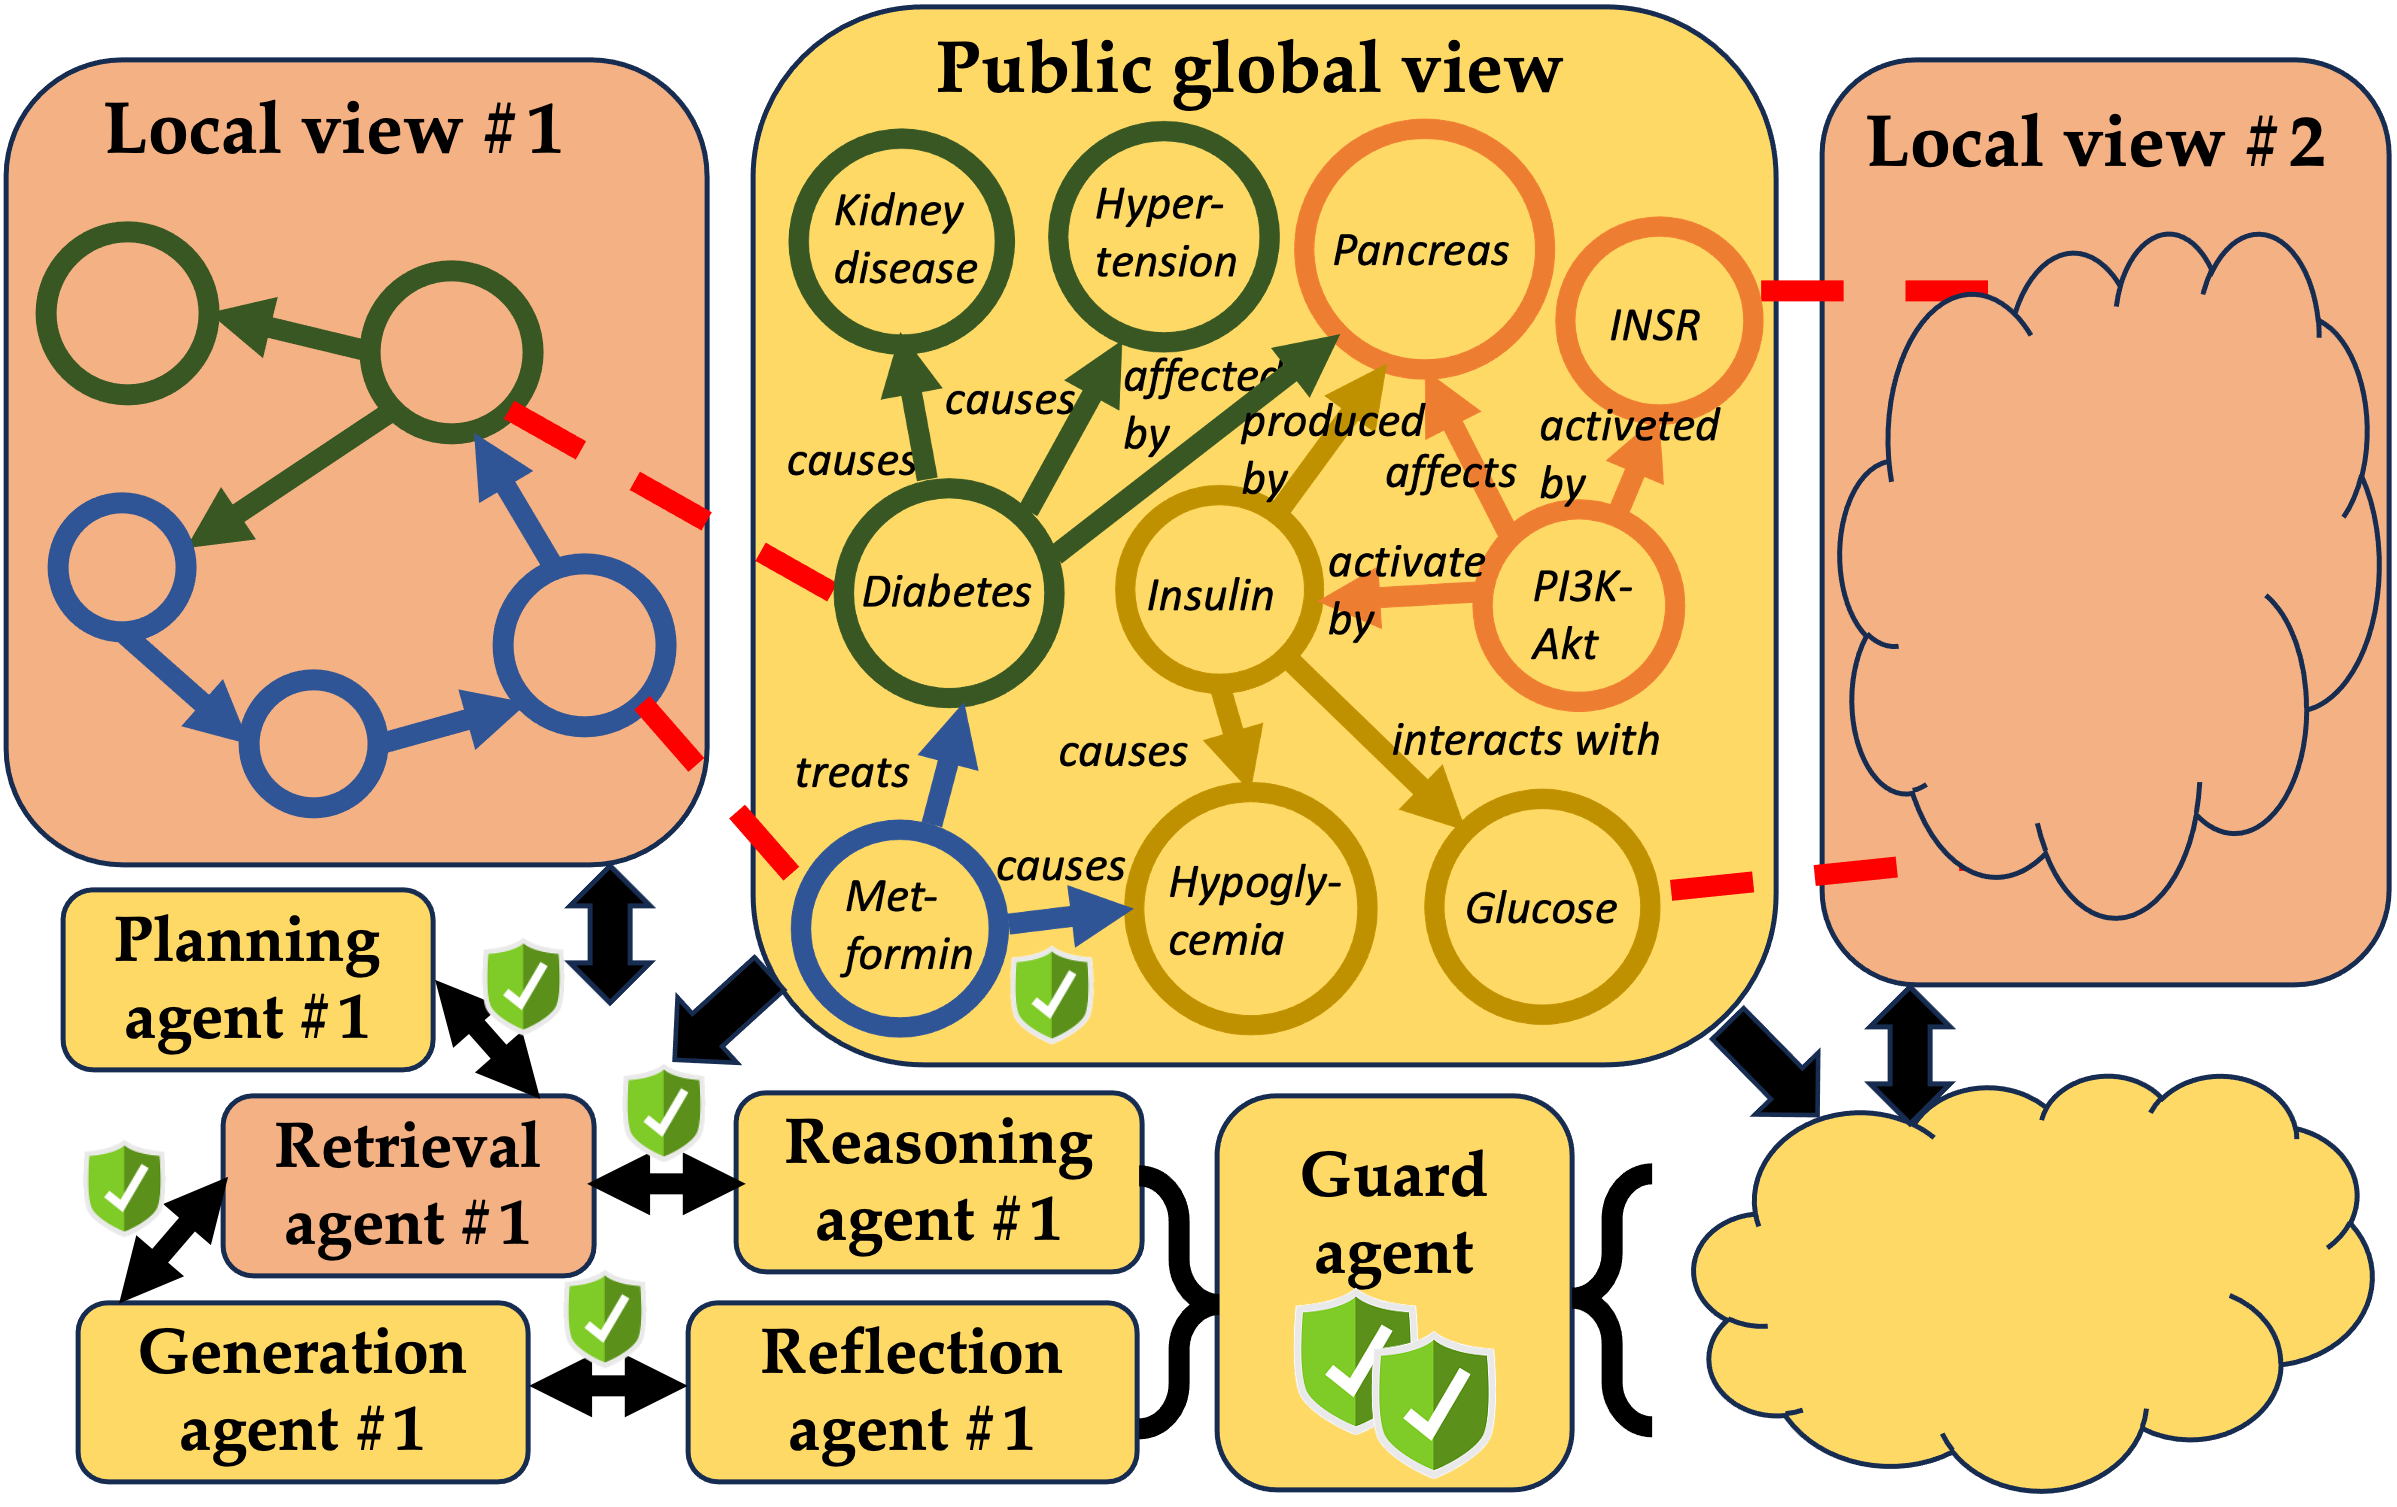
\includegraphics[width=.75\columnwidth]{submissions/CarlYang2024/figures/fedmas.png}
    \end{center}
    % \vspace{-3mm}
    \caption{The envisioned framework of a federated multi-agent system (FedMAS).}
    \label{fig:fedmas}
    % \vspace{-5mm}
\end{figure}

As illustrated in Figure \ref{fig:fedmas}, our envisioned FedMAS will include a multi-view KG and various LLM agents. The federation on KG will be implemented by collectively constructing a multi-view KG by all participating sites, where knowledge from public resources is integrated into the global view, and knowledge from private resources is kept in each site's local view only visible to itself. For each site, entities in its local view are linked with the global view, and only the embeddings related to these linked entities are shared with the server and other sites, via privacy-guaranteed embedding sharing algorithms such as those developed in FedDEP \cite{zhang2024deep} and FedR \cite{zhang2022efficient}. In this way, each local site can compute embeddings on its local view and the public view as if they can see all other sites' local views, allowing them to effectively adjust their local knowledge and further enhance their local LLMs, all without actually seeing the other sites' local views (knowledge). The server will periodically adjust knowledge in the global view also based on the shared privacy-guaranteed embeddings, and apply additional privacy checks to make sure no sensitive knowledge gets propagated into the global view.
%potentially discussing why knowledge is less private and how to avoid inference attack on embeddings

To rigorously protect the more sensitive patient data during the federation on LLM, it is possible to train multiple LLM agents in each site with different functions and let them collaborate through conversations instead of traditional model sharing, so the system can strictly control the level of private data each agent can access and monitor or moderate their collaborations. 
%Based on this design of multi-view KG, we will further enable the federation on LLM by training multiple LLM agents in each site and let them collaborate inside and across sites through conversations. 
%To control the levels of private data access and facilitate the moderation of conversations, each site will train multiple LLM agents focusing on different functions such as planning, retrieval, reasoning, reflection and answer generation. Since all agents will access certain levels of local private data during training and inference, none of them can be directly trained across sites even through FL. To this end, we will build on AutoGen \cite{} to design a structured conversational environment for multi-agent collaboration of LLMs. 
Specifically, since the retrieval agents need to access all local patient data, one plan is to implement programmable guardrails \cite{rebedea2023nemo} on its conversations with all other agents within the same site and forbid them from directly communicating with agents from other sites. Since all other agents can only access patient data indirectly through the retrieval agents, it is possible to adapt techniques such as our recently developed GuardAgent \cite{xiang2024guardagent} based on the clear goals and typical outputs of each agent to monitor all cross-site conversations, detecting and removing any suspicious private information.
%Specifically, since the retrieval and generation agents can directly access local patient data, we will only enable strict one-way conversations from other agents to them; since the planning, reasoning and reflection agents only access local KGs and their performances can likely benefit from cross-site collaborations (such as due to richer knowledge access and more generalized capabilities), we will enable two-way conversations among them cross sites; when the system is normal, we do not expect the agents to ask or answer privacy sensitive questions, and since each agent has clear goals, it will also be relatively easy to detect abnormal conversations; we will also explore techniques such as DP-prompting \cite{} to moderate the conversations against privacy leakage, and conduct red teaming \cite{} to rigorously monitor the conversations.  

When applying FedMAS to specific application domains such as finance, law, education, and healthcare, it is promising to leverage the knowledge-based data sharing mechanism to incorporate existing domain knowledge towards further alleviating knowledge gaps and mitigating potential biases. 
Built on recent promising results from LLM-based data annotations as discussed in Section 2, FedMAS can utilize specialized LLM agents to perform comprehensive extraction of structured knowledge from existing guidelines and tutorials and automatically integrate them with existing general and domain-specific KGs. For example, in healthcare, one type of important domain-specific entity is social determinants of health (SDOH) \cite{artiga2020disparities, artiga2018beyond, who2008closing}. The system can start with a set of known SDOH such as defined by WHO \cite{marmot2005social, phelan2010social}, and further extend the set and discover their impacts and relationships with various risk factors by investigating relevant healthcare literature. The KGs enhanced through these steps are supposed to facilitate the alleviation of various health disparities when utilized by subsequent LLM agents in the FedMAS. 
%Specifically, we will (1) adapt techniques in Thrust 1 with a focus on identifying SDOH-related entities and relations, such as by using the key factors in Figure \ref{fig:t3-3} to create an initial SDOH ontology and using LLMs for its further expansion to include more fine-grained factors; (2) conduct controlled experiments by finding and synthesizing pairs of patient data which only differ by certain SDOH factors, and analyzing LLM outputs for them regarding different clinical questions; (3) based on insights from (2), design programmable guardrails \cite{rebedea2023nemo} to enforce LLMs to output SDOH-removed predictions for tasks such as disease diagnosis where fairness is concerned, and output SDOH-informed predictions for tasks such as treatment suggestion where patients' financial abilities and access to healthcare resources should be considered.

While FedMAS utilizes AI advances to automate multi-site data integration and modeling, comprehensive and trustworthy AI systems need to also incorporate the values and needs of various stakeholders, who can have different and even contradictory perspectives. LLMs, especially in our multi-agent conversational environment, provide unique convenience for effective and efficient human participation, where different stakeholders can verify, influence, and complement the decision processes and outputs of different LLM agents, all based on natural languages as the interface.
Specifically, we envision a novel multi-stage intervention mechanism to efficiently enable the participation of different stakeholders in the LLM-based multi-agent conversational environment. The potential stages could include (1) LLM uncertainty quantification, where LLMs highlight their own uncertain outputs; (2) Rubrics-based rating, where humans create rubrics to automatically rate the LLM outputs; (3) Focused human interactions, where humans directly interact with LLMs, focusing on the problematic scenarios identified in the previous stages. The overall multi-stage mechanism is supposed to allow FedMAS to adapt to human values through iteratively integrating the language-based feedback via interactions with various stakeholders. 

%Instead of having the stakeholders freely chat with LLM agents, the mechanism will work as follows: Stage-1 (Uncertainty): LLM uncertainty quantification methods \cite{farquhar2024detecting, lu2024uncertainty} will be performed to identify potentially problematic answers such as due to hallucinations or data biases; Stage-2 (Rubrics): Rubrics manually generated from stakeholder feedback on a small development set such as based on the guidelines in Figure \ref{fig:t3-2} will be applied to automatically rate new LLM outputs, further exploring or highlighting problematic answers. Stage-3 (Human): Limited and costly human interactions will focus on problematic LLM outputs detected through the previous stages; %, either (partially) following the feedback guidelines or through free-form conversations; the stakeholders will also participate in elaborated surveys after interactions with LLMs, to summarize thoughts and concerns. On a development set, we will have the three stages cross-validate each other to evaluate their individual effectiveness and uncover potentially missed problematic LLM outputs in each individual stage. The uncertainty measurements, rubrics and feedback guidelines will be revised iteratively after the stakeholder surveys and cross-stage validations.

\section{Conclusions and Future Directions}
% \carl{Shirui, can you start helping with this section?}

In this paper, we discuss the trending efforts of co-learning KGs and LLMs. Through the lens of SRAG, we showcase promising attempts to utilize LLMs to automate the construction, integration, and enrichment of KGs, and discuss how KGs can help with planning paths, guide reasoning with structure, and ground knowledge with reflection, enhancing the reliability of LLMs for downstream tasks. We also envision a novel system of multiple agents collaborating in a conversational federated learning environment based on the knowledge-infused, human-engaged LLMs. While the co-learning of KGs and LLMs holds great potential, we envision several promising directions especially from the SRAG perspective.

\paragraph{Effective evaluation of LLM-generated knowledge.}
To achieve effective knowledge enrichment for KGs with LLMs, it is critical to evaluate and guarantee the quality of added and/or modified knowledge. However, new knowledge is hard to evaluate in nature due to the lack of ground truth. Exhaustive human evaluation is costly, but LLMs can be utilized to lubricate the collaboration between humans and machines toward efficient new knowledge evaluation. For example, humans can create guidelines and rubrics for LLMs to screen and rate the new knowledge from different perspectives. LLMs can also evaluate the quality of knowledge with confidence or uncertainty quantifications. Humans can then focus on the LLM-flagged suspicious or uncertain new knowledge to conduct close manual evaluation. 

\paragraph{Unified versus specialized KGs.}
Due to the diversity and breadth of knowledge, it might be difficult to integrate all knowledge into a single unified KG, which might potentially harm the knowledge integrity. As a potential alternative, it may become practical to construct specialized KGs depending on the knowledge needs of different applications. It then remains an open problem regarding how to measure the relevance of knowledge with respect to specific applications and decide what to include/exclude from the specialized KGs.

\paragraph{More powerful KGs.}
Current KGs mostly include general, binary, and pair-wise relations. However, when KGs are used in certain applications, the knowledge may not equally hold for every context. For example, one drug may treat a disease for only certain groups of patients. In such scenarios, specific mechanisms are needed to model the various contexts for knowledge. Moreover, relations are not always binary and pair-wise (between pairs of entities). They can be true with a probability and involve more than two entities. Such scenarios are ubiquitous in reality, so probabilistic KGs and n-ary KGs should receive wider adoption and study.


\paragraph{Trade-off between effectiveness and efficiency of retrieval.}
Most existing retrieval-based methods focus on developing an effective retrieval mechanism to accurately retrieve relevant knowledge from KGs \cite{li2023graph,yang2024kg}. However, they often overlook the efficiency of the retrieval process. In practice, the retrieval process can be computationally expensive, especially when the KG is large. Meanwhile, real-world application often requires prompt responses, which further exacerbates the efficiency issue. Therefore, it is essential to strike a balance between the effectiveness and efficiency of the retrieval process \cite{dehghan-etal-2024-ewek}.

\paragraph{Resolving knowledge conflicts (internal LLM knowledge versus external knowledge).}
LLMs contain a vast amount of knowledge obtained via pre-training. However, the knowledge might be inaccurate or outdated, which could conflict with the knowledge retrieved from KGs \cite{xu2024knowledge}. To resolve the conflict, SPARE \cite{zhao2024steering} utilizes the internal activations of LLMs to identify the conflict. AstuteRAG \cite{wang2024astute} uses a novel RAG approach to adaptively elicit LLM internal knowledge and iteratively consolidate internal and external knowledge. Despite the attempts, how to effectively identify and resolve the conflict between the internal knowledge of LLMs and the external knowledge retrieved from KGs remains an open problem.

\paragraph{Retrieval from multi-modal data.}
KGs store knowledge in diverse modalities such as text, image, and video \cite{zhu2022multi}. Existing KG retrieval methods mainly focus on retrieving textual knowledge. However, the retrieval from multi-modal data is still under-explored. Knowledge from different modalities can complement each other, which could potentially enhance the retrieval performance. Therefore, it is essential to develop retrieval methods that can effectively retrieve knowledge from multi-modal data \cite{long2024generative}.

\paragraph{Robustness/safety of SRAG for LLMs.} 
The safety and robustness of LLMs are receiving increasing attention due to their critical role in developing trustworthy AI systems. Previous research has primarily focused on attacking the LLMs themselves \cite{kumar2023certifying}. However, integrating LLMs with KG retrieval systems expands the attack surface. Attackers could manipulate KGs and the retrieval systems to mislead LLMs, potentially leading to severe consequences \cite{cheng2024trojanrag}. Therefore, enhancing the robustness and safety of the combined KG and LLM systems is an important research direction.

%The attack surface of KGs + LLMs system is enlarged compared with normal LLM systems. How to enhance the robustness and safety of these systems remains an open question \cite{li2024robustness}.
% The attack surface of KGs + LLMs system is enlarged compared with normal LLM systems. How to enhance the robustness and safety of these systems?



\section*{Acknowledgements}
This research was partially supported by the National Science Foundation under Award Number 2319449 and Award Number 2312502, as well as the National Institute Of Diabetes And Digestive And Kidney Diseases of the National Institutes of Health under Award Number K25DK135913. Any opinions, findings, and conclusions or recommendations expressed herein are those of the authors and do not necessarily represent the views, either expressed or implied, of the National Science Foundation, National Institutes of Health, or the U.S. government.
The authors wish to thank the editors and reviewers for their valuable efforts and suggestions.  

%% \ackrule

\bibliographystyle{IEEEtran} 
\bibliography{submissions/CarlYang2024/carlyang,submissions/CarlYang2024/linhao}

%\section*{Biographies}

%\textbf{P. W. Wachulak} received the degree${\ldots}$ \\[6pt]
%\textbf{M. C. Marconi} received the degree${\ldots}$ \\[6pt]
%\textbf{R. A. Bartels} received the degree${\ldots}$ \\[6pt]
%\textbf{C. S. Menoni} received the degree${\ldots}$ \\[6pt]
%\textbf{J. J. Rocca} received the degree${\ldots}$



\end{document}
\end{article}

\begin{article}
{Retrieval Augmented Generation in the Wild: A \emph{System 2} Perspective}
{Sajjadur Rahman, Dan Zhang, Nikita Bhutani, Estevam Hruschka, Eser Kandogan}
\setcounter{section}{0}
\documentclass{article}

\usepackage{deauthor}

\usepackage{latexsym}
\usepackage{graphicx}
\graphicspath{{./images/}}
\usepackage{booktabs} % for formal tables
\usepackage{color}  % for coloring text
\usepackage{amsmath}  % for aligning equations
\usepackage{subcaption}
\usepackage{caption}
\usepackage{tikz}
\usepackage{colortbl} % for color in tables
\usepackage{framed}
\usepackage{multirow}
\usepackage{multicol}
\usepackage{hyperref}
\usepackage{url}
\usepackage{balance}
\usepackage{verbatim}
\usepackage{cancel}
\usepackage{xspace} % for correcting space after macro commands
\usepackage{algorithm2e}
\usepackage{bbold} % for writing mathbb{1}
\usepackage{balance}
\usepackage{stmaryrd}
\usepackage{enumitem}
\usepackage{array} % package for hiding a column
\usepackage{bold-extra} % to enable textbf with textsc

% used for making text readable in document and .tex
% \setlength{\parindent}{0pt}

\newcommand{\struct}[1]{\texttt{\small #1}}
\newcommand{\utterance}[1]{\textit{#1}}
\newcommand{\phrase}[1]{\textit{``#1''}}

% \newcommand {\g}[1]{\textcolor[gray]{0.6}{#1}}

\newcommand{\drop}{\dag\xspace}

\newenvironment{Snugshade}[1][236,236,236]{
    \setlength{\itemsep}{0pt}
     \setlength{\parsep}{0pt}
     \setlength{\topsep}{0pt}
     \setlength{\partopsep}{0pt}
     \setlength{\leftmargin}{1.5em}
     \setlength{\labelwidth}{0em}
     \setlength{\labelsep}{0em} 
    \setlength{\parskip}{0pt}
    \definecolor{shadecolor}{RGB}{#1}
    \begin{snugshade}
}{
    \end{snugshade}
}


\newcommand{\method}{\textsc{Quasar}\xspace}
\newcommand{\benchmark}{\textsc{PerQA}\xspace}
\newcommand{\itemslist}[1]{$\langle$\struct{#1}$\rangle$}


\newcommand{\convinse}{\textsc{Convinse}\xspace}
\newcommand{\explaignn}{\textsc{Explaignn}\xspace}
\newcommand{\clocq}{\textsc{Clocq}\xspace}
\newcommand{\unikqa}{\textsc{UniK-Qa}\xspace}
\newcommand{\gptthree}{\textsc{Gpt-3}\xspace}
\newcommand{\gptfour}{\textsc{Gpt-4}\xspace}
\newcommand{\llama}{\textsc{Llama3}\xspace}
\newcommand{\spaghetti}{\textsc{Spaghetti}\xspace}


\newcommand{\compmix}{\textsc{CompMix}\xspace}
\newcommand{\timequestions}{\textsc{TimeQuestions}\xspace}
\newcommand{\crag}{\textsc{Crag}\xspace}


\newcommand{\squishlist}{
    \begin{list}{$\bullet$}{
        \setlength{\itemsep}{0pt}
	\setlength{\parsep}{3pt}
	\setlength{\topsep}{3pt}
	\setlength{\partopsep}{0pt}
	\setlength{\leftmargin}{1.5em}
	\setlength{\labelwidth}{1em}
	\setlength{\labelsep}{0.5em}
    }
}

\newcommand{\squishend}{
    \end{list}
}

\newcommand{\myparagraph}[1]{\vspace*{0.2cm}\noindent \textbf{#1}.}
\newcommand{\myparagraphnospace}[1]{\noindent \textbf{#1}.}

% \newcommand{\GW}[1]{\emph{{\color{blue} GW:#1}}}
% \newcommand{\PC}[1]{\emph{{\color{orange} PC: #1}}}
% \newcommand{\tocite}{{{\color{red} [CITE]}}}


\begin{document}

\title{RAG-based Question Answering \\ over Heterogeneous Data and Text}

\author{
Philipp Christmann,
Gerhard Weikum\\\\
Max Planck Institute for Informatics\\
Saarland Informatics Campus, Germany\\
\texttt{\{pchristm, weikum\}@mpi-inf.mpg.de}}

\maketitle

\section*{Abstract}
This article presents the \method system for question answering over unstructured text, structured tables, and knowledge graphs, with unified treatment of all sources.
The system adopts a RAG-based architecture, with a pipeline of evidence retrieval followed by answer generation, with the latter powered by a 
moderate-sized
language model.
Additionally and uniquely, \method
has components for question understanding, to derive crisper input for evidence retrieval, and for re-ranking and filtering the retrieved evidence before feeding the most informative pieces into the answer generation.
Experiments with three different benchmarks demonstrate the high answering quality of our approach, being on par with or better than large GPT models, while keeping the computational cost and energy consumption orders of magnitude lower.

\label{sec:intro}
\section{Introduction}

\noindent\textbf{Motivation and Problem.} The task of question answering, QA for short, arises in many flavors: factual vs. opinions, simple lookups vs. multi-hop inference, single answer vs. list of entities, 
direct answers vs. long-form, one-shot questions vs. conversations, and other varieties 
(see, e.g., surveys~\cite{RogersGA:CS2023,RoyAnand:MC2021}).
The state-of-the-art for this entire spectrum has been greatly advanced in the past decade. Most notably, incorporating deep learning into retriever-reader architectures (e.g.,~\cite{DBLP:conf/acl/ChenFWB17,DBLP:conf/eacl/IzacardG21,DBLP:conf/emnlp/KarpukhinOMLWEC20}) has boosted answering quality, and most recently, large language models (LLM)~\cite{Minaee-LLM-survey,Zhao-LLMsurvey} have pushed the envelope even further (e.g.,~\cite{DBLP:journals/arXiv/abs-2305-06984}).

% strengths and limitations of LLM for QA
Today’s LLMs alone are capable of accurately answering many \textit{factoid} questions, simply from their pre-trained parametric memory which latently encodes huge text corpora and other online contents.
However, this critically depends on the frequency of evidence in the underlying contents and the complexity of the information need. 
For example, 
asking for the {\em MVP of the 2024 NBA season} would easily return the correct answer Nikola Jokic, 
but asking for the {\em highest-scoring German NBA player} or the {\em MVP of the 2024 German basketball league} pose a big challenge.
The reason is that LLMs alone do not easily recall information about not so popular or even long-tail entities~\cite{Kandpal:ICML2023,Sun:NAACL2024},
and that they are mainly geared for direct look-ups as opposed to connecting multiple pieces of evidence~\cite{Mavi:FnT2024,Zhang:NAACL2024}.

% introduce RAG and discuss need for heterogeneous sources
\cite{DBLP:journals/arXiv/abs-2312-10997,Guu-REALM:ICML2020,DBLP:conf/nips/LewisPPPKGKLYR020,Zhao:arxiv2024}
known as RAG, address these bottlenecks. In addition to cleverly crafted prompts and few-shot examples, the LLM is provided with the top-ranked results of an explicit retrieval step, like web search or knowledge graph (KG) lookups. The former is often necessary for freshness of answers, and the latter may help with long-tail entities and also mitigate the notorious risk of hallucinations. Still, this generation’s RAG architectures are limited in how broad and how deep they tap into external sources. Popular AI assistants like Gemini or ChatGPT seem to primarily retrieve from the text of web pages (incl. Wikipedia articles), and academic research has additionally pursued knowledge augmentation by enhancing prompts with facts from large KGs (e.g., Wikidata).

An additional content modality that is still underexplored are {\em online tables}: a wide range of tabular data including HTML tables in web pages, spreadsheets and statistics, all the way to CSV and JSON datasets that are abundant on the Internet. There is prior work on joint support for text and KGs and for text and tables, but very little on all of these together -- some notable exceptions being~\cite{Christmann-CONVINSE:SIGIR2022,Christmann-Explaignn:SIGIR2023,Oguz-UniK-QA:NAACL2022,Zhang-Spaghetti:ACL2024}.


\noindent\textbf{Examples.} All three heterogeneous types of sources are crucial not only for answering different questions from different kinds of evidence, but also for combining multiple pieces of evidence of different modalities to infer correct and complete answers.
To 
illustrate
the need for tapping all sources, consider the following questions:

% \vspace*{0.2cm}
\begin{quote}
$Q1$: \utterance{Which Chinese basketballers have played in the NBA?}\\
 \indent $Q2$: \utterance{Who was the first Chinese NBA player?}\\
  \indent $Q3$: \utterance{Which Chinese NBA player has the most matches?}
\end{quote}
% \vspace*{0.2cm}

Q1 can be cast into querying a KG, but the list there is not necessarily complete and up-to-date, so additional evidence from text or tables would be desired. 
Q2 needs information about who played in which seasons, found only in web pages or sports-statistics tables. 
Finally, Q3 may be lucky in finding prominent textual evidence (e.g., in biographies, Wikipedia etc.), but this often faces divergent statements, and resolving contradictions needs to dive into more evidence. Besides, when textual evidence is rare and hard to find or not trustworthy enough, then information from multiple tables and text snippets may have to be aggregated (e.g., totals of per-season counts).
Some of this may perhaps become feasible for an industrial LLM’s RAG capabilities in the near future, but there are always harder scenarios by moving from Chinese NBA players deeper into the long tail, such as asking for {\em Lithuanian players in the German handball league}.

\vspace*{0.2cm}
\noindent\textbf{Approach and Contribution.} This paper presents a simple but powerful and versatile RAG system with unified access to text, KG and tables. We call our method {\em \method} 
(for Question Answering over Heterogeneous Sources with Augmented Retrieval).
Its architecture is relatively straightforward: all heterogeneous content is verbalized and indexed for retrieval; a retriever finds top-ranked results for the given question (from different source types), and these are fed into the LLM for answer generation. This is the unsurprising bird-eye’s view. Specific details that are key factors for the strong performance of \method are: 

\squishlist
\item[i)] automatically casting user questions into a structured representation of the information need, which is then used to guide 
\item[ii)] judicious ranking of search results, with multiple rounds of re-ranking and pruning, followed by
\item[iii)]	extracting faithful answers from an LLM in RAG mode, with answers grounded in tangible evidence.
\squishend


\vspace{0.2cm}
\noindent The paper presents experiments with three different benchmarks, covering various flavors of questions.
We focus on one-shot questions; conversational QA is out of scope here, but \method itself is well applicable to this case, too.
Our experiments demonstrate that our methods are competitive, on par with big GPT models and often better,
while being several orders of magnitude lower in computational and energy cost.
The experimental findings also highlight that question understanding, with structured representation of user intents, and iterative re-ranking of evidence are crucial for good performance.

Overall, our contribution lies in proposing a unified system architecture for RAG-based question answering over a suite of different data sources, with strong points regarding both effectiveness (i.e., answer quality)
and efficiency (i.e., computational cost).


\label{sec:background}
\section{Related Work}

The RAG paradigm came up as a principled way of enhancing LLM factuality incl. provenance and mitigating the risk of hallucination~\cite{Guu-REALM:ICML2020, DBLP:conf/nips/LewisPPPKGKLYR020}.
It is highly related to the earlier
retriever-reader architectures for QA~\cite{DBLP:conf/acl/ChenFWB17,DBLP:conf/emnlp/KarpukhinOMLWEC20}, especially when the reader uses the fusion-in-decoder method~\cite{DBLP:conf/eacl/IzacardG21,Oguz-UniK-QA:NAACL2022}.
Since its invention, RAG methodology has been greatly advanced, introducing a wide suite of extensions, such as batched inputs, interleaving retrieval and generation steps, and more (see the recent surveys~\cite{DBLP:journals/arXiv/abs-2312-10997,Zhao:arxiv2024}).

On question answering (QA), there is a vast amount of literature including a wealth of differently flavored benchmarks (see, e.g.,~\cite{RogersGA:CS2023}).
The case of interest here is QA over heterogeneous sources, tapping into both unstructured content and structured data. 
A variety of works has pursued this theme by combining knowledge graphs with text sources, using graph-based methods, neural learning and  language models (e.g.,~\cite{Pramanik-Uniqorn:JWS2024,Sun-PullNet:EMNLP2019,Yasunaga:NAACL2021}).

Most relevant for this article is the research on jointly leveraging all different sources: text, KGs, and tables (incl. CSV and JSON files). This includes  
the \unikqa system~\cite{Oguz-UniK-QA:NAACL2022},
the \spaghetti/SUQL project~\cite{Liu-SUQL:NAACL2024,Zhang-Spaghetti:ACL2024},
the \textsc{Matter} method~\cite{Lee-MATTER:ACL2024},
the STaRK benchmarking~\cite{Wu-STARK:arxiv2024},
and our own prior work
~\cite{Christmann-CONVINSE:SIGIR2022,Christmann-Explaignn:SIGIR2023} (without claiming exhaustiveness).
Out of these, we include \unikqa, \spaghetti and our own systems \convinse and \explaignn as baselines in the experimental evaluation.
Their architectures are similar to ours, but \unikqa and \spaghetti do not have our distinctive elements of
question understanding and iterative re-ranking (originally introduced in \explaignn~\cite{Christmann-Explaignn:SIGIR2023}).

\label{sec:method}
\section{Methodology}

\begin{figure}[tb]
  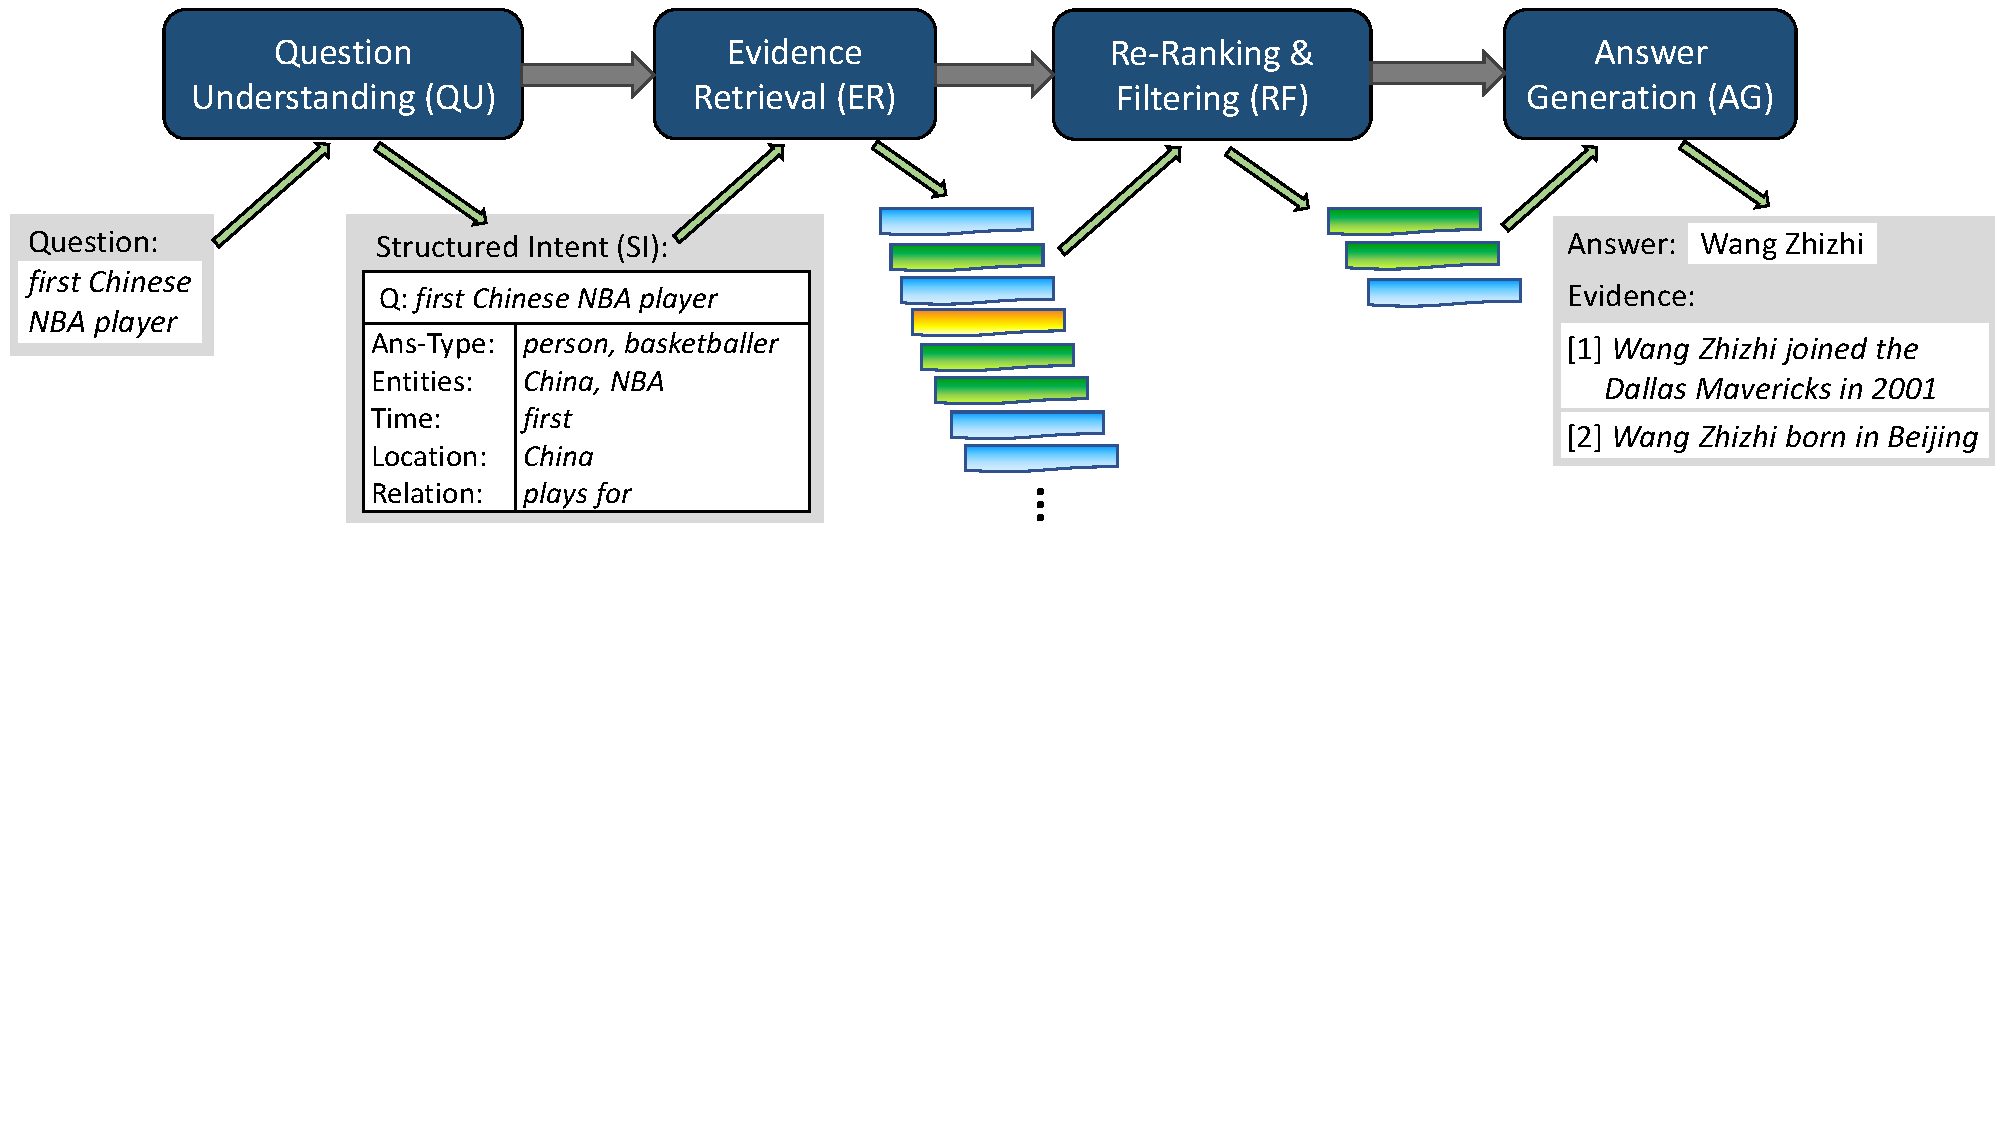
\includegraphics[width=\textwidth]{submissions/Gerhard2024/figures/compass-overview.pdf}
  \caption{Overview of the \method system.}
  \label{fig:compass-overview}
\end{figure}

% start with system overview
The \method system is a pipeline of four major stages, as illustrated in Figure \ref{fig:compass-overview}.
First, the input question is analyzed and decomposed, in order to compute a {\em structured intent (SI)} representation that will pass on to the subsequent steps, along with the original question. Second, the SI is utilized to retrieve pieces of evidence from different sources: text, KG and tables. 
Third, this pool of potentially useful evidence is filtered down, with iterative re-ranking, to arrive at a tractably small set of most promising evidence.
The final stage generates the answer from this evidence,
passing back the answer as well as evidence snippets for user-comprehensible explanation.

The second and fourth stage, Evidence Retrieval (ER) and Answer Generation (AG), are fairly standard. Such a two-phase architecture was called a retriever-reader architecture~\cite{Zhu-ODQA-survey:arxiv2021}. With a modern LLM replacing the earlier kinds of neural readers, this is the core of every RAG system~\cite{DBLP:journals/arXiv/abs-2312-10997}.

Stages 1 and 3 are unique elements of our architecture, judiciously introduced to improve both effectiveness (i.e., answer quality) and efficiency (i.e., computational cost).
Question Understanding (QU) provides the ER component with crisper and semantically refined input, and
the Re-Ranking \& Filtering (RF) stage is beneficial for
distilling the best evidence from the large pool of retrieved pieces.
The following subsections elaborate on the four stages of the pipeline, emphasizing the \method-specific steps QU and RF.



\subsection{Question Understanding (QU)}

% one par introducing the SI
To prepare the retrieval from different kinds of sources, including a KG, ad-hoc tables and text documents, it is useful to analyze and decompose the user question.
In this work, we aim to cast a question into a 
{\em structured intent (SI)} representation: essentially
a frame with faceted cues as slots, or equivalently, a concise set of key-value pairs. 
Figure \ref{fig:compass-overview} gives an idealized example for the question about the first Chinese NBA player. The facets or keys of potential interest here 
are:
\squishlist
\item {\em Ans-Type:} the expected answer type (or types when considering
different levels of semantic refinement), 
\item {\em Entities:} the salient entities in the question, and 
\item {\em Relation:} phrases that indicate which relation (between Q and A entities) the user is interested in. 
\squishend
\noindent In addition, as questions can have temporal or spatial aspects, the SI also foresees slots for:
\squishlist
\item {\em Time:} cues about answer-relevant time points or spans, including relative cues (e.g., ``before Covid'') and ordinal cues (e.g., ``first''), and
\item {\em Location:} cues about answer-relevant geo-locations.
\squishend

% discuss the spectrum of different SIs
\vspace{0.2cm}
\noindent The ideal SI for example question Q2 would look like:

\begin{quote}
{\em Ans-Type:} person, basketballer; {\em Entities:} China, NBA; {\em Time:} first;
{\em Location:} China; {\em Relation:} plays for.
\end{quote}

Note that the values for these slots can be crisp like entity names or dates, but they can also take the form of surface phrases. The SI purpose and value lie in the decomposition. In practice, many questions would only lead to a subset of faceted cues, leaving some slots empty. For the example in Figure \ref{fig:compass-overview}, an alternative SI could simply consist of

\begin{quote}
{\em Ans-Type:} person; {\em Entities:} China, NBA; {\em Time:} first.
\end{quote}

\noindent Even this simplified SI can be highly beneficial in guiding the subsequent evidence retrieval.

% sketch how an LM is trained to generate SIs 
To generate the SI from a user question, we employ a (small-scale) LM, specifically BART~\cite{DBLP:conf/acl/LewisLGGMLSZ20}, a Transformer-based auto-encoder with 140M parameters.\footnote{\url{https://huggingface.co/facebook/bart-base}}
BART is pre-trained for language representation; its power for our purpose comes from fine-tuning.
To this end, we generate (question, SI) pairs by using an instruction-trained LLM like GPT-4, with few-shot in-context learning (following our earlier work~\cite{Jia-FAITH:WWW2024}). 
Note that this is a one-time action; at inference-time we only use much smaller LMs.
The generated silver-standard pairs are then used to fine-tune BART.
In the experiments in this article, we leverage pre-existing collections of silver pairs, based on the training data of the CompMix benchmark~\cite{Christmann-CompMix:WWW2024}, 
comprising $3{,}400$ such pairs.


% outline value of SI for conversations
Although this paper focuses on single-shot questions, the \method architecture is also geared for conversational QA. In that setting, the SI can play an even bigger role, as (follow-up) questions are often formulated in a rather sloppy manner -- all but self-contained. For example, a conversation could start with a clear question {\em When did Wang Zhizhi join the NBA?}, followed a few dialog steps later, by a user utterance like {\em Which teams did he play for?} or simply {\em Which teams?}.
In such an informal conversation, the system needs to {\em contextualize} each user utterance based on the preceding turns in the dialog (e.g., inferring the relevant entities Wang Zhizhi and NBA from the conversational history).
For details on conversational QA, based on our architecture, see our earlier works~\cite{Christmann-CONVINSE:SIGIR2022,Christmann-Explaignn:SIGIR2023}.







%%%%%%%%%%%%%%%%%%%%%%%%%%%%%%%%%%%%%
\subsection{Evidence Retrieval (ER)}

The ER stage taps into a knowledge graph, a corpus of text documents, and a collection of web tables.
Specifically, for the experiments, we use the Wikidata KG,
all English Wikipedia articles, and all tables that are embedded in Wikipedia pages (incl. infoboxes, which can be seen as a special case of tables). 

% specifics: Clocq etc. - and the role of the SI
\vspace{0.2cm}
\noindent{\bf Retrieval from KG:}
To retrieve evidence from the KG, we utilize our earlier work
\clocq~\cite{Christmann-CLOCQ:WSDM2022}, which provides entity disambiguations and a relevant KG-subgraph for a given query.
Unlike most other works on QA-over-KG, \clocq fetches all KG-facts that are relevant for a given entity in a single step.
For example, when querying for
NBA players, it can traverse the KG neighborhood and pick up top teams, also considering so-called qualifier nodes in Wikidata which are often used for temporal scopes. 
As the disambiguation of entity names onto the KG can be tricky and noisy (e.g., China could be mapped to Chinese sports teams in all kinds of sports), \clocq considers several possible disambiguations~\cite{Christmann-CLOCQ:WSDM2022} (typically in the order of $10$ result entities).
The queries for \clocq are 
constructed by concatenating all slots of the question's SI.
For the example query about the first Chinese NBA player,
good result entities would be Dallas Mavericks, lists about NBA seasons, MVP awards etc., and their associated facts. These provide cues, but are likely insufficient to answer the question.


\vspace{0.2cm}
\noindent{\bf Retrieval from Text and Tables:}
The disambiguated entities returned by \clocq form anchors for tapping into text and tables.
\method first identifies 
relevant text documents and tables that refer to the anchor entities. With focus on Wikipedia, these are simply the articles for the respective entities. 
\method then constructs a keyword query that concatenates all available fields of the SI.
The query is evaluated against a linearized and verbalized representation (see below) of all sentences and all table rows in the selected documents.
This returns a set of sentences and 
and individual table rows, ranked by BM25 scores.


\vspace{0.2cm}
\noindent{\bf Evidence Verbalization:}
All results from the different data sources are uniformly treated by {\em linearizing} and {\em verbalizing} them
into token sequences. For KG results, the entity-centric triple sets are linearized via breadth-first traversal of the mini-graph starting from the entity node.
For tables, results are individual rows, which are contextualized by including labels from column headers and from the DOM-tree path of the article where the table comes from. For example, a table row about Wang Zhizhi playing for Dallas (Mavericks) in the 2000-2001 season, would be expressed as:

\vspace{0.05cm}
\hspace*{0.5cm} Wang Zhizhi / NBA Career / Season: 2000-2001, Team: Dallas, Games Played: 5 \dots
\vspace{0.05cm}

\noindent Finally, results from the text corpus are already in the form of token sequences, but we can additionally prefix these with the DOM-tree labels.
We can think of this entire pool of evidence as 
an on-the-fly corpus of potentially relevant pseudo-sentences, forming the input of the subsequent RF stage.


\vspace{0.2cm}
\noindent {\bf Result Ranking:}
Overall, the ER stage compiles a substantial set of evidence, possibly many thousands of entities, text snippets and table rows. Therefore, we practically restrict the pool to a subset of high-scoring pieces, like the top-$1000$.
For scoring, a simple BM25 model (a classical IR method) is applied. 
By default, we treat all evidence pieces uniformly with global scoring, no matter whether they come from KG, text or tables. 


\subsection{Re-Ranking and Filtering (RF)}

With a pool of top-$1000$ evidence pieces, we could invoke an LLM for answer generation. However, that would face a large fraction of noise (i.e., misleading evidence) and incur high costs of computation and energy consumption. 

For both of these reasons, we have devised light-weight techniques for iteratively reducing the top-$1000$ pieces to a small subset, say top-$30$ or top-$10$, that can be fed into an LLM at much lower cost (as LLM computations and pricing are at least linear in the number of input tokens). The difficulty is, of course, to do this without losing good evidence and reducing answer presence. Our techniques for this task are based on graph neural networks (GNNs)~\cite{Wu:IEEE2021} or cross-encoders (CEs)~\cite{Dejean:arxiv2024,Lin:MC2021}.

\myparagraph{GNN-based RF}
Given a large pool of evidence pieces from all sources, a bipartite graph is constructed:
\squishlist
\item {\em nodes} being evidence pieces or entities that occur in these pieces, and
\item {\em edges} connecting an evidence piece and an entity if the entity occurs in the evidence.
\squishend


The task for the GNN is to jointly score the evidence and the entity nodes in a multi-task learning setup. The latter are the {\em answer candidates}, and the evidence should give {\em faithful explanation} for an answer.
We build on our earlier work on explainable QA~\cite{Christmann-Explaignn:SIGIR2023}.

The node encodings are initialized with cross-encoder embeddings (see below) 
for node contents and the SI of the question. The inference iteratively adjusts the encodings based on message passing from neighboring nodes.
The GNN is trained via weak supervision from question-answer pairs:
evidence nodes are labeled as relevant if they are connected to
a gold answer.
More technical details are given in~\cite{Christmann-Explaignn:SIGIR2023}.

\method invokes the GNN in multiple rounds, iteratively reducing top-$k$ to top-$k^*$ nodes with $k^* \ll k$. In practice, we would typically consider two rounds: re-ranking top-$1000$ and pruning to top-100, and then reducing to top-30 or top-10, which are passed to the answer generation stage.
Note that this keeps the GNN at a tightly controlled size, so that its computational costs at inference-time are much smaller than those of an LLM.


\myparagraph{CE-based RF}
An alternative to the GNN inference is to employ a cross-encoder for scoring and re-ranking the evidence pieces.
These are transformers (typically with a small LM like BERT) that are fine-tuned for scoring the relatedness between a query and a document~\cite{Nogueira:arxiv2019}. In our case, the comparison is between the question SI and the evidence piece. In our experiments, we make use of two different cross-encoders, 
both trained on the MS-MARCO benchmark for passage retrieval~\cite{Bajaj:arxiv2018}, 
and fine-tuned on the respective benchmark (leveraging the same weak supervision data as for the GNNs),
the difference being in model size.\footnote{\url{https://huggingface.co/cross-encoder/ms-marco-MiniLM-L-4-v2} and\\ \url{https://huggingface.co/cross-encoder/ms-marco-MiniLM-L-6-v2}}
We use the smaller model to reduce top-$1000$ to top-100, and the larger model to go further down from top-100 to top-30.




%%%%%%%%%%%%%%%%%%%%%%%%%%%%%%%%%%%%%

\subsection{Answer Generation (AG)}

The last stage follows mainstream practice to invoke an LLM in a retrieval-augmented manner.
We call a `small-scale` LLM, specifically a fine-tuned LlaMA-3.1 model (8B-Instruct)\footnote{\url{https://huggingface.co/meta-llama/Llama-3.1-8B-Instruct}}, with a prompt \footnote{The specific prompt is \phrase{SI: \textless\texttt{concatenated SI}\textgreater \hspace{0.1cm} Evidence: \textless\texttt{evidence pieces}\textgreater}.}
consisting of:

\squishlist
\item the concatenated SI of the original question, and
\item the top-30 (or other top-$k^*$ with small $k^*$) evidence pieces.
\squishend

By the previous down-filtering of the original pool of evidence pieces, this last step has affordable cost in terms of computation time and energy consumption.

\vspace{0.2cm}
\noindent{\bf Fine-Tuning the LLM:}
We considered adding an instruction to the prompting, such as {\em ``answer this question solely based on the provided evidence snippets''}.
However, this turned out to be ineffective.
The reason why the model works well without such instructions is our task-specific fine-tuning.
We perform this by running the training data of benchmarks through the \method pipeline,
and training the AG stage with the top-30 evidence pieces as input.
Thus, the fine-tuning makes the model learn the role of evidence for RAG-based QA.

\vspace{0.2cm}
\noindent{\bf Explanations:}
The top-30 evidence pieces can be used to provide users with explanation of answers.
Optionally, these could be reduced further for comprehensibility.
Alternatively, we can fine-tune the LLM to provide both answers and concise explanations.
Since we can infer which evidences in the input mention the annotated ground-truth answers,
our method could be fine-tuned to provide such \textit{answering evidences} as well (cf.~\cite{Gao-citations:emnlp2023}).

\label{sec:exp}
\section{Experiments}


\label{setup}
\subsection{Experimental setup}


%%% BENCHMARKS
\myparagraphnospace{Benchmarks} We run experiments on three benchmarks with different characteristics of questions.

\squishlist
    \item \textbf{\compmix}.
    \compmix~\cite{Christmann-CompMix:WWW2024} is a benchmark which was specifically designed for evaluating QA systems operating over heterogeneous sources. The dataset has $9{,}410$ questions, out of which $2{,}764$ are used for testing.
    Answers are crisp entity names, dates, or other literals.
    
    \item \textbf{\crag}.
    We further evaluate on a subset of the \crag~\cite{Yang-CRAG} dataset, which was recently released as a testbed for RAG-based QA systems.
    We utilize the same pipeline and sources as outlined in Section~\ref{sec:method}, without using the web snippets or APIs provided with \crag. This way we focus on entity-centric questions that do not require access to live web data (e.g., news feeds), and disregard cases where the results would be up-to-date quantities.
    This restricts the test data to $436$ entity-centric questions, still enough for a proof of concept.
    
    \item \textbf{\timequestions}.
    To showcase the generalizability of our pipeline, we conduct experiments on~\timequestions~\cite{Jia-TimeQuestions},
    a benchmark for temporal QA. The dataset requires temporal understanding and reasoning, which are well-known limitations of
    LLMs~\cite{Dhingra-time-aware-LLM:TACL2022}. \timequestions has 16{,}181 questions (3{,}237 for testing).
\squishend

Typical examples for the questions in these three benchmarks are:

\begin{quote}
\compmix: \utterance{Which player won the most number of Man-of-the-Match titles in the FIFA world cup of 2006?}\\
 \indent \crag: \utterance{What was the worldwide box office sales for little hercules?}\\ 
  \indent \timequestions: \utterance{Which club did Cristiano Ronaldo play for before joining Real Madrid?}
\end{quote}

%%% BASELINES
\myparagraph{Baselines} As competitors or reference points to \method, we study the performance of the following methods:

\squishlist
    \item \textbf{Generative LLMs}.
    We compare \method against out-of-the-box LLMs: \textbf{\gptthree} (\texttt{text-davinci-003}), \textbf{\gptfour} (\texttt{gpt-4}) 
    and \textbf{\llama} (\texttt{meta-llama/Llama-3.1-8B-Instruct}).
    The same prompt is used for all LLMs, consistent with previous work~\cite{Christmann-CompMix:WWW2024, Zhang-Spaghetti:ACL2024}:
    \phrase{Please answer the following question by providing the crisp answer entity, date, year, or numeric number. Q: \textless\texttt{question}\textgreater}.
    

    \item \textbf{Heterogeneous QA methods}.
    \convinse~\cite{Christmann-CONVINSE:SIGIR2022}, \unikqa~\cite{Oguz-UniK-QA:NAACL2022}, \explaignn~\cite{Christmann-Explaignn:SIGIR2023}
    are QA methods designed to integrate heterogeneous sources: text, tables and KG. All of these  integrate the exact same sources as \method.

    
    \item \textbf{\textsc{State-of-the-art}}.
    For \compmix and \timequestions, we also compare against state-of-the-art methods from the literature: \spaghetti~\cite{Zhang-Spaghetti:ACL2024} and \textsc{Un-Faith}~\cite{Jia-FAITH:WWW2024}, which are among the best performing systems.
    
Results are taken from the literature whenever applicable.
On \crag, we use the models trained on \compmix for \method and heterogeneous QA baselines.
\squishend



%%% METRIC(S)
\myparagraph{Metrics}
We measure \textit{precision at 1} (\textbf{P@1}) as our main metric~\cite{RoyAnand:MC2021} on all benchmarks.
On \crag, we manually annotate answer correctness, as the ground-truth answer formats vary (e.g., entity name variants, lists, sentences).

We also compute the number of neural parameters aggregated over all sub-modules (\textbf{\#Parameters}).
Parameter counts for GPT-models are taken from~\cite{Minaee-LLM-survey}
(\gptfour might have less active parameters during inference).

For further analysis we measure \textit{answer presence} (\textbf{AP@k}),
i.e. whether the answer is present in the top-$k$ ranked evidence pieces,
and \textit{mean reciprocal rank} within the top-$k$ evidences (\textbf{MRR@k}).

%%% CONFIG
\myparagraph{Configuration}
Our implementation uses the \texttt{Llama3.1-8B-Instruct} model for the AG stage.
For the QU, ER and RF stages
we adopt code from the \explaignn project.\footnote{\url{https://explaignn.mpi-inf.mpg.de}}
For the ER stage, we use \clocq, setting its specific parameters to $k=10$ and $p=1{,}000$.

As default, we use the GNN technique for the RF stage.
For efficiency, we use light-weight models for initializing
the GNN encoders -- the same models used for the CE-based RF.\footnote{\url{https://huggingface.co/cross-encoder/ms-marco-MiniLM-L-4-v2} and\\\url{https://huggingface.co/cross-encoder/ms-marco-MiniLM-L-6-v2}}
The GNNs are trained for $5$ epochs with an epoch-wise evaluation strategy,
i.e. we choose the model with the best performance on the respective dev set.
We train the GNNs on graphs with a maximum of $100$ evidence and $400$ entity nodes (as scored by BM25).
During inference, the first GNN is applied on graphs with $1{,}000$ evidence and $4{,}000$ entity nodes, shrinking the pool of evidence pieces to the top-$100$.
The second GNN then runs on graphs with $100$ evidence and $400$ entity nodes.
The factor of 4 entities per evidence (on average) holds sufficient for the observed data,
and enables batched inference.
Other parameters are kept as is.

The AG model, based on \texttt{Llama3.1-8B-Instruct}, is 
fine-tuned
for $2$ epochs with a warm-up ratio of $0.01$ and a batch size of $8$, again with an epoch-wise evaluation strategy.
Other parameters are set to the default Hugging Face
training parameters.\footnote{\url{https://huggingface.co/docs/transformers/v4.46.2/en/main_classes/trainer\#transformers.TrainingArguments}}





\subsection{Main results}
%%% MAIN TABLE
\myparagraphnospace{\method is competitive on all benchmarks}
Main results of our experiments are shown in Table~\ref{tab:main-res}.
First of all, we note that \method achieves competitive performance across all three benchmarks.

On \compmix, baselines for heterogeneous QA and \llama perform similarly,
whereas GPT-based LLMs can answer more than $50$\% of the questions correctly.
\method exhibits substantially higher performance, on par with
the state-of-the-art method \textsc{Spaghetti}~\cite{Zhang-Spaghetti:ACL2024}
(which is based on \gptfour).

On the \crag dataset, P@1 drops for all methods except for \gptfour. 
The benchmark includes realistic questions,
which can be ambiguous/confusing (\phrase{who was the director for the report?}),
on ``exotic'' entities with answers in social media (\phrase{how many members does the teknoist have?}),
or require up-to-date information (\phrase{when did chris brown release a song or album the last time?}),
and other cases that are challenging for all methods.

Finally, \method establishes new state-of-the-art performance on the \timequestions benchmark.
Interestingly, all of the tested LLMs show greatly reduced performance on this benchmark,
which inherently requires temporal understanding and reasoning
-- a known weakness of stand-alone LLMs.


\begin{table} [h]
    \centering
    \newcolumntype{G}{>{\columncolor [gray] {0.90}}c}
    \begin{tabular}{l G G G c}
        \toprule
            \textbf{Method $\downarrow$ / Benchmark $\rightarrow$} & \textbf{\compmix}  & \textbf{\crag} & \textbf{\timequestions} & \textbf{\#Parameters} \\ 
        \midrule
            \textbf{\gptthree} 
            & $0.502$ &   $-$ & $0.224$ & $175{,}000$ M  \\
            % #params from https://arxiv.org/pdf/2402.06196

            \textbf{\gptfour}
            & $0.528$ &   $\mathbf{0.633}$ & $0.306$ & $1{,}760{,}000$ M \\
            % #params from https://arxiv.org/pdf/2402.06196

            \textbf{\llama~\cite{Touvron-LLaMA}} (8B-Instruct)
            & $0.431$ &   $0.385$ & $0.178$ & $8{,}030$ M  \\
            % #params from Huggingface (8,030,257,152)
        \midrule
            \textbf{\convinse~\cite{Christmann-CONVINSE:SIGIR2022}}
            & $0.407$  &   $0.298$ & $0.423$  & $362$ M \\
            % FiD: 222,903,936 + BART (SR-generation): 139,420,416 = 362,324,352 (python explaignn/question_understanding/structured_representation/get_num_params.py)

            \textbf{\unikqa~\cite{Oguz-UniK-QA:NAACL2022}}
            & $0.440$ &   $0.280$ & $0.424$ & $223$ M  \\
            % FiD: 222,903,936 (python explaignn/heterogeneous_answering/fid_module/FiD/get_num_params.py)
    
            \textbf{\explaignn~\cite{Christmann-Explaignn:SIGIR2023}} 
            & $0.442$ &   $0.303$ & $0.525$  & $328$ M \\
            % BART (SR-generation): 139,420,416 + 2GNNs: 94520832 + 93930240 = 327,871,488

        \midrule 
            \textbf{\textsc{State-of-the-art}}
            & $\mathbf{0.565}$ 
            & $-$
            & $0.571$  & $-$ \\

            & (\textsc{Spaghetti}~\cite{Zhang-Spaghetti:ACL2024})
            & 
            & (\textsc{Un-Faith}~\cite{Jia-FAITH:WWW2024}) &  \\

        \midrule
            \textbf{\method (ours)}
            & ${0.564}$ &   $0.362$ & $\mathbf{0.754}$  & $8{,}218$ M \\
            % BART (SR-generation): 139,420,416 + LLaMA: 8,030,257,152 + GNNs: 25,670,016 + 22,268,928 =  8,217,616,510
        \bottomrule
    \end{tabular} 
    \vspace*{-0.2cm}
    \caption{End-to-end P@1 of \method and baselines on three benchmarks. Results for \gptthree and \gptfour are taken from the literature~\cite{Christmann-CompMix:WWW2024, Jia-FAITH:WWW2024}. \gptthree is not accessible anymore, hence no results on \crag.
    }
    \label{tab:main-res}
\end{table}





%%% ANSWER SOURCES
\myparagraph{Integration of heterogeneous sources is vital}
\method integrates evidence from text, KG and tables into a unified framework.
We aim to better understand how this affects the answering performance of the method.
Table~\ref{tab:sources} shows end-to-end answering performance of \method
with different combinations of the input sources.
The results clearly indicate that all types of sources contribute, with option Text+KG+Tables performing best,
with a large margin over tapping only single source types.

\begin{table} [t] 
    \centering
    \newcolumntype{G}{>{\columncolor [gray] {0.90}}c}
    \newcolumntype{H}{>{\setbox0=\hbox\bgroup}c<{\egroup}@{}}
    	\begin{tabular}{l G G G H H H c c c} 
        \toprule
            \textbf{Benchmark $\rightarrow$}
                & \multicolumn{3}{G}{\textbf{\compmix}} 
                & \multicolumn{3}{H}{\textbf{\crag}}
                & \multicolumn{3}{c}{\textbf{\timequestions}} \\ 
        \midrule
            \textbf{Input sources $\downarrow$ / Metric $\rightarrow$}
                & \textbf{P@1} & \textbf{AP@100}  & \textbf{AP@30}
                & \textbf{P@1} & \textbf{AP@100}  & \textbf{AP@30}
                & \textbf{P@1} & \textbf{AP@100}  & \textbf{AP@30} \\
            \midrule
                \textbf{Text}           &  $0.455$  &  $0.563$  &  $0.531$ &  $?$  &  $?$  &  $?$ &  $0.539$  &  $0.515$  &  $0.487$   \\
                \textbf{KG}             &  $0.481$  &  $0.677$  &  $0.637$ &  $?$  &  $?$  &  $?$ &  $0.724$  &  $0.701$  &  $0.674$   \\
                \textbf{Tables}         &  $0.432$  &  $0.501$  &  $0.482$ &  $?$  &  $?$  &  $?$ &  $0.536$  &  $0.347$  &  $0.328$   \\
            \midrule
                \textbf{Text+KG}        &  $0.537$  &  $0.749$  &  $0.706$ &  $?$  &  $?$  &  $?$ &  $0.745$  &  $\mathbf{0.776}$  &  $0.748$   \\
                \textbf{Text+Tables}    &  $0.503$  &  $0.632$  &  $0.594$ &  $?$  &  $?$  &  $?$ &  $0.567$  &  $0.578$  &  $0.549$   \\
                \textbf{KG+Tables}      &  $0.524$  &  $0.728$  &  $0.692$ &  $?$  &  $?$  &  $?$ &  $ 0.743$  &  $0.731$  &  $0.703$   \\
            \midrule
                \textbf{Text+KG+Tables}    &  $\mathbf{0.564}$  &  $\mathbf{0.759}$  &  $\mathbf{0.724}$ &  $?$ &  $?$  &  $?$ & $\mathbf{0.754}$    & $\mathbf{0.776}$  &  $\mathbf{0.749}$   \\
            \bottomrule
    \end{tabular}
    \vspace*{-0.2cm}
    \caption{Answer presence and answering precision of \method with different combinations of input sources (on the respective test sets).}
    \label{tab:sources}
\end{table}




\subsection{Analysis}

%%% TOP-K vs. 3xTOP-(K/3)
\myparagraph{Unified retrieval enhances performance}
In the RF stage, we re-rank and filter evidence from different source types,
and feed the unified top-\textit{k}* into the AG stage.
We conduct a comparison in which we consider
the top-$10$ evidence pieces from each source type individually. This gives equal influence to KG, text and tables, whereas our default is based on global ranking.
Table~\ref{tab:unified-retrieval} shows the results for this analysis, showing our default choice performs better.
The reason is that different questions require different amounts of evidence from each of the source types.

\begin{table} [t] 
    \centering
    \newcolumntype{G}{>{\columncolor [gray] {0.90}}c}
    \newcolumntype{H}{>{\setbox0=\hbox\bgroup}c<{\egroup}@{}}
    	\begin{tabular}{l G G H H} 
        \toprule
            \textbf{Input evidences $\downarrow$ / Metric $\rightarrow$} & \textbf{P@1} & \textbf{AP@30}  & \textbf{\crag} & \textbf{\timequestions} \\ 
            \midrule
                \textbf{Top-30 Text+KG+Tables (ours)}             &  $\mathbf{0.574}$  &  $\mathbf{0.710}$  &  $-$  &  $-$   \\
                \textbf{Top-10 Text + Top-10 KG + Top-10 Tables}        &  $0.560$    &  $0.709$  &  $-$  &  $-$   \\
            \bottomrule
    \end{tabular}
    \vspace*{-0.2cm}
    \caption{Answer presence and precision
    of \method for different choices of top-30 
    (on \compmix dev set).}
    \label{tab:unified-retrieval}
\end{table}


%%% NUMBER OF EVIDENCES
\myparagraph{\method works well with small amounts of evidence}
We investigate the 
influence of 
the number of evidence pieces
fed into the AG stage, varying it from $5$ to $100$.
Results are shown in Figure~\ref{fig:res-num-evidences}.
As the curve shows, there is a sharp increase in precision as we add evidence up to 30 or 40 pieces, which is around our default of top-30. This indicates that a certain amount of evidence is needed, to overcome the inherent noise and arrive at sufficient answer presence. 
As we increase the amount of evidence further, we observe a saturation effect, and eventually a degration of performance. Too much evidence not only has diminishing returns, but can actually be confusing for the AG stage. This reconfirms our heuristic choice of top-30: enough for good answering while keeping computational costs reasonably low.


\begin{figure}[t]
    \centering
    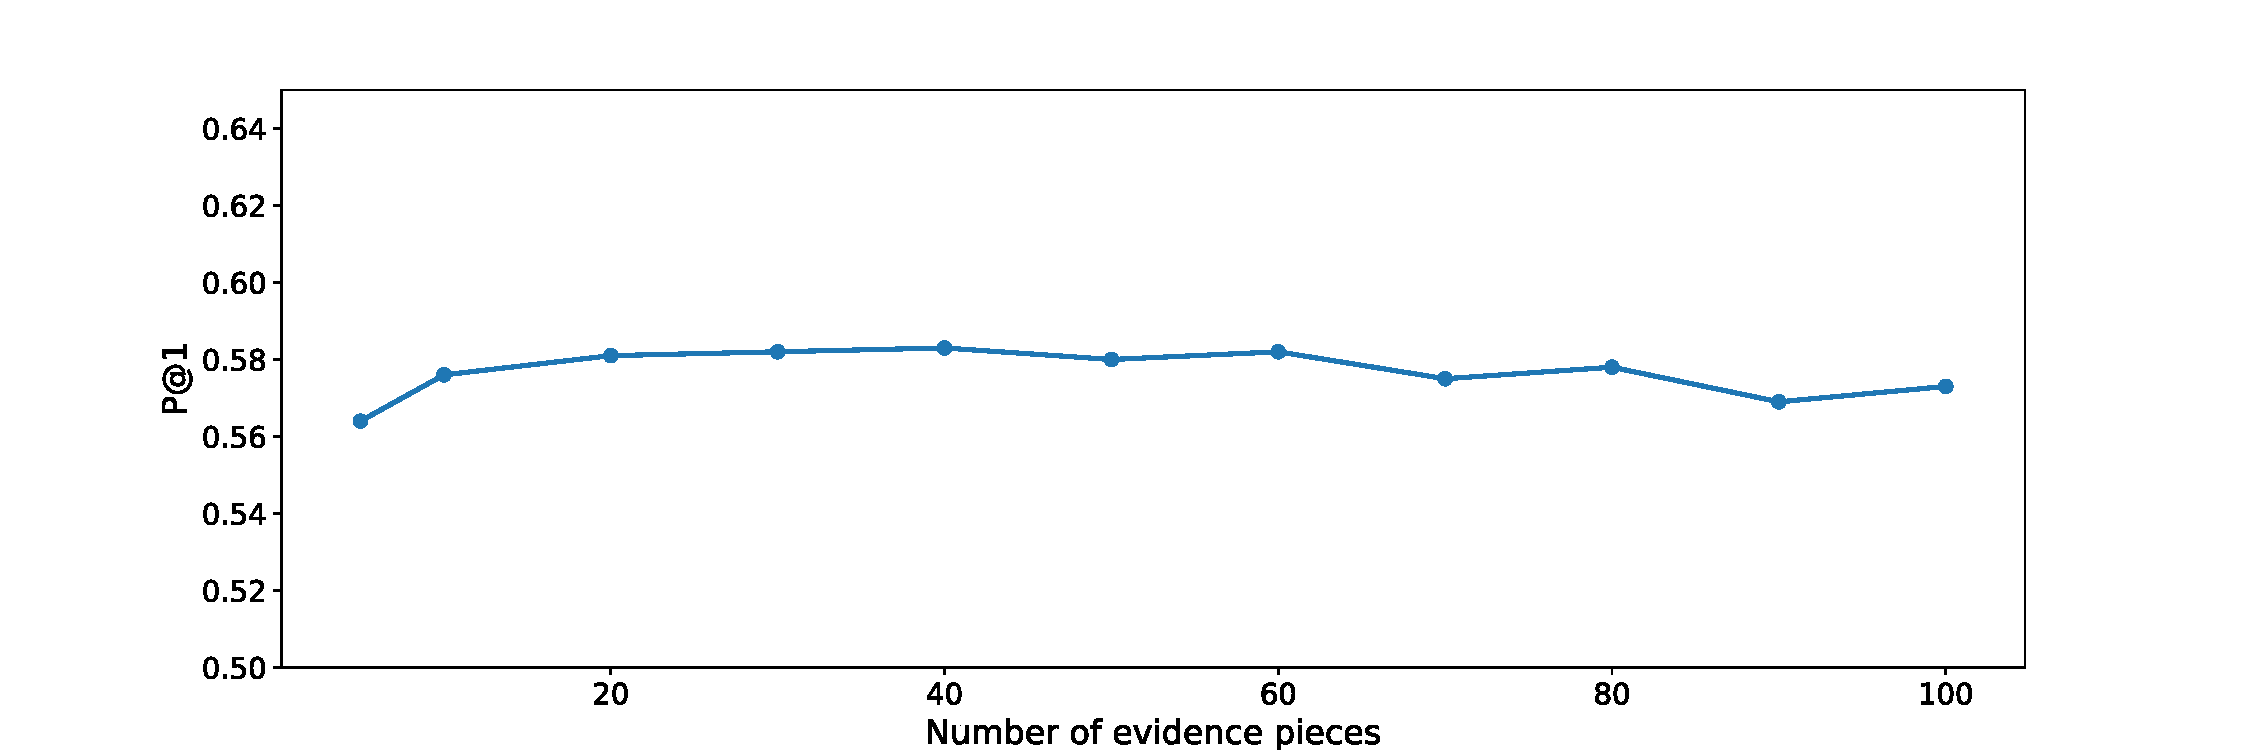
\includegraphics[width=0.8\textwidth]{submissions/Gerhard2024/figures/p_at_1-line_with_evidences.pdf}
    \vspace*{-0.2cm}
    \caption{Performance of \method on the \compmix dev set with different numbers of evidence.}
    \label{fig:res-num-evidences}
    \vspace*{-0.2cm}
\end{figure}



%%% ABLATION
\myparagraph{Ablation study on re-ranking} For more insight on the possible configurations of the RF stage, we conducted an ablation study with different options, including solely relying on the initial BM25 scoring without explicit re-ranking. The results are shown in Table \ref{tab:ablation2}. We observe that the iterative reduction in two steps is slightly better than the single-step variants (going down from top-1000 to top-30 in one RF step). Between the two options of using a GNN or a CE, the differences are negligible. A notable effect is that our RF techniques retain the answer presence at a very high level, only a bit lower than for the initial top-1000. 
The last two rows of Table \ref{tab:ablation2} demonstrate that RF is crucial: without explicit re-ranking, the technique of just picking smaller top-$k$ from the original BM25 model leads to substantial degradation in both answer presence and precision. 


\begin{table} [t] \small
    \centering
    \newcolumntype{G}{>{\columncolor [gray] {0.90}}c}
    \newcolumntype{H}{>{\setbox0=\hbox\bgroup}c<{\egroup}@{}}
    	\begin{tabular}{l G H G G G} 
        \toprule
            & \multicolumn{5}{G}{\textbf{\compmix} (dev set)} \\
        \midrule
            \textbf{RF Method $\downarrow$ / Metric $\rightarrow$} & \textbf{P@1} & \textbf{AP@1000} & \textbf{AP@100}  & \textbf{AP@30} & \textbf{MRR@100} \\ 
        \midrule
            \textbf{GNN: 1000 $\rightarrow$ 100 $\rightarrow$ 30}             &  $\mathbf{0.574}$  & $0.760$ &  $0.738$  &  $0.710$  &  $\mathbf{0.572}$  \\
            \textbf{CE: 1000 $\rightarrow$ 100 $\rightarrow$ 30}          &  $0.573$  & $0.760$  &   $\mathbf{0.740}$ &  $\mathbf{0.721}$   &  $0.553$   \\
        \midrule
            \textbf{GNN: 1000 $\rightarrow$ 30} &  $0.567$  & $?$  &   $n/a$ &  $0.710$   &  $0.567$   \\
         \textbf{CE: 1000 $\rightarrow$ 30} &  $0.570$  & $0.760$  &   $n/a$ &  $0.715$   &  $0.558$   \\
            \midrule
           \textbf{BM25: 100 (w/o GNN or CE)} &  $0.490$ & $0.760$  &  $0.652$  &  $n/a$  &  $0.259$ \\       
            \textbf{BM25: 30 (w/o GNN or CE)} &  $0.468$  & $0.760$  &  $n/a$ &  $0.534$   &  $0.259$   \\
            \bottomrule
    \end{tabular}
    \vspace*{-0.2cm}
    \caption{Ablation study for different RF strategies of \method on the \compmix dev set. The answer presence in the RF input with top-$1000$ evidence pieces is $0.760$.}
    \label{tab:ablation2}
\end{table}



\myparagraph{Quality of SI}
To assess the quality and robustness of the Structured Intents, we
inspected a sample of questions and their SIs.
Table~\ref{tab:question-SI-examples} gives three anecdotic examples.
We show SIs generated by \method, which makes use of the pre-existing collection from the \compmix benchmark for training.
This training data was obtained via different heuristics, 
which can be a limiting factor when user intents become more complex.

Therefore, we also looked at SIs derived via in-context learning (ICL) using \gptfour with $5$ handcrafted examples.
As shown in our earlier work on temporal QA~\cite{Jia-FAITH:WWW2024},
such data can be used for training smaller models (e.g., BART),
which can greatly boost the completeness and overall quality of the generated SIs.

From the sampled set, we observed that the ICL-based SIs are more
complete with all slots filled, whereas the BART-based SIs focused more
on the main slots Answer-type, Entities and Relation.
However, both approaches achieve very high quality in filling the slots,
capturing the user's information need very well.

Interestingly, when questions get complicated, with nested phrases, 
the ICL-based variant succeeds in decomposing the questions, based on only $5$ ICL examples.
For example, for the question {\em ``which German state had the most Corona-related death cases in the first year after the outbreak?''}
the Time slot becomes {\em ``first year after Corona outbreak''},
which can be resolved to identify the temporal scope.
In general, we believe that such question decomposition, beyond simple temporal constraints,
would be an interesting theme for future work.

\begin{table} [t] 
    \centering
    \small
    \newcolumntype{G}{>{\columncolor [gray] {0.90}}c}
    \newcolumntype{H}{>{\setbox0=\hbox\bgroup}c<{\egroup}@{}}
    \resizebox*{\textwidth}{!}{
        \begin{tabular}{p{6cm}|p{6cm}|p{6cm}} 
        \toprule
            \textbf{Question} & \textbf{Current SI by \method} & \textbf{SI via ICL} \\
        \midrule
        \textit{what was disneys first color movie?}
            & Ans-Type: \textit{animated feature film} & Ans-Type: \textit{film, animated film} \\
            & Entities: \textit{disneys} & Entities: \textit{Disney} \\
            & Relation: \textit{was first color movie} & Relation: \textit{first color movie} \\
            &  & Time: \textit{first} \\
        \midrule
        \textit{at the oscars, who won best actor in 2018?}
            & Ans-Type: \textit{human} & Ans-Type: \textit{person, actor} \\
            & Entities: \textit{at the oscars} & Entities: \textit{Oscars, 2018} \\
            & Relation: \textit{who won best actor in 2018} & Relation: \textit{won best actor} \\
            &  & Time: \textit{2018} \\
        \midrule
        \textit{which German state had the most Corona-} & Ans-Type: \textit{state} & Ans-Type: \textit{location, state} \\
        \textit{related death cases in the first year after} & Entities: \textit{Germany, Corona} & Entities: \textit{Germany, Corona-related deaths} \\
        \textit{the outbreak?} & Relation: \textit{which state had the most related} & Relation: \textit{highest count of death cases} \\
        & \textit{death cases in the first year after the out-}  & Location: \textit{Germany} \\
            & \textit{break}  & Time: \textit{first year after Corona outbreak} \\
        \bottomrule
    \end{tabular}
    }
    \vspace*{-0.2cm}
    \caption{Examples for pairs of question and generated SI.}
    \label{tab:question-SI-examples}
\end{table}




%%% REFRAIN FROM ANSWER
\myparagraph{Refraining from answering}
%%% Searched for: "generated_answer I" (with I being the full word, not partial) in the generated answers of LLaMA
%%% yields 245 results out of 2764 questions on CompMix
%%% yields 1270 results out of 3237 questions on TimeQuestions
We can train our model to refrain from answering in scenarios
where the provided evidence does not contain an answer to the question.
Specifically, during training, when the answer is not present in the evidence,
we change the target answer to {\em unknown}. This variant is referred to as \method {\em (faithful)}.

We measure the ratio of questions for which {\em unknown} is provided as answer,
and the P@1 restricted to questions that are answered.
The accuracy of refraining from answering is measured as well,
based on whether the answer is present in the evidence or not.
We conduct this experiment on \compmix and \timequestions,
for which we can compute answer presence exactly.
We also compute results for \llama, which is already instructed 
with the option to answer ``don't know''.
Table~\ref{tab:refrain-from-answer} shows the results.
For \compmix, we observe that \method has high accuracy on refraining when appropriate,
whereas \llama tends to be overconfident with a very small rate of {\em unknowns}, leading to incorrect answers.

\begin{table} [t] \small
    \centering
    \newcolumntype{G}{>{\columncolor [gray] {0.90}}c}
    \newcolumntype{H}{>{\setbox0=\hbox\bgroup}c<{\egroup}@{}}
    	\begin{tabular}{l G G G G c c c c} 
        \toprule
            & \multicolumn{4}{G}{\textbf{\compmix}} & \multicolumn{4}{c}{\textbf{\timequestions}} \\
            \midrule
            \textbf{Metric $\rightarrow$} & \textbf{P@1}  & \textbf{P@1} & \textbf{Refrain} & \textbf{Refrain} & \textbf{P@1}  & \textbf{P@1} & \textbf{Refrain} & \textbf{Refrain} \\ 
            \textbf{Method $\downarrow$} &                 & \textbf{(answered)} & \textbf{rate} & \textbf{accuracy} &                 & \textbf{(answered)} & \textbf{rate} & \textbf{accuracy} \\ 
            \midrule
                \textbf{\llama}             &  $0.431$  &  $0.471$  &  $0.089$  &  $n/a$  &  $0.177$  &  $0.276$  &  $0.392$  &  $n/a$  \\
                \textbf{\method (faithful)}           &  $0.497$  &  $0.713$  &  $0.303$  &  $0.838$ &  $0.597$  &  $0.804$  &  $0.257$  &  $0.864$  \\
            \bottomrule
    \end{tabular}
    \vspace*{-0.2cm}
    \caption{
        Performance of \method with option to refrain from answering (``don't know'').
    }
    \label{tab:refrain-from-answer}
\end{table}

\label{sec:disc}
\section{Insights, Limitations, and Challenges}


\noindent{\bf Benchmark Performance.} Our method, RAG-based \method with an 8B LLaMA model, outperforms much larger LLMs like \gptfour on two of the three benchmarks, with a very large margin for temporal questions. Obviously, pre-trained LLMs have only limited sense of properly positioning ``remembered’’ facts on the timeline even with training data that exceeds ours by several orders of magnitude. This confirms our intuition that LLMs alone are not good at ``recalling’’  higher-arity relations that require combining distant pieces of evidence. This is a sweet spot for RAG. Only for 
the \crag benchmark, \method is substantially inferior to a full-blown LLM. This is likely due to the nature of the questions: not necessarily the complexity of the information needs, but the need for more web sources (beyond what our experiments tap into).

\vspace{0.2cm}
\noindent{\bf Cost/Performance Ratio.} The most important take-away from our experiments is that \method achieves its competitive performance at a much lower cost than the full LLMs. Assuming that the consumed GFlops are proportional to the number of model parameters, \method achieves a cost reduction by a factor of 200x for \gptthree and 2000x for \gptfour. This does not only mean less computation, but also a massively lower electricity bill and climate impact.  

\vspace{0.2cm}
\noindent{\bf Role of Question Understanding.} We did not systematically investigate the influence of the Structured Intent in the \method pipeline. However, the comparison to the big GPT models reflects the role of the SI, as we prompt the GPT models in their natural mode with the original questions. The linearized sequence of available SI slots does not always have major advantages, but there are enough cases where specific facets provide crucial cues. This holds especially for the Entities slot, as this drives the gathering of evidence in the ER stage (cf.~\cite{Christmann-CONVINSE:SIGIR2022}, and for the Time slot, as these cues are often decisive for temporal questions (cf.~\cite{Jia-FAITH:WWW2024}).

\vspace{0.2cm}
\noindent{\bf Role of Re-Ranking.} As our ablation studies show, merely using top-$k$ evidence from an initial BM25-style ranking does not provide good performance. Also, there seems to be sweet spot in the choice of $k$: we need enough evidence for connecting the dots if the question requires multiple pieces of information, or for corroborating candidates if the question finds many useful but noisy pieces. In the experiments, $k=30$ turns out to be good choice; much lower $k$ results in insufficient evidence, and much larger $k$ leads to saturation and ultimately degrading performance. Our argument for iteratively shrinking the candidate set in multiple rounds of re-ranking is substantiated in our experiments, but the gain of doing this, compared to GNN- or CE-based re-ranking from 1000 to 30, is not big. More research is called to better understand the role of ranking in RAG. 

\vspace{0.2cm}
\noindent{\bf Limitations of Evidence Retrieval.}
For ER, we adopted more or less standard techniques. The results showed very good answer presence, in the order of 75\% in the top-100 or even top-30. An important case where this is insufficient are questions that require aggregating information over a large number of evidence pieces. An example is asking for the life-time total of 3-point scores of the basketball player Dirk Nowitzki.
This requires collecting a set of per-season tables with NBA player statistics, but also other web sources with numbers for his career before he joined the NBA (including his youth teams).
Of course, there are sometimes shortcuts like a Wikipedia article or biography mentioning the total number, but this cannot be universally assumed. The bottom line is that ER should be reconsidered as well, striving to improve the recall dimension.

\vspace{0.2cm}
\noindent{\bf Limitations of Answer Generation.}
For AG, we simply rely on a LLM,
using it as an extractor (``reader'') from the given evidence. Despite the wide belief that LLMs can perform deep
reasoning over many pieces of evidence, our experience is that the extraction works only well – robustly and faithfully – for relatively simple questions with a few multi-hop joins or simple aggregation over a few pieces. However, complicated questions such as asking for the top-100 NBA players with the largest number of life-time 3-point scores (again including their pre-NBA careers) are currently out of scope and will likely remain so for quite some time. This offers many opportunities for pushing the envelope further.

\vspace{0.2cm}
\noindent{\bf Trust in Data Sources.}
In our experiments, we considered all heterogeneous sources as trustworthy and unbiased. With focus on Wikidata and Wikipedia, this assumption has been well justified. In the wild, however, input data for RAG-based systems likely exhibit a wide spectrum of quality issues, in terms of stale information, biased positions, or simply false statements. Identifying trustworthy and up-to-date evidence and dealing with conflicting data, has been explored in other contexts (e.g., for KG curation~\cite{Dong-Trust:PVLDB2015}), but remains a major challenge for RAG-based QA.


\vspace{0.2cm}
\noindent{\bf Open Challenges and Future Work.} The best-performing methods in our experiment, mostly \method, reach P@1 values of 56\% for \compmix and 75\% for \timequestions. 
For the latter, the answer presence in the top-100 is only slightly higher; so the AG stage hardly misses anything.
However, for \compmix, the answer presence is 75\% -- much higher than what our system can actually answer. Obviously, closing this gap is a major direction to pursue, with focus on the RF and AG stages. However, missing one fourth of the answers completely in the top-100 pool, is a big problem as well. This requires improving recall at the ER stage, possibly with better guidance by the QU, which in turn needs more sources beyond the scope of our experiments (currently limited to Wikidata and Wikipedia). 

In general, we need to think beyond this kind of ``benchmark mindset’’. Even if we reached 80\% or 90\% precision and recall, we would still have a substantial fraction of questions that are answered incorrectly
or not at all. 
The remaining errors may not be a problem for chatbots, but they would be a showstopper for the deployment of mission-critical applications in business or science. We believe that this big gap is a shortcoming of {\em all methods}, not an issue that comes from the data alone. For trivia-style QA, as looked at in this paper, a smart human in ``open book’’ mode and no time limitation should be able to properly answer practically all questions, just by reading pieces of web contents and putting things together. Neither LLMs nor state-of-the-art RAG are the final solution; substantial research and creative ideas are needed to further advance QA.


\clearpage
\newpage

\newcommand{\bibauthors}[1]{{#1}}
\newcommand{\bibtitle}[1]{\emph{#1}}
\newcommand{\bibconf}[1]{{#1}}

\begin{thebibliography}{10}

\bibitem{Bajaj:arxiv2018}
\bibauthors{Payal Bajaj, Daniel Campos, Nick Craswell, Li Deng, Jianfeng Gao, Xiaodong Liu, Rangan Majumder, Andrew McNamara, Bhaskar Mitra, Tri Nguyen, Mir Rosenberg, Xia Song, Alina Stoica, Saurabh Tiwary, Tong Wang.}
\bibtitle{MS MARCO: A Human Generated MAchine Reading COmprehension Dataset.}
In \bibconf{arXiv 2018}.

\bibitem{DBLP:conf/acl/ChenFWB17}
\bibauthors{Danqi Chen, Adam Fisch, Jason Weston and Antoine Bordes.}
\bibtitle{Reading Wikipedia to Answer Open-Domain Questions.}
In \bibconf{ACL 2017}.

\bibitem{Christmann-CONVINSE:SIGIR2022}
\bibauthors{Philipp Christmann, Rishiraj Saha Roy, Gerhard Weikum.}
\bibtitle{Conversational Question Answering on Heterogeneous Sources.}
In \bibconf{SIGIR 2022}.

\bibitem{Christmann-CLOCQ:WSDM2022}
\bibauthors{Philipp Christmann, Rishiraj Saha Roy, Gerhard Weikum.}
\bibtitle{Beyond NED: Fast and Effective Search Space Reduction for Complex Question Answering over Knowledge Bases.}
In \bibconf{WSDM 2022}.

\bibitem{Christmann-Explaignn:SIGIR2023}
\bibauthors{Philipp Christmann, Rishiraj Saha Roy, Gerhard Weikum.}
\bibtitle{Explainable Conversational Question Answering over Heterogeneous Sources via Iterative Graph Neural Networks.}
In \bibconf{SIGIR 2023}.

\bibitem{Christmann-CompMix:WWW2024}
\bibauthors{Philipp Christmann, Rishiraj Saha Roy, Gerhard Weikum.}
\bibtitle{CompMix: A Benchmark for Heterogeneous Question Answering.}
In \bibconf{WWW 2024}.

\bibitem{Dejean:arxiv2024}
\bibauthors{Herve Dejean, Stephane Clinchant, Thibault Formal.}
\bibtitle{A Thorough Comparison of Cross-Encoders and LLMs for Reranking SPLADE.}
In \bibconf{arXiv 2024}.

\bibitem{Dhingra-time-aware-LLM:TACL2022}
\bibauthors{Bhuwan Dhingra, Jeremy R Cole, Julian Martin Eisenschlos, Daniel Gillick, Jacob Eisenstein, and William W Cohen.}
\bibtitle{Time-Aware Language Models as Temporal Knowledge Bases.}
In \bibconf{TACL 2022}.

\bibitem{Dong-Trust:PVLDB2015}
\bibauthors{Xin Luna Dong, Evgeniy Gabrilovich, Kevin Murphy, Van Dang, Wilko Horn, Camillo Lugaresi, Shaohua Sun, Wei Zhang.}
\bibtitle{Knowledge-Based Trust: Estimating the Trustworthiness of Web Sources.}
In \bibconf{PVLDB 2015}.

\bibitem{DBLP:journals/arXiv/abs-2312-10997}
\bibauthors{Yunfan Gao, Yun Xiong, Xinyu Gao, Kangxiang Jia, Jinliu Pan, Yuxi Bi, Yi Dai, Jiawei Sun, Qianyu Guo, Meng Wang, Haofen Wang.}
\bibtitle{Retrieval-Augmented Generation for Large Language Models: A Survey.}
In \bibconf{arXiv 2023}.

\bibitem{Gao-citations:emnlp2023}
\bibauthors{Tianyu Gao, Howard Yen, Jiatong Yu, Danqi Chen.}
\bibtitle{Enabling Large Language Models to Generate Text with Citations.}
In \bibconf{EMNLP 2023}.

\bibitem{Guu-REALM:ICML2020}
\bibauthors{Kelvin Guu, Kenton Lee, Zora Tung, Panupong Pasupat, Ming-Wei Chang.}
\bibtitle{Retrieval Augmented Language Model Pre-Training.}
In \bibconf{ICML 2020}.

\bibitem{DBLP:conf/eacl/IzacardG21}
\bibauthors{Gautier Izacard, Edouard Grave.}
\bibtitle{Leveraging Passage Retrieval with Generative Models for Open Domain Question Answering.}
In \bibconf{EACL 2021}.

\bibitem{Jia-TimeQuestions}
\bibauthors{Zhen Jia, Soumajit Pramanik, Rishiraj Saha Roy, and Gerhard Weikum.}
\bibtitle{Complex Temporal Question Answering on Knowledge Graphs.}
In \bibconf{CIKM 2021}.

\bibitem{Jia-FAITH:WWW2024}
\bibauthors{Zhen Jia, Philipp Christmann, Gerhard Weikum.}
\bibtitle{Faithful Temporal Question Answering over Heterogeneous Sources.}
In \bibconf{WWW 2024}.

\bibitem{DBLP:journals/arXiv/abs-2305-06984}
\bibauthors{Ehsan Kamalloo, Nouha Dziri, Charles L. A. Clarke, Davood Rafiei.}
\bibtitle{Evaluating Open-Domain Question Answering in the Era of Large Language Models.}
In \bibconf{arXiv 2023}.

\bibitem{Kandpal:ICML2023}
\bibauthors{Nikhil Kandpal, Haikang Deng, Adam Roberts, Eric Wallace, Colin Raffel.}
\bibtitle{Large Language Models Struggle to Learn Long-Tail Knowledge.}
In \bibconf{ICML 2023}.

\bibitem{DBLP:conf/emnlp/KarpukhinOMLWEC20}
\bibauthors{Vladimir Karpukhin, Barlas Oguz, Sewon Min, Patrick S. H. Lewis, Ledell Wu, Sergey Edunov, Danqi Chen, Wen-tau Yih.}
\bibtitle{Dense Passage Retrieval for Open-Domain Question Answering.}
In \bibconf{EMNLP 2020}.

\bibitem{Lee-MATTER:ACL2024}
\bibauthors{Dongkyu Lee, Chandana Satya Prakash, Jack FitzGerald, Jens Lehmann.}
\bibtitle{MATTER: Memory-Augmented Transformer Using Heterogeneous Knowledge Sources.}
In \bibconf{ACL 2024}.

\bibitem{DBLP:conf/acl/LewisLGGMLSZ20}
\bibauthors{Mike Lewis, Yinhan Liu, Naman Goyal, Marjan Ghazvininejad, Abdelrahman Mohamed, Omer Levy, Veselin Stoyanov, Luke Zettlemoyer.}
\bibtitle{BART: Denoising Sequence-to-Sequence Pre-training for Natural Language Generation, Translation, and Comprehension.}
In \bibconf{ACL 2020}.

\bibitem{DBLP:conf/nips/LewisPPPKGKLYR020}
\bibauthors{Patrick S. H. Lewis, Ethan Perez, Aleksandra Piktus, Fabio Petroni, Vladimir Karpukhin, Naman Goyal, Heinrich Küttler, Mike Lewis, Wen-tau Yih, Tim Rocktäschel, Sebastian Riedel, Douwe Kiela.}
\bibtitle{Retrieval-Augmented Generation for Knowledge-Intensive NLP Tasks.}
In \bibconf{NeurIPS 2020}.

\bibitem{Lin:MC2021}
\bibauthors{Jimmy Lin, Rodrigo Frassetto Nogueira, Andrew Yates.}
\bibtitle{Pretrained Transformers for Text Ranking: BERT and Beyond.}
In \bibconf{Morgan \& Claypool Publishers 2021}.

\bibitem{Liu-SUQL:NAACL2024}
\bibauthors{Shicheng Liu, Jialiang Xu, Wesley Tjangnaka, Sina J. Semnani, Chen Jie Yu, Monica Lam.}
\bibtitle{SUQL: Conversational Search over Structured and Unstructured Data with Large Language Models.}
In \bibconf{NAACL-HLT 2024}.

\bibitem{Mavi:FnT2024}
\bibauthors{Vaibhav Mavi, Anubhav Jangra, Adam Jatowt.}
\bibtitle{Multi-hop Question Answering.}
In \bibconf{Foundations and Trends in Information Retrieval 2024}.

\bibitem{Minaee-LLM-survey}
\bibauthors{Shervin Minaee, Tomas Mikolov, Narjes Nikzad, Meysam Chenaghlu, Richard}
\bibtitle{Socher, Xavier Amatriain, and Jianfeng Gao.}
Large Language Models: A Survey.
In \bibconf{arXiv 2024}.

\bibitem{Nogueira:arxiv2019}
\bibauthors{Rodrigo Frassetto Nogueira, Kyunghyun Cho.}
\bibtitle{Passage Re-ranking with BERT.}
In \bibconf{arXiv 2019}.

\bibitem{Oguz-UniK-QA:NAACL2022}
\bibauthors{Barlas Oguz, Xilun Chen, Vladimir Karpukhin, Stan Peshterliev, Dmytro Okhonko, Michael Sejr Schlichtkrull, Sonal Gupta, Yashar Mehdad, Scott Yih.}
\bibtitle{UniK-QA: Unified Representations of Structured and Unstructured Knowledge for Open-Domain Question Answering.}
In \bibconf{NAACL-HLT 2022}.

\bibitem{RogersGA:CS2023}
\bibauthors{Anna Rogers, Matt Gardner, Isabelle Augenstein.}
\bibtitle{QA Dataset Explosion: A Taxonomy of NLP Resources for Question Answering and Reading Comprehension.}
In \bibconf{ACM Computing Surveys 2023}.

\bibitem{RoyAnand:MC2021}
\bibauthors{Rishiraj Saha Roy, Avishek Anand.}
\bibtitle{Question Answering for the Curated Web: Tasks and Methods in QA over Knowledge Bases and Text Collections.}
In \bibconf{Synthesis Lectures on Information Concepts, Retrieval, and Services, Morgan \& Claypool Publishers 2021}.

\bibitem{Pramanik-Uniqorn:JWS2024}
\bibauthors{Soumajit Pramanik, Jesujoba Alabi, Rishiraj Saha Roy, Gerhard Weikum.}
\bibtitle{UNIQORN: Unified Question Answering over RDF Knowledge Graphs and Natural Language Text.}
In \bibconf{Journal of Web Semantics 2024}.

\bibitem{Sun-PullNet:EMNLP2019}
\bibauthors{Haitian Sun, Tania Bedrax-Weiss, William W. Cohen.}
\bibtitle{PullNet: Open Domain Question Answering with Iterative Retrieval on Knowledge Bases and Text.}
In \bibconf{EMNLP/IJCNLP 2019}.

\bibitem{Sun:NAACL2024}
\bibauthors{Kai Sun, Yifan Ethan Xu, Hanwen Zha, Yue Liu, Xin Luna Dong.}
\bibtitle{Head-to-Tail: How Knowledgeable are Large Language Models (LLMs)? A.K.A. Will LLMs Replace Knowledge Graphs?}
In \bibconf{NAACL-HLT 2024}.

\bibitem{Touvron-LLaMA}
\bibauthors{Hugo Touvron, Thibaut Lavril, Gautier Izacard, Xavier Martinet, Marie-Anne Lachaux, Timothée Lacroix, Baptiste Rozière, Naman Goyal, Eric Hambro, Faisal Azhar, Aurelien Rodriguez, Armand Joulin, Edouard Grave, Guillaume Lample.}
\bibtitle{Llama: Open and efficient foundation language models.}
In \bibconf{arXiv 2023}.

\bibitem{Wu-STARK:arxiv2024}
\bibauthors{Shirley Wu, Shiyu Zhao, Michihiro Yasunaga, Kexin Huang, Kaidi Cao, Qian Huang, Vassilis N. Ioannidis, Karthik Subbian, James Zou, Jure Leskovec.}
\bibtitle{STaRK: Benchmarking LLM Retrieval on Textual and Relational Knowledge Bases.}
In \bibconf{arXiv 2024}.

\bibitem{Wu:IEEE2021}
\bibauthors{Zonghan Wu, Shirui Pan, Fengwen Chen, Guodong Long, Chengqi Zhang, Philip S. Yu.}
\bibtitle{A Comprehensive Survey on Graph Neural Networks.}
In \bibconf{IEEE Transactions on Neural Networks and Learning Systems 2021}.

\bibitem{Yang-CRAG}
\bibauthors{Xiao Yang, Kai Sun, Hao Xin, Yushi Sun, Nikita Bhalla, Xiangsen Chen, Sajal Choudhary, Rongze D. Gui, Ziran W. Jiang, Ziyu Jiang, Lingkun Kong, Brian Moran, Jiaqi Wang, Yifan Ethan Xu, An Yan, Chenyu Yang, Eting Yuan, Hanwen Zha, Nan Tang, Lei Chen, Nicolas Scheffer, Yue Liu, Nirav Shah, Rakesh Wanga, Anuj Kumar, Wen-tau Yih, Xin Luna Dong.}
\bibtitle{CRAG -- Comprehensive RAG Benchmark.}
In \bibconf{arXiv 2024}.

\bibitem{Yasunaga:NAACL2021}
\bibauthors{Michihiro Yasunaga, Hongyu Ren, Antoine Bosselut, Percy Liang, Jure Leskovec.}
\bibtitle{QA-GNN: Reasoning with Language Models and Knowledge Graphs for Question Answering.}
In \bibconf{NAACL-HLT 2021}.

\bibitem{Zhang-Spaghetti:ACL2024}
\bibauthors{Heidi C. Zhang, Sina J. Semnani, Farhad Ghassemi, Jialiang Xu, Shicheng Liu, Monica S. Lam.}
\bibtitle{SPAGHETTI: Open-Domain Question Answering from Heterogeneous Data Sources with Retrieval and Semantic Parsing.}
In \bibconf{ACL 2024}.

\bibitem{Zhang:NAACL2024}
\bibauthors{Jiahao Zhang, Haiyang Zhang, Dongmei Zhang, Yong Liu, Shen Huang.}
\bibtitle{End-to-End Beam Retrieval for Multi-Hop Question Answering.}
In \bibconf{NAACL-HLT 2024}.

\bibitem{Zhao-LLMsurvey}
\bibauthors{Wayne Xin Zhao, Kun Zhou, Junyi Li, Tianyi Tang, Xiaolei Wang, Yupeng Hou, Yingqian Min, Beichen Zhang, Junjie Zhang, Zican Dong, Yifan Du, Chen Yang, Yushuo Chen, Zhipeng Chen, Jinhao Jiang, Ruiyang Ren, Yifan Li, Xinyu Tang, Zikang Liu, Peiyu Liu, Jian-Yun Nie, Ji-Rong Wen.}
\bibtitle{A Survey of Large Language Models.}
In \bibconf{arXiv 2023}.

\bibitem{Zhao:arxiv2024}
\bibauthors{Penghao Zhao, Hailin Zhang, Qinhan Yu, Zhengren Wang, Yunteng Geng, Fangcheng Fu, Ling Yang, Wentao Zhang, Bin Cui.}
\bibtitle{Retrieval-Augmented Generation for AI-Generated Content: A Survey.}
In \bibconf{arXiv 2024}.

\bibitem{Zhu-ODQA-survey:arxiv2021}
\bibauthors{Fengbin Zhu, Wenqiang Lei, Chao Wang, Jianming Zheng, Soujanya Poria, Tat-Seng Chua.}
\bibtitle{Retrieving and Reading: A Comprehensive Survey on Open-domain Question Answering.}
In \bibconf{arXiv 2021}.

\end{thebibliography}


\end{document}

\end{article}

\begin{article}
{RAG-based Question Answering over Heterogeneous Data and Text}
{Philipp Christmann, Gerhard Weikum}
\setcounter{section}{0}
\documentclass{article}

\usepackage{deauthor}

\usepackage{latexsym}
\usepackage{graphicx}
\graphicspath{{./images/}}
\usepackage{booktabs} % for formal tables
\usepackage{color}  % for coloring text
\usepackage{amsmath}  % for aligning equations
\usepackage{subcaption}
\usepackage{caption}
\usepackage{tikz}
\usepackage{colortbl} % for color in tables
\usepackage{framed}
\usepackage{multirow}
\usepackage{multicol}
\usepackage{hyperref}
\usepackage{url}
\usepackage{balance}
\usepackage{verbatim}
\usepackage{cancel}
\usepackage{xspace} % for correcting space after macro commands
\usepackage{algorithm2e}
\usepackage{bbold} % for writing mathbb{1}
\usepackage{balance}
\usepackage{stmaryrd}
\usepackage{enumitem}
\usepackage{array} % package for hiding a column
\usepackage{bold-extra} % to enable textbf with textsc

% used for making text readable in document and .tex
% \setlength{\parindent}{0pt}

\newcommand{\struct}[1]{\texttt{\small #1}}
\newcommand{\utterance}[1]{\textit{#1}}
\newcommand{\phrase}[1]{\textit{``#1''}}

% \newcommand {\g}[1]{\textcolor[gray]{0.6}{#1}}

\newcommand{\drop}{\dag\xspace}

\newenvironment{Snugshade}[1][236,236,236]{
    \setlength{\itemsep}{0pt}
     \setlength{\parsep}{0pt}
     \setlength{\topsep}{0pt}
     \setlength{\partopsep}{0pt}
     \setlength{\leftmargin}{1.5em}
     \setlength{\labelwidth}{0em}
     \setlength{\labelsep}{0em} 
    \setlength{\parskip}{0pt}
    \definecolor{shadecolor}{RGB}{#1}
    \begin{snugshade}
}{
    \end{snugshade}
}


\newcommand{\method}{\textsc{Quasar}\xspace}
\newcommand{\benchmark}{\textsc{PerQA}\xspace}
\newcommand{\itemslist}[1]{$\langle$\struct{#1}$\rangle$}


\newcommand{\convinse}{\textsc{Convinse}\xspace}
\newcommand{\explaignn}{\textsc{Explaignn}\xspace}
\newcommand{\clocq}{\textsc{Clocq}\xspace}
\newcommand{\unikqa}{\textsc{UniK-Qa}\xspace}
\newcommand{\gptthree}{\textsc{Gpt-3}\xspace}
\newcommand{\gptfour}{\textsc{Gpt-4}\xspace}
\newcommand{\llama}{\textsc{Llama3}\xspace}
\newcommand{\spaghetti}{\textsc{Spaghetti}\xspace}


\newcommand{\compmix}{\textsc{CompMix}\xspace}
\newcommand{\timequestions}{\textsc{TimeQuestions}\xspace}
\newcommand{\crag}{\textsc{Crag}\xspace}


\newcommand{\squishlist}{
    \begin{list}{$\bullet$}{
        \setlength{\itemsep}{0pt}
	\setlength{\parsep}{3pt}
	\setlength{\topsep}{3pt}
	\setlength{\partopsep}{0pt}
	\setlength{\leftmargin}{1.5em}
	\setlength{\labelwidth}{1em}
	\setlength{\labelsep}{0.5em}
    }
}

\newcommand{\squishend}{
    \end{list}
}

\newcommand{\myparagraph}[1]{\vspace*{0.2cm}\noindent \textbf{#1}.}
\newcommand{\myparagraphnospace}[1]{\noindent \textbf{#1}.}

% \newcommand{\GW}[1]{\emph{{\color{blue} GW:#1}}}
% \newcommand{\PC}[1]{\emph{{\color{orange} PC: #1}}}
% \newcommand{\tocite}{{{\color{red} [CITE]}}}


\begin{document}

\title{RAG-based Question Answering \\ over Heterogeneous Data and Text}

\author{
Philipp Christmann,
Gerhard Weikum\\\\
Max Planck Institute for Informatics\\
Saarland Informatics Campus, Germany\\
\texttt{\{pchristm, weikum\}@mpi-inf.mpg.de}}

\maketitle

\section*{Abstract}
This article presents the \method system for question answering over unstructured text, structured tables, and knowledge graphs, with unified treatment of all sources.
The system adopts a RAG-based architecture, with a pipeline of evidence retrieval followed by answer generation, with the latter powered by a 
moderate-sized
language model.
Additionally and uniquely, \method
has components for question understanding, to derive crisper input for evidence retrieval, and for re-ranking and filtering the retrieved evidence before feeding the most informative pieces into the answer generation.
Experiments with three different benchmarks demonstrate the high answering quality of our approach, being on par with or better than large GPT models, while keeping the computational cost and energy consumption orders of magnitude lower.

\label{sec:intro}
\section{Introduction}

\noindent\textbf{Motivation and Problem.} The task of question answering, QA for short, arises in many flavors: factual vs. opinions, simple lookups vs. multi-hop inference, single answer vs. list of entities, 
direct answers vs. long-form, one-shot questions vs. conversations, and other varieties 
(see, e.g., surveys~\cite{RogersGA:CS2023,RoyAnand:MC2021}).
The state-of-the-art for this entire spectrum has been greatly advanced in the past decade. Most notably, incorporating deep learning into retriever-reader architectures (e.g.,~\cite{DBLP:conf/acl/ChenFWB17,DBLP:conf/eacl/IzacardG21,DBLP:conf/emnlp/KarpukhinOMLWEC20}) has boosted answering quality, and most recently, large language models (LLM)~\cite{Minaee-LLM-survey,Zhao-LLMsurvey} have pushed the envelope even further (e.g.,~\cite{DBLP:journals/arXiv/abs-2305-06984}).

% strengths and limitations of LLM for QA
Today’s LLMs alone are capable of accurately answering many \textit{factoid} questions, simply from their pre-trained parametric memory which latently encodes huge text corpora and other online contents.
However, this critically depends on the frequency of evidence in the underlying contents and the complexity of the information need. 
For example, 
asking for the {\em MVP of the 2024 NBA season} would easily return the correct answer Nikola Jokic, 
but asking for the {\em highest-scoring German NBA player} or the {\em MVP of the 2024 German basketball league} pose a big challenge.
The reason is that LLMs alone do not easily recall information about not so popular or even long-tail entities~\cite{Kandpal:ICML2023,Sun:NAACL2024},
and that they are mainly geared for direct look-ups as opposed to connecting multiple pieces of evidence~\cite{Mavi:FnT2024,Zhang:NAACL2024}.

% introduce RAG and discuss need for heterogeneous sources
\cite{DBLP:journals/arXiv/abs-2312-10997,Guu-REALM:ICML2020,DBLP:conf/nips/LewisPPPKGKLYR020,Zhao:arxiv2024}
known as RAG, address these bottlenecks. In addition to cleverly crafted prompts and few-shot examples, the LLM is provided with the top-ranked results of an explicit retrieval step, like web search or knowledge graph (KG) lookups. The former is often necessary for freshness of answers, and the latter may help with long-tail entities and also mitigate the notorious risk of hallucinations. Still, this generation’s RAG architectures are limited in how broad and how deep they tap into external sources. Popular AI assistants like Gemini or ChatGPT seem to primarily retrieve from the text of web pages (incl. Wikipedia articles), and academic research has additionally pursued knowledge augmentation by enhancing prompts with facts from large KGs (e.g., Wikidata).

An additional content modality that is still underexplored are {\em online tables}: a wide range of tabular data including HTML tables in web pages, spreadsheets and statistics, all the way to CSV and JSON datasets that are abundant on the Internet. There is prior work on joint support for text and KGs and for text and tables, but very little on all of these together -- some notable exceptions being~\cite{Christmann-CONVINSE:SIGIR2022,Christmann-Explaignn:SIGIR2023,Oguz-UniK-QA:NAACL2022,Zhang-Spaghetti:ACL2024}.


\noindent\textbf{Examples.} All three heterogeneous types of sources are crucial not only for answering different questions from different kinds of evidence, but also for combining multiple pieces of evidence of different modalities to infer correct and complete answers.
To 
illustrate
the need for tapping all sources, consider the following questions:

% \vspace*{0.2cm}
\begin{quote}
$Q1$: \utterance{Which Chinese basketballers have played in the NBA?}\\
 \indent $Q2$: \utterance{Who was the first Chinese NBA player?}\\
  \indent $Q3$: \utterance{Which Chinese NBA player has the most matches?}
\end{quote}
% \vspace*{0.2cm}

Q1 can be cast into querying a KG, but the list there is not necessarily complete and up-to-date, so additional evidence from text or tables would be desired. 
Q2 needs information about who played in which seasons, found only in web pages or sports-statistics tables. 
Finally, Q3 may be lucky in finding prominent textual evidence (e.g., in biographies, Wikipedia etc.), but this often faces divergent statements, and resolving contradictions needs to dive into more evidence. Besides, when textual evidence is rare and hard to find or not trustworthy enough, then information from multiple tables and text snippets may have to be aggregated (e.g., totals of per-season counts).
Some of this may perhaps become feasible for an industrial LLM’s RAG capabilities in the near future, but there are always harder scenarios by moving from Chinese NBA players deeper into the long tail, such as asking for {\em Lithuanian players in the German handball league}.

\vspace*{0.2cm}
\noindent\textbf{Approach and Contribution.} This paper presents a simple but powerful and versatile RAG system with unified access to text, KG and tables. We call our method {\em \method} 
(for Question Answering over Heterogeneous Sources with Augmented Retrieval).
Its architecture is relatively straightforward: all heterogeneous content is verbalized and indexed for retrieval; a retriever finds top-ranked results for the given question (from different source types), and these are fed into the LLM for answer generation. This is the unsurprising bird-eye’s view. Specific details that are key factors for the strong performance of \method are: 

\squishlist
\item[i)] automatically casting user questions into a structured representation of the information need, which is then used to guide 
\item[ii)] judicious ranking of search results, with multiple rounds of re-ranking and pruning, followed by
\item[iii)]	extracting faithful answers from an LLM in RAG mode, with answers grounded in tangible evidence.
\squishend


\vspace{0.2cm}
\noindent The paper presents experiments with three different benchmarks, covering various flavors of questions.
We focus on one-shot questions; conversational QA is out of scope here, but \method itself is well applicable to this case, too.
Our experiments demonstrate that our methods are competitive, on par with big GPT models and often better,
while being several orders of magnitude lower in computational and energy cost.
The experimental findings also highlight that question understanding, with structured representation of user intents, and iterative re-ranking of evidence are crucial for good performance.

Overall, our contribution lies in proposing a unified system architecture for RAG-based question answering over a suite of different data sources, with strong points regarding both effectiveness (i.e., answer quality)
and efficiency (i.e., computational cost).


\label{sec:background}
\section{Related Work}

The RAG paradigm came up as a principled way of enhancing LLM factuality incl. provenance and mitigating the risk of hallucination~\cite{Guu-REALM:ICML2020, DBLP:conf/nips/LewisPPPKGKLYR020}.
It is highly related to the earlier
retriever-reader architectures for QA~\cite{DBLP:conf/acl/ChenFWB17,DBLP:conf/emnlp/KarpukhinOMLWEC20}, especially when the reader uses the fusion-in-decoder method~\cite{DBLP:conf/eacl/IzacardG21,Oguz-UniK-QA:NAACL2022}.
Since its invention, RAG methodology has been greatly advanced, introducing a wide suite of extensions, such as batched inputs, interleaving retrieval and generation steps, and more (see the recent surveys~\cite{DBLP:journals/arXiv/abs-2312-10997,Zhao:arxiv2024}).

On question answering (QA), there is a vast amount of literature including a wealth of differently flavored benchmarks (see, e.g.,~\cite{RogersGA:CS2023}).
The case of interest here is QA over heterogeneous sources, tapping into both unstructured content and structured data. 
A variety of works has pursued this theme by combining knowledge graphs with text sources, using graph-based methods, neural learning and  language models (e.g.,~\cite{Pramanik-Uniqorn:JWS2024,Sun-PullNet:EMNLP2019,Yasunaga:NAACL2021}).

Most relevant for this article is the research on jointly leveraging all different sources: text, KGs, and tables (incl. CSV and JSON files). This includes  
the \unikqa system~\cite{Oguz-UniK-QA:NAACL2022},
the \spaghetti/SUQL project~\cite{Liu-SUQL:NAACL2024,Zhang-Spaghetti:ACL2024},
the \textsc{Matter} method~\cite{Lee-MATTER:ACL2024},
the STaRK benchmarking~\cite{Wu-STARK:arxiv2024},
and our own prior work
~\cite{Christmann-CONVINSE:SIGIR2022,Christmann-Explaignn:SIGIR2023} (without claiming exhaustiveness).
Out of these, we include \unikqa, \spaghetti and our own systems \convinse and \explaignn as baselines in the experimental evaluation.
Their architectures are similar to ours, but \unikqa and \spaghetti do not have our distinctive elements of
question understanding and iterative re-ranking (originally introduced in \explaignn~\cite{Christmann-Explaignn:SIGIR2023}).

\label{sec:method}
\section{Methodology}

\begin{figure}[tb]
  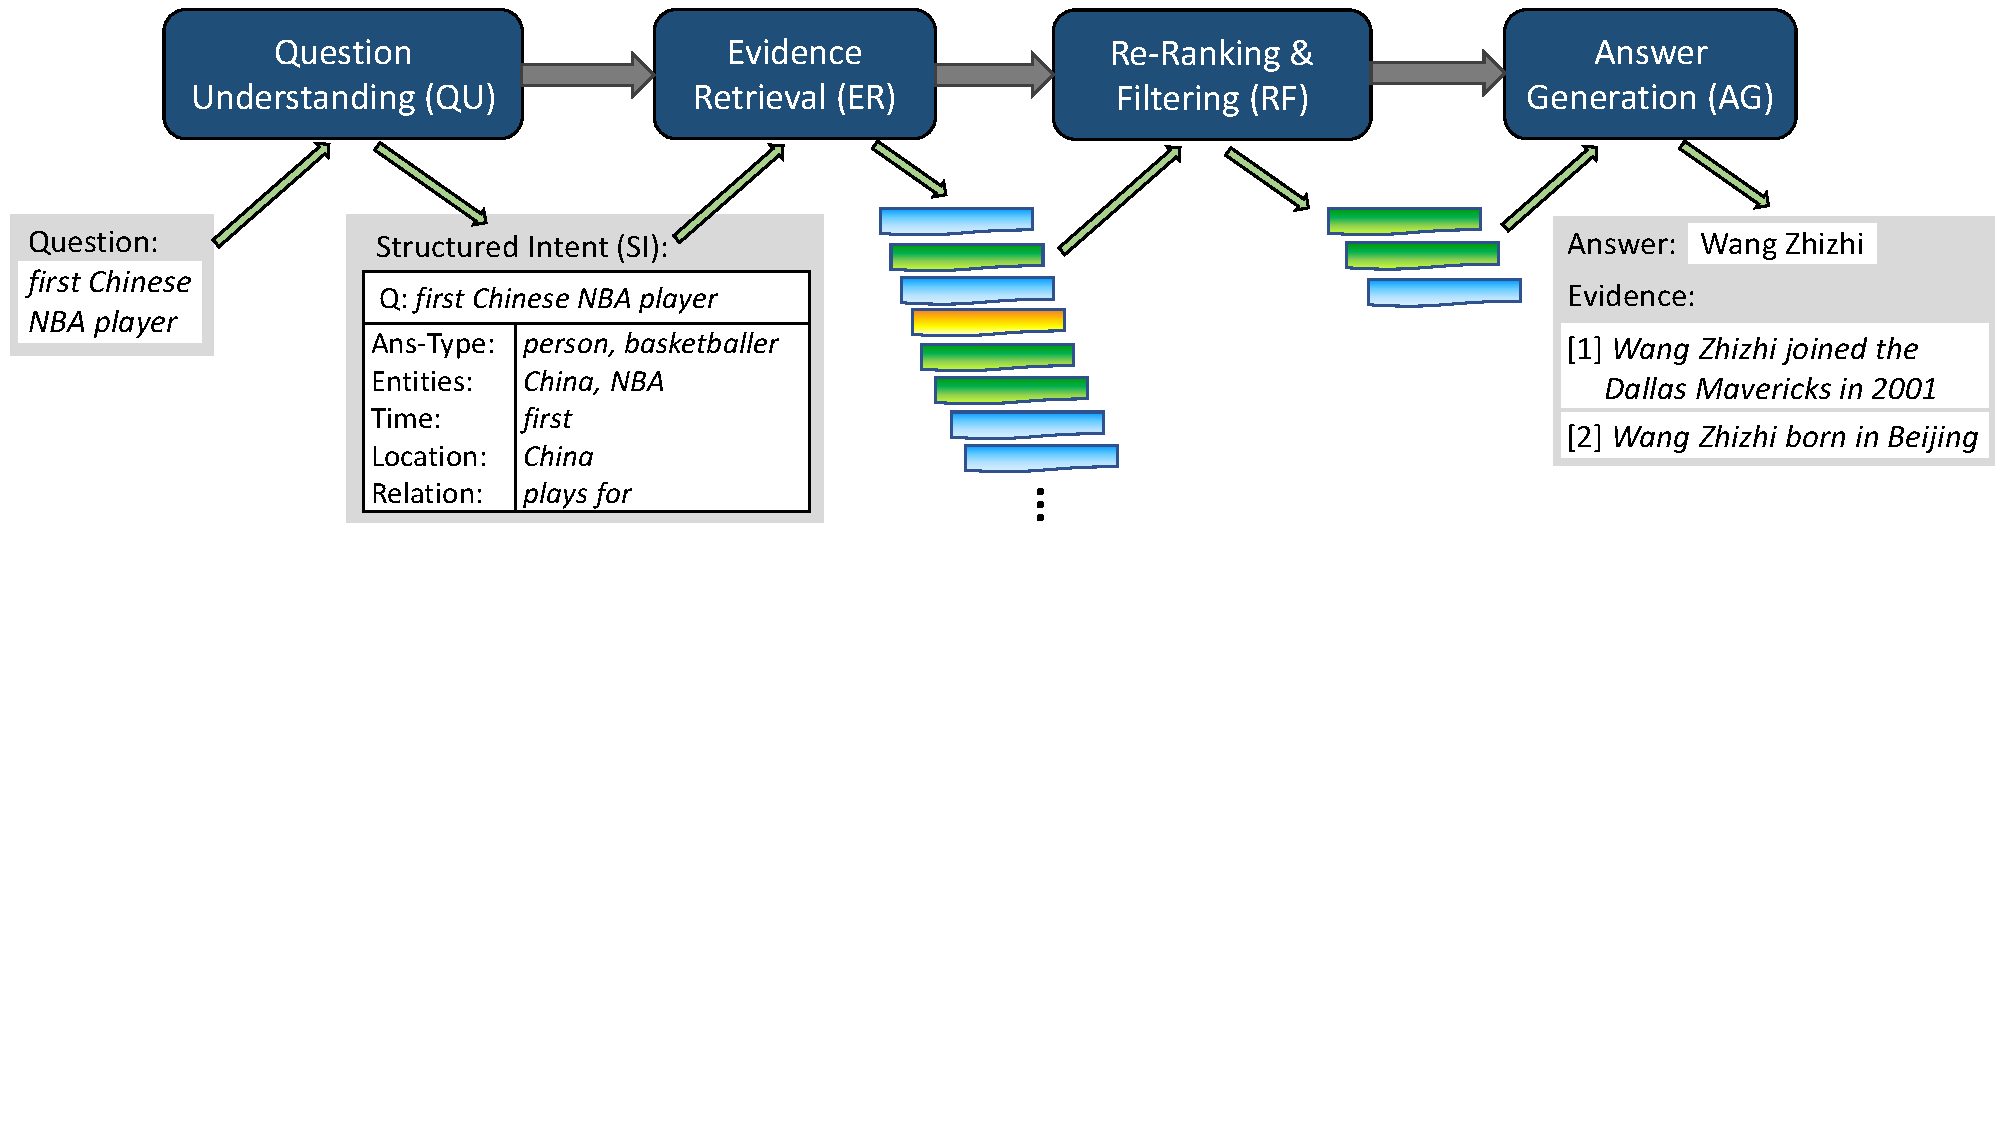
\includegraphics[width=\textwidth]{submissions/Gerhard2024/figures/compass-overview.pdf}
  \caption{Overview of the \method system.}
  \label{fig:compass-overview}
\end{figure}

% start with system overview
The \method system is a pipeline of four major stages, as illustrated in Figure \ref{fig:compass-overview}.
First, the input question is analyzed and decomposed, in order to compute a {\em structured intent (SI)} representation that will pass on to the subsequent steps, along with the original question. Second, the SI is utilized to retrieve pieces of evidence from different sources: text, KG and tables. 
Third, this pool of potentially useful evidence is filtered down, with iterative re-ranking, to arrive at a tractably small set of most promising evidence.
The final stage generates the answer from this evidence,
passing back the answer as well as evidence snippets for user-comprehensible explanation.

The second and fourth stage, Evidence Retrieval (ER) and Answer Generation (AG), are fairly standard. Such a two-phase architecture was called a retriever-reader architecture~\cite{Zhu-ODQA-survey:arxiv2021}. With a modern LLM replacing the earlier kinds of neural readers, this is the core of every RAG system~\cite{DBLP:journals/arXiv/abs-2312-10997}.

Stages 1 and 3 are unique elements of our architecture, judiciously introduced to improve both effectiveness (i.e., answer quality) and efficiency (i.e., computational cost).
Question Understanding (QU) provides the ER component with crisper and semantically refined input, and
the Re-Ranking \& Filtering (RF) stage is beneficial for
distilling the best evidence from the large pool of retrieved pieces.
The following subsections elaborate on the four stages of the pipeline, emphasizing the \method-specific steps QU and RF.



\subsection{Question Understanding (QU)}

% one par introducing the SI
To prepare the retrieval from different kinds of sources, including a KG, ad-hoc tables and text documents, it is useful to analyze and decompose the user question.
In this work, we aim to cast a question into a 
{\em structured intent (SI)} representation: essentially
a frame with faceted cues as slots, or equivalently, a concise set of key-value pairs. 
Figure \ref{fig:compass-overview} gives an idealized example for the question about the first Chinese NBA player. The facets or keys of potential interest here 
are:
\squishlist
\item {\em Ans-Type:} the expected answer type (or types when considering
different levels of semantic refinement), 
\item {\em Entities:} the salient entities in the question, and 
\item {\em Relation:} phrases that indicate which relation (between Q and A entities) the user is interested in. 
\squishend
\noindent In addition, as questions can have temporal or spatial aspects, the SI also foresees slots for:
\squishlist
\item {\em Time:} cues about answer-relevant time points or spans, including relative cues (e.g., ``before Covid'') and ordinal cues (e.g., ``first''), and
\item {\em Location:} cues about answer-relevant geo-locations.
\squishend

% discuss the spectrum of different SIs
\vspace{0.2cm}
\noindent The ideal SI for example question Q2 would look like:

\begin{quote}
{\em Ans-Type:} person, basketballer; {\em Entities:} China, NBA; {\em Time:} first;
{\em Location:} China; {\em Relation:} plays for.
\end{quote}

Note that the values for these slots can be crisp like entity names or dates, but they can also take the form of surface phrases. The SI purpose and value lie in the decomposition. In practice, many questions would only lead to a subset of faceted cues, leaving some slots empty. For the example in Figure \ref{fig:compass-overview}, an alternative SI could simply consist of

\begin{quote}
{\em Ans-Type:} person; {\em Entities:} China, NBA; {\em Time:} first.
\end{quote}

\noindent Even this simplified SI can be highly beneficial in guiding the subsequent evidence retrieval.

% sketch how an LM is trained to generate SIs 
To generate the SI from a user question, we employ a (small-scale) LM, specifically BART~\cite{DBLP:conf/acl/LewisLGGMLSZ20}, a Transformer-based auto-encoder with 140M parameters.\footnote{\url{https://huggingface.co/facebook/bart-base}}
BART is pre-trained for language representation; its power for our purpose comes from fine-tuning.
To this end, we generate (question, SI) pairs by using an instruction-trained LLM like GPT-4, with few-shot in-context learning (following our earlier work~\cite{Jia-FAITH:WWW2024}). 
Note that this is a one-time action; at inference-time we only use much smaller LMs.
The generated silver-standard pairs are then used to fine-tune BART.
In the experiments in this article, we leverage pre-existing collections of silver pairs, based on the training data of the CompMix benchmark~\cite{Christmann-CompMix:WWW2024}, 
comprising $3{,}400$ such pairs.


% outline value of SI for conversations
Although this paper focuses on single-shot questions, the \method architecture is also geared for conversational QA. In that setting, the SI can play an even bigger role, as (follow-up) questions are often formulated in a rather sloppy manner -- all but self-contained. For example, a conversation could start with a clear question {\em When did Wang Zhizhi join the NBA?}, followed a few dialog steps later, by a user utterance like {\em Which teams did he play for?} or simply {\em Which teams?}.
In such an informal conversation, the system needs to {\em contextualize} each user utterance based on the preceding turns in the dialog (e.g., inferring the relevant entities Wang Zhizhi and NBA from the conversational history).
For details on conversational QA, based on our architecture, see our earlier works~\cite{Christmann-CONVINSE:SIGIR2022,Christmann-Explaignn:SIGIR2023}.







%%%%%%%%%%%%%%%%%%%%%%%%%%%%%%%%%%%%%
\subsection{Evidence Retrieval (ER)}

The ER stage taps into a knowledge graph, a corpus of text documents, and a collection of web tables.
Specifically, for the experiments, we use the Wikidata KG,
all English Wikipedia articles, and all tables that are embedded in Wikipedia pages (incl. infoboxes, which can be seen as a special case of tables). 

% specifics: Clocq etc. - and the role of the SI
\vspace{0.2cm}
\noindent{\bf Retrieval from KG:}
To retrieve evidence from the KG, we utilize our earlier work
\clocq~\cite{Christmann-CLOCQ:WSDM2022}, which provides entity disambiguations and a relevant KG-subgraph for a given query.
Unlike most other works on QA-over-KG, \clocq fetches all KG-facts that are relevant for a given entity in a single step.
For example, when querying for
NBA players, it can traverse the KG neighborhood and pick up top teams, also considering so-called qualifier nodes in Wikidata which are often used for temporal scopes. 
As the disambiguation of entity names onto the KG can be tricky and noisy (e.g., China could be mapped to Chinese sports teams in all kinds of sports), \clocq considers several possible disambiguations~\cite{Christmann-CLOCQ:WSDM2022} (typically in the order of $10$ result entities).
The queries for \clocq are 
constructed by concatenating all slots of the question's SI.
For the example query about the first Chinese NBA player,
good result entities would be Dallas Mavericks, lists about NBA seasons, MVP awards etc., and their associated facts. These provide cues, but are likely insufficient to answer the question.


\vspace{0.2cm}
\noindent{\bf Retrieval from Text and Tables:}
The disambiguated entities returned by \clocq form anchors for tapping into text and tables.
\method first identifies 
relevant text documents and tables that refer to the anchor entities. With focus on Wikipedia, these are simply the articles for the respective entities. 
\method then constructs a keyword query that concatenates all available fields of the SI.
The query is evaluated against a linearized and verbalized representation (see below) of all sentences and all table rows in the selected documents.
This returns a set of sentences and 
and individual table rows, ranked by BM25 scores.


\vspace{0.2cm}
\noindent{\bf Evidence Verbalization:}
All results from the different data sources are uniformly treated by {\em linearizing} and {\em verbalizing} them
into token sequences. For KG results, the entity-centric triple sets are linearized via breadth-first traversal of the mini-graph starting from the entity node.
For tables, results are individual rows, which are contextualized by including labels from column headers and from the DOM-tree path of the article where the table comes from. For example, a table row about Wang Zhizhi playing for Dallas (Mavericks) in the 2000-2001 season, would be expressed as:

\vspace{0.05cm}
\hspace*{0.5cm} Wang Zhizhi / NBA Career / Season: 2000-2001, Team: Dallas, Games Played: 5 \dots
\vspace{0.05cm}

\noindent Finally, results from the text corpus are already in the form of token sequences, but we can additionally prefix these with the DOM-tree labels.
We can think of this entire pool of evidence as 
an on-the-fly corpus of potentially relevant pseudo-sentences, forming the input of the subsequent RF stage.


\vspace{0.2cm}
\noindent {\bf Result Ranking:}
Overall, the ER stage compiles a substantial set of evidence, possibly many thousands of entities, text snippets and table rows. Therefore, we practically restrict the pool to a subset of high-scoring pieces, like the top-$1000$.
For scoring, a simple BM25 model (a classical IR method) is applied. 
By default, we treat all evidence pieces uniformly with global scoring, no matter whether they come from KG, text or tables. 


\subsection{Re-Ranking and Filtering (RF)}

With a pool of top-$1000$ evidence pieces, we could invoke an LLM for answer generation. However, that would face a large fraction of noise (i.e., misleading evidence) and incur high costs of computation and energy consumption. 

For both of these reasons, we have devised light-weight techniques for iteratively reducing the top-$1000$ pieces to a small subset, say top-$30$ or top-$10$, that can be fed into an LLM at much lower cost (as LLM computations and pricing are at least linear in the number of input tokens). The difficulty is, of course, to do this without losing good evidence and reducing answer presence. Our techniques for this task are based on graph neural networks (GNNs)~\cite{Wu:IEEE2021} or cross-encoders (CEs)~\cite{Dejean:arxiv2024,Lin:MC2021}.

\myparagraph{GNN-based RF}
Given a large pool of evidence pieces from all sources, a bipartite graph is constructed:
\squishlist
\item {\em nodes} being evidence pieces or entities that occur in these pieces, and
\item {\em edges} connecting an evidence piece and an entity if the entity occurs in the evidence.
\squishend


The task for the GNN is to jointly score the evidence and the entity nodes in a multi-task learning setup. The latter are the {\em answer candidates}, and the evidence should give {\em faithful explanation} for an answer.
We build on our earlier work on explainable QA~\cite{Christmann-Explaignn:SIGIR2023}.

The node encodings are initialized with cross-encoder embeddings (see below) 
for node contents and the SI of the question. The inference iteratively adjusts the encodings based on message passing from neighboring nodes.
The GNN is trained via weak supervision from question-answer pairs:
evidence nodes are labeled as relevant if they are connected to
a gold answer.
More technical details are given in~\cite{Christmann-Explaignn:SIGIR2023}.

\method invokes the GNN in multiple rounds, iteratively reducing top-$k$ to top-$k^*$ nodes with $k^* \ll k$. In practice, we would typically consider two rounds: re-ranking top-$1000$ and pruning to top-100, and then reducing to top-30 or top-10, which are passed to the answer generation stage.
Note that this keeps the GNN at a tightly controlled size, so that its computational costs at inference-time are much smaller than those of an LLM.


\myparagraph{CE-based RF}
An alternative to the GNN inference is to employ a cross-encoder for scoring and re-ranking the evidence pieces.
These are transformers (typically with a small LM like BERT) that are fine-tuned for scoring the relatedness between a query and a document~\cite{Nogueira:arxiv2019}. In our case, the comparison is between the question SI and the evidence piece. In our experiments, we make use of two different cross-encoders, 
both trained on the MS-MARCO benchmark for passage retrieval~\cite{Bajaj:arxiv2018}, 
and fine-tuned on the respective benchmark (leveraging the same weak supervision data as for the GNNs),
the difference being in model size.\footnote{\url{https://huggingface.co/cross-encoder/ms-marco-MiniLM-L-4-v2} and\\ \url{https://huggingface.co/cross-encoder/ms-marco-MiniLM-L-6-v2}}
We use the smaller model to reduce top-$1000$ to top-100, and the larger model to go further down from top-100 to top-30.




%%%%%%%%%%%%%%%%%%%%%%%%%%%%%%%%%%%%%

\subsection{Answer Generation (AG)}

The last stage follows mainstream practice to invoke an LLM in a retrieval-augmented manner.
We call a `small-scale` LLM, specifically a fine-tuned LlaMA-3.1 model (8B-Instruct)\footnote{\url{https://huggingface.co/meta-llama/Llama-3.1-8B-Instruct}}, with a prompt \footnote{The specific prompt is \phrase{SI: \textless\texttt{concatenated SI}\textgreater \hspace{0.1cm} Evidence: \textless\texttt{evidence pieces}\textgreater}.}
consisting of:

\squishlist
\item the concatenated SI of the original question, and
\item the top-30 (or other top-$k^*$ with small $k^*$) evidence pieces.
\squishend

By the previous down-filtering of the original pool of evidence pieces, this last step has affordable cost in terms of computation time and energy consumption.

\vspace{0.2cm}
\noindent{\bf Fine-Tuning the LLM:}
We considered adding an instruction to the prompting, such as {\em ``answer this question solely based on the provided evidence snippets''}.
However, this turned out to be ineffective.
The reason why the model works well without such instructions is our task-specific fine-tuning.
We perform this by running the training data of benchmarks through the \method pipeline,
and training the AG stage with the top-30 evidence pieces as input.
Thus, the fine-tuning makes the model learn the role of evidence for RAG-based QA.

\vspace{0.2cm}
\noindent{\bf Explanations:}
The top-30 evidence pieces can be used to provide users with explanation of answers.
Optionally, these could be reduced further for comprehensibility.
Alternatively, we can fine-tune the LLM to provide both answers and concise explanations.
Since we can infer which evidences in the input mention the annotated ground-truth answers,
our method could be fine-tuned to provide such \textit{answering evidences} as well (cf.~\cite{Gao-citations:emnlp2023}).

\label{sec:exp}
\section{Experiments}


\label{setup}
\subsection{Experimental setup}


%%% BENCHMARKS
\myparagraphnospace{Benchmarks} We run experiments on three benchmarks with different characteristics of questions.

\squishlist
    \item \textbf{\compmix}.
    \compmix~\cite{Christmann-CompMix:WWW2024} is a benchmark which was specifically designed for evaluating QA systems operating over heterogeneous sources. The dataset has $9{,}410$ questions, out of which $2{,}764$ are used for testing.
    Answers are crisp entity names, dates, or other literals.
    
    \item \textbf{\crag}.
    We further evaluate on a subset of the \crag~\cite{Yang-CRAG} dataset, which was recently released as a testbed for RAG-based QA systems.
    We utilize the same pipeline and sources as outlined in Section~\ref{sec:method}, without using the web snippets or APIs provided with \crag. This way we focus on entity-centric questions that do not require access to live web data (e.g., news feeds), and disregard cases where the results would be up-to-date quantities.
    This restricts the test data to $436$ entity-centric questions, still enough for a proof of concept.
    
    \item \textbf{\timequestions}.
    To showcase the generalizability of our pipeline, we conduct experiments on~\timequestions~\cite{Jia-TimeQuestions},
    a benchmark for temporal QA. The dataset requires temporal understanding and reasoning, which are well-known limitations of
    LLMs~\cite{Dhingra-time-aware-LLM:TACL2022}. \timequestions has 16{,}181 questions (3{,}237 for testing).
\squishend

Typical examples for the questions in these three benchmarks are:

\begin{quote}
\compmix: \utterance{Which player won the most number of Man-of-the-Match titles in the FIFA world cup of 2006?}\\
 \indent \crag: \utterance{What was the worldwide box office sales for little hercules?}\\ 
  \indent \timequestions: \utterance{Which club did Cristiano Ronaldo play for before joining Real Madrid?}
\end{quote}

%%% BASELINES
\myparagraph{Baselines} As competitors or reference points to \method, we study the performance of the following methods:

\squishlist
    \item \textbf{Generative LLMs}.
    We compare \method against out-of-the-box LLMs: \textbf{\gptthree} (\texttt{text-davinci-003}), \textbf{\gptfour} (\texttt{gpt-4}) 
    and \textbf{\llama} (\texttt{meta-llama/Llama-3.1-8B-Instruct}).
    The same prompt is used for all LLMs, consistent with previous work~\cite{Christmann-CompMix:WWW2024, Zhang-Spaghetti:ACL2024}:
    \phrase{Please answer the following question by providing the crisp answer entity, date, year, or numeric number. Q: \textless\texttt{question}\textgreater}.
    

    \item \textbf{Heterogeneous QA methods}.
    \convinse~\cite{Christmann-CONVINSE:SIGIR2022}, \unikqa~\cite{Oguz-UniK-QA:NAACL2022}, \explaignn~\cite{Christmann-Explaignn:SIGIR2023}
    are QA methods designed to integrate heterogeneous sources: text, tables and KG. All of these  integrate the exact same sources as \method.

    
    \item \textbf{\textsc{State-of-the-art}}.
    For \compmix and \timequestions, we also compare against state-of-the-art methods from the literature: \spaghetti~\cite{Zhang-Spaghetti:ACL2024} and \textsc{Un-Faith}~\cite{Jia-FAITH:WWW2024}, which are among the best performing systems.
    
Results are taken from the literature whenever applicable.
On \crag, we use the models trained on \compmix for \method and heterogeneous QA baselines.
\squishend



%%% METRIC(S)
\myparagraph{Metrics}
We measure \textit{precision at 1} (\textbf{P@1}) as our main metric~\cite{RoyAnand:MC2021} on all benchmarks.
On \crag, we manually annotate answer correctness, as the ground-truth answer formats vary (e.g., entity name variants, lists, sentences).

We also compute the number of neural parameters aggregated over all sub-modules (\textbf{\#Parameters}).
Parameter counts for GPT-models are taken from~\cite{Minaee-LLM-survey}
(\gptfour might have less active parameters during inference).

For further analysis we measure \textit{answer presence} (\textbf{AP@k}),
i.e. whether the answer is present in the top-$k$ ranked evidence pieces,
and \textit{mean reciprocal rank} within the top-$k$ evidences (\textbf{MRR@k}).

%%% CONFIG
\myparagraph{Configuration}
Our implementation uses the \texttt{Llama3.1-8B-Instruct} model for the AG stage.
For the QU, ER and RF stages
we adopt code from the \explaignn project.\footnote{\url{https://explaignn.mpi-inf.mpg.de}}
For the ER stage, we use \clocq, setting its specific parameters to $k=10$ and $p=1{,}000$.

As default, we use the GNN technique for the RF stage.
For efficiency, we use light-weight models for initializing
the GNN encoders -- the same models used for the CE-based RF.\footnote{\url{https://huggingface.co/cross-encoder/ms-marco-MiniLM-L-4-v2} and\\\url{https://huggingface.co/cross-encoder/ms-marco-MiniLM-L-6-v2}}
The GNNs are trained for $5$ epochs with an epoch-wise evaluation strategy,
i.e. we choose the model with the best performance on the respective dev set.
We train the GNNs on graphs with a maximum of $100$ evidence and $400$ entity nodes (as scored by BM25).
During inference, the first GNN is applied on graphs with $1{,}000$ evidence and $4{,}000$ entity nodes, shrinking the pool of evidence pieces to the top-$100$.
The second GNN then runs on graphs with $100$ evidence and $400$ entity nodes.
The factor of 4 entities per evidence (on average) holds sufficient for the observed data,
and enables batched inference.
Other parameters are kept as is.

The AG model, based on \texttt{Llama3.1-8B-Instruct}, is 
fine-tuned
for $2$ epochs with a warm-up ratio of $0.01$ and a batch size of $8$, again with an epoch-wise evaluation strategy.
Other parameters are set to the default Hugging Face
training parameters.\footnote{\url{https://huggingface.co/docs/transformers/v4.46.2/en/main_classes/trainer\#transformers.TrainingArguments}}





\subsection{Main results}
%%% MAIN TABLE
\myparagraphnospace{\method is competitive on all benchmarks}
Main results of our experiments are shown in Table~\ref{tab:main-res}.
First of all, we note that \method achieves competitive performance across all three benchmarks.

On \compmix, baselines for heterogeneous QA and \llama perform similarly,
whereas GPT-based LLMs can answer more than $50$\% of the questions correctly.
\method exhibits substantially higher performance, on par with
the state-of-the-art method \textsc{Spaghetti}~\cite{Zhang-Spaghetti:ACL2024}
(which is based on \gptfour).

On the \crag dataset, P@1 drops for all methods except for \gptfour. 
The benchmark includes realistic questions,
which can be ambiguous/confusing (\phrase{who was the director for the report?}),
on ``exotic'' entities with answers in social media (\phrase{how many members does the teknoist have?}),
or require up-to-date information (\phrase{when did chris brown release a song or album the last time?}),
and other cases that are challenging for all methods.

Finally, \method establishes new state-of-the-art performance on the \timequestions benchmark.
Interestingly, all of the tested LLMs show greatly reduced performance on this benchmark,
which inherently requires temporal understanding and reasoning
-- a known weakness of stand-alone LLMs.


\begin{table} [h]
    \centering
    \newcolumntype{G}{>{\columncolor [gray] {0.90}}c}
    \begin{tabular}{l G G G c}
        \toprule
            \textbf{Method $\downarrow$ / Benchmark $\rightarrow$} & \textbf{\compmix}  & \textbf{\crag} & \textbf{\timequestions} & \textbf{\#Parameters} \\ 
        \midrule
            \textbf{\gptthree} 
            & $0.502$ &   $-$ & $0.224$ & $175{,}000$ M  \\
            % #params from https://arxiv.org/pdf/2402.06196

            \textbf{\gptfour}
            & $0.528$ &   $\mathbf{0.633}$ & $0.306$ & $1{,}760{,}000$ M \\
            % #params from https://arxiv.org/pdf/2402.06196

            \textbf{\llama~\cite{Touvron-LLaMA}} (8B-Instruct)
            & $0.431$ &   $0.385$ & $0.178$ & $8{,}030$ M  \\
            % #params from Huggingface (8,030,257,152)
        \midrule
            \textbf{\convinse~\cite{Christmann-CONVINSE:SIGIR2022}}
            & $0.407$  &   $0.298$ & $0.423$  & $362$ M \\
            % FiD: 222,903,936 + BART (SR-generation): 139,420,416 = 362,324,352 (python explaignn/question_understanding/structured_representation/get_num_params.py)

            \textbf{\unikqa~\cite{Oguz-UniK-QA:NAACL2022}}
            & $0.440$ &   $0.280$ & $0.424$ & $223$ M  \\
            % FiD: 222,903,936 (python explaignn/heterogeneous_answering/fid_module/FiD/get_num_params.py)
    
            \textbf{\explaignn~\cite{Christmann-Explaignn:SIGIR2023}} 
            & $0.442$ &   $0.303$ & $0.525$  & $328$ M \\
            % BART (SR-generation): 139,420,416 + 2GNNs: 94520832 + 93930240 = 327,871,488

        \midrule 
            \textbf{\textsc{State-of-the-art}}
            & $\mathbf{0.565}$ 
            & $-$
            & $0.571$  & $-$ \\

            & (\textsc{Spaghetti}~\cite{Zhang-Spaghetti:ACL2024})
            & 
            & (\textsc{Un-Faith}~\cite{Jia-FAITH:WWW2024}) &  \\

        \midrule
            \textbf{\method (ours)}
            & ${0.564}$ &   $0.362$ & $\mathbf{0.754}$  & $8{,}218$ M \\
            % BART (SR-generation): 139,420,416 + LLaMA: 8,030,257,152 + GNNs: 25,670,016 + 22,268,928 =  8,217,616,510
        \bottomrule
    \end{tabular} 
    \vspace*{-0.2cm}
    \caption{End-to-end P@1 of \method and baselines on three benchmarks. Results for \gptthree and \gptfour are taken from the literature~\cite{Christmann-CompMix:WWW2024, Jia-FAITH:WWW2024}. \gptthree is not accessible anymore, hence no results on \crag.
    }
    \label{tab:main-res}
\end{table}





%%% ANSWER SOURCES
\myparagraph{Integration of heterogeneous sources is vital}
\method integrates evidence from text, KG and tables into a unified framework.
We aim to better understand how this affects the answering performance of the method.
Table~\ref{tab:sources} shows end-to-end answering performance of \method
with different combinations of the input sources.
The results clearly indicate that all types of sources contribute, with option Text+KG+Tables performing best,
with a large margin over tapping only single source types.

\begin{table} [t] 
    \centering
    \newcolumntype{G}{>{\columncolor [gray] {0.90}}c}
    \newcolumntype{H}{>{\setbox0=\hbox\bgroup}c<{\egroup}@{}}
    	\begin{tabular}{l G G G H H H c c c} 
        \toprule
            \textbf{Benchmark $\rightarrow$}
                & \multicolumn{3}{G}{\textbf{\compmix}} 
                & \multicolumn{3}{H}{\textbf{\crag}}
                & \multicolumn{3}{c}{\textbf{\timequestions}} \\ 
        \midrule
            \textbf{Input sources $\downarrow$ / Metric $\rightarrow$}
                & \textbf{P@1} & \textbf{AP@100}  & \textbf{AP@30}
                & \textbf{P@1} & \textbf{AP@100}  & \textbf{AP@30}
                & \textbf{P@1} & \textbf{AP@100}  & \textbf{AP@30} \\
            \midrule
                \textbf{Text}           &  $0.455$  &  $0.563$  &  $0.531$ &  $?$  &  $?$  &  $?$ &  $0.539$  &  $0.515$  &  $0.487$   \\
                \textbf{KG}             &  $0.481$  &  $0.677$  &  $0.637$ &  $?$  &  $?$  &  $?$ &  $0.724$  &  $0.701$  &  $0.674$   \\
                \textbf{Tables}         &  $0.432$  &  $0.501$  &  $0.482$ &  $?$  &  $?$  &  $?$ &  $0.536$  &  $0.347$  &  $0.328$   \\
            \midrule
                \textbf{Text+KG}        &  $0.537$  &  $0.749$  &  $0.706$ &  $?$  &  $?$  &  $?$ &  $0.745$  &  $\mathbf{0.776}$  &  $0.748$   \\
                \textbf{Text+Tables}    &  $0.503$  &  $0.632$  &  $0.594$ &  $?$  &  $?$  &  $?$ &  $0.567$  &  $0.578$  &  $0.549$   \\
                \textbf{KG+Tables}      &  $0.524$  &  $0.728$  &  $0.692$ &  $?$  &  $?$  &  $?$ &  $ 0.743$  &  $0.731$  &  $0.703$   \\
            \midrule
                \textbf{Text+KG+Tables}    &  $\mathbf{0.564}$  &  $\mathbf{0.759}$  &  $\mathbf{0.724}$ &  $?$ &  $?$  &  $?$ & $\mathbf{0.754}$    & $\mathbf{0.776}$  &  $\mathbf{0.749}$   \\
            \bottomrule
    \end{tabular}
    \vspace*{-0.2cm}
    \caption{Answer presence and answering precision of \method with different combinations of input sources (on the respective test sets).}
    \label{tab:sources}
\end{table}




\subsection{Analysis}

%%% TOP-K vs. 3xTOP-(K/3)
\myparagraph{Unified retrieval enhances performance}
In the RF stage, we re-rank and filter evidence from different source types,
and feed the unified top-\textit{k}* into the AG stage.
We conduct a comparison in which we consider
the top-$10$ evidence pieces from each source type individually. This gives equal influence to KG, text and tables, whereas our default is based on global ranking.
Table~\ref{tab:unified-retrieval} shows the results for this analysis, showing our default choice performs better.
The reason is that different questions require different amounts of evidence from each of the source types.

\begin{table} [t] 
    \centering
    \newcolumntype{G}{>{\columncolor [gray] {0.90}}c}
    \newcolumntype{H}{>{\setbox0=\hbox\bgroup}c<{\egroup}@{}}
    	\begin{tabular}{l G G H H} 
        \toprule
            \textbf{Input evidences $\downarrow$ / Metric $\rightarrow$} & \textbf{P@1} & \textbf{AP@30}  & \textbf{\crag} & \textbf{\timequestions} \\ 
            \midrule
                \textbf{Top-30 Text+KG+Tables (ours)}             &  $\mathbf{0.574}$  &  $\mathbf{0.710}$  &  $-$  &  $-$   \\
                \textbf{Top-10 Text + Top-10 KG + Top-10 Tables}        &  $0.560$    &  $0.709$  &  $-$  &  $-$   \\
            \bottomrule
    \end{tabular}
    \vspace*{-0.2cm}
    \caption{Answer presence and precision
    of \method for different choices of top-30 
    (on \compmix dev set).}
    \label{tab:unified-retrieval}
\end{table}


%%% NUMBER OF EVIDENCES
\myparagraph{\method works well with small amounts of evidence}
We investigate the 
influence of 
the number of evidence pieces
fed into the AG stage, varying it from $5$ to $100$.
Results are shown in Figure~\ref{fig:res-num-evidences}.
As the curve shows, there is a sharp increase in precision as we add evidence up to 30 or 40 pieces, which is around our default of top-30. This indicates that a certain amount of evidence is needed, to overcome the inherent noise and arrive at sufficient answer presence. 
As we increase the amount of evidence further, we observe a saturation effect, and eventually a degration of performance. Too much evidence not only has diminishing returns, but can actually be confusing for the AG stage. This reconfirms our heuristic choice of top-30: enough for good answering while keeping computational costs reasonably low.


\begin{figure}[t]
    \centering
    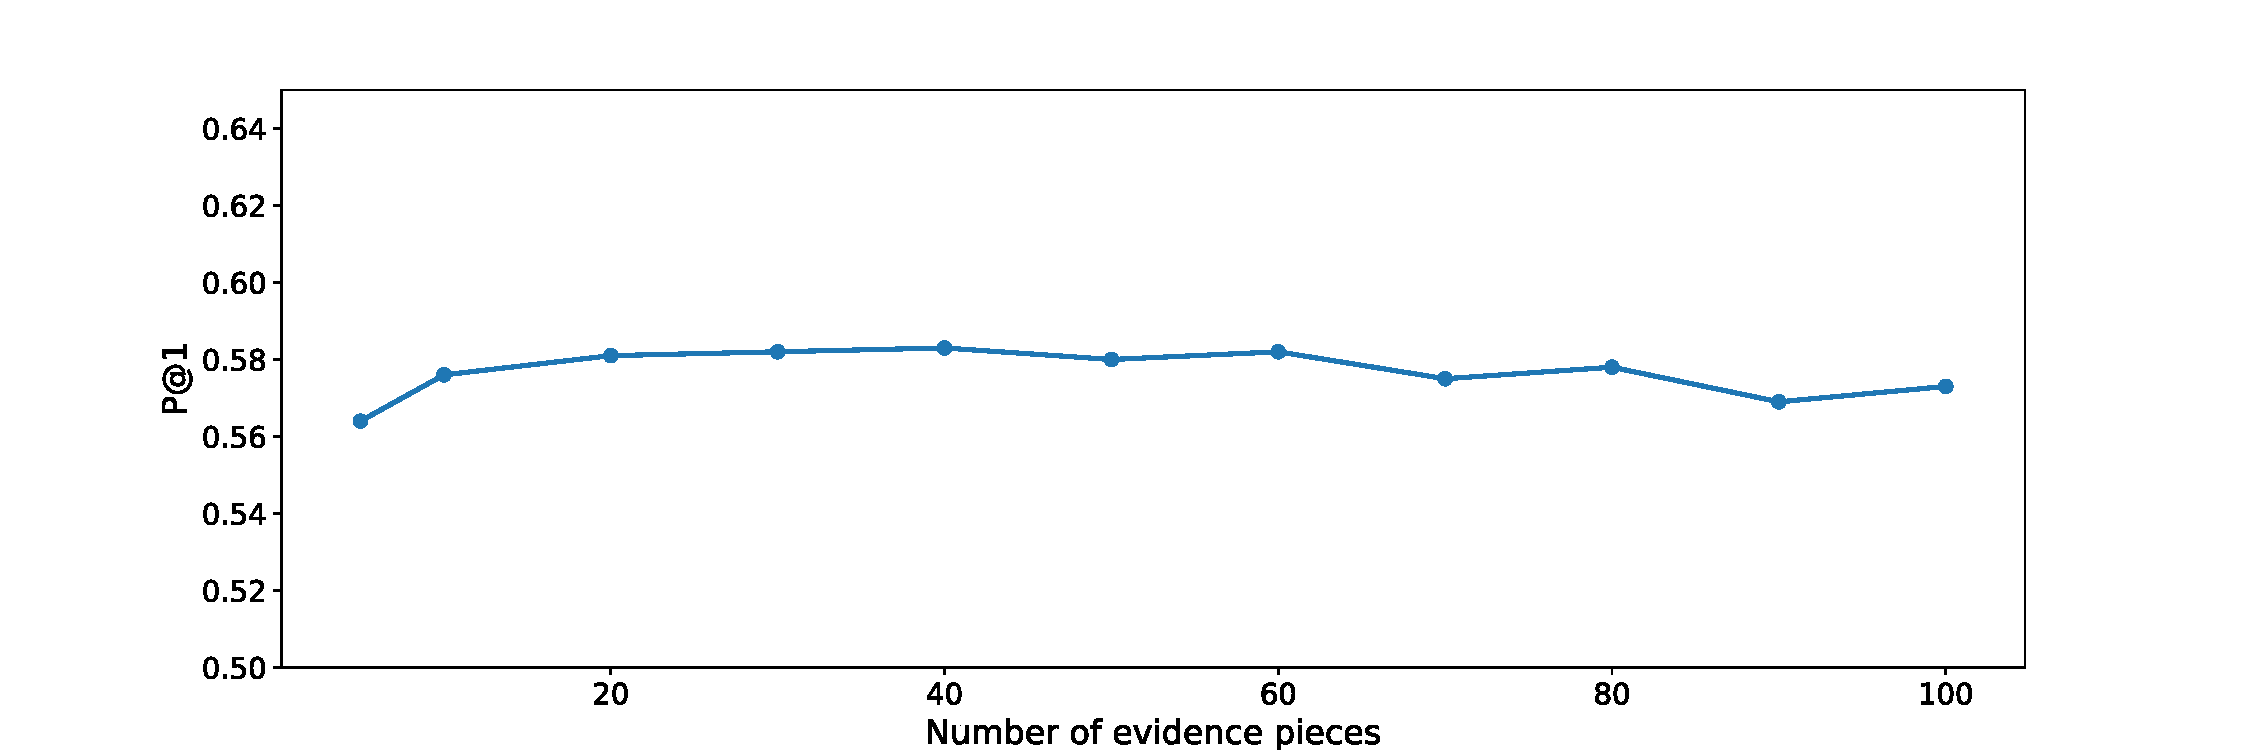
\includegraphics[width=0.8\textwidth]{submissions/Gerhard2024/figures/p_at_1-line_with_evidences.pdf}
    \vspace*{-0.2cm}
    \caption{Performance of \method on the \compmix dev set with different numbers of evidence.}
    \label{fig:res-num-evidences}
    \vspace*{-0.2cm}
\end{figure}



%%% ABLATION
\myparagraph{Ablation study on re-ranking} For more insight on the possible configurations of the RF stage, we conducted an ablation study with different options, including solely relying on the initial BM25 scoring without explicit re-ranking. The results are shown in Table \ref{tab:ablation2}. We observe that the iterative reduction in two steps is slightly better than the single-step variants (going down from top-1000 to top-30 in one RF step). Between the two options of using a GNN or a CE, the differences are negligible. A notable effect is that our RF techniques retain the answer presence at a very high level, only a bit lower than for the initial top-1000. 
The last two rows of Table \ref{tab:ablation2} demonstrate that RF is crucial: without explicit re-ranking, the technique of just picking smaller top-$k$ from the original BM25 model leads to substantial degradation in both answer presence and precision. 


\begin{table} [t] \small
    \centering
    \newcolumntype{G}{>{\columncolor [gray] {0.90}}c}
    \newcolumntype{H}{>{\setbox0=\hbox\bgroup}c<{\egroup}@{}}
    	\begin{tabular}{l G H G G G} 
        \toprule
            & \multicolumn{5}{G}{\textbf{\compmix} (dev set)} \\
        \midrule
            \textbf{RF Method $\downarrow$ / Metric $\rightarrow$} & \textbf{P@1} & \textbf{AP@1000} & \textbf{AP@100}  & \textbf{AP@30} & \textbf{MRR@100} \\ 
        \midrule
            \textbf{GNN: 1000 $\rightarrow$ 100 $\rightarrow$ 30}             &  $\mathbf{0.574}$  & $0.760$ &  $0.738$  &  $0.710$  &  $\mathbf{0.572}$  \\
            \textbf{CE: 1000 $\rightarrow$ 100 $\rightarrow$ 30}          &  $0.573$  & $0.760$  &   $\mathbf{0.740}$ &  $\mathbf{0.721}$   &  $0.553$   \\
        \midrule
            \textbf{GNN: 1000 $\rightarrow$ 30} &  $0.567$  & $?$  &   $n/a$ &  $0.710$   &  $0.567$   \\
         \textbf{CE: 1000 $\rightarrow$ 30} &  $0.570$  & $0.760$  &   $n/a$ &  $0.715$   &  $0.558$   \\
            \midrule
           \textbf{BM25: 100 (w/o GNN or CE)} &  $0.490$ & $0.760$  &  $0.652$  &  $n/a$  &  $0.259$ \\       
            \textbf{BM25: 30 (w/o GNN or CE)} &  $0.468$  & $0.760$  &  $n/a$ &  $0.534$   &  $0.259$   \\
            \bottomrule
    \end{tabular}
    \vspace*{-0.2cm}
    \caption{Ablation study for different RF strategies of \method on the \compmix dev set. The answer presence in the RF input with top-$1000$ evidence pieces is $0.760$.}
    \label{tab:ablation2}
\end{table}



\myparagraph{Quality of SI}
To assess the quality and robustness of the Structured Intents, we
inspected a sample of questions and their SIs.
Table~\ref{tab:question-SI-examples} gives three anecdotic examples.
We show SIs generated by \method, which makes use of the pre-existing collection from the \compmix benchmark for training.
This training data was obtained via different heuristics, 
which can be a limiting factor when user intents become more complex.

Therefore, we also looked at SIs derived via in-context learning (ICL) using \gptfour with $5$ handcrafted examples.
As shown in our earlier work on temporal QA~\cite{Jia-FAITH:WWW2024},
such data can be used for training smaller models (e.g., BART),
which can greatly boost the completeness and overall quality of the generated SIs.

From the sampled set, we observed that the ICL-based SIs are more
complete with all slots filled, whereas the BART-based SIs focused more
on the main slots Answer-type, Entities and Relation.
However, both approaches achieve very high quality in filling the slots,
capturing the user's information need very well.

Interestingly, when questions get complicated, with nested phrases, 
the ICL-based variant succeeds in decomposing the questions, based on only $5$ ICL examples.
For example, for the question {\em ``which German state had the most Corona-related death cases in the first year after the outbreak?''}
the Time slot becomes {\em ``first year after Corona outbreak''},
which can be resolved to identify the temporal scope.
In general, we believe that such question decomposition, beyond simple temporal constraints,
would be an interesting theme for future work.

\begin{table} [t] 
    \centering
    \small
    \newcolumntype{G}{>{\columncolor [gray] {0.90}}c}
    \newcolumntype{H}{>{\setbox0=\hbox\bgroup}c<{\egroup}@{}}
    \resizebox*{\textwidth}{!}{
        \begin{tabular}{p{6cm}|p{6cm}|p{6cm}} 
        \toprule
            \textbf{Question} & \textbf{Current SI by \method} & \textbf{SI via ICL} \\
        \midrule
        \textit{what was disneys first color movie?}
            & Ans-Type: \textit{animated feature film} & Ans-Type: \textit{film, animated film} \\
            & Entities: \textit{disneys} & Entities: \textit{Disney} \\
            & Relation: \textit{was first color movie} & Relation: \textit{first color movie} \\
            &  & Time: \textit{first} \\
        \midrule
        \textit{at the oscars, who won best actor in 2018?}
            & Ans-Type: \textit{human} & Ans-Type: \textit{person, actor} \\
            & Entities: \textit{at the oscars} & Entities: \textit{Oscars, 2018} \\
            & Relation: \textit{who won best actor in 2018} & Relation: \textit{won best actor} \\
            &  & Time: \textit{2018} \\
        \midrule
        \textit{which German state had the most Corona-} & Ans-Type: \textit{state} & Ans-Type: \textit{location, state} \\
        \textit{related death cases in the first year after} & Entities: \textit{Germany, Corona} & Entities: \textit{Germany, Corona-related deaths} \\
        \textit{the outbreak?} & Relation: \textit{which state had the most related} & Relation: \textit{highest count of death cases} \\
        & \textit{death cases in the first year after the out-}  & Location: \textit{Germany} \\
            & \textit{break}  & Time: \textit{first year after Corona outbreak} \\
        \bottomrule
    \end{tabular}
    }
    \vspace*{-0.2cm}
    \caption{Examples for pairs of question and generated SI.}
    \label{tab:question-SI-examples}
\end{table}




%%% REFRAIN FROM ANSWER
\myparagraph{Refraining from answering}
%%% Searched for: "generated_answer I" (with I being the full word, not partial) in the generated answers of LLaMA
%%% yields 245 results out of 2764 questions on CompMix
%%% yields 1270 results out of 3237 questions on TimeQuestions
We can train our model to refrain from answering in scenarios
where the provided evidence does not contain an answer to the question.
Specifically, during training, when the answer is not present in the evidence,
we change the target answer to {\em unknown}. This variant is referred to as \method {\em (faithful)}.

We measure the ratio of questions for which {\em unknown} is provided as answer,
and the P@1 restricted to questions that are answered.
The accuracy of refraining from answering is measured as well,
based on whether the answer is present in the evidence or not.
We conduct this experiment on \compmix and \timequestions,
for which we can compute answer presence exactly.
We also compute results for \llama, which is already instructed 
with the option to answer ``don't know''.
Table~\ref{tab:refrain-from-answer} shows the results.
For \compmix, we observe that \method has high accuracy on refraining when appropriate,
whereas \llama tends to be overconfident with a very small rate of {\em unknowns}, leading to incorrect answers.

\begin{table} [t] \small
    \centering
    \newcolumntype{G}{>{\columncolor [gray] {0.90}}c}
    \newcolumntype{H}{>{\setbox0=\hbox\bgroup}c<{\egroup}@{}}
    	\begin{tabular}{l G G G G c c c c} 
        \toprule
            & \multicolumn{4}{G}{\textbf{\compmix}} & \multicolumn{4}{c}{\textbf{\timequestions}} \\
            \midrule
            \textbf{Metric $\rightarrow$} & \textbf{P@1}  & \textbf{P@1} & \textbf{Refrain} & \textbf{Refrain} & \textbf{P@1}  & \textbf{P@1} & \textbf{Refrain} & \textbf{Refrain} \\ 
            \textbf{Method $\downarrow$} &                 & \textbf{(answered)} & \textbf{rate} & \textbf{accuracy} &                 & \textbf{(answered)} & \textbf{rate} & \textbf{accuracy} \\ 
            \midrule
                \textbf{\llama}             &  $0.431$  &  $0.471$  &  $0.089$  &  $n/a$  &  $0.177$  &  $0.276$  &  $0.392$  &  $n/a$  \\
                \textbf{\method (faithful)}           &  $0.497$  &  $0.713$  &  $0.303$  &  $0.838$ &  $0.597$  &  $0.804$  &  $0.257$  &  $0.864$  \\
            \bottomrule
    \end{tabular}
    \vspace*{-0.2cm}
    \caption{
        Performance of \method with option to refrain from answering (``don't know'').
    }
    \label{tab:refrain-from-answer}
\end{table}

\label{sec:disc}
\section{Insights, Limitations, and Challenges}


\noindent{\bf Benchmark Performance.} Our method, RAG-based \method with an 8B LLaMA model, outperforms much larger LLMs like \gptfour on two of the three benchmarks, with a very large margin for temporal questions. Obviously, pre-trained LLMs have only limited sense of properly positioning ``remembered’’ facts on the timeline even with training data that exceeds ours by several orders of magnitude. This confirms our intuition that LLMs alone are not good at ``recalling’’  higher-arity relations that require combining distant pieces of evidence. This is a sweet spot for RAG. Only for 
the \crag benchmark, \method is substantially inferior to a full-blown LLM. This is likely due to the nature of the questions: not necessarily the complexity of the information needs, but the need for more web sources (beyond what our experiments tap into).

\vspace{0.2cm}
\noindent{\bf Cost/Performance Ratio.} The most important take-away from our experiments is that \method achieves its competitive performance at a much lower cost than the full LLMs. Assuming that the consumed GFlops are proportional to the number of model parameters, \method achieves a cost reduction by a factor of 200x for \gptthree and 2000x for \gptfour. This does not only mean less computation, but also a massively lower electricity bill and climate impact.  

\vspace{0.2cm}
\noindent{\bf Role of Question Understanding.} We did not systematically investigate the influence of the Structured Intent in the \method pipeline. However, the comparison to the big GPT models reflects the role of the SI, as we prompt the GPT models in their natural mode with the original questions. The linearized sequence of available SI slots does not always have major advantages, but there are enough cases where specific facets provide crucial cues. This holds especially for the Entities slot, as this drives the gathering of evidence in the ER stage (cf.~\cite{Christmann-CONVINSE:SIGIR2022}, and for the Time slot, as these cues are often decisive for temporal questions (cf.~\cite{Jia-FAITH:WWW2024}).

\vspace{0.2cm}
\noindent{\bf Role of Re-Ranking.} As our ablation studies show, merely using top-$k$ evidence from an initial BM25-style ranking does not provide good performance. Also, there seems to be sweet spot in the choice of $k$: we need enough evidence for connecting the dots if the question requires multiple pieces of information, or for corroborating candidates if the question finds many useful but noisy pieces. In the experiments, $k=30$ turns out to be good choice; much lower $k$ results in insufficient evidence, and much larger $k$ leads to saturation and ultimately degrading performance. Our argument for iteratively shrinking the candidate set in multiple rounds of re-ranking is substantiated in our experiments, but the gain of doing this, compared to GNN- or CE-based re-ranking from 1000 to 30, is not big. More research is called to better understand the role of ranking in RAG. 

\vspace{0.2cm}
\noindent{\bf Limitations of Evidence Retrieval.}
For ER, we adopted more or less standard techniques. The results showed very good answer presence, in the order of 75\% in the top-100 or even top-30. An important case where this is insufficient are questions that require aggregating information over a large number of evidence pieces. An example is asking for the life-time total of 3-point scores of the basketball player Dirk Nowitzki.
This requires collecting a set of per-season tables with NBA player statistics, but also other web sources with numbers for his career before he joined the NBA (including his youth teams).
Of course, there are sometimes shortcuts like a Wikipedia article or biography mentioning the total number, but this cannot be universally assumed. The bottom line is that ER should be reconsidered as well, striving to improve the recall dimension.

\vspace{0.2cm}
\noindent{\bf Limitations of Answer Generation.}
For AG, we simply rely on a LLM,
using it as an extractor (``reader'') from the given evidence. Despite the wide belief that LLMs can perform deep
reasoning over many pieces of evidence, our experience is that the extraction works only well – robustly and faithfully – for relatively simple questions with a few multi-hop joins or simple aggregation over a few pieces. However, complicated questions such as asking for the top-100 NBA players with the largest number of life-time 3-point scores (again including their pre-NBA careers) are currently out of scope and will likely remain so for quite some time. This offers many opportunities for pushing the envelope further.

\vspace{0.2cm}
\noindent{\bf Trust in Data Sources.}
In our experiments, we considered all heterogeneous sources as trustworthy and unbiased. With focus on Wikidata and Wikipedia, this assumption has been well justified. In the wild, however, input data for RAG-based systems likely exhibit a wide spectrum of quality issues, in terms of stale information, biased positions, or simply false statements. Identifying trustworthy and up-to-date evidence and dealing with conflicting data, has been explored in other contexts (e.g., for KG curation~\cite{Dong-Trust:PVLDB2015}), but remains a major challenge for RAG-based QA.


\vspace{0.2cm}
\noindent{\bf Open Challenges and Future Work.} The best-performing methods in our experiment, mostly \method, reach P@1 values of 56\% for \compmix and 75\% for \timequestions. 
For the latter, the answer presence in the top-100 is only slightly higher; so the AG stage hardly misses anything.
However, for \compmix, the answer presence is 75\% -- much higher than what our system can actually answer. Obviously, closing this gap is a major direction to pursue, with focus on the RF and AG stages. However, missing one fourth of the answers completely in the top-100 pool, is a big problem as well. This requires improving recall at the ER stage, possibly with better guidance by the QU, which in turn needs more sources beyond the scope of our experiments (currently limited to Wikidata and Wikipedia). 

In general, we need to think beyond this kind of ``benchmark mindset’’. Even if we reached 80\% or 90\% precision and recall, we would still have a substantial fraction of questions that are answered incorrectly
or not at all. 
The remaining errors may not be a problem for chatbots, but they would be a showstopper for the deployment of mission-critical applications in business or science. We believe that this big gap is a shortcoming of {\em all methods}, not an issue that comes from the data alone. For trivia-style QA, as looked at in this paper, a smart human in ``open book’’ mode and no time limitation should be able to properly answer practically all questions, just by reading pieces of web contents and putting things together. Neither LLMs nor state-of-the-art RAG are the final solution; substantial research and creative ideas are needed to further advance QA.


\clearpage
\newpage

\newcommand{\bibauthors}[1]{{#1}}
\newcommand{\bibtitle}[1]{\emph{#1}}
\newcommand{\bibconf}[1]{{#1}}

\begin{thebibliography}{10}

\bibitem{Bajaj:arxiv2018}
\bibauthors{Payal Bajaj, Daniel Campos, Nick Craswell, Li Deng, Jianfeng Gao, Xiaodong Liu, Rangan Majumder, Andrew McNamara, Bhaskar Mitra, Tri Nguyen, Mir Rosenberg, Xia Song, Alina Stoica, Saurabh Tiwary, Tong Wang.}
\bibtitle{MS MARCO: A Human Generated MAchine Reading COmprehension Dataset.}
In \bibconf{arXiv 2018}.

\bibitem{DBLP:conf/acl/ChenFWB17}
\bibauthors{Danqi Chen, Adam Fisch, Jason Weston and Antoine Bordes.}
\bibtitle{Reading Wikipedia to Answer Open-Domain Questions.}
In \bibconf{ACL 2017}.

\bibitem{Christmann-CONVINSE:SIGIR2022}
\bibauthors{Philipp Christmann, Rishiraj Saha Roy, Gerhard Weikum.}
\bibtitle{Conversational Question Answering on Heterogeneous Sources.}
In \bibconf{SIGIR 2022}.

\bibitem{Christmann-CLOCQ:WSDM2022}
\bibauthors{Philipp Christmann, Rishiraj Saha Roy, Gerhard Weikum.}
\bibtitle{Beyond NED: Fast and Effective Search Space Reduction for Complex Question Answering over Knowledge Bases.}
In \bibconf{WSDM 2022}.

\bibitem{Christmann-Explaignn:SIGIR2023}
\bibauthors{Philipp Christmann, Rishiraj Saha Roy, Gerhard Weikum.}
\bibtitle{Explainable Conversational Question Answering over Heterogeneous Sources via Iterative Graph Neural Networks.}
In \bibconf{SIGIR 2023}.

\bibitem{Christmann-CompMix:WWW2024}
\bibauthors{Philipp Christmann, Rishiraj Saha Roy, Gerhard Weikum.}
\bibtitle{CompMix: A Benchmark for Heterogeneous Question Answering.}
In \bibconf{WWW 2024}.

\bibitem{Dejean:arxiv2024}
\bibauthors{Herve Dejean, Stephane Clinchant, Thibault Formal.}
\bibtitle{A Thorough Comparison of Cross-Encoders and LLMs for Reranking SPLADE.}
In \bibconf{arXiv 2024}.

\bibitem{Dhingra-time-aware-LLM:TACL2022}
\bibauthors{Bhuwan Dhingra, Jeremy R Cole, Julian Martin Eisenschlos, Daniel Gillick, Jacob Eisenstein, and William W Cohen.}
\bibtitle{Time-Aware Language Models as Temporal Knowledge Bases.}
In \bibconf{TACL 2022}.

\bibitem{Dong-Trust:PVLDB2015}
\bibauthors{Xin Luna Dong, Evgeniy Gabrilovich, Kevin Murphy, Van Dang, Wilko Horn, Camillo Lugaresi, Shaohua Sun, Wei Zhang.}
\bibtitle{Knowledge-Based Trust: Estimating the Trustworthiness of Web Sources.}
In \bibconf{PVLDB 2015}.

\bibitem{DBLP:journals/arXiv/abs-2312-10997}
\bibauthors{Yunfan Gao, Yun Xiong, Xinyu Gao, Kangxiang Jia, Jinliu Pan, Yuxi Bi, Yi Dai, Jiawei Sun, Qianyu Guo, Meng Wang, Haofen Wang.}
\bibtitle{Retrieval-Augmented Generation for Large Language Models: A Survey.}
In \bibconf{arXiv 2023}.

\bibitem{Gao-citations:emnlp2023}
\bibauthors{Tianyu Gao, Howard Yen, Jiatong Yu, Danqi Chen.}
\bibtitle{Enabling Large Language Models to Generate Text with Citations.}
In \bibconf{EMNLP 2023}.

\bibitem{Guu-REALM:ICML2020}
\bibauthors{Kelvin Guu, Kenton Lee, Zora Tung, Panupong Pasupat, Ming-Wei Chang.}
\bibtitle{Retrieval Augmented Language Model Pre-Training.}
In \bibconf{ICML 2020}.

\bibitem{DBLP:conf/eacl/IzacardG21}
\bibauthors{Gautier Izacard, Edouard Grave.}
\bibtitle{Leveraging Passage Retrieval with Generative Models for Open Domain Question Answering.}
In \bibconf{EACL 2021}.

\bibitem{Jia-TimeQuestions}
\bibauthors{Zhen Jia, Soumajit Pramanik, Rishiraj Saha Roy, and Gerhard Weikum.}
\bibtitle{Complex Temporal Question Answering on Knowledge Graphs.}
In \bibconf{CIKM 2021}.

\bibitem{Jia-FAITH:WWW2024}
\bibauthors{Zhen Jia, Philipp Christmann, Gerhard Weikum.}
\bibtitle{Faithful Temporal Question Answering over Heterogeneous Sources.}
In \bibconf{WWW 2024}.

\bibitem{DBLP:journals/arXiv/abs-2305-06984}
\bibauthors{Ehsan Kamalloo, Nouha Dziri, Charles L. A. Clarke, Davood Rafiei.}
\bibtitle{Evaluating Open-Domain Question Answering in the Era of Large Language Models.}
In \bibconf{arXiv 2023}.

\bibitem{Kandpal:ICML2023}
\bibauthors{Nikhil Kandpal, Haikang Deng, Adam Roberts, Eric Wallace, Colin Raffel.}
\bibtitle{Large Language Models Struggle to Learn Long-Tail Knowledge.}
In \bibconf{ICML 2023}.

\bibitem{DBLP:conf/emnlp/KarpukhinOMLWEC20}
\bibauthors{Vladimir Karpukhin, Barlas Oguz, Sewon Min, Patrick S. H. Lewis, Ledell Wu, Sergey Edunov, Danqi Chen, Wen-tau Yih.}
\bibtitle{Dense Passage Retrieval for Open-Domain Question Answering.}
In \bibconf{EMNLP 2020}.

\bibitem{Lee-MATTER:ACL2024}
\bibauthors{Dongkyu Lee, Chandana Satya Prakash, Jack FitzGerald, Jens Lehmann.}
\bibtitle{MATTER: Memory-Augmented Transformer Using Heterogeneous Knowledge Sources.}
In \bibconf{ACL 2024}.

\bibitem{DBLP:conf/acl/LewisLGGMLSZ20}
\bibauthors{Mike Lewis, Yinhan Liu, Naman Goyal, Marjan Ghazvininejad, Abdelrahman Mohamed, Omer Levy, Veselin Stoyanov, Luke Zettlemoyer.}
\bibtitle{BART: Denoising Sequence-to-Sequence Pre-training for Natural Language Generation, Translation, and Comprehension.}
In \bibconf{ACL 2020}.

\bibitem{DBLP:conf/nips/LewisPPPKGKLYR020}
\bibauthors{Patrick S. H. Lewis, Ethan Perez, Aleksandra Piktus, Fabio Petroni, Vladimir Karpukhin, Naman Goyal, Heinrich Küttler, Mike Lewis, Wen-tau Yih, Tim Rocktäschel, Sebastian Riedel, Douwe Kiela.}
\bibtitle{Retrieval-Augmented Generation for Knowledge-Intensive NLP Tasks.}
In \bibconf{NeurIPS 2020}.

\bibitem{Lin:MC2021}
\bibauthors{Jimmy Lin, Rodrigo Frassetto Nogueira, Andrew Yates.}
\bibtitle{Pretrained Transformers for Text Ranking: BERT and Beyond.}
In \bibconf{Morgan \& Claypool Publishers 2021}.

\bibitem{Liu-SUQL:NAACL2024}
\bibauthors{Shicheng Liu, Jialiang Xu, Wesley Tjangnaka, Sina J. Semnani, Chen Jie Yu, Monica Lam.}
\bibtitle{SUQL: Conversational Search over Structured and Unstructured Data with Large Language Models.}
In \bibconf{NAACL-HLT 2024}.

\bibitem{Mavi:FnT2024}
\bibauthors{Vaibhav Mavi, Anubhav Jangra, Adam Jatowt.}
\bibtitle{Multi-hop Question Answering.}
In \bibconf{Foundations and Trends in Information Retrieval 2024}.

\bibitem{Minaee-LLM-survey}
\bibauthors{Shervin Minaee, Tomas Mikolov, Narjes Nikzad, Meysam Chenaghlu, Richard}
\bibtitle{Socher, Xavier Amatriain, and Jianfeng Gao.}
Large Language Models: A Survey.
In \bibconf{arXiv 2024}.

\bibitem{Nogueira:arxiv2019}
\bibauthors{Rodrigo Frassetto Nogueira, Kyunghyun Cho.}
\bibtitle{Passage Re-ranking with BERT.}
In \bibconf{arXiv 2019}.

\bibitem{Oguz-UniK-QA:NAACL2022}
\bibauthors{Barlas Oguz, Xilun Chen, Vladimir Karpukhin, Stan Peshterliev, Dmytro Okhonko, Michael Sejr Schlichtkrull, Sonal Gupta, Yashar Mehdad, Scott Yih.}
\bibtitle{UniK-QA: Unified Representations of Structured and Unstructured Knowledge for Open-Domain Question Answering.}
In \bibconf{NAACL-HLT 2022}.

\bibitem{RogersGA:CS2023}
\bibauthors{Anna Rogers, Matt Gardner, Isabelle Augenstein.}
\bibtitle{QA Dataset Explosion: A Taxonomy of NLP Resources for Question Answering and Reading Comprehension.}
In \bibconf{ACM Computing Surveys 2023}.

\bibitem{RoyAnand:MC2021}
\bibauthors{Rishiraj Saha Roy, Avishek Anand.}
\bibtitle{Question Answering for the Curated Web: Tasks and Methods in QA over Knowledge Bases and Text Collections.}
In \bibconf{Synthesis Lectures on Information Concepts, Retrieval, and Services, Morgan \& Claypool Publishers 2021}.

\bibitem{Pramanik-Uniqorn:JWS2024}
\bibauthors{Soumajit Pramanik, Jesujoba Alabi, Rishiraj Saha Roy, Gerhard Weikum.}
\bibtitle{UNIQORN: Unified Question Answering over RDF Knowledge Graphs and Natural Language Text.}
In \bibconf{Journal of Web Semantics 2024}.

\bibitem{Sun-PullNet:EMNLP2019}
\bibauthors{Haitian Sun, Tania Bedrax-Weiss, William W. Cohen.}
\bibtitle{PullNet: Open Domain Question Answering with Iterative Retrieval on Knowledge Bases and Text.}
In \bibconf{EMNLP/IJCNLP 2019}.

\bibitem{Sun:NAACL2024}
\bibauthors{Kai Sun, Yifan Ethan Xu, Hanwen Zha, Yue Liu, Xin Luna Dong.}
\bibtitle{Head-to-Tail: How Knowledgeable are Large Language Models (LLMs)? A.K.A. Will LLMs Replace Knowledge Graphs?}
In \bibconf{NAACL-HLT 2024}.

\bibitem{Touvron-LLaMA}
\bibauthors{Hugo Touvron, Thibaut Lavril, Gautier Izacard, Xavier Martinet, Marie-Anne Lachaux, Timothée Lacroix, Baptiste Rozière, Naman Goyal, Eric Hambro, Faisal Azhar, Aurelien Rodriguez, Armand Joulin, Edouard Grave, Guillaume Lample.}
\bibtitle{Llama: Open and efficient foundation language models.}
In \bibconf{arXiv 2023}.

\bibitem{Wu-STARK:arxiv2024}
\bibauthors{Shirley Wu, Shiyu Zhao, Michihiro Yasunaga, Kexin Huang, Kaidi Cao, Qian Huang, Vassilis N. Ioannidis, Karthik Subbian, James Zou, Jure Leskovec.}
\bibtitle{STaRK: Benchmarking LLM Retrieval on Textual and Relational Knowledge Bases.}
In \bibconf{arXiv 2024}.

\bibitem{Wu:IEEE2021}
\bibauthors{Zonghan Wu, Shirui Pan, Fengwen Chen, Guodong Long, Chengqi Zhang, Philip S. Yu.}
\bibtitle{A Comprehensive Survey on Graph Neural Networks.}
In \bibconf{IEEE Transactions on Neural Networks and Learning Systems 2021}.

\bibitem{Yang-CRAG}
\bibauthors{Xiao Yang, Kai Sun, Hao Xin, Yushi Sun, Nikita Bhalla, Xiangsen Chen, Sajal Choudhary, Rongze D. Gui, Ziran W. Jiang, Ziyu Jiang, Lingkun Kong, Brian Moran, Jiaqi Wang, Yifan Ethan Xu, An Yan, Chenyu Yang, Eting Yuan, Hanwen Zha, Nan Tang, Lei Chen, Nicolas Scheffer, Yue Liu, Nirav Shah, Rakesh Wanga, Anuj Kumar, Wen-tau Yih, Xin Luna Dong.}
\bibtitle{CRAG -- Comprehensive RAG Benchmark.}
In \bibconf{arXiv 2024}.

\bibitem{Yasunaga:NAACL2021}
\bibauthors{Michihiro Yasunaga, Hongyu Ren, Antoine Bosselut, Percy Liang, Jure Leskovec.}
\bibtitle{QA-GNN: Reasoning with Language Models and Knowledge Graphs for Question Answering.}
In \bibconf{NAACL-HLT 2021}.

\bibitem{Zhang-Spaghetti:ACL2024}
\bibauthors{Heidi C. Zhang, Sina J. Semnani, Farhad Ghassemi, Jialiang Xu, Shicheng Liu, Monica S. Lam.}
\bibtitle{SPAGHETTI: Open-Domain Question Answering from Heterogeneous Data Sources with Retrieval and Semantic Parsing.}
In \bibconf{ACL 2024}.

\bibitem{Zhang:NAACL2024}
\bibauthors{Jiahao Zhang, Haiyang Zhang, Dongmei Zhang, Yong Liu, Shen Huang.}
\bibtitle{End-to-End Beam Retrieval for Multi-Hop Question Answering.}
In \bibconf{NAACL-HLT 2024}.

\bibitem{Zhao-LLMsurvey}
\bibauthors{Wayne Xin Zhao, Kun Zhou, Junyi Li, Tianyi Tang, Xiaolei Wang, Yupeng Hou, Yingqian Min, Beichen Zhang, Junjie Zhang, Zican Dong, Yifan Du, Chen Yang, Yushuo Chen, Zhipeng Chen, Jinhao Jiang, Ruiyang Ren, Yifan Li, Xinyu Tang, Zikang Liu, Peiyu Liu, Jian-Yun Nie, Ji-Rong Wen.}
\bibtitle{A Survey of Large Language Models.}
In \bibconf{arXiv 2023}.

\bibitem{Zhao:arxiv2024}
\bibauthors{Penghao Zhao, Hailin Zhang, Qinhan Yu, Zhengren Wang, Yunteng Geng, Fangcheng Fu, Ling Yang, Wentao Zhang, Bin Cui.}
\bibtitle{Retrieval-Augmented Generation for AI-Generated Content: A Survey.}
In \bibconf{arXiv 2024}.

\bibitem{Zhu-ODQA-survey:arxiv2021}
\bibauthors{Fengbin Zhu, Wenqiang Lei, Chao Wang, Jianming Zheng, Soujanya Poria, Tat-Seng Chua.}
\bibtitle{Retrieving and Reading: A Comprehensive Survey on Open-domain Question Answering.}
In \bibconf{arXiv 2021}.

\end{thebibliography}


\end{document}

\end{article}

\begin{article}
{Evaluating the Factuality of Large Language Models using Large-Scale Knowledge Graphs}
{Xiaoze Liu, Feijie Wu, Tianyang Xu, Zhuo Chen, Yichi Zhang, Xiaoqian Wang, Jing Gao}
\setcounter{section}{0}
\NeedsTeXFormat{LaTeX2e} 
\ProvidesPackage{debulletin}[2002/04/01 Data Engineering Bulletin package]
% \RequirePackage{epsfig}

%%%%%%%%%%%%%%%%%%%%%%%%%%%%%%%%%%%%%%%%%%%%%%%%%%%%%%%%%%%%%%%%%%%%%%%%
%%
%% INTRODUCTION
%%
%%%%%%%%%%%%%%%%%%%%%%%%%%%%%%%%%%%%%%%%%%%%%%%%%%%%%%%%%%%%%%%%%%%%%%%%
% 
% This is a LaTeX package for the Bulletin of the Technical Community on
% Data Engineering.  It is intended to be used with the article document
% class at 11pt, but it can probably be used with report and book classes
% and other font sizes as well.
% The expected format of the bulletin is
% 
% 1. A cover.  This includes:
%    - a front cover page with the title, date, volume, and number of 
%      the issue, and with the table of contents
%    - an inside cover page giving the names of the editors and committee 
%      members, and other information
%    - an inside back cover that is blank
%    - a back cover that is blank, except for the IEEE mailing address and
%      the postage permit just below the fold half way down the page.
% 2. A few miscellaneous columns, probably from the editor of the special
%    issue and an overview of the area covered by the special issue.
% 3. A few letters to the editor.
% 4. The contributed articles
% 5. A few calls for papers for coming conference.
% 
% An example of how such an issue is as follows.
% Note that there are several formatting paramters, and they are described
% at the end of this file.
%
%%%%%%%%%%%%%%%%%%%%%%%%%%%%%%%%%%%%%%%%%%%%%%%%%%%%%%%%%%%%%%%%%%%%%%%%
%
% \documentclass[11pt]{article}
% \usepackage{debulletin}
% \begin{document}
% 
% \bulletindate{March 2002}
% \bulletinvolume{1}
% \bulletinnumber{1}
% \bulletinyear{2002}
% \begin{bulletin}
% 
% %
% %  Introductory columns.  In table of contents, we want a heading 
% %  ``Introduction'' followed by subheadings (that is, table of contents 
% %  subentries) for each of the two columns.  Inside the bulletin, we
% %  want each column preceded by a heading giving the title of the column.
% %
% \tocheading{Introduction}
% 
% \heading{A letter from the Editor}
% \tocsubentry{A letter from the Editor}{I. M. Editor}
% \input{editorletter}
% 
% \heading{Easy-to-use Databases: a Tutorial}
% \tocsubentry{Easy-to-use Databases: a Tutorial}{I. M. Expert}
% \input{tutorial}
% 
% %
% %  Letters to the editor section.  Use the lettersection environment.
% %  Each letter is contained in a letter environment, where the two required
% %  options to \begin{letter} are the author and the address of the author.
% %
% \begin{lettersection}
% 
% \begin{letter}{My database is better than yours}{D. B. Hacker}%
% 					{Hacker, Inc. \\ Cambridge, MA}
% \input{dbhacker}
% \end{letter}
% 
% \begin{letter}{No it isn't}{Betty D. Hacker}{Betty, Inc. \\ Palo Alto, CA}
% \input{bdhacker}
% \end{letter}
% 
% \end{lettersection}
% 
% %
% %  Contributed articles section.  Use the articlesection environment.
% %  The argument to the articlesection command is TOPIC, where the name
% %  of the special issue is supposed to be ``Special Issue on TOPIC''.
% %  Each article is contained in an article environment, where the two 
% %  required options to \begin{article} are the title and author of 
% %  the article.
% %
% \begin{articlesection}{Easy-to-Use Databases}
% 
% \begin{article}{Easy Data Entry}{David Crowbar}
% \input{crowbar}
% \end{article}
% 
% \begin{article}{Data Security made Simple}{General Confusion}
% \input{confusion}
% \end{article}
% 
% \end{articlesection}
% 
% %
% %  Calls for papers section.  Use the callsection environment.
% %  Each call for papers is contained in an call environment, where the single 
% %  required options to \begin{call} is the name of the conference.
% %
% \begin{callsection}
% \begin{call}{DB Conference A}
% \input{dba}
% \end{call}
% 
% \begin{call}{DB Conference B}
% \input{dbb}
% \end{call}
% \end{callsection}
% 
% \end{bulletin}
% \end{document}
%
%%%%%%%%%%%%%%%%%%%%%%%%%%%%%%%%%%%%%%%%%%%%%%%%%%%%%%%%%%%%%%%%%%%%%%%%

%%%%%%%%%%%%%%%%%%%%%%%%%%%%%%%%%%%%%%%%%%%%%%%%%%%%%%%%%%%%%%%%%%%%%%%%
% 
% The bulletin environment.
% 
% The bulletin environment generates the covers.  The two sides of the
% front cover are generated by \begin{bulletin}, and the two sides of
% the back cover are generated by \end{bulletin}.
%
%%%%%%%%%%%%%%%%%%%%%%%%%%%%%%%%%%%%%%%%%%%%%%%%%%%%%%%%%%%%%%%%%%%%%%%%

\newenvironment{bulletin}%
  {\@MakeCoverOne\@MakeCoverTwo}%
  {\cleardoublepage
   \@MakeCoverThree\@MakeCoverFour
  }
%
% The outside front cover
%
\newcommand{\@MakeCoverOne}{
  \begingroup
    \@SetCoverDimensions
    \begin{titlepage}
      \thispagestyle{empty}
      %\vbox{}\vskip .5in
      \textbf{\Large Bulletin of the Technical Community on}
      \par\bigskip
      \textbf{\@namefontsize Data}
      \par\medskip
      \textbf{\@namefontsize Engineering}
      \par\bigskip
      \textbf{\Large \@BulletinDate \quad Vol. \@BulletinVolume{} No. 
        \@BulletinNumber \hfill \@includeIEEElogo IEEE Computer Society}
      \par\bigskip
      \hrule
      \par
%      \bigskip
      \tableofcontents
      \vfil
    \end{titlepage}
  \endgroup
}
\newcommand{\@BulletinDate}{June 2018}
\newcommand{\@BulletinNumber}{2}
\newcommand{\@BulletinVolume}{41}
\newcommand{\@BulletinYear}{2018}
\newcommand{\bulletindate}[1]{\renewcommand{\@BulletinDate}{#1}} 
\newcommand{\bulletinnumber}[1]{\renewcommand{\@BulletinNumber}{#1}}
\newcommand{\bulletinvolume}[1]{\renewcommand{\@BulletinVolume}{#1}}
\newcommand{\bulletinyear}[1]{\renewcommand{\@BulletinYear}{#1}}

%
% The inside front cover
% 
\newcommand{\@MakeCoverTwo}{
  \begingroup
    \@SetCoverDimensions
    \@includeinsidefront 
  \endgroup
}
%
% The inside back cover
% 
\newcommand{\@MakeCoverThree}{
  \begingroup
    \@SetCoverDimensions
    \@includeinsideback 
  \endgroup
}
%
% The outside back cover
% 
\newcommand{\@MakeCoverFour}{
  \begingroup
    \@SetCoverDimensions
    \begin{titlepage}
      \thispagestyle{empty}
      \vbox{}\vskip .5\coverheight
      \hbox to \hsize{\@PrintIEEEAddress \hfill \@PrintPostagePermit}
      \vfil
    \end{titlepage}
  \endgroup
}
\newcommand{\@PrintIEEEAddress}{\hbox to 0pt{\vbox{\@IEEEAddress}\hss}}
\newcommand{\@PrintPostagePermit}{\hbox to 0pt{\hss\framebox{\hbox to 1.25in
  {\hss\vbox to 1.25in{\hsize 1.25in \center \vss \@PostagePermit \vss}}}}}
\newcommand{\@IEEEAddress}{}	  
\newcommand{\@PostagePermit}{}
\newcommand{\IEEEAddress}[1]{\renewcommand{\@IEEEAddress}{#1}} 
\newcommand{\PostagePermit}[1]{\renewcommand{\@PostagePermit}{#1}}  
%
% Compute cover layout dimentions
%
% Reset \oddsidemargin, \evensidemargin, and \topmargin so that the covers
% are centered on the physical page.
% The height and width of the physical page are determined by 
% \physicalpageheight and \physicalpagewidth.
% The height and width of text on the cover are determined by \coverheight
% and \coverwidth.
%
\newcommand{\@SetCoverDimensions}{%
  \hsize \coverwidth
  \oddsidemargin \physicalpagewidth
  \advance \oddsidemargin by -\coverwidth
  \divide \oddsidemargin by 2%
  \advance \oddsidemargin by -1in%
  \evensidemargin \oddsidemargin
  %
  \vsize \coverheight
  \topmargin \physicalpageheight
  \advance \topmargin by -\coverheight
  \divide \topmargin by 2%
  \advance \topmargin by -\topskip
  \advance \topmargin by -\headheight
  \advance \topmargin by -\headsep
  \advance \topmargin by -1in%
  %
  \parindent 0pt%
  \parskip   0pt%
}

%%%%%%%%%%%%%%%%%%%%%%%%%%%%%%%%%%%%%%%%%%%%%%%%%%%%%%%%%%%%%%%%%%%%%%%%%%
%
%  The LETTER SECTION.
%
% The section is enclosed between \begin{lettersection} and \end{lettersection}
% commands, and each letter is enclosed between 
% \begin{letter}{TITLE}{AUTHOR}{ADDRESS} and \end{letter} commands where
% TITLE and AUTHOR are the title and author of the letter and ADDRESS is
% the ADDRESS of the author (complete with \\ separating lines of the address
% as usual).
%
%%%%%%%%%%%%%%%%%%%%%%%%%%%%%%%%%%%%%%%%%%%%%%%%%%%%%%%%%%%%%%%%%%%%%%%%%%

\newenvironment{lettersection}%
       {\clearpage
%	\tocskip{\bigskipamount}
	\tocheading{\strut Letters}
	\tocskip{\smallskipamount}
	\pageheading{Letters}{Letters}
	\thispagestyle{plain}
	}%
       {\clearpage}
\newenvironment{letter}[3]
       {\newcommand{\lettertitle}{#1}
	\newcommand{\letterauthor}{#2}
	\newcommand{\letteraddress}{#3}
        	\tocsubentry{\lettertitle}{\letterauthor}
	\heading{\lettertitle}
	\makeatletter
        \@RestoreMaketitle
	\@UndefinePreambleCommands
	\NeedsTeXFormat{LaTeX2e}
\ProvidesPackage{deauthor}[2002/04/01 Data Engineering Bulletin Author package]

%
% Undefine the \date command, so no date is printed with the title
%
\renewcommand{\date}[1]{}
\renewcommand{\@date}{\@empty}

%
% Undefine the titlepage environment so that articles don't try to
% circumvent the journal's formatting conventions for the first page.
% This works for the article class, but causes trouble for reports and 
% books since the \maketitle command is defined in terms of the titlepage 
% environment.
%
\renewenvironment{titlepage}{}{}

%
% Undefine the \pagestyle and \thispagestyle commands so that articles
% don't try to change the page style.
%
\renewcommand{\pagestyle}[1]{}
\renewcommand{\thispagestyle}[1]{}

%
% Define common theorem-like environment created with the \newtheorem
% command.  First we have to undefine them all since we just defined them
% in the previous article.  Also, define a proof environment and a \qed
% symbol to end the proof.
%
% This initial hack redefines the theorem-like environments of latex to
% follow the theorem heading with a colon (e.g. Theorem 4:) and print
% the theorem text in roman font.
%
\renewcommand{\@begintheorem}[2]%
        {\trivlist \item[\hskip \labelsep{\bf #1\ #2:}]}
\renewcommand{\@opargbegintheorem}[3]%
        {\trivlist \item[\hskip \labelsep{\bf #1\ #2\ (#3):}]}
%
\let\theorem\relax
\let\lemma\relax
\let\corollary\relax
\let\proposition\relax
\let\claim\relax
\let\definition\relax
\let\proof\relax \let\endproof\relax
%
\newtheorem{theorem}{Theorem}
\newtheorem{lemma}[theorem]{Lemma}
\newtheorem{corollary}[theorem]{Corollary}
\newtheorem{proposition}[theorem]{Proposition}
\newtheorem{claim}[theorem]{Claim}
\newtheorem{definition}[theorem]{Definition}
%
\newenvironment{proof}{\noindent {\bf Proof:}}{}
\newcommand{\squarebox}[1]{\hbox to #1{\hfill\vbox to #1{\vfill}}}

%Modified from new command to renew command by Márton Balassi
\newcommand{\qed}{\hspace*{\fill}
            \vbox{\hrule\hbox{\vrule\squarebox{.667em}\vrule}\hrule}\smallskip}

%
% Define an example environment, just another theorem environment but with
% independent numbering.
%
\let\example\relax
\newtheorem{example}{Example}

%
% Define an indented abstract environment.
%
\renewenvironment{abstract}%
  {\begin{center}\textbf{Abstract}\end{center}\narrower\itshape}%
  {\par}  

%
% Reset all section and figure counters so that an article's section
% and figure numbers begin with 1.
%
\setcounter{section}{0}
\setcounter{figure}{0}


%
% Place page formatting parameters (like page dimensions) here
% These should match the dimensions in bulletin.sty.
%
\textheight     9.0in
\textwidth      6.75in
\oddsidemargin  0.0in
\evensidemargin -0.25in
\topmargin      0.0in
\headheight     0.0in
\headsep        0.0in
%\footheight     0.0in

\@twosidetrue        % print on two sides of a page

%
% Authors are not supposed to change page dimensions.
%

\let\@setlength\setlength       % save old definition
\renewcommand{\setlength}[2]{%
  \@VerifyChangeableLength{#1}%
  \if@ChangeableLength\@setlength{#1}{#2}\else\@UnchangeableError{#1}\fi}

\let\@addtolength\addtolength   % save old definition
\renewcommand{\addtolength}[2]{%
  \@VerifyChangeableLength{#1}%
  \if@ChangeableLength\@addtolength{#1}{#2}\else\@UnchangeableError{#1}\fi}

\let\@settowidth\settowidth     % save old definition
\renewcommand{\settowidth}[2]{%
  \@VerifyChangeableLength{#1}%
  \if@ChangeableLength\@settowidth{#1}{#2}\else\@UnchangeableError{#1}\fi}

\newif\if@ChangeableLength      \@ChangeableLengthtrue
\newcommand{\@VerifyChangeableLength}[1]{%
  \ifx#1\textwidth              \@ChangeableLengthfalse
  \else\ifx#1\textheight        \@ChangeableLengthfalse
  \else\ifx#1\textwidth         \@ChangeableLengthfalse
  \else\ifx#1\oddsidemargin     \@ChangeableLengthfalse
  \else\ifx#1\evensidemargin    \@ChangeableLengthfalse
  \else\ifx#1\topmargin         \@ChangeableLengthfalse
  \else\ifx#1\headheight        \@ChangeableLengthfalse
  \else\ifx#1\headsep           \@ChangeableLengthfalse
  \else\ifx#1\footheight        \@ChangeableLengthfalse
  \else\@ChangeableLengthtrue\fi\fi\fi\fi\fi\fi\fi\fi\fi}
\newcommand{\@UnchangeableError}[1]{%
  \errmessage{Error: Authors are not allowed to change #1.. Ignored}}

%
% We want the title to be typeset in boldface, and the author names
% to be typeset in italics.  We can hardwire this for the title,
% but trying to do the same thing for the author causes confusion
% due to the use of \@author in \@maketitle in article.sty.
% 
% We also want to print a copyright notice and the bulletin title at
% the bottom of every first page.
%
\renewcommand{\title}[1]{%
  \gdef\@title{\textbf{#1}}
  \begingroup 
  \renewcommand{\thefootnote}{\fnsymbol{footnote}}
  \global\setcounter{footnote}{0}
  \footnotetext{%
    \emph{Copyright {\@BulletinYear} IEEE. Personal use of this material is
    permitted. However, permission to reprint/republish this material for
    advertising or promotional purposes or for creating new collective
    works for resale or redistribution to servers or lists, or to reuse
    any copyrighted component of this work in other works must be obtained
    from the IEEE.}\\
    \textbf{Bulletin of the IEEE Computer Society Technical Committee on
    Data Engineering} \\
    \footnoterule
  }%
  \endgroup
}
\providecommand{\@BulletinYear}{2015}
\providecommand{\bulletinyear}[1]{\renewcommand{\@BulletinYear}{#1}}

  % read in the author style file
	\makeatother
	}%
       {\par\nobreak\vspace{\medskipamount}\noindent
             \vbox{\raggedleft\letterauthor\\
             \letteraddress 
             \par}\vskip 1in}
\newenvironment{kletter}[3]
       {\newcommand{\lettertitle}{#1}
	\newcommand{\letterauthor}{#2}
	\newcommand{\letteraddress}{#3}
        	\tocsubentry{\lettertitle}{\letterauthor}
	\heading{\lettertitle}
	\makeatletter
        \@RestoreMaketitle
	\@UndefinePreambleCommands
	\NeedsTeXFormat{LaTeX2e}
\ProvidesPackage{deauthor}[2002/04/01 Data Engineering Bulletin Author package]

%
% Undefine the \date command, so no date is printed with the title
%
\renewcommand{\date}[1]{}
\renewcommand{\@date}{\@empty}

%
% Undefine the titlepage environment so that articles don't try to
% circumvent the journal's formatting conventions for the first page.
% This works for the article class, but causes trouble for reports and 
% books since the \maketitle command is defined in terms of the titlepage 
% environment.
%
\renewenvironment{titlepage}{}{}

%
% Undefine the \pagestyle and \thispagestyle commands so that articles
% don't try to change the page style.
%
\renewcommand{\pagestyle}[1]{}
\renewcommand{\thispagestyle}[1]{}

%
% Define common theorem-like environment created with the \newtheorem
% command.  First we have to undefine them all since we just defined them
% in the previous article.  Also, define a proof environment and a \qed
% symbol to end the proof.
%
% This initial hack redefines the theorem-like environments of latex to
% follow the theorem heading with a colon (e.g. Theorem 4:) and print
% the theorem text in roman font.
%
\renewcommand{\@begintheorem}[2]%
        {\trivlist \item[\hskip \labelsep{\bf #1\ #2:}]}
\renewcommand{\@opargbegintheorem}[3]%
        {\trivlist \item[\hskip \labelsep{\bf #1\ #2\ (#3):}]}
%
\let\theorem\relax
\let\lemma\relax
\let\corollary\relax
\let\proposition\relax
\let\claim\relax
\let\definition\relax
\let\proof\relax \let\endproof\relax
%
\newtheorem{theorem}{Theorem}
\newtheorem{lemma}[theorem]{Lemma}
\newtheorem{corollary}[theorem]{Corollary}
\newtheorem{proposition}[theorem]{Proposition}
\newtheorem{claim}[theorem]{Claim}
\newtheorem{definition}[theorem]{Definition}
%
\newenvironment{proof}{\noindent {\bf Proof:}}{}
\newcommand{\squarebox}[1]{\hbox to #1{\hfill\vbox to #1{\vfill}}}

%Modified from new command to renew command by Márton Balassi
\newcommand{\qed}{\hspace*{\fill}
            \vbox{\hrule\hbox{\vrule\squarebox{.667em}\vrule}\hrule}\smallskip}

%
% Define an example environment, just another theorem environment but with
% independent numbering.
%
\let\example\relax
\newtheorem{example}{Example}

%
% Define an indented abstract environment.
%
\renewenvironment{abstract}%
  {\begin{center}\textbf{Abstract}\end{center}\narrower\itshape}%
  {\par}  

%
% Reset all section and figure counters so that an article's section
% and figure numbers begin with 1.
%
\setcounter{section}{0}
\setcounter{figure}{0}


%
% Place page formatting parameters (like page dimensions) here
% These should match the dimensions in bulletin.sty.
%
\textheight     9.0in
\textwidth      6.75in
\oddsidemargin  0.0in
\evensidemargin -0.25in
\topmargin      0.0in
\headheight     0.0in
\headsep        0.0in
%\footheight     0.0in

\@twosidetrue        % print on two sides of a page

%
% Authors are not supposed to change page dimensions.
%

\let\@setlength\setlength       % save old definition
\renewcommand{\setlength}[2]{%
  \@VerifyChangeableLength{#1}%
  \if@ChangeableLength\@setlength{#1}{#2}\else\@UnchangeableError{#1}\fi}

\let\@addtolength\addtolength   % save old definition
\renewcommand{\addtolength}[2]{%
  \@VerifyChangeableLength{#1}%
  \if@ChangeableLength\@addtolength{#1}{#2}\else\@UnchangeableError{#1}\fi}

\let\@settowidth\settowidth     % save old definition
\renewcommand{\settowidth}[2]{%
  \@VerifyChangeableLength{#1}%
  \if@ChangeableLength\@settowidth{#1}{#2}\else\@UnchangeableError{#1}\fi}

\newif\if@ChangeableLength      \@ChangeableLengthtrue
\newcommand{\@VerifyChangeableLength}[1]{%
  \ifx#1\textwidth              \@ChangeableLengthfalse
  \else\ifx#1\textheight        \@ChangeableLengthfalse
  \else\ifx#1\textwidth         \@ChangeableLengthfalse
  \else\ifx#1\oddsidemargin     \@ChangeableLengthfalse
  \else\ifx#1\evensidemargin    \@ChangeableLengthfalse
  \else\ifx#1\topmargin         \@ChangeableLengthfalse
  \else\ifx#1\headheight        \@ChangeableLengthfalse
  \else\ifx#1\headsep           \@ChangeableLengthfalse
  \else\ifx#1\footheight        \@ChangeableLengthfalse
  \else\@ChangeableLengthtrue\fi\fi\fi\fi\fi\fi\fi\fi\fi}
\newcommand{\@UnchangeableError}[1]{%
  \errmessage{Error: Authors are not allowed to change #1.. Ignored}}

%
% We want the title to be typeset in boldface, and the author names
% to be typeset in italics.  We can hardwire this for the title,
% but trying to do the same thing for the author causes confusion
% due to the use of \@author in \@maketitle in article.sty.
% 
% We also want to print a copyright notice and the bulletin title at
% the bottom of every first page.
%
\renewcommand{\title}[1]{%
  \gdef\@title{\textbf{#1}}
  \begingroup 
  \renewcommand{\thefootnote}{\fnsymbol{footnote}}
  \global\setcounter{footnote}{0}
  \footnotetext{%
    \emph{Copyright {\@BulletinYear} IEEE. Personal use of this material is
    permitted. However, permission to reprint/republish this material for
    advertising or promotional purposes or for creating new collective
    works for resale or redistribution to servers or lists, or to reuse
    any copyrighted component of this work in other works must be obtained
    from the IEEE.}\\
    \textbf{Bulletin of the IEEE Computer Society Technical Committee on
    Data Engineering} \\
    \footnoterule
  }%
  \endgroup
}
\providecommand{\@BulletinYear}{2015}
\providecommand{\bulletinyear}[1]{\renewcommand{\@BulletinYear}{#1}}

  % read in the author style file
	\makeatother
	}%
       {\par\nobreak\vspace{\medskipamount}\noindent
             \vbox{\raggedleft\letterauthor\\
             Distinguished Professor Emeritus, KAIST\\
ACM Fellow, IEEE Life Fellow
             %\letteraddress 
             \par}\vskip 1in}

%%%%%%%%%%%%%%%%%%%%%%%%%%%%%%%%%%%%%%%%%%%%%%%%%%%%%%%%%%%%%%%%%%%%%%%%%%

%%%%%%%%%%%%%%%%%%%%%%%%%%%%%%%%%%%%%%%%%%%%%%%%%%%%%%%%%%%%%%%%%%%%%%%%%%
%
%  The NEWS SECTION.
%
% The section is enclosed between \begin{newssection} and \end{newssection}
% commands, and each news item is enclosed between 
% \begin{news}{TITLE}{AUTHOR}{ADDRESS} and \end{news} commands where
% TITLE and AUTHOR are the title and author of the news and ADDRESS is
% the ADDRESS of the author (complete with \\ separating lines of the address
% as usual).
%
%%%%%%%%%%%%%%%%%%%%%%%%%%%%%%%%%%%%%%%%%%%%%%%%%%%%%%%%%%%%%%%%%%%%%%%%%%



\newenvironment{newssection}[1]%
       {\clearpage
%	\tocskip{\bigskipamount}
	\tocrule
	\tocheading{\strut News: #1}
%\tocrule
	\tocskip{\smallskipamount}
	}%
       {\clearpage}

\newenvironment{news}[3]
       {\newcommand{\newstitle}{#1}
	\newcommand{\newsauthor}{#2}
	\newcommand{\newsaddress}{#3}
	\tocsubentry{\newstitle}{\newsauthor}
	\heading{\newstitle}
	\makeatletter
        \@RestoreMaketitle
	\@UndefinePreambleCommands
	\NeedsTeXFormat{LaTeX2e}
\ProvidesPackage{deauthor}[2002/04/01 Data Engineering Bulletin Author package]

%
% Undefine the \date command, so no date is printed with the title
%
\renewcommand{\date}[1]{}
\renewcommand{\@date}{\@empty}

%
% Undefine the titlepage environment so that articles don't try to
% circumvent the journal's formatting conventions for the first page.
% This works for the article class, but causes trouble for reports and 
% books since the \maketitle command is defined in terms of the titlepage 
% environment.
%
\renewenvironment{titlepage}{}{}

%
% Undefine the \pagestyle and \thispagestyle commands so that articles
% don't try to change the page style.
%
\renewcommand{\pagestyle}[1]{}
\renewcommand{\thispagestyle}[1]{}

%
% Define common theorem-like environment created with the \newtheorem
% command.  First we have to undefine them all since we just defined them
% in the previous article.  Also, define a proof environment and a \qed
% symbol to end the proof.
%
% This initial hack redefines the theorem-like environments of latex to
% follow the theorem heading with a colon (e.g. Theorem 4:) and print
% the theorem text in roman font.
%
\renewcommand{\@begintheorem}[2]%
        {\trivlist \item[\hskip \labelsep{\bf #1\ #2:}]}
\renewcommand{\@opargbegintheorem}[3]%
        {\trivlist \item[\hskip \labelsep{\bf #1\ #2\ (#3):}]}
%
\let\theorem\relax
\let\lemma\relax
\let\corollary\relax
\let\proposition\relax
\let\claim\relax
\let\definition\relax
\let\proof\relax \let\endproof\relax
%
\newtheorem{theorem}{Theorem}
\newtheorem{lemma}[theorem]{Lemma}
\newtheorem{corollary}[theorem]{Corollary}
\newtheorem{proposition}[theorem]{Proposition}
\newtheorem{claim}[theorem]{Claim}
\newtheorem{definition}[theorem]{Definition}
%
\newenvironment{proof}{\noindent {\bf Proof:}}{}
\newcommand{\squarebox}[1]{\hbox to #1{\hfill\vbox to #1{\vfill}}}

%Modified from new command to renew command by Márton Balassi
\newcommand{\qed}{\hspace*{\fill}
            \vbox{\hrule\hbox{\vrule\squarebox{.667em}\vrule}\hrule}\smallskip}

%
% Define an example environment, just another theorem environment but with
% independent numbering.
%
\let\example\relax
\newtheorem{example}{Example}

%
% Define an indented abstract environment.
%
\renewenvironment{abstract}%
  {\begin{center}\textbf{Abstract}\end{center}\narrower\itshape}%
  {\par}  

%
% Reset all section and figure counters so that an article's section
% and figure numbers begin with 1.
%
\setcounter{section}{0}
\setcounter{figure}{0}


%
% Place page formatting parameters (like page dimensions) here
% These should match the dimensions in bulletin.sty.
%
\textheight     9.0in
\textwidth      6.75in
\oddsidemargin  0.0in
\evensidemargin -0.25in
\topmargin      0.0in
\headheight     0.0in
\headsep        0.0in
%\footheight     0.0in

\@twosidetrue        % print on two sides of a page

%
% Authors are not supposed to change page dimensions.
%

\let\@setlength\setlength       % save old definition
\renewcommand{\setlength}[2]{%
  \@VerifyChangeableLength{#1}%
  \if@ChangeableLength\@setlength{#1}{#2}\else\@UnchangeableError{#1}\fi}

\let\@addtolength\addtolength   % save old definition
\renewcommand{\addtolength}[2]{%
  \@VerifyChangeableLength{#1}%
  \if@ChangeableLength\@addtolength{#1}{#2}\else\@UnchangeableError{#1}\fi}

\let\@settowidth\settowidth     % save old definition
\renewcommand{\settowidth}[2]{%
  \@VerifyChangeableLength{#1}%
  \if@ChangeableLength\@settowidth{#1}{#2}\else\@UnchangeableError{#1}\fi}

\newif\if@ChangeableLength      \@ChangeableLengthtrue
\newcommand{\@VerifyChangeableLength}[1]{%
  \ifx#1\textwidth              \@ChangeableLengthfalse
  \else\ifx#1\textheight        \@ChangeableLengthfalse
  \else\ifx#1\textwidth         \@ChangeableLengthfalse
  \else\ifx#1\oddsidemargin     \@ChangeableLengthfalse
  \else\ifx#1\evensidemargin    \@ChangeableLengthfalse
  \else\ifx#1\topmargin         \@ChangeableLengthfalse
  \else\ifx#1\headheight        \@ChangeableLengthfalse
  \else\ifx#1\headsep           \@ChangeableLengthfalse
  \else\ifx#1\footheight        \@ChangeableLengthfalse
  \else\@ChangeableLengthtrue\fi\fi\fi\fi\fi\fi\fi\fi\fi}
\newcommand{\@UnchangeableError}[1]{%
  \errmessage{Error: Authors are not allowed to change #1.. Ignored}}

%
% We want the title to be typeset in boldface, and the author names
% to be typeset in italics.  We can hardwire this for the title,
% but trying to do the same thing for the author causes confusion
% due to the use of \@author in \@maketitle in article.sty.
% 
% We also want to print a copyright notice and the bulletin title at
% the bottom of every first page.
%
\renewcommand{\title}[1]{%
  \gdef\@title{\textbf{#1}}
  \begingroup 
  \renewcommand{\thefootnote}{\fnsymbol{footnote}}
  \global\setcounter{footnote}{0}
  \footnotetext{%
    \emph{Copyright {\@BulletinYear} IEEE. Personal use of this material is
    permitted. However, permission to reprint/republish this material for
    advertising or promotional purposes or for creating new collective
    works for resale or redistribution to servers or lists, or to reuse
    any copyrighted component of this work in other works must be obtained
    from the IEEE.}\\
    \textbf{Bulletin of the IEEE Computer Society Technical Committee on
    Data Engineering} \\
    \footnoterule
  }%
  \endgroup
}
\providecommand{\@BulletinYear}{2015}
\providecommand{\bulletinyear}[1]{\renewcommand{\@BulletinYear}{#1}}

  % read in the author style file
	\makeatother
	}%
       {\par\nobreak\vspace{\medskipamount}\noindent
             \vbox{\raggedleft\newsauthor\\\newsaddress\par}\vskip 1in}

%%%%%%%%%%%%%%%%%%%%%%%%%%%%%%%%%%%%%%%%%%%%%%%%%%%%%%%%%%%%%%%%%%%%%%%%%%

%%%%%%%%%%%%%%%%%%%%%%%%%%%%%%%%%%%%%%%%%%%%%%%%%%%%%%%%%%%%%%%%%%%%%%%%%%
%
%  The OPINION SECTION.
%
% The section is enclosed between \begin{opinonsection} and \end{opinionsection}
% commands, and each letter is enclosed between 
% \begin{opinion}{TITLE}{AUTHOR}{ADDRESS} and \end{opinion} commands where
% TITLE and AUTHOR are the title and author of the opinion and ADDRESS is
% the ADDRESS of the author (complete with \\ separating lines of the address
% as usual).
%
%%%%%%%%%%%%%%%%%%%%%%%%%%%%%%%%%%%%%%%%%%%%%%%%%%%%%%%%%%%%%%%%%%%%%%%%%%


\newenvironment{opinionsection}%
       {\clearpage
	\tocskip{\bigskipamount}
	\tocrule
%	\tocskip{\bigskipamount}
	\tocheading{\strut Opinions}
%        \tocrule
	\tocskip{\smallskipamount}
	%\pageheading{Opinions}{Opinions}
	\thispagestyle{plain}
	}%
       {\clearpage}
\newenvironment{opinion}[3]
       {\clearpage
        \newcommand{\opiniontitle}{#1}
	\newcommand{\opinionauthor}{#2}
	\newcommand{\opinionaddress}{#3}
	\tocsubentry{\opiniontitle}{\opinionauthor}
	% \heading{\opiniontitle}
 %        {\opinionauthor}\\{\opinionaddress}
	\makeatletter
        \@RestoreMaketitle
	\@UndefinePreambleCommands
	\NeedsTeXFormat{LaTeX2e}
\ProvidesPackage{deauthor}[2002/04/01 Data Engineering Bulletin Author package]

%
% Undefine the \date command, so no date is printed with the title
%
\renewcommand{\date}[1]{}
\renewcommand{\@date}{\@empty}

%
% Undefine the titlepage environment so that articles don't try to
% circumvent the journal's formatting conventions for the first page.
% This works for the article class, but causes trouble for reports and 
% books since the \maketitle command is defined in terms of the titlepage 
% environment.
%
\renewenvironment{titlepage}{}{}

%
% Undefine the \pagestyle and \thispagestyle commands so that articles
% don't try to change the page style.
%
\renewcommand{\pagestyle}[1]{}
\renewcommand{\thispagestyle}[1]{}

%
% Define common theorem-like environment created with the \newtheorem
% command.  First we have to undefine them all since we just defined them
% in the previous article.  Also, define a proof environment and a \qed
% symbol to end the proof.
%
% This initial hack redefines the theorem-like environments of latex to
% follow the theorem heading with a colon (e.g. Theorem 4:) and print
% the theorem text in roman font.
%
\renewcommand{\@begintheorem}[2]%
        {\trivlist \item[\hskip \labelsep{\bf #1\ #2:}]}
\renewcommand{\@opargbegintheorem}[3]%
        {\trivlist \item[\hskip \labelsep{\bf #1\ #2\ (#3):}]}
%
\let\theorem\relax
\let\lemma\relax
\let\corollary\relax
\let\proposition\relax
\let\claim\relax
\let\definition\relax
\let\proof\relax \let\endproof\relax
%
\newtheorem{theorem}{Theorem}
\newtheorem{lemma}[theorem]{Lemma}
\newtheorem{corollary}[theorem]{Corollary}
\newtheorem{proposition}[theorem]{Proposition}
\newtheorem{claim}[theorem]{Claim}
\newtheorem{definition}[theorem]{Definition}
%
\newenvironment{proof}{\noindent {\bf Proof:}}{}
\newcommand{\squarebox}[1]{\hbox to #1{\hfill\vbox to #1{\vfill}}}

%Modified from new command to renew command by Márton Balassi
\newcommand{\qed}{\hspace*{\fill}
            \vbox{\hrule\hbox{\vrule\squarebox{.667em}\vrule}\hrule}\smallskip}

%
% Define an example environment, just another theorem environment but with
% independent numbering.
%
\let\example\relax
\newtheorem{example}{Example}

%
% Define an indented abstract environment.
%
\renewenvironment{abstract}%
  {\begin{center}\textbf{Abstract}\end{center}\narrower\itshape}%
  {\par}  

%
% Reset all section and figure counters so that an article's section
% and figure numbers begin with 1.
%
\setcounter{section}{0}
\setcounter{figure}{0}


%
% Place page formatting parameters (like page dimensions) here
% These should match the dimensions in bulletin.sty.
%
\textheight     9.0in
\textwidth      6.75in
\oddsidemargin  0.0in
\evensidemargin -0.25in
\topmargin      0.0in
\headheight     0.0in
\headsep        0.0in
%\footheight     0.0in

\@twosidetrue        % print on two sides of a page

%
% Authors are not supposed to change page dimensions.
%

\let\@setlength\setlength       % save old definition
\renewcommand{\setlength}[2]{%
  \@VerifyChangeableLength{#1}%
  \if@ChangeableLength\@setlength{#1}{#2}\else\@UnchangeableError{#1}\fi}

\let\@addtolength\addtolength   % save old definition
\renewcommand{\addtolength}[2]{%
  \@VerifyChangeableLength{#1}%
  \if@ChangeableLength\@addtolength{#1}{#2}\else\@UnchangeableError{#1}\fi}

\let\@settowidth\settowidth     % save old definition
\renewcommand{\settowidth}[2]{%
  \@VerifyChangeableLength{#1}%
  \if@ChangeableLength\@settowidth{#1}{#2}\else\@UnchangeableError{#1}\fi}

\newif\if@ChangeableLength      \@ChangeableLengthtrue
\newcommand{\@VerifyChangeableLength}[1]{%
  \ifx#1\textwidth              \@ChangeableLengthfalse
  \else\ifx#1\textheight        \@ChangeableLengthfalse
  \else\ifx#1\textwidth         \@ChangeableLengthfalse
  \else\ifx#1\oddsidemargin     \@ChangeableLengthfalse
  \else\ifx#1\evensidemargin    \@ChangeableLengthfalse
  \else\ifx#1\topmargin         \@ChangeableLengthfalse
  \else\ifx#1\headheight        \@ChangeableLengthfalse
  \else\ifx#1\headsep           \@ChangeableLengthfalse
  \else\ifx#1\footheight        \@ChangeableLengthfalse
  \else\@ChangeableLengthtrue\fi\fi\fi\fi\fi\fi\fi\fi\fi}
\newcommand{\@UnchangeableError}[1]{%
  \errmessage{Error: Authors are not allowed to change #1.. Ignored}}

%
% We want the title to be typeset in boldface, and the author names
% to be typeset in italics.  We can hardwire this for the title,
% but trying to do the same thing for the author causes confusion
% due to the use of \@author in \@maketitle in article.sty.
% 
% We also want to print a copyright notice and the bulletin title at
% the bottom of every first page.
%
\renewcommand{\title}[1]{%
  \gdef\@title{\textbf{#1}}
  \begingroup 
  \renewcommand{\thefootnote}{\fnsymbol{footnote}}
  \global\setcounter{footnote}{0}
  \footnotetext{%
    \emph{Copyright {\@BulletinYear} IEEE. Personal use of this material is
    permitted. However, permission to reprint/republish this material for
    advertising or promotional purposes or for creating new collective
    works for resale or redistribution to servers or lists, or to reuse
    any copyrighted component of this work in other works must be obtained
    from the IEEE.}\\
    \textbf{Bulletin of the IEEE Computer Society Technical Committee on
    Data Engineering} \\
    \footnoterule
  }%
  \endgroup
}
\providecommand{\@BulletinYear}{2015}
\providecommand{\bulletinyear}[1]{\renewcommand{\@BulletinYear}{#1}}

  % read in the author style file
	\makeatother
	}%
        {\clearpage}
%%%%%%%%%%%%%%%%%%%%%%%%%%%%%%%%%%%%%%%%%%%%%%%%%%%%%%%%%%%%%%%%%%%%%%%%%%


%%%%%%%%%%%%%%%%%%%%%%%%%%%%%%%%%%%%%%%%%%%%%%%%%%%%%%%%%%%%%%%%%%%%%%%%%%
%
%  THE ARTICLES SECTION
%
% The section is enclosed between \begin{articlesection}{NAME} and 
% \end{articlesection} commands, and each article is enclosed between 
% \begin{article}{TITLE}{AUTHOR} and \end{article} commands where
% TITLE and AUTHOR are the title and author of the article.  
% The expected mode of usage is that the article file paper.tex will simply
% be \input'ed as in \begin{article}{TITLE}{AUTHOR}\documentclass[11pt]{article} 


%%%%%%%%%%%%%%set margin to 1in

%%%%%%%%%%%%%%%%%%%%

\usepackage{amsmath}
\usepackage{verbatim}
\usepackage{comment} 
\usepackage{algorithm}
\usepackage{algorithmic}
\usepackage{amsfonts}
\usepackage{amssymb}
%\usepackage{amsmath}
\usepackage{subfig}
\usepackage{multirow}
\usepackage{flushend}
\usepackage{caption}
\usepackage{url}
%\usepackage{xspace}
%\usepackage{xcolor}
%\usepackage{enumitem,url}
\usepackage{deauthor,times,graphicx}

\usepackage{bbm}




\newcommand{\ceil}[1]{\left\lceil{#1}\right\rceil}
\newcommand{\floor}[1]{\left\lfloor{#1}\right\rfloor}

\newcommand{\remove}[1]{}

\newcommand{\bbone}{\mathbbm{1}}
\newcommand{\cK}{{\mathcal  K}}
\newcommand{\cS}{{\mathcal  S}}

\newcommand{\degrees}{$\!\!$\char23$\!$}
\DeclareFontFamily{OT1}{psyr}{}
\DeclareFontShape{OT1}{psyr}{m}{n}{<-> psyr}{}
\def\times{{\fontfamily{psyr}\selectfont\char180}}

%\newtheorem{definition}{Definition}
%\newtheorem{example}{Example}
\newtheorem{problem}{Problem}
\newcommand{\hide}[1]{}


\renewcommand{\refname}{\centerline{References}}

% this handles hanging indents for publications
\def\rrr#1\\{\par
\medskip\hbox{\vbox{\parindent=2em\hsize=6.12in
\hangindent=4em\hangafter=1#1}}}

\def\baselinestretch{1.01}

\begin{document}
\title{Fairness and Robustness in Answering Preference Queries}

\author{
Senjuti Basu Roy\\
New Jersey Institute of Technology\\
senjutib@njit.edu}


\date{}

\maketitle
\begin{abstract}

Given a large number of users preferences as inputs over a large number of items, preference queries leverage different preference aggregation methods to aggregate individual preferences in a systematic manner and come up with a single output (top-$k$ ordered or unordered/a complete order) that is most representative. The preference aggregation methods are widely adopted from the social choice theory, some of which are rank based (single-round vs. multi-round), while others are non-rank based. These queries are prevalent in high fidelity applications, including search, ranking and recommendation,  hiring and admission, and electoral voting systems. This article outlines algorithmic challenges and directions in designing an optimization guided computational framework that allows to change the original  aggregated output (either ordered or unordered top-$k$ or a complete order) to satisfy different criteria related to {\em fairness and robustness}, considering different preference elicitation models (ways users provide their input preferences) and aggregation methods (ways the individual preference get aggregated). 


\end{abstract}


\vspace{-0.1in}
\section{Introduction}
\vspace{-0.1in}
The need to aggregate a large number of individual preferences in a  systematic manner is {\em ubiquitous}. Users can provide preferences in many ways - as likes/dislikes, ordinal preferences, or ranked order (full or partial). The social choice theory~\cite{feldman2006welfare} offers a plethora of aggregation methods to aggregate individual preferences and come up with a single output. These outputs may be a single rank that is most representative of all users preferences, or sometimes a smaller number of $k$ items (top-$k$) that are ordered or  presented as a set. While  designed for electoral voting systems primarily, the applicability of answering queries is prevalent in many high fidelity applications, such as, ranking and listing web search results, recommending movies/songs,  selecting a handful of candidates for domains where resource is scarce (such as hiring and admission), to name a few. It is not a stretch to consider a setting in which thousands of items (notationally $n$) have received preferences from hundreds of thousands (or even millions) of users (notationally $m$) and the goal is to produce a single output (notationally $\sigma$) that is most {\em representative}. 



The computational implications of different preference aggregation methods are well studied. {\em What is not so well understood is how hard it is to change the original produced output, which may be necessary for many compelling reasons.}  Satisfying additional criteria, such as, promoting fairness (e.g., ensuring presence of individuals with certain socio-demographic properties),  or Understanding robustness, i.e., figuring out the minimum amount of change of the inputs that would result in a different outcome than the original output. This latter aspect provides understanding on how manipulable the proposed aggregation methods are which are certainly important for aggregation methods that are heavily used in electoral systems, but are applicable in other scenarios as well (e.g., in figuring out the robustness of a rating system of products). To the best of our knowledge, {\em a systematic study is needed to investigate these aspects in conjunction with different preference elicitation models, requiring different preference aggregation methods.} That, in nutshell, is the focus of this article.

%While our focus is studying how to change the original output of the preference aggregation methods that may be necessary for different reasons, 
\smallskip \noindent We discuss these challenges considering four interspersed dimensions, as described below.

\smallskip \noindent {\em \bf Preference Elicitation Models.}
The article simultaneously considers a vast range of preference elicitation processes that we broadly categorize as rank based and non rank based. In rank based processes, the users can provide a fully ranked order over all items, a partial order, or a coarser preference (like item a ranked higher than item b, etc). In non rank based preferences, users can provide only likes, both likes and dislikes, or even an ordinal preference (likes item a as "excellent", b as "good", etc). The choice of these preference elicitation methods is dictated by the different applications. Rank based ones are suitable in hiring/admission/electoral system, while non rank based ones are more relevant in obtaining user feedback from search results, user satisfaction survey, product reviews, etc.

\smallskip \noindent {\em \bf Preference Aggregation Methods.}
Then the preference aggregation methods that are most commensurate to the underlying preference elicitation process and underlying application are studied. For example, when user preferences are given as ranked order, depending on the underlying application, we will aggregate them using existing single-round rank based methods  (e.g., Kemeny, Spearman's footrule, or Borda), or multi-round based methods (STV, IRV). The former aggregation methods are suitable in hiring decision, whereas, the latter ones are gaining popularity in voting systems. On the other hand, when users provide non rank based preferences, we will show how Jaccard similarity or Hamming distances are suitable to aggregate them and come up with the final output. 

\smallskip \noindent {\em \bf Produced Output Form.}
From the application point of view, the produced output may require an order over all $n$ items (hiring/admission), or a small number $k$ of $n$ items as outputs. In case of top-$k$ items requirement, the returned $k$-items may need to be ordered for certain applications  (top-$k$ web pages returned by the search engine), or in some cases it is fine to return them as a set (selecting a set of representatives or body to form certain committee). 

\smallskip \noindent {\em \bf Change Original Output.}
The importance of quantifying the minimum effort needed to change the original output is evident for several reasons, such as  promoting fairness and robustness. Robustness is heavily used in {\em electoral system} to produce {\em margin},  that investigates how to bound the amount of change of the original outcome in case x\% of the inputs are destroyed/deleted/modified. We discuss them further in details below.
%\begin{itemize}
 %   \item {\bf Promoting additional criteria.} It is highly desirable in many compelling applications to produce outputs that satisfy additional criteria (e.g., fairness, diversity) while staying as close as possible to the original output.
  %  \item {\bf Study robustness.} In many practical applications, especially ones related to voting and electoral system, there is a need to understand the following question. How to bound the amount of change of the original outcome in case x\% of the inputs are destroyed/deleted/modified. This problem relates to finding {\em margin} in electoral system, which intends to figure out how much change is needed in the original input to even minimally change the original outputs. 
%\end{itemize}



%\smallskip \noindent {\bf Proposed Project.} 
%The project will be executed based on three broadly defined aims. %The first part of the proposal will study different preference elicitation models of the members , with the objective of producing fairness aware~\cite{zehlike2021fairness,verma2018fairness,chairman, pfair,layard2008social,amer2009group,berkovsky2010group} preference aggregation models. The outcomes of this objective are formalism/models that incorporate fairness with preference aggregation and studies a wide spectrum of variants.  Then, we  focus on the computational aspect of the proposed problems - investigate their hardness, and propose efficient solutions with provable guarantees. Our efficiency consideration shall also investigate how to reuse the current computation if the inputs come dynamically and over time. Finally, we will demonstrate how to enable actionable fair preference aggregation in two compelling applications including electoral voting systems (such as ranked choice voting~\cite{rank1,rank2}) and perform additional experimental evaluation for qualitative and computational efficacy. 

%\smallskip \noindent{Research challenges.}

\vspace{-0.1in}
\section{Overarching Research Goals}
\vspace{-0.1in}
The overarching goal is to design optimization guided computational framework containing principled models and scalable solutions that allows to change the original  aggregated output  (either ordered or unordered top-$k$ or a complete order) to satisfy different criteria, considering different  preference elicitation models and aggregation functions to promote:  \textbf{a.~Fairness} from the standpoint of the protected attributes\cite{verma2018fairness} of the items/candidates  %as well as of the members
(e.g., race, gender, ethnicity), where the candidates are selected by aggregating elicited preferences of the members (panelists, voters, search committee). We shall investigate existing group fairness criteria in the context of preference aggregation~\cite{zehlike2021fairness,verma2018fairness}, as well as adapt fairness criteria studied in the context of resource allocation or social choice theory.  \textbf{b.~Robustness}, namely, understanding how easy or hard it is to change the original outcome of different preference aggregation models given a budgeted preference substitution requirement. For instance, if the total number of preference updates is budgeted to be $\leq x$, is it possible to change the original outcome? 
 We are interested in exploring these viewpoints for multiple preference elicitation models and output forms.  What is also important to notice is that a given preference elicitation may be suitable to multiple aggregation methods and may require to satisfy more than one produced output form. These gives rise to many combinations of the problem.

%Our long term vision is the ambitious goal of developing a computational framework that is flexible enough to accommodate any domain expert defined criteria to minimally change the outcome of any existing preference aggregation protocol to promote additional criteria that are commensurate to new rules and policies, as well as present efficient and automated computations of outcomes.
%To realize these contributions, we propose to develop a computational framework containing a suite of principled models by formalizing multiple ways of changing outcomes of initial preference aggregation solutions considering individual preference elicitation models that are suitable to a wide variety of compelling applications and design efficient solutions for those. 


\smallskip \noindent The rest of the article is organized as follows:
\smallskip \noindent In Section~\ref{aim1}, we study how to Satisfy output constraints in single round rank-based preference aggregation methods.
We study this considering ranking, which is a commonly used method to prioritize  desirable outcomes among a set of items/candidates and is an essential step in  many high impact applications. Here the members elicit a {\em complete or partial preference order} over the candidates and the goal is to produce an aggregated ranked order over all candidates or produce top-$k$ results that minimize disagreements  among individual preferences. 
We will also include preference substitution in single round rank-based preference aggregation methods to satisfy {\em complex} top-$k$  constraints, where the  requirement is defined over a set $R$ of protected attributes. 
%Handling multiple protected attributes is applicable when the fairness  requirements span several dimensions like gender, race, age, (genre, language, actors for movie results diversification) etc. Recent work~\cite{bartl2020unmasking,blodgett2020language,snob2023} shows that even in case of a single fairness attribute such as gender, it may be necessary to implement multiple fairness requirements since considering only the single fairness attribute seldom accounts for within-group heterogeneity and biases that may disproportionately affect some members of a group. %This will require extension of recent works~\cite{islam2022satisfying} in which preference substitution is studied in a simple plurality voting setting. %The computational problem is defined as follows- {\em find margin via single ballot substitutions to promote a set of $k$ candidates as top-$k$, considering  multiple protected attributes of the candidates}. 
%Previous approaches for handling fairness requirement over multiple protected attributes assumed that these attributes are independent and thus the multiple attributes can be translated into a single fairness attribute defined over the Cartesian product of the attributes' domains. However, as shown in~\cite{islam2022satisfying} this assumption may be too restrictive. 
%In this setting the ranking is determined by tallying ballots each of which is for a single candidate. The objective is to {\em minimize the number of single ballot substitutions that guarantee the satisfaction of the complex fairness constraints in the top-$k$ results}. In voting theory~\cite{cary2011estimating}, the concept of margin of victory (MOV) is designed to measure electoral competitiveness of the candidates, that is formalized as the smallest number of single ballot substitutions to promote a given set of $k$ candidates as the top-$k$. To the best of the PIs' knowledge, they are one of the first to formalize the computational problem - {\em find margin via single ballot substitutions to promote a set of $k$ candidates as top-$k$, considering  multiple protected attributes of the candidates}. Previous approaches for handling fairness requirement over multiple protected attributes assumed that these attributes are independent and thus the multiple attributes can be translated into a single fairness attribute defined over the Cartesian product of the attributes' domains. However, as shown in~\cite{islam2022satisfying} this assumption may be too restrictive. 


\smallskip \noindent In Section~\ref{aim2}, we study how to satisfy output constraints in multi round rank-based preference aggregation methods, popularly known as ranked choice voting or (RCV)~\cite{irv1}. Two popular representatives of these models are IRV (Instant run-off voting)~\cite{irv1} that selects one item/candidate as the winner, and STV (single transferable vote)~\cite{stv-irv, stv1} that generalizes IRV and selects a set of $k$-items/candidates as winners.  It is known that RCV represents majority rules and improves result diversity. Unlike single round preference aggregation models, RCV minimizes the effect of {\em strategic voting} as users can provide their ``true preference'' for the candidates they support, not just provide preference against the items/candidates they oppose most. It is also shown in recent works, how RCV promotes anonymity and anti-plurality~\cite{stv-irv}, compared to single round based algorithms.
%For completeness, we describe the (simpler) IRV process:  If an item/candidate receives more than half of the first-choice votes, then this item/candidate wins, exactly as they would in ``plurality based'' single round process. If there’s no majority winner, then the process is decided by an ``instant runoff'' - The candidate who has the fewest votes is eliminated; users who had chosen that item/candidate as their first choice have their second choice counted instead. This process is iterated until a winner representing more than half of the votes emerges. It is known that RCV represents majority rules and improves result diversity. Unlike single round preference aggregation models, RCV minimizes the effect of {\em strategic voting} as users can provide their ``true preference'' for the candidates they support, not just provide preference against the items/candidates they oppose most. It is also shown in recent works, how RCV promotes anonymity and anti-plurality~\cite{stv-irv}, compared to single round based algorithms.

%The initial users preferences are elicited as ranked order up to ballot size $t$. We will first adopt IRV model  and study how easy or hard it is to select the winner candidate/item from a predefined set. In applications where such selections are repeated this will be used to promote  different notions of fairness and diversification, as described  in Section~\ref{aim2}. We will continue then to study STV which is a multi-winner extension of IRV and selects top-$k$ items/candidates. Optimizing preference substitution in multi round voting schemes is hard to compute. A known result in this space shows that it is NP-Hard to determine whether the outcome of an IRV can be swayed by adding just a single preference~\cite{stv2}. For STV we considered the simplest scenario when every user is allowed to rank just two items/candidates, namely their top choice and their second best. We were able to show that even in this seemingly simple setting it is NP-Hard to determine the minimum number of preference substitutions needed to change the outcome. We will study these problems considering different output criteria/constraints, as discussed in Section~\ref{aim2}.

\smallskip \noindent In Section~\ref{nonrank}, we will study how to satisfy output constraints in non rank based preference aggregation methods.
Here we investigate preference aggregation methods that do not require users inputs to be ranked order. A simple case in this context is a Boolean model, where each user describes their preference over $n$ items as a Boolean vector of $0$ and $1$. When users provide only their ``likes'' on the items, the aggregation function such as Jaccard Similarity or Overlap similarity~\cite{roy2014exploiting} may be appropriate to find top-$k$ items that have exhibited maximum similarity over the users preferences. On the other hand, when the users provide both ``likes'' and ``dislikes'', the aggregation function may intend to produce a Boolean vector that minimizes the Hamming Distance between the input preferences and the produced output. Generalization of the Boolean preference elicitation models is also discussed.

%Akin to the previous two sections, here also we intend to study how to change original output to satisfy fairness and robustness based criteria in the output. Even when the output criteria is ``simple'' (refer to Section~\ref{preliminary} for details), we anticipate these problems to become computationally intractable  for Hamming Distance. On the other hand, we conjecture these problems to be polynomial time computable for overlap similarity. Understanding how to change the original output under simple and complex output criteria will be studied thoroughly under this aim for both Boolean and Ordinal preference aggregation models.

%For all three sections, we will first study suitable formalism/models, study their complexity analytically, following which we will intend to design scalable solutions with provable guarantees. %Our efficiency consideration shall also investigate how to reuse the current computation if the inputs come dynamically and over time.

%\smallskip \noindent In  Section~\ref{eval}, we will further layout plans on how to deploy such framework to enable actionable interventions in real world applications. \textbf{A.}~Given additional criteria (either an existing notion of fairness, or a domain expert provided criteria) adapt popular ranking/recommendation models (such as multi-arm bandit, or matrix factorization), understand and evaluate  the efficacy of the proposed computational framework in promoting that criteria as well as their computational effectiveness. \textbf{B.}~ Given a predefined budget of manipulations, which aggregation models are vulnerable to change the outcome vs. which ones are not. 

%For the first approach, in collaboration with a domain expert and their provided criteria  (collaboration letter attached), we plan to analyze the New York Times annotated corpus (https://paperswithcode.com/dataset/new-york-times-annotated-corpus) to understand news article recommendation to different users. We will also study a popular electoral voting system, namely, the Ranked Choice Voting (RCV in short)~\cite{rank1, rcv1, rcv2, rcv3, rcv4} for selecting council members or committee.  We intend to follow the mechanism used in Cambridge MA and used their publicly available data~\cite{RCV} to elect its city council as described in~\cite{rcvdesc}. For the second approach we plan to evaluate robustness of large scale tweet, movie rating, and product rating datasets considering various preference elicitation and aggregation models.

%\noindent {\bf Novelty.}  The exclusivity introduced by our project hinges on $5$ key facets: \textbf{A.}~study individual preference elicitation models; \textbf{B.}~adapt a suite of preference aggregation functions (single round and multi-round) that are commensurate to different preference elicitation models to produce ordered or unordered top-$k$ or a full order; \textbf{C.}~allow domain experts to define criteria (considering fairness, diversification, and robustness) and propose formalism to change the original outcome based on that;  \textbf{D.}~investigate principled models and algorithms that minimally modify the output produced by the the aggregation models to satisfy the additional criteria, while producing total or top-$k$ results; \textbf{E.}~demonstrate the applicability of the framework in multiple key applications. 

%\noindent {\bf High Level Research Challenges.}
%The first and foremost research challenge is to propose/ adapt fairness models that are suitable for preference aggregation. Then, one  key research challenge of the project lies in developing a suite of models (optimization problems) that suitably combine different fairness and preference elicitation criteria and aggregate them to produce a single complete order or top-$k$ results (either ordered or unordered). As an example, one possible extreme is  to produce a result that is optimal for preference aggregation subject to being strictly fair. Contrarily, one can design an order that combines fairness as a weight inside preference aggregation functions. We shall investigate these alternatives as part of this challenge.  The next key challenge is computational - that is, design algorithms that  scale on very large datasets, and exhibit theoretical guarantees. As an example, one of the simplest form of preference aggregation, namely the rank aggregation~\cite{dwork2001rank}
%problem is known to be NP-Complete, where the inputs contain multiple complete or partial orders of preferences from a set of members and the output is a single ranked order that minimizes disagreement among individual orders, considering a variety of distance measures, such as, Kendall-Tau or Spearman's Footrule Distance. We shall investigate if existing algorithmic frameworks for rank aggregation~\cite{ailon2008aggregating,ailon2010aggregation} adapt to solve rank aggregation considering fairness. We will study how to perform preference aggregation considering fairness when the input preferences are {\em qualitative} (e.g., Member 1 prefers Molly and Amy; Abigail, Kim, and Lee are acceptable; and the remaining ones must not be considered) . We are keen to design solutions where the input data is dynamic, i.e., all individual preferences are not present at the same time. Our last and final key challenge is to  operationalize our proposed framework to recommend actionable interventions.

%\begin{wrapfigure}{r}{0.65\textwidth}
 %%  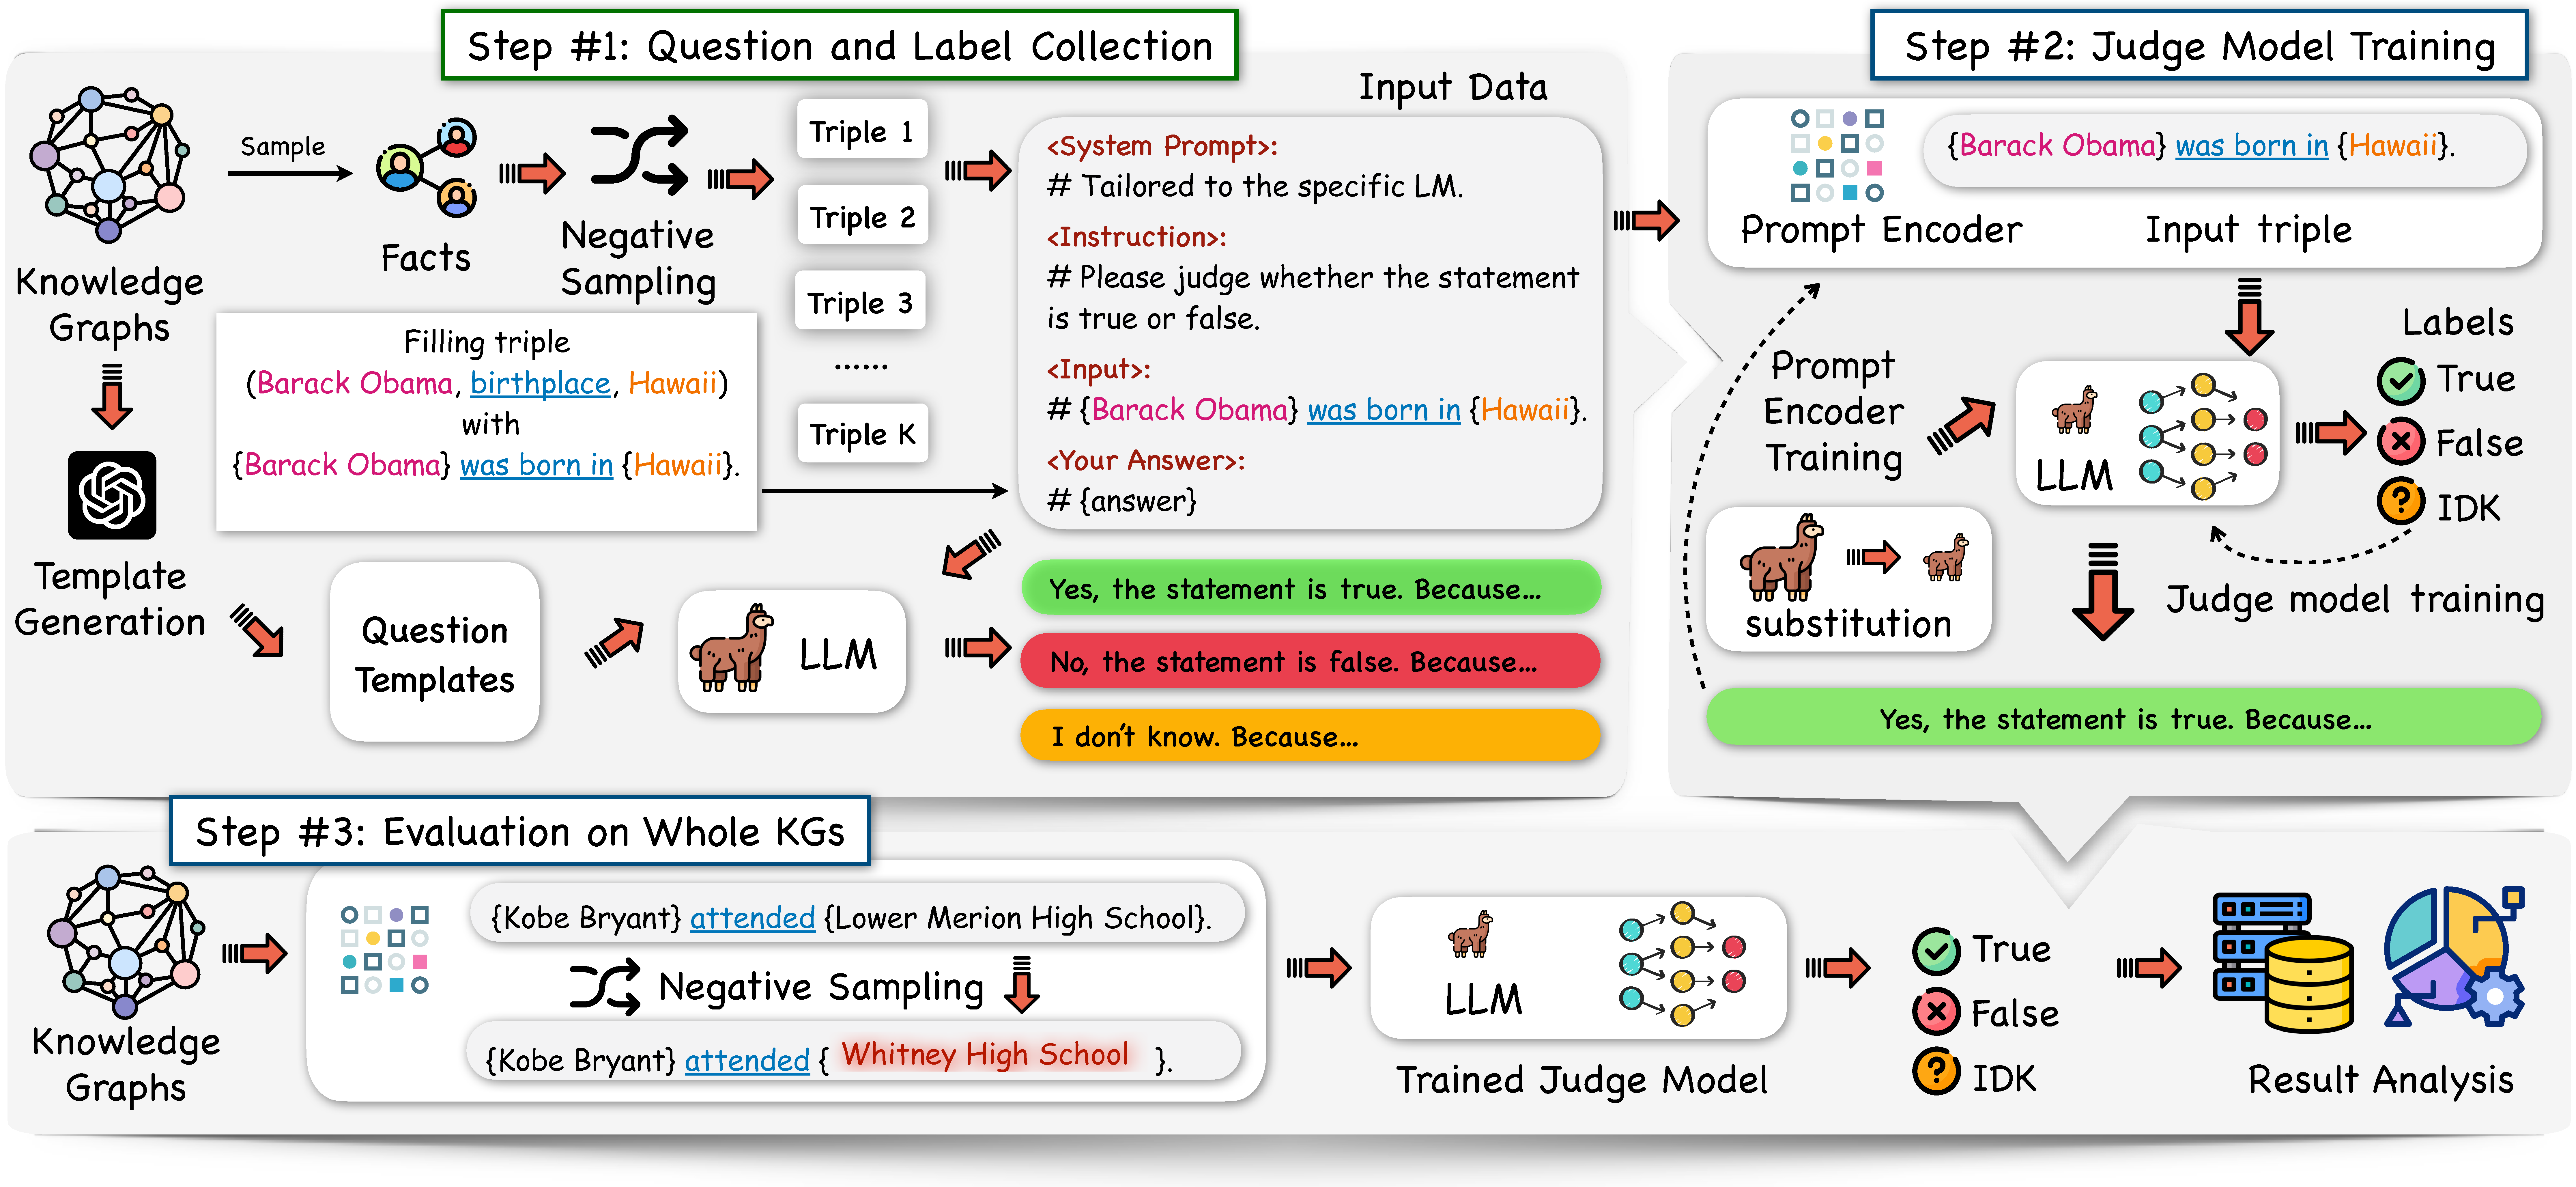
\includegraphics[width=0.65\textwidth]{
%NSFcore-2023/framework.pdf}
 %%\caption{Proposed Project}\label{project}
%\end{wrapfigure}



%We intend to propose complete, partial (either order or unordered), and various qualitative individual preference elicitation models.  An example of the first two would be having complete or only top-$k$ order of preferences over the candidates as inputs, whereas, an example of the last one  would be to bucketize candidates in different qualitative groups (recall the motivating example). For fairness, our effort would be to design group based fairness criteria designed over the protected attributes of the candidates that resemble group fairness criteria, such as, demographic parity, or statistical parity, studied in the context of classification~\cite{verma2018fairness}. To that end, we will adapt proportionate-fairness or p-fairness~\cite{pfair,chairman}  from resource allocation theory that ensures proportionate representation of every group based on a protected attribute in every position of the produced results, or its generalization~\cite{amer2009group} adapted from the social choice theory to promote affirmative action~\cite{fu2006theory} in the produced results.  
%Preference aggregation would be studied considering Kendall-Tau and Spearman's Footrule Distance functions~\cite{kemeny,diaconis1977spearman}, with the objective to minimize the sum of disagreement (Kemeny Optimization) or such, akin to existing {\em (fairness unaware) classical rank aggregation problem}~\cite{dwork2001rank,ailon2008aggregating, ailon2010aggregation}. Our goal would be to make these solutions fairness aware by investigating how to combine these two somewhat conflicting aspects in a systematic manner. For each of these proposed problem variants, we shall analyze the nature of the problem analytically and design scalable solutions with theoretical guarantees. Finally, we will perform both qualitative and quantitative study to develop actionable interventions by leveraging our proposed framework to promote fairness in two compelling applications: (i) Ranked Choice Voting (RCV)~\cite{rcv1,rcv2}, and (ii) Gender and diversity gap in the Oscars. We intend to fine-tune our proposed models based on these evaluations. 

\noindent {\bf Comparison with Existing Work.}
This contribution builds on our work recent works on fairness~\cite{islam2022satisfying, wei2022rank}, and prior works on preference aggregation~\cite{amer2009group, amer2015group, basu2015group}, studying robustness~\cite{roy2014exploiting}. We acknowledge that the existing popular group based fairness definition, such as, {\em statistical parity}~\cite{dwork2012fairness} is somewhat similar to one of our proposed fairness notion. However, the best adapted version of top-$k$ statistical parity studied in a recent paper~\cite{vldbrank} does not account for proportionate representation in every position of the top-$k$, limiting its applicability.  Studying computational challenges related to computing the margin of victory  has been a focus of recent research~\cite{stv1,stv2, stv3} in the context of electoral voting and related applications. But none of these existing works study the general version of the problem, which is, how to promote additional simple/complex constraints/criteria in the output, which is our primary focus. Other than these prior works, which are  much narrow in scope, we are unaware of any computational work that systematically studies different preference elicitation models, multiple output changing criteria, and preference aggregation combining these two.  

%Section~\ref{related} provides an in-depth comparison between our proposed work and existing work.  
%To the best of our knowledge, we are the first to investigate a generic framework that can minimally update original outcome of preference aggregation to satisfy complex constraints without any assumption on the relationship among the attributes.

%Using the aforementioned example, if $k=12$, existing work~\cite{vldbrank} only ensures p-fairness of the aggregated rank at position $12$, but not for the remaining positions (e.g., 1 to 11). {\em While p-fairness promotes stronger notion of fairness, and our proposed framework adapts to top-$k$ statistical parity, existing work does not adapt to our proposed optimization framework}.

%\smallskip \noindent {\bf Aim 1 - Fair Rank Aggregation.}
%We will begin our study in the context of ranking, which is a commonly used method to prioritize  desirable outcomes among a set of candidates and is an essential step in  many high impact applications. Here the members elicit a {\em complete preference order} over the candidates and the goal is to produce an aggregated ranked order over all candidates or produce top-$k$ results that minimize disagreements  among individual preferences. When fairness is studied, our goal would be to ensure fair representation of the candidates based on their one or more protected attributes (such as, gender, race, etc.) in the ranked order. 
%\smallskip \noindent {\bf Aim 2 - Fair Partial and Qualitative Preference Aggregation.}
%In this aim we shall consider scenarios where either qualitative preferences or partial rankings are elicited from the members. 
%We consider three such preferences: (1) top-$t$ ranking, where the input preference is a ranking of the top-$t$ items (candidates), (2) subset selection, where the input preference is an unordered subset of favorite elements, and (3) bucketing, where the input preference is a partition of the elements into three subsets: the ``yes'' set, ``ambivalent'' set, and the ``no'' set.  In our preliminary work, we consider the selection of council members or a committee of $k$ members from $n$ candidates considering the votes of $m$ judges (voters) ({\em ranked choice voting}~\cite{rank1} could be considered as a popular application of that).  The fairness criterion models affirmative action and includes a lower and upper bound on the number of elected candidates, for each value of the protected attributes(s). We intend to study the design choices of different preference elicitation models considering fairness, formalize the optimization problems and analyze them, and design principled solutions with guarantees.

%The mechanism we focus on to aggregate the top-$k$ rankings is {\em Ranked choice voting (RCV)}, and specifically RCV employing a single transferable vote (STV) system~\cite{rcvdesc}.
%We are going to follow the mechanism used in Cambridge MA to elect its city council. 

%\smallskip \noindent {\bf Aim 3 - Actionable Fair Preference Aggregation.}
%Although the proposed models and algorithms consider 
%fairness in its design, rather than an afterthought, the third aim will delve deeper into fairness considerations of compelling applications and develop actionable interventions. In particular, the third aim will provide a holistic large-scale study over two compelling applications and present actionable interventions to promote fairness. In the first application, we will study fairness in Ranked Choice Voting (RCV)\footnote{\small https://qz.com/1676718/the-pros-and-cons-of-ranked-choice-voting/} considering the data provided by the Cambridge, MA
%City Council Election 2019~\cite{RCV} to analytically answer important questions raised in recent research~\cite{rcv1,rcv2,rcv3, rcv4,rcv5}. 1. Does more choice lead to reduced racially polarized voting? 2. Does ranked choice voting enable minority representation?  Based on the analysis, {\em we will develop actionable interventions by leveraging our proposed framework to mitigate these risks}. We will perform both qualitative and quantitative analysis. For qualitative  analysis, we will recruit experienced workers from Amazon Mechanical Turk (the budget justification provided further details). A similar  study would be conducted to investigate the gender and diversity gap in the Academy of Motion Picture Arts and Sciences decisions by combining it with large scale Movielens~\cite{movielens} data and we will develop actionable recommendation to mitigate the gap. Further evaluation plan considering other datasets is described in Section~\ref{eval}.

%\section{Introduction}

Large Language Models (LLMs), despite their impressive performance across various natural language understanding tasks, exhibit significant limitations when applied to enterprise applications in the wild.
Primarily, these models may hallucinate—generating plausible-sounding but factually incorrect content—when their parametric knowledge does not align with specific enterprise data~\cite{maynez2020faithfulness,semnani2023wikichat,feng2024cmdbench}
. An LLM's parametric knowledge depends on its pre-training corpus and can also be influenced by the chosen training strategy and model architecture. This gap is especially problematic since enterprise applications frequently use private, on-premises data, which may differ substantially from the domains in LLMs' pre-training corpora.
Such domain misalignment can lead to severe inaccuracies, where the LLMs produce unreliable or misleading information.
%
In addition, enterprises often require consistency and reliability in their outputs. However, LLMs can be sensitive to prompt wording \cite{sclar2024quantifying}, producing inconsistent results even with minor phrasing changes, which undermines their reliability in high-stakes enterprise tasks.


Another key challenge for LLMs in enterprise settings is their limited capacity for complex reasoning. Many tasks in this domain require multi-step reasoning, deep contextual understanding, and coherent integration across different data sources, models, and pipelines. LLMs are not inherently designed to manage such complexities without extensive, task-specific adaptation and external grounding. These limitations hinder adopting LLMs in enterprise fields where accuracy, consistency, and reasoning depth are critical, such as healthcare, legal, HR, and data-driven decision-making applications.



%
Several approaches can help mitigate these limitations, including controlled generation, fact-checking, and post-processing. Controlled generation seeks to constrain the outputs of LLMs by guiding the model toward more reliable responses through techniques such as prompt engineering~\cite{brown2020language,wei2022chain,sahoo2024systematic}, fine-tuning~\cite{houlsby2019parameter,qin2023towards}, and reinforcement learning from human feedback~\cite{ouyang2022training}.
Fact-checking~\cite{thorne-etal-2018-fever,aly2021feverous} involves verifying generated content against highly credible sources to ensure accuracy, with any identified inaccuracies filtered out or corrected during post-processing. 
Although these techniques offer improvements, they may still struggle with domain-specific challenges and rapidly evolving knowledge.
\begin{figure}[t!] 
  %\vspace{-10pt}
  \centering
  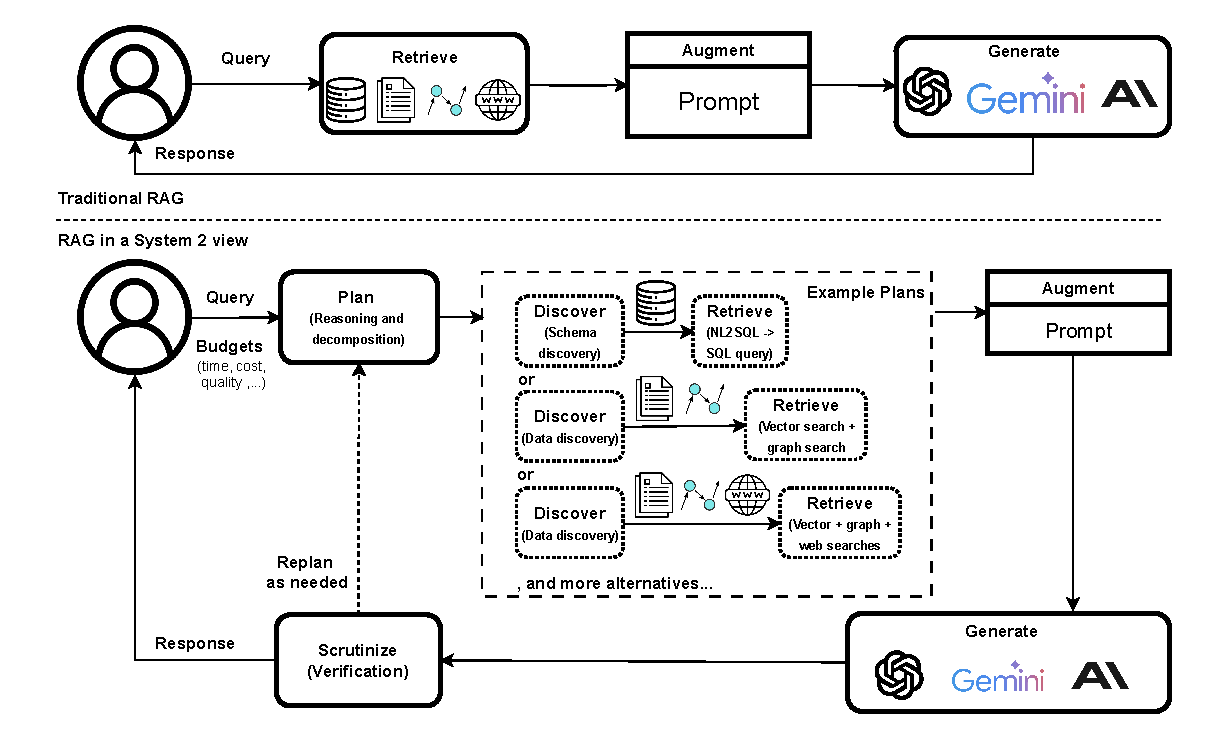
\includegraphics[width=\linewidth]{submissions/Estevam2024/figures/sys-rag2.pdf}
  \caption{Compared to the traditional RAG setup (above), where a fixed Retrieval-Augmentation-Generation workflow is executed, a System 2 approach (below) involves more deliberate reasoning and action based on critical analysis. For instance, given the same user query, the system must first plan by analyzing the task and may decide to decompose it into smaller components, such as data discovery, natural language-to-query translation, and actual query execution. During the planning phase, constraints or budgets related to factors like time, cost, or quality, along with the nature of the multimodal data sources, may influence the direction of the workflow. After the generation step, a verification process is typically required to evaluate the outcome, which may lead to revisions in subsequent iterations.}
  \label{fig:sys-rag2} 
\end{figure}
Among the various approaches, augmenting LLMs with external information sources has emerged as one of the most widely adopted solutions for enhancing accuracy and robustness. 
This strategy enables LLMs to access up-to-date, domain-specific knowledge, making them more adaptable to new fields or emerging topics. 
Techniques like retrieval-augmented generation (RAG)~\cite{lewis2020retrieval} integrate external databases or knowledge graphs to ground the model's outputs in verifiable information. 
By incorporating external data, such as multi-modal documents or enterprise-specific datasets, LLMs can produce more accurate and contextually relevant responses, thereby reducing the likelihood of hallucinations and making them more suitable for critical applications. However, simply using RAG approaches is not necessarily yet the definitive solution. Challenges remain, such as ensuring the quality and reliability of the retrieved information, handling ambiguous or conflicting data, and seamlessly integrating retrieval with generation to maintain coherent and contextually appropriate responses. Consequently, there is still considerable room for improvement in creating more robust and reliable AI systems.



As already shown in the literature, the idea of \emph{System 1} and \emph{System 2} \cite{kahneman_thinking_2012},  can be helpful to contextualize the current capabilities and limitations of LLMs \cite{bengio2019system}. In cognitive sciences, \emph{System 1} refers to fast, intuitive, and automatic thinking. This type of system can be characterized by fast thinking or quick judgments and decisions that rely on heuristics and subconscious processing. System 1 is highly efficient for everyday tasks that require intuitive, fast, unconscious, and immediate responses.
System 2, however, is associated with slow, deliberate, and analytical thinking. It is more helpful and used for complex problem-solving, critical analysis, and tasks that require conscious, sequential, algorithmic planning and reasoning. System 2 is more resource-intensive and slower but more reliable for tasks requiring careful consideration. 

In this System~1/System~2 context, we argue that even though RAG approaches have strong potential to contribute to reducing limitations of current LLMs (by playing a role more closely related to System 2), most current RAG approaches only weakly resemble System 2 thinking. The retrieval and generation steps are often designed to be fast and instantaneous, aligning with System 1 thinking, rather than slow and logical as in System 2, which presents challenges on both the data and model sides. For example, research \cite{maekawa-etal-2024-retrieval,ding2024retrieve} has shown that augmenting LLMs with retrieval without rigorously assessing necessity may adversely impact overall performance. 



Therefore, as illustrated in Figure~\ref{fig:sys-rag2}, we advocate for a shift from traditional single-model architectures to compound AI systems within a System 2 framework to enhance RAG, particularly in complex enterprise applications. Compound systems enable a collaborative approach to problem-solving by distributing specialized tasks across distinct agents, each optimized for specific functions, improving both retrieval and generation performance in challenging real-world settings.

On the retrieval side, enterprise applications often involve complex, multi-step, and sometimes ambiguous tasks that require deeper reasoning and structured workflows. A compound system can enhance this by assigning specialized agents to handle diverse aspects of data, such as heterogeneous formats (e.g., text, tables, graphs, parametric information) and noisy or incomplete data sources. This allows for agents skilled in reconciliation and semantic querying to refine the retrieval process through iterative, logic-driven interaction, improving both precision and relevance of context.

On the generation side, challenges like hallucination, fact verification, and adherence to context remain key obstacles. In a compound system setup, individual agents can be tasked with verifying facts, maintaining context alignment, and evaluating outputs for accuracy before finalizing responses. This division of labor can be exploited towards reducing hallucinations and enhancing reliability by enabling dynamic inter-agent evaluation, where each agent iteratively cross-checks and validates the others' outputs \cite{zhang2021survey,carlson2010toward}. For example, in domain-specific conversational AI, particularly in regulated industries, compound AI systems offer a pathway to safer, more reliable, and robust deployments by integrating domain expertise, context sensitivity, and rigorous validation at each step. 


The paper is organized as follows. First, in \cref{sec:background}, we provide a brief overview of traditional RAG models and highlight their limitations, especially in real-world, domain-specific applications. We then motivate more concretely the need for a System 2 RAG approach, in section 3. In \cref{sec:sys2}, several approaches to enhance RAG adaptability to System 2 thinking are discussed. Finally, we present our vision for future research in \cref{sec:future}, exploring the potential of compound AI systems as System 2 solutions to RAG.


%\input{IEEE-data-engineering-IC1/preliminary}
\vspace{-0.2in}
\section{Formalism}\label{preliminary}
\vspace{-0.1in}
%The proposed work aims at developing an optimization guided computational framework that modifies an output obtained from a preference aggregation method applied on a preference elicitation model to produce a modified output that satisfies given criteria. The proposed work aims at developing this framework for a suite of preference elicitation models and preference aggregation methods.
%that satisfies with criteria that guides the need to change the original output minimally while producing a complete or top-$k$ (ordered or unordered) result aggregating individual preferences.

There are $4$ types of inputs that our proposed framework takes: (a)~a set $N$ of $n$ items, where each item has a set $\mathcal{A}$ of discrete attributes.  Each attribute $a\in \mathcal{A}$ has $\ell_a$ different values. (b)~a set of $m$ users, where the $i$-th user $u(i)$ provides her preference as $\sigma_i$. The users' preferences could be rank based, partial or full order, or non rank based. (c)~a distance function $\mathcal{F}$ (defined formally below) that measure the ``distance'' between a set of $m$ input preferences  $\sigma_1, \sigma_2,\ldots, \sigma_m$ and an output $\sigma$ with the required output form. The exact distance function depends on the underlying preference elicitation model and the required output form which may be either a complete ranking of the items or a subset of $k$ items, either ranked or not. (d)~a set $\mathcal{C}$ of output criteria/constraints. Some variants of our problem also include as input a budgetary constraint $B$.

%The proposed work aims at developing an optimization guided computational framework that suitably combines a suite of preference elicitation models with criteria that guides the need to change the original output minimally while producing a complete or top-$k$ (ordered or unordered) result aggregating individual preferences. %Next, we present some definitions that will be used throughout the proposal.  

\begin{definition}\label{def4}
\vspace{-0.1in}
{\bf Distance function $\mathcal{F}$.} Given $m$ input preferences  $\sigma_1, \sigma_2,\ldots, \sigma_m$ and an output $\sigma$ with the required output form, the function $\mathcal{F}(\sigma, \sigma_1, \sigma_2,\ldots, \sigma_m)$ is the distance of $\sigma$ from the input preferences  $\sigma_1, \sigma_2,\ldots, \sigma_m$.
In some cases the function $\mathcal{F}(\cdot)$ is an aggregation of a distance function between a single input preference and the output. Examples for such an aggregation are the sum of the pairwise distances and the maximum distance to any of the input preferences. In other cases $\mathcal{F}(\cdot)$ measures the minimum modification of the input preferences that would result in the preference aggregation method outputting the output $\sigma$. 
%$\mathcal{F}(\sigma, [\sigma_1, \sigma_2,\ldots, \sigma_m])$
\end{definition}

\vspace{-0.1in}
\begin{definition}\label{def1}
\vspace{-0.1in}
{\bf Output criteria/constraints.}  For an attribute $a\in \mathcal{A}$,  let $c(p_a)$ denote the cardinality constraints of items with value $p_a$ ($p_a$ is one of the $\ell_a$ possible values of attribute $a$). Given to the framework is a set $C$ of such cardinality constraints for each attribute value $p_a$, for every $a \in A$, $A \subset \mathcal{A}$. There are two explicit cases that we consider.
\begin{itemize}
    \item {\bf The output $\sigma$ is ordered and consists of $k\le n$ items.} 
    In this case the cardinality constraints are defined for every $\kappa \in [1..k]$ items, and for every  such $\kappa \in [1..k]$, the $\kappa$ top ranked items of output $\sigma$ have to satisfy these cardinality constraints.  
    %the $k$ top ranked items satisfy all cardinality constraints defined over $v$, i.e., it satisfies $c(p^v_{a_1}) \text{ AND } c(p^v_{a_2}) \text{ AND } \ldots \text{ AND } c(p^v_{a_A})$.  
     \item {\bf The output $\sigma$ is an unordered set of $k$ items.} In this case the cardinality constraints are defined for $k$ items and the items in the output set $\sigma$ have to satisfy these cardinality constraints. 
     \\ %$c(p_{a_1}) \text{ AND } c(p_{a_2}) \text{ AND }  \ldots \text{ AND } c(p_{a_A})$.  
\end{itemize}  
\end{definition}
\vspace{-0.1in}
\begin{definition}\label{def3}
\vspace{-0.1in}
{\bf A budgetary constraint.} A budgetary constraint $B$ is an upper bound on the distance of the output from the input preferences. 
%For a given distance function $\mathcal{F}(\cdot)$, 
The budgetary constraint implies that $\mathcal{F}(\sigma,\sigma_1,\sigma_2,\ldots,\sigma_m)\leq B$.  
\end{definition}

\vspace{-0.1in}
\begin{definition}\label{def2}
{\bf Preference Aggregation Considering Constraints.} 
We intend to study different types of problem definitions that require different algorithmic treatments.
Given either complete or partial preferences $\sigma_1,\sigma_2,\ldots,\sigma_m$ over the items in $N$, a preference aggregation method, a distance function $\mathcal{F}(\cdot)$, and a set of output criteria $\mathcal{C}$.
\vspace{-0.1in}
\begin{itemize}
    \item {\bf (Constrained optimization).} Produce an output $\sigma$ with the required form that minimizes $\mathcal{F}(\sigma,\sigma_1,\sigma_2,\ldots,\sigma_m)$ and satisfies $\mathcal{C}$.
    \vspace{-0.1in}
    \item {\bf (Optimization under budgetary constraints).} Produce an output $\sigma$ with the required form that optimizes $\mathcal{C}$,  while satisfying $\mathcal{F}(\sigma,\sigma_1,\sigma_2,\ldots,\sigma_m) \leq B$. (The objective function for optimizing $\mathcal{C}$ varies.)
    \vspace{-0.1in}
    \item {\bf (Bi-criteria optimization).} Given parameters $\alpha$ and $\beta$ produce an output $\sigma$ with the required form that satisfies both $\mathcal{F}(\sigma,\sigma_1,\ldots,\sigma_m) \le \alpha$ and $\mathcal{G}(\mathcal{C}) \le \beta$, where $\mathcal{G}$ is the objective function for optimizing $\mathcal{C}$.
\end{itemize}
\end{definition}
%The individual research aims will describe the various forms of preference elicitation from users and the details of the preference aggregation methods. We first delineate the need to change original output and the challenges that arise from there.
\vspace{-0.1in}
\subsection{Specifying Output Criteria}
We discuss orthogonal reasons where the original outputs coming out of the preference aggregation methods need to be ``massaged'' further. What unifies them is that these criteria are defined over one or more attributes of the items. Depending on how many attributes are involved in the definition and their relationship thereof gives rise to additional challenges.


%\vspace{-0.1in}
%\subsection{Important Concepts and Definitions}\label{pre}
%\vspace{-0.1in}
%\noindent \textbf{Database.} contains $n$ items or candidates. These two terms will be used interchangeably. The set of items will be denoted $V$, individual items will be denoted by $u$ and $v$. \\
%\noindent {\em \bf Individual preference Elicitation:} We consider the following individual preference elicitation models. \\
%\noindent (1) Complete preference: Each of the $4$ members (Judges) may provide a {\em complete order of preference} over the $12$ candidates (Refer to Table~\ref{tab:example_original_rank}). \\
%\noindent (2) Partial preference: 
%(2.1) Ordered. Member 1 (as well as other members) may provide a partial order over the first $5$ candidates and does not specify anything for the rest.\\
%(2.2) Unordered. Member 1 (as well as other members) may also specify that she likes the first $5$ candidates without specifying any order among them.\\
%\noindent (3) Qualitative Preference: Contrarily, Member 1 (as well as other members) may provide {\em qualitative preferences}: Molly and Amy are preferred, Abigail, Kim, Lee are acceptable, the remaining ones must not be considered. These are considered to be the inputs to the framework. Please note that 2.2 is a simplified variant of this last preference elicitation model.

%\noindent \textbf{Multiple Preferences.} The input consists $m$ different preference elicitation (based on the individual models described above). Using the motivating example, $m=4$.

\subsubsection{Fair Preference Aggregation}
We will study fairness in the context of group based protected attributes of the candidates. Output criteria/constraints for fairness (refer to Definition~\ref{def1}) are expressed over one or more {\em protected attributes}. Their protected attributes could be expressed over gender, ethnicity, race, or the state the candidates are living in. 

Formally speaking, each item/candidate $v\in N$ has one or more  {\em protected attributes}. When $\ell_a=2$, it is a binary protected attribute; when $\ell_a \geq 2$ it is a multi-valued protected attribute. As an example, race is (usually) a multi-valued protected attribute, and gender is sometimes a binary protected attribute.

%\begin{itemize}
%\item  {\bf p-fairness.} 
\smallskip \noindent \textbf{p-fairness.}
p-fairness has been studied in the context of resource allocation satisfying temporal fairness or proportionate progress~\cite{chairman, pfair}. It was introduced in the classical  {\em Chairman Assignment Problem}~\cite{baayen1964existence, chairman} that studies how to select a chairman of an union every year from a set of  $n$ states such that  that at any time the accumulated number of chairmen from each state is proportional to its weight. 

In the context of ranking, suppose that each of the $n$ ranked items has a {\em protected attribute} $a(\cdot)$ that can take any of $\ell_a$ different values. For $p_a\in [1..\ell_a]$, let $c'(p_a)$ denote the fraction of items with protected attribute value $p_a$, that is, $c'(p_a) = \frac 1n \sum_{i=1}^n \bbone_{a(i)=p_a}$. The goal is to ensure that $c'(p_a)$ fraction (rounded either up or down) of every top $\kappa$ items have protected attribute value $p_a$.
\iffalse
\vspace{-0.1in}
\item {\bf Generalization of p-fairness to promote affirmative action.} Instead of requiring $c'(p_a)$ fraction of every top $\kappa$ items to have protected attribute value $p_a$, we may want that certain values of the protected attribute get higher representation among the elements at the top, more than their overall proportion. Let $P$ be a non-negative doubly stochastic $n \cdot \ell_a$ matrix. The goal is to ensure that $P(\kappa,p_a)$ fractions (rounded either up or down) of the top $\kappa$ items to have value $p_a$, for every $\kappa \in [1..n]$ and $p_a\in [1..\ell_a]$ (if it is feasible).
It is not difficult to note that such a generalized notion can capture affirmative action.
%\end{itemize}
\fi


\subsubsection{Robust Preference Aggregation}
Output criteria/constraints for robustness on the other hand investigates the flip questions: Given either complete or partial preferences $\sigma_1,\sigma_2,\ldots,\sigma_m$ over $n$ items, let $\sigma$ be the output obtained by the preference aggregation method. Given a budget $B$, how to  make $B$ or less changes in the original preferences, such that the outcome is different from $\sigma$? This question is  related to finding the {\em margin} in electoral systems and quantifies how manipulable the underlying aggregation method is. We study this problem under different manipulation models -- addition only, deletion only, or substitution (addition + deletion).

\iffalse
\subsection{Challenges in Handling  Complex Output  Criteria}
In general, the output requirements/constraints are defined over a set $R$ of attributes. When $|R|=1$, as an example, the output requirement is defined on a single attribute (such as race). In a recent work, we demonstrated that for an aggregation method that models plurality voting, the problem of preference aggregation while satisfying output criteria defined by a single attribute is computationally easy. 
However, the nature of the problem changes when two or more attributes are involved in the output criteria. In Section~\ref{aim1} we discuss this more complicated case and refer to our recent work in which we showed evidence that in some cases it is computationally difficult even to find any output with the required form. 
\fi
%When there are two or more different attributes involved in outlining output criteria/constraints (such as certain representation from race and certain representation from gender), the PIs have proved in a recent work~\cite{islam2022satisfying} that the decision version of the preference aggregation problem under output constraint becomes (weakly) NP-hard by reducing the well known NP-hard Partition problem to our problem~\cite{garey1979computers}. We note that the existing practice of converting multiple attributes to a single multi-valued protected attribute by computing joint distribution over the attributes assumes independence among the attributes. When Independence among the attributes does not hold, this simplification leads to a heuristic process.  The PIs have also demonstrated that for three (or more) attributes (e.g., constraints defined over race, and gender, and ethnicity), even the question whether there exists a set of top-$k$ that satisfies the complex constraint is strongly NP-Hard where the reduction is fro 3 Dimensional Matching. On the positive side for the case of two  attributes, the PIs have designed an efficient algorithm a preference aggregation algorithm while satisfying fairness constraints defined over $2$ attributes and has designed a 2 approximation factor and runs in $O(n^2\ell \log m)$ time, by casting this problem as a min cost flow problem, where $\ell$ is the total number of possible attribute values. We intend to study these aspects in the proposal - as it turns out to be an intellectually demanding and independent  facet of the computational problem, irrespective of the specific reasons to change the output.


%\input{IEEE-data-engineering-IC1/aim1}
\vspace{-0.2in}
\section{Single Round Rank based Preference Aggregation}\label{aim1}
\vspace{-0.1in}
We outline two separate lines of algorithmic problems: (1) incorporating output criteria (e.g., p-fairness) in single round rank-based preference aggregation methods, and (2) satisfying complex constraints in single round rank-based preference aggregation methods.
\vspace{-0.1in}
\subsection{Incorporating output criteria in rank aggregation} 
\vspace{-0.1in}
The input to the classical {\em rank aggregation} problem consists of $m$ complete order of preferences over the $n$ items/candidates. Traditionally, producing the final ranking involves aggregating potentially conflicting preferences from multiple individuals, and is known as the rank aggregation problem~\cite{dwork2001rank,van2007deterministic, ailon2008aggregating}. Our goal is to  minimally change the aggregated output to enable fairness.
%p-fairness has been studied in the theory community to enable resource allocation satisfying temporal fairness or proportionate progress.
We will study p-fairness~\cite{chairman, pfair} that ensures proportionate representation of every group based on a protected attribute in every position of the aggregated ranked order.  The classical problem in this context is known as the {\em Chairman Assignment Problem}~\cite{baayen1964existence, chairman} which studies how to select a chairman of a union every year from a set of  $r$ states such that  that at any time the accumulated number of chairmen from each state is proportional to its weight. p-fairness generalizes other notions of fairness~\cite{islam2023equitable} that were considered in prior work, including the existing popular group based fairness definition {\em statistical parity}~\cite{dwork2012fairness}. 
%We start with some definitions and then describe both our preliminary research and the open problems we plan to investigate further.
\vspace{-0.1in}
\subsubsection{Research Directions}
\vspace{-0.1in}
%\noindent \textbf{Rank and Multiple Ranking.}  
Consider rankings of the items in a set $V$. Each such ranking can be viewed as a permutation. We will use the terms ranking and permutation interchangeably. 

\noindent \textbf{Kendall-Tau and Kemeny distances.}
	Given two rankings $\sigma,\eta: V \rightarrow [1..n]$, the
	Kendall-Tau distance between the two rankings is the sum of pairwise disagreements between $\sigma$ and $\eta$ (bubble-sort distance)
	\[
	\cK (\sigma,\eta) = \sum_{\{u,v\}\subseteq V} \bbone_{(\sigma(v)-\sigma(u))(\eta(v)-\eta(u))<0}.
	\]
	
	For a set of rankings
	$\{\eta_1,\eta_2,\ldots,\eta_m\}$ the {\em Kemeny distance} of the ranking
	$\sigma$ to this set as
	\[
	\kappa(\sigma,\eta_1,\eta_2,\ldots,\eta_m)= \sum_{i=1}^m \cK (\sigma,\eta_i).
	\]

 \noindent \textbf{Spearman's footrule distance.}
    Given two rankings $\sigma,\eta: V \rightarrow [1..n]$, the 	Spearman's footrule distance between the two rankings is the sum of the absolute values
  ($\ell_1$ distance) of the differences between rankings $\sigma$ and $\eta$.
	\[
	\cS (\sigma,\eta) = \sum_{u\in V} |(\sigma(u)-\eta(u)|
	\]
 
	For a set of rankings
	$\{\eta_1,\eta_2,\ldots,\eta_m\}$ the {\em Spearman's footrule distance} of the ranking
	$\sigma$ to this set is the sum of the pairwise distances.

    \noindent \textbf{Rank aggregation.} The aggregated ranking of a set of $m$ rankings $\{\rho_1,\rho_2,\ldots,\rho_m\}$ for a given distance function is a ranking that minimizes  the distance to this set.
    
    \noindent \textbf{p-fairness for a ranking.}
    For a permutation $\sigma, k\in [1..n], p\in [1..\ell]$, let $P(\sigma,k,p)$ denote
    the number of elements with protected attribute value $p$ among the $k$ top ranked elements
    in $\sigma$. A ranking $\sigma$ is {\em proportionate fair} or {\em p-fair} if
    \[
    \forall k\in [1..n]\, \forall p\in [1..\ell]:\  P(\sigma,k,p)\in \{\floor{f(p)\cdot k},\ceil{f(p)\cdot k}\}.
    \]

 
%We note that the best adapted version of top-$k$ statistical parity studied in a recent paper~\cite{vldbrank} does not account for proportionate representation in every position in the top-$k$ positions, but just to a small number of positions, thus limiting its applicability.
%As a matter of fact it can be shown that the algorithm Fair-ILP presented in~\cite{vldbrank} for the special case of a binary protected attribute in which the frequency of both values is the same may produce a very skewed output. This is because the algorithm Fair-ILP just considers the {\em total number of times} items with one value of protected attribute are ranked above items with the other value. p-fairness is  stronger because it ensures statistical parity for every position in the ranked order and considers, for every $k$, the number of times items in the top-$k$ with one value of protected attribute are ranked above items with the other value. This makes this notion of fairness significantly harder to implement and the existing solutions do not trivially adapt.


We formalized two optimization problems, individual p-fairness or {\bf IPF} and the rank aggregation problem subject to proportionate fairness ({\bf RAPF})  considering binary ($\ell=2$) and multi-valued ($\ell > 2$) protected attributes. These problems and associated algorithmic results could be found in~\cite{wei2022rank}.


\vspace{-0.1in}
\subsubsection{Open Problems}
\vspace{-0.1in}
We plan to investigate the following open problems.

\smallskip \noindent{\bf p-fairest aggregate ranking (PFAR).} 
The PFAR problem is defined as follows. Given a set of $m$ rankings %$\{\rho_1,\rho_2,\ldots,\rho_m\}$ 
choose the ``p-fairest'' ranking among all rankings that minimize the Kemeny distance to this set. 
We need to define ``p-fairest'' ranking or a distance measure to a p-fair ranking.
We propose the following distance measure (using the notations defined above).
For an integer $d \ge 0$, a ranking $\sigma$ is at distance $d$ from a {\em p-fair} ranking if
\[
\forall k\in [1..n]\, \forall p\in [1..\ell]:\  P(\sigma,k,p)\in \{\floor{f(p)\cdot k}-d,\ceil{f(p)\cdot k}+d\}.
\]

\iffalse
Another way to view the distance to a p-fair ranking is by considering the classical {\em p-processor cup game} defined by Liu~\cite{liu1969} that considered the notion of p-fairness in multi processor scheduling. The p-processor cup game (adapted to our case) is a multi-round game with two players, an {\em emptier} and a {\em filler}, that takes place on $\ell$ cups, each filled initially with a fixed amount of water, called {\em buffer}. At the beginning of each round,
the filler adds a total of 1 gallon of water to the cups. The distribution of this 1 gallon to the cups is determined by the filler.
The emptier then selects a single cup (that must have at least 1 gallon of water)
and removes 1 gallon from this cup. The emptier’s goal is to minimize the size of the buffer and the {\em backlog} which is the amount of water (on top of the initial amount) in the fullest cup.

It is easy to see the analogy to p-fairness. Consider a p-fair ranking of $n$ elements each with a protected attribute with $\ell$ possible values. Each cup represents a possible value of the protected attribute. The corresponding game has $n$ rounds. In each round $k\in [1..n]$ the filler
adds $f(p)$ gallons of water to cup $p$, for $p\in [1..\ell]$, and the emptier removes 1 gallon of water from the cup corresponding to the value of the protected attribute of the element ranked $k$.
The existence of a p-fair ranking implies that the emptier can always guarantee that the size of the buffer and the backlog is no more than 1 gallon.
For a ranking that is at distance $d$ from a p-fair ranking, the emptier can guarantee that the size of the buffer and the backlog is no more than $1+d$ gallons.
\fi

We observe that PFAR is also NP-Hard as directly follows from the fact that unconstrained rank aggregation is NP-hard when 
$m\ge 4$~\cite{ailon2008aggregating}. For some fixed $\alpha > 1$, We would like to find an algorithm that finds the p-fairest ranking among all rankings whose Kemeny distance from the set of input rankings is at most $\alpha$ times the minimum such distance. 
%Reasonable values of $\alpha$ to consider are 
%$\frac 85$ and $\frac 43$ since there are efficient $\frac 85$ and $\frac 43$ approximation algorithm for the rank aggregation problem~\cite{ailon2008aggregating}.

\smallskip \noindent {\bf Bi-criteria p-fair rank aggregation (BPFRA).} 
The most general problem that we plan to consider in this context is the bi-criteria optimization problem, that is, for a given pair $(\alpha>1 ,\beta>1)$ and a set of $m$ rankings %$\{\rho_1,\rho_2,\ldots,\rho_m\}$
find a ranking whose Kemeny distance to the set of rankings is at most $\alpha$ times the Kemeny distance of the aggregated rank from the set and its distance from a p-fair ranking is at most $\beta$, if such a ranking exists.

\smallskip \noindent{\bf p-fair rank aggregation with affirmative action.} 
We plan to consider a variant of p-fair rank aggregation that involves ``affirmative action''. This will be modeled by varying the proportion of the values of the protected attribute in the p-fair aggregated rank. For example, consider a binary protected attribute with values A and B each needs to appear the same number of times. Suppose that our goal is to promote the items with attribute value A. In this case we can vary the proportion of A making it higher in the top ranked elements and lower in the lower ranked elements so that overall items with attribute value A will appear the same number of times as items with attribute value B.

\smallskip \noindent{\bf The complexity of individual p-fair ranking (IPF).}  We plan to further investigate the IPF problem for multi valued protected attributes as it is open whether it can be solved accurately in polynomial time. We conjecture that this problem is NP-Hard. %and plan to look for a suitable reduction to prove this conjecture. 
We also plan to look for improved approximation algorithms for this problem.
%We note that the algorithm DetConstSort given in~\cite{kddrank} does not produce closest ranking to a given input ranking.

\smallskip \noindent {\bf Better approximation of rank aggregation subject to p-fairness (RAPF).}
We plan to develop more sophisticated RAPF algorithms with better approximation ratios,  %One approach for designing such algorithms is to apply the pivoting technique presented in~\cite{ailon2008aggregating} for rank aggregation. We also plan 
and to improve the computational aspects of the RAPF problem. This problem can be formulated as an Integer Programming (IP) problem. %and thus the RAPF problem of reasonable size can be solved in practice using an IP solver like Gurobi or CPLEX.
We plan to consider various IP formulations as well as various rounding techniques to accelerate the computation.

\smallskip \noindent{\bf Robust rank aggregation.} It is known that rank aggregation under Kemeny distance is NP-hard. We will explore other aggregation methods, such as Spearman's footrule and Borda, and study how manipulable these rank aggregation methods are -- that is, if only $x\%$ of the preferences are allowed to be changed, how easy it is to change the outcome.
\vspace{-0.1in}
\subsection{Complex Constraints} 
\vspace{-0.1in}
Our goal is to optimize preference substitution to satisfy complex top-$k$ fairness constraints, where the fairness requirement is defined over a set $R$ of protected attributes. One of the objectives we will consider is {\em minimizing the number of single ballot (ranking) substitutions that guarantee fairness in the top-$k$ results.} 
%In voting theory~\cite{cary2011estimating}, the concept of margin of victory (MOV) is designed to measure electoral competitiveness of the candidates. 
In a preliminary work we defined the problem of finding the smallest number of single ballot substitutions to promote a set of $k$ candidates that satisfy fairness requirements defined over a set $R$ of protected attributes to the top-$k$. 
\vspace{-0.1in}
\subsubsection{Research Directions}
\vspace{-0.1in}
We assume that there are $\ell$ protected attributes , denoted $A_1,\dots, A_\ell$. For $i\in [1..\ell]$, attribute $A_i$ has $\ell_i$ possible values, denoted $A[i,j]$, for $j\in [1..\ell_i]$. Each candidate is associated with a specific value from each attribute.
In addition, we are given target quantities $a[i,j]$, for $i\in [1..\ell]$, and  $j\in [1..\ell_i]$, with property that all row marginals sum to $k$. Namely, for every $i\in [1..\ell]$, $\sum_{j=1}^{\ell_i} a[i,j] = k$. A fair outcome should satisfy the fairness  condition that for $i\in [1..\ell]$, and  $j\in [1..\ell_i]$, exactly $a[i,j]$ candidates whose $A_i$ attribute value is $A[i,j]$ are elected. 

\noindent We note that one way to approach this problem is by converting the multiple protected attributes to a single multi-valued protected attribute by computing joint distribution over the attributes assuming their independence. For example, instead of considering two binary valued attributes $A_1$ and $A_2$ we consider a single attribute with 4 possible values and the requirement that the value $i*j$ should appear $a[1,i]\cdot a[2,j]/k$ times, for $i,j\in \{1,2\}$. The shortcomings of this approach are two-fold: First, this approach may yield that the problem is infeasible while there is still a solution without assuming independence. A solution that assumes independence may be inferior (require more substitutions) than a solution that does not assume independence.

\noindent In~\cite{islam2022satisfying}, we showed that the problem of finding the smallest number of single ballot substitutions (original preference) to promote a set of $k$ candidates that satisfy proportionate representation over a single protected attribute is computationally easy for any domain size of the protected attribute. On the other hand the same problem becomes computationally hard if we increase the number of protected attributes. When there are two different protected attributes involved in outlining the fairness requirement, we proved that the decision version of that problem is (weakly) NP-hard, %by reducing the well known NP-hard Partition problem to our problem~\cite{garey1979computers}. 
For three (or more) protected attribute, even the question whether there exists a set of top-$k$ that satisfies the complex fairness constraint is strongly NP-Hard by a reduction from 3 Dimensional Matching. On the positive side for the case of two protected attributes we designed an efficient algorithm that obtains a 2 approximation factor and runs in $O(n^2\ell \log m)$ time, 
%by casting this problem as a min cost flow problem, 
where $\ell$ is the number of possible attribute values. We also designed an exact algorithm with running time $n^c$, where $c$ is the size of the Cartesian product of all the attribute domains.

\vspace{-0.1in}
\subsubsection{Open Problems}
\vspace{-0.1in}
There propose two possible ways to extend these problems.

\smallskip \noindent {\bf Improved approximation ratio in the case of 2 protected attributes.} 
Since  the problem of minimizing the number of single ballot substitutions in the case of 2 attributes is currently proven to be weakly NP-Hard, it may admit a PTAS (Polynomial Time Approximation Scheme). We plan to investigate the existence of a better approximation algorithm. Alternatively, we will try to improve the hardness result and show that this problem is strongly NP-Hard or Max-SNP Complete. 

\smallskip \noindent {\bf Relaxed solutions in the case of 3 or more protected attributes.} 
Clearly, the hardness result of even checking the existence of a solution in case of 3 or more attributes precludes the existence of any approximation algorithm for this case. We plan to design an algorithm that will generate a relaxed set of items/candidates. The relaxation may be in two dimensions: (i) the generated set will be a top-$k$ set of candidates but the fairness requirements will not be fully satisfied for all protected attributes. (ii) the generated set will have size larger than $k$ but it will satisfy the (lower bounds of the) fairness constraints for top $k$. Clearly, the larger the generated set is the easier the problem. We will find the smallest such extended set that guarantees the fairness  constraints imposed by all protected attributes.


%\input{IEEE-data-engineering-IC1/Aim2}
\vspace{-0.1in}
\section{Multi Round Rank based Preference Aggregation}\label{aim2}
\vspace{-0.1in}
We study algorithmic challenges to satisfy  output constraints in multi-round rank based preference aggregation methods, popularly known as ranked choice voting or (RCV)~\cite{irv1}. 
\vspace{-0.1in}
\subsection{Research Directions}
\vspace{-0.1in}
We start by describing the STV (single transferable vote) method~\cite{stv-irv, stv1} that generalizes the IRV method, and selects a set of $k$ items/candidates as the winners. STV is gaining popularity as an electoral system. It is used to elect candidates to the Australian Senate, in all elections in Malta, in most elections in the Republic of Ireland, and in Cambridge, MA. There are also plans to use STV in other USA localities. As mentioned in Section~\ref{preliminary} this method of preference aggregation is also applicable in other settings.

The input to an STV preference aggregation method consists of $m$ either complete or partial rankings of the items/candidates. Suppose that the total number of items/candidates is $n$ out of which $k$ items need to be elected. The preference aggregation process requires a predefined {\em quota}. In most cases this quota is Droop quota~\cite{droop} defined as $\floor{\frac{n}{k+1}}+1$. The aggregation is done in rounds. In each round every item/candidate is associated a {\em tally}. Initially, the tally of every item is the number of rankings in which it is ranked highest. A round starts by considering the items whose tally is at least the quota. These items are elected in non-increasing order of their tally, as long as $k$ items/candidates have not been elected (which always holds for Droop quota). When an item is elected their ``surplus'' (the number by which their tally exceeds the quota) is distributed to the next preferred item in their ranking (that has not been eliminated yet). The exact way this ``surplus'' is allocated varies. In a most cases, this allocation is done either fractionally or by a random selection of the surplus rankings out of all the  rankings in which the elected item is top ranked. This is repeated as long as there are items whose tally is at least the quota (and $k$ items/candidates have not been elected). 
Then, if less than $k$ items/candidates are elected, the item/candidate with the smallest tally is eliminated from all the rankings, and the tallies are updated based on the new rankings. If the number of items/candidates remaining (not elected and not yet eliminated) equals the
number of items/candidates left to be elected, these candidates are elected and the STV process terminates, otherwise the process repeats.

There is evidence that IRV and thus also STV preference aggregation methods are computationally hard to manipulate. It is NP-Hard to decide whether an IRV method can be manipulated even by adding one complete ranking~\cite{stv2}. On the positive side, \cite{blom2016,blom2019,magrino2011} suggested branch and bound algorithms that use Integer Programming to compute the Margin of Victory (MOV) in IRV. 

\iffalse
In our preliminary work, 
we considered the selection of $k$ council members out of $n$ {\em candidates} by $m$ voters or {\em members} with no ranking among the $k$ selected candidates. The fairness criterion %for this scenario is quite straightforward: 
is to maintain the proportion of each value of the protected attributes(s) within the selected candidates as in the whole set of candidates, or its generalization that models affirmative action and includes a lower and upper bound on the number of elected candidates, for each value of the protected attributes(s). %Since sometimes affirmative action is required, we consider a generalization where for each value of the protected attributes(s) we are given a lower and upper bound on the number of candidates with this value who have to be elected to the committee.
The challenge is how to produce a fair (or close to fair) solution that accurately reflects the opinions of the voters.

One obvious way is to elicit preference from the members is to ask each member or voter to vote for (up to) a fixed number $t \in [1..k]$ candidates and choose the $k$ candidates who received the most votes, and satisfy the fairness constraints. A clear shortcoming of this simplistic approach is that some of the elected candidates may receive very little support by the voters. For example, in case each voter casts a vote for a single candidate and one of the candidates is endorsed by, say, $90\%$ of the voters, then the rest of the elected candidates would each be elected by less than $10\%$ of the voters. 

Another option is to ask the voters to rank the candidates and then use p-fair rank aggregation as discussed earlier to identify the top $k$ candidates. This option is also not desirable. First, it requires the voters to rank all candidates. Second, this method has some inherent shortcomings as per the celebrated Arrow's impossibility theorem~\cite{arrow,fishburn1970arrow}. These shortcomings are apparent in the specific rank aggregation method used earlier, as this method satisfies the {\em extended Condorcet criterion}, and thus may give total power to a slim majority, ignoring the opinion of a sizable minority. For example, consider the case of $100$ voters and $26$ candidates among whom 13 candidates need to be elected.
Denote the candidates by the letters $A,\ldots,Z$. Suppose that 51 of the voters rank the candidates in order from $A$ to $Z$ while 49 of the voters rank the candidates in reverse order from $Z$ to $A$. The aggregated rank will be $A,\ldots,Z$, implying that the 13 elected candidates will be $A,\ldots, M$, and none of the candidates preferred by 49 of the voters will be elected.

An alternative option that we explore and is regaining popularity recently is the {\em ranked choice voting (RCV)}~\cite{rank1}, and specifically RCV employing a {\em single transferable vote (STV)} system. An STV-RCV means an electoral system in which voters rank up to a fixed $t \in [1..k]$ candidates and ballots transfer to next‐ranked picks until all seats are filled. Broadly, such systems can facilitate majority winners in single‐seat elections, and majority rule with minority representation in multi‐seat elections. There are numerous mechanisms to determine the winners in an STV-RCV. We follow the mechanism used in Cambridge MA to elect its city council as described below (source~\cite{rcvdesc}).

Once ranked ballots have been collected, winners are determined in rounds that are repeated as long as there are still seats that need to be filled.
Each round is called a {\em count}. 
A {\em quota} is set to $q=\floor{n/(k+1)}+1$. %$q=\floor{\frac{n}{k+1}}+1$.
The process in each count is as follows. 
\begin{itemize}
    \item
    If the number of candidates remaining equals the number of seats left to be filled, then all remaining candidates are elected.
    \item 
    Else if the number of first-place votes for a specific candidate is at least the quota $q$, then this candidate is
    elected. The ``surplus'' first-place votes for this candidate, i.e., all votes over $q$ votes, are
    randomly\footnote{The selection is not actually random in the mechanism used in Cambridge MA}
    selected to be transferred to the next candidate(s), as explained below.
    This process is repeated for all candidates who got at least $q$ first-place votes.
    \item
    Otherwise, the candidate with the least first-place votes is eliminated. All the  of first-place votes for the eliminated candidate are transferred, as explained below.
\end{itemize}

The transfer of votes is done by simply erasing the first-place votes in all ballots in which votes need to be transferred,
and treating the second-place vote as the new first-place (if the second-place candidate has been elected or eliminated already, then the votes are transferred further).

This STV-RCV mechanism has the property that minority votes are reflected in the results. As a matter of fact it is shown in~\cite{rcv4} that if for some integer $k>0$ a coalition of at least $k\cdot q$ voters prefers $k$ candidates over the other candidates, then these candidates are guaranteed to be elected. 
\vspace{-0.1in}
\subsection{Open Problems}
\vspace{-0.1in}
\smallskip \noindent {\bf Fair STV-RCV.}
The goal is to develop a fairness aware STV-RCV, using the fairness criterion defined above that still maintains an adequate representation to coalitions. 

We note that the mechanism described above can be modified to satisfy fairness as follows. %First, define some notations.
For $p\in [1..\ell]$, let $\textsc{Cand}(p)$ be the set of all candidates whose protected attribute has value $p$, and let $Upper(p)$, and $Lower(p)$ be the upper and lower bounds on the number of elected candidates from $\textsc{Cand}(p)$ as dictated by the fairness requirement.
To achieve the fairness criterion each count needs to follow the following rules: 
(i) Whenever the number of currently elected candidates from $\textsc{Cand}(p)$ reaches $Upper(p)$, all the votes for other candidates in $\textsc{Cand}(p)$ are transferred. (ii) For any $p\in [1..\ell]$, if the number of currently elected and remaining candidates from $\textsc{Cand}(p)$ equals $Lower(p)$,
then all the remaining candidates from $\textsc{Cand}(p)$ are elected. 
(iii) Let $P\subseteq [1..\ell]$ be the set of all values $p\in [1..\ell]$ for which the number of currently elected candidates from $\textsc{Cand}(p)$ is strictly less than $Lower(p)$, and let $\bar{P}$ be the complement set. Define $S$ to be the sum the differences between $Lower(p)$ and the number of currently elected candidates from $\textsc{Cand}(p)$, for all values of $p\in P$. If $k$ minus the total number of currently elected candidates equals $S$, then the votes for all the remaining candidates in $\cup_{p\in \bar{P}} \textsc{Cand}(p)$ are transferred. 

Clearly, the coalition property of STV-RCV is not maintained in the fairness aware mechanism. We plan to investigate the trade-off between fairness and the power of coalitions and come up with bi-criteria optimized mechanisms.   

\smallskip \noindent {\bf Fair Unordered Partial Preference Aggregation.}
Next, we consider a scenario where partial rankings are elicited from the members (voters). Specifically, each voter specifies a subset of cardinality at most $t$ of elected candidates. Recall that the classical rank aggregation algorithms  are generalized to handle also ties (see, e.g.~\cite{fagin2004comparing}). 
We view each individual preference as a ranking with ties, where
all candidates in the selected subset are tied and above the candidates not in the subset which are also tied. 
We note that in this case the rank aggregation with ties algorithms will not give power to a slim majority as was the case for a complete order. Consider the scenario defined above of $100$ voters and $26$ candidates, $A,\ldots,Z$, among whom 13 candidates need to be elected.
Assume that 51 of the voters elect the subset $A,\ldots,M$ while 49 of the voters elect the complement subset $N,\ldots,Z$. The aggregated rank will be have 7 candidate from $A,\ldots,M$ and 6 from $N,\ldots,Z$. Thus, giving representation also to the minority.  

%\noindent {\bf Problem 2.2: Design a fairness aware mechanism for subset election.}
It can be shown that computing rank aggregation with ties subject to the fairness constraints defined above is NP-hard by reduction from MAX2SAT problem. Thus we plan to consider the problem of finding an efficient approximation algorithm for this problem. We also plan to consider the bi criteria version of this problem where we allow to relax the fairness constraints if it results in a better rank aggregation.

\smallskip \noindent {\bf Fair  Qualitative Preference Aggregation.}
The third scenario we consider is bucketing, in which each individual preference is a partition of the elements into three subsets: set $Y$ of the liked candidates,
set $A$ of the candidates for which there is no firm preference, and set $N$ of the disliked candidates. One obvious way to handle this case is again to consider it as an instance of rank aggregation with ties where we have all the candidates in $Y$ ranked above the candidates in $A\cup N$, and all the candidates in $A$ ranked above the candidates in $N$. The weakness of this approach is that it does not distinguish sometimes between the disliked candidates and the candidates with no firm preference. Specifically, the case of having $k$ candidates liked by a slim majority of the voters but disliked by the rest would be treated the same way as the case of having $k$ candidates liked by a slim majority of the voters and no firm preference by the rest.
Motivated by this example we propose to consider the {\em controversy} of a candidate $c$ and define it as the number of pairs of voters that have contradicting preference of $c$, i.e., the number of pairs of voters for which $c \in Y$ for one voter and $c\in N$ for the other. We intend to study this variant as an open problem.
\fi 

\smallskip \noindent {\bf Approximating the number of ranking substitutions in multi round methods.} 
We plan to develop approximation algorithms with proven performance for IRV and STV. The first step is to design such an algorithm for the simplest case which is approximating the minimum number of ranking substitutions required to change the outcome of an IRV preference aggregation method when every user is limited to input only two top items. From there we hope to be able to generalize to the IRV problem with no restriction on the ranking size, and eventually to the more general STV.

\smallskip \noindent {\bf Improved computational frameworks for minimizing number of ranking substitutions in multi round methods.} 
As mentioned above most of the existing computational frameworks are based on branch and bound algorithms. We plan to investigate other methods and possibly alternative formulation of the respective Integer Programming model that may result in more efficient computational frameworks.

\smallskip \noindent {\bf Heuristic algorithms for minimizing the number of ranking substitutions in multi round methods.} 
Another way to tackle the complex computational problem of minimizing number of ranking substitutions in multi round methods is designing heuristics for this task, analyzing and benchmarking these heuristics. One approach for designing such a heuristic for the problem of minimizing the number of ranking substitutions in STV to guarantee an elected set of $k$ items with a given requirement on their protected attribute is by first identifying the desired elected set and then computing the number of substitutions required to achieve this set. One way of fixing the desired set is as follows. Run the STV process, and whenever the number of the currently elected items/candidates with a given value of their protected attribute reaches its bound, eliminate all the items/candidates with this value of their protected attribute. A naive implementation of this rule may not even guarantee a feasible solution and thus we also need to add the option of reintroducing items/candidates that were already eliminated. Analyzing such an algorithm is a challenge.



%\input{IEEE-data-engineering-IC1/nonrank}
\vspace{-0.1in}
\section{Non-rank based Preference Aggregation}\label{nonrank}
\vspace{-0.1in}
Our goal is to study preference  models that allow users to elicit their choice not as a ranked order. When the input preferences are not ranked, the output produces a set of $k$ items that best reflects the users preferences. Akin to the previous two sections, our goal is to investigate which preference aggregation methods are suitable for such elicitation models, how to handle output constraints, and understand their computational implications. We identify the following research directions.
\vspace{-0.1in}
\subsection{Research Directions}
\vspace{-0.1in}
We begin by considering simple Boolean preference elicitation models, as``only likes'', ``likes and dislikes'' , or ``only dislikes''. Indeed, such preference elicitation models are realistic in a wide variety of applications, such as providing preferences over products, news articles, movies, songs, social media posts, to name a few.

The simplest form of preference elicitation comes in the following form - each user $u(i)$ provides $\sigma_i$ as preference, which is a Boolean vector of $1$'s and $0$'s over the set of $n$ items, and the underlying application \textit{only objective} is to find a set of $k$-items that are ``most liked'' by all the users. We propose to use Jaccard similarity or overlap similarity~\cite{roy2014exploiting} for measuring similarity (inverse of distance) between two vectors in such cases. Given two vectors $\sigma_i, \sigma_j$ their overlap similarity $S_{\sigma_i, \sigma_j} = \sum_{\forall \ell \in [n]} [\sigma_{i_\ell} \land \sigma_{j_\ell}]$, the number
of positive bits that are shared between $\sigma_i, \sigma_j$. When  the users provide both ``likes'' and ``dislikes'' and both have to be accounted for, we will use Hamming Distance  which measures the minimum number of substitutions required to change $\sigma_i$ to  $\sigma_j$. 

We have explored two alternative preference aggregation methods~\cite{amer2009group, roy2014exploiting} in the past that serve as the basis of this study.
\begin{itemize}
    \item \textbf{Aggregated Voting.} Produce $\sigma$, such that $\mathcal{F}(\sigma,\sigma_1) + \mathcal{F}(\sigma,\sigma_2) +\ldots \mathcal{F}(\sigma,\sigma_m)$ is minimized.
     \item \textbf{Least Misery.} Produce $\sigma$, such that $\mathbf{Maximum}\{\mathcal{F}(\sigma,\sigma_1), \mathcal{F}(\sigma,\sigma_2),\ldots \mathcal{F}(\sigma,\sigma_m)\}$ is minimized.
\end{itemize}
The goal is to produce $\sigma$, which is also a vector of length $n$ with exactly $k$ number of 1's and remaining $0's$ that minimizes the Inverse of overlap similarity/Hamming Distance, denoted $\mathcal{F}(\cdot,\cdot)$, between $\sigma$ and $\{\sigma_1,\sigma_2,....\ldots,\sigma_m\}$.

We realize that the overlap similarity function is monotone, as when a new item is considered in the mix, the overlap similarity can never decrease (or inverse overlap similarity can never increase). This is likely to make preference aggregation computationally tractable and give rise to polynomial time solution to produce optimal $\sigma$. Under Hamming distance, however, finding $\sigma$ considering either of the preference aggregation models is likely to be NP-hard, as a known NP-Complete problem Median String Problem could be reduced to a variant of this problem~\cite{de2000topology}. \\
{\bf Satisfying Output Constraints.}
The output constraints in this case are defined on the top-$k$ items/candidates and involve one or more protected attributes. When the output criteria is simple (designed on a single attribute),  the Preference Aggregation Problems Considering Constraints  defined in Section~\ref{preliminary} for aggregated voting under Overlap Similarity is likely to give rise to computationally tractable problem for all three variants - Constrained optimization, Optimization under budgetary constraints, and Bi-criteria optimization. On the other hand, these problems are likely to be computationally harder for least misery under Overlap Similarity. We will study how to exploit the monotonicity property of overlap similarity to see if it is possible to design greedy algorithms with provable approximation factors. Under Hamming Distance, irrespective of the underlying aggregation method, the Preference Aggregation Problems Considering Constraints are likely to be NP-hard, since the Preference Aggregation under Hamming Distance itself is NP-hard. We intend to study the possibility of designing approximation algorithms as well as efficient heuristics for these problems.
\subsection{Open Problems}
The applicability of the ordinal preference model is explored as one of the open problems - an ordinal value $g$ is defined on an $s$-point performance scale, that is totally ordered  ${g_1 \prec g_2 \prec \ldots \prec g_s}$. Given $m$ input ordinal preferences and an output criteria, goal is to produce $\sigma$ (an ordered list of $n$ items/ top-$k$ ordered/unordered set) that aggregates the preferences and satisfies the criteria. The input is studied as {\em ordered sorting} problem in decision aid literature~\cite{figueira2005choice}. Concretely speaking, each user's preference $\sigma_i$ corresponds to assignment of each item into a pre-defined ordered categories, such as {\em excellent, good, average, poor} and the aggregation problem intends to find the best set of $k$-items $\sigma$. When studied under output constraints, the general challenge is to minimally change the original outcome so as to satisfy the constraints. \\
{\bf Preference Aggregation Methods.}
One key challenge in ordinal preference elicitation model is to identify the appropriate aggregation method and/or distance functions. Per our initial investigation, we realize that an ordinal preference elicitation  could be expressed as a set of pairwise comparisons. As an example, if user $u(i)$ rates $i_1$ as excellent, $i_2$ as good, and $i_3$ as fair, this gives rise to the following $3$ pairwise comparisons: $i_1 \prec i_2, i_2 \prec i_3, i_1 \prec i_3$. 
Given two preferences $\sigma_i, \sigma_j$, one can compute Kendall-Tau distance between these two to quantify the {\em number of inversions} or {\em distance} between them. Given $m$ input preferences  $\sigma_1,\sigma_2,....\ldots,\sigma_m$, when the output is to produce an ordered outcome, the preference aggregation problem intends to produce a ranking $\sigma$ that optimizes (minimizes) the Kemeny Distance~\cite{wei2022rank} (sum of Kendall-Tau distance) between  $\sigma$ and $\{\sigma_1,\sigma_2,\ldots,\sigma_m\}$. 

Additionally, we will study partial net score~\cite{figueira2005choice} of an item $i$ ($PNS(i)$) that is proposed as an indicator of computing the overall ``worth'' of an item in decision aid literature. Based on the aforementioned pairwise representation, $PNS(i)$ can be expressed as 
%\begin{equation*}
    $PNS(i) =  \sum_{j \in [n]\setminus\{i\}} 
    \left(|u^{[i \prec j]}| - |u^{[j \prec i]}|\right)$.
%\end{equation*}
Basically, $PNS(i)$ is the number of times item $i$ is preferred over any other item $j$ by any user (represented as $u^{[i \prec j]}$) minus the number of times these other items are preferred over $i$ by any user (represented as $u^{[j \prec i]}$). By computing partial net score of each item one can design the outcome $\sigma$ easily and efficiently. If $\sigma$ needs to be ordered then the items will be ordered in decreasing order of partial net score; when the goal is to produce a top-$k$ set of items, this will contain the items with the top-$k$ highest partial net score.\\
{\bf Satisfying Output Constraints.}
We will study how to satisfy output constraints that are suitable to ordinal preference models. We will study both simple and complex output constraints, defined over single and multiple attributes, respectively. For the preference aggregation problem under output constraints, this is equivalent to producing a $\sigma$ that minimizes the partial net score or Kemeny Distance between  $\sigma$ and input preferences, while satisfying the output constraints. When studied as an optimization problem under budgetary constraints $B$ ($B$ is the upper bound of partial net score or Kemeny Distance), the goal will be to produce $\sigma$, such that partial net score or Kemeny Distance is at most $B$ and $\mathcal{C}$ is optimized. We anticipate most of these problems to be NP-hard. We will study how to design efficient approximation algorithms with provable guarantees, as well as effective heuristic algorithms.


\vspace{-0.1in}
\section{Conclusion}
\vspace{-0.1in}
The article lays a scientific foundation for systematically changing the outcome of a variety of preference aggregation methods to satisfy additional criteria related to fairness and robustness.  The article studies single-round rank based, multi-round rank based, and non rank based preference aggregation methods that are suitable to different preference elicitation models and investigates how to minimally modify them to promote fairness. It identifies underlying computational and algorithmic challenges, proposes research directions, and formalizes several open problems. 

\vspace{-0.1in}
\section{Acknowledgment}
\vspace{-0.1in}
The work is supported by the NSF CAREER Award \#1942913, IIS \#2007935,
IIS \#1814595, PPoSS:Planning \#2118458, and by the Office of Naval
Research Grants No: \#N000141812838, \#N000142112966.

\vspace{-0.2in}
\bibliographystyle{abbrv}
%\bibliography{BIB/mixed}
\bibliography{paperbib}



\end{document}


\end{article}.
% The string NAME given in \begin{articlesection}{NAME} is the topic of
% the special issue, and results in the title ``Special Issue on NAME''
% as the title for the article section on the cover page.
%
%%%%%%%%%%%%%%%%%%%%%%%%%%%%%%%%%%%%%%%%%%%%%%%%%%%%%%%%%%%%%%%%%%%%%%%%%%

\newenvironment{articlesection}[1]%
       {\clearpage
	\tocskip{\bigskipamount}
	\tocrule
	\tocheading{\strut Special Issue on #1}
%	\tocrule
	\tocskip{\smallskipamount}
	}%
       {\clearpage}
\newenvironment{article}[2]
       {\clearpage
	\newcommand{\articletitle}{#1}
	\newcommand{\articleauthor}{#2}
	\tocsubentry{\articletitle}{\articleauthor}
	\pageheading{\articleauthor}{\articletitle}
	\thispagestyle{plain}
	\makeatletter
        \@RestoreMaketitle
	\@UndefinePreambleCommands
	\NeedsTeXFormat{LaTeX2e}
\ProvidesPackage{deauthor}[2002/04/01 Data Engineering Bulletin Author package]

%
% Undefine the \date command, so no date is printed with the title
%
\renewcommand{\date}[1]{}
\renewcommand{\@date}{\@empty}

%
% Undefine the titlepage environment so that articles don't try to
% circumvent the journal's formatting conventions for the first page.
% This works for the article class, but causes trouble for reports and 
% books since the \maketitle command is defined in terms of the titlepage 
% environment.
%
\renewenvironment{titlepage}{}{}

%
% Undefine the \pagestyle and \thispagestyle commands so that articles
% don't try to change the page style.
%
\renewcommand{\pagestyle}[1]{}
\renewcommand{\thispagestyle}[1]{}

%
% Define common theorem-like environment created with the \newtheorem
% command.  First we have to undefine them all since we just defined them
% in the previous article.  Also, define a proof environment and a \qed
% symbol to end the proof.
%
% This initial hack redefines the theorem-like environments of latex to
% follow the theorem heading with a colon (e.g. Theorem 4:) and print
% the theorem text in roman font.
%
\renewcommand{\@begintheorem}[2]%
        {\trivlist \item[\hskip \labelsep{\bf #1\ #2:}]}
\renewcommand{\@opargbegintheorem}[3]%
        {\trivlist \item[\hskip \labelsep{\bf #1\ #2\ (#3):}]}
%
\let\theorem\relax
\let\lemma\relax
\let\corollary\relax
\let\proposition\relax
\let\claim\relax
\let\definition\relax
\let\proof\relax \let\endproof\relax
%
\newtheorem{theorem}{Theorem}
\newtheorem{lemma}[theorem]{Lemma}
\newtheorem{corollary}[theorem]{Corollary}
\newtheorem{proposition}[theorem]{Proposition}
\newtheorem{claim}[theorem]{Claim}
\newtheorem{definition}[theorem]{Definition}
%
\newenvironment{proof}{\noindent {\bf Proof:}}{}
\newcommand{\squarebox}[1]{\hbox to #1{\hfill\vbox to #1{\vfill}}}

%Modified from new command to renew command by Márton Balassi
\newcommand{\qed}{\hspace*{\fill}
            \vbox{\hrule\hbox{\vrule\squarebox{.667em}\vrule}\hrule}\smallskip}

%
% Define an example environment, just another theorem environment but with
% independent numbering.
%
\let\example\relax
\newtheorem{example}{Example}

%
% Define an indented abstract environment.
%
\renewenvironment{abstract}%
  {\begin{center}\textbf{Abstract}\end{center}\narrower\itshape}%
  {\par}  

%
% Reset all section and figure counters so that an article's section
% and figure numbers begin with 1.
%
\setcounter{section}{0}
\setcounter{figure}{0}


%
% Place page formatting parameters (like page dimensions) here
% These should match the dimensions in bulletin.sty.
%
\textheight     9.0in
\textwidth      6.75in
\oddsidemargin  0.0in
\evensidemargin -0.25in
\topmargin      0.0in
\headheight     0.0in
\headsep        0.0in
%\footheight     0.0in

\@twosidetrue        % print on two sides of a page

%
% Authors are not supposed to change page dimensions.
%

\let\@setlength\setlength       % save old definition
\renewcommand{\setlength}[2]{%
  \@VerifyChangeableLength{#1}%
  \if@ChangeableLength\@setlength{#1}{#2}\else\@UnchangeableError{#1}\fi}

\let\@addtolength\addtolength   % save old definition
\renewcommand{\addtolength}[2]{%
  \@VerifyChangeableLength{#1}%
  \if@ChangeableLength\@addtolength{#1}{#2}\else\@UnchangeableError{#1}\fi}

\let\@settowidth\settowidth     % save old definition
\renewcommand{\settowidth}[2]{%
  \@VerifyChangeableLength{#1}%
  \if@ChangeableLength\@settowidth{#1}{#2}\else\@UnchangeableError{#1}\fi}

\newif\if@ChangeableLength      \@ChangeableLengthtrue
\newcommand{\@VerifyChangeableLength}[1]{%
  \ifx#1\textwidth              \@ChangeableLengthfalse
  \else\ifx#1\textheight        \@ChangeableLengthfalse
  \else\ifx#1\textwidth         \@ChangeableLengthfalse
  \else\ifx#1\oddsidemargin     \@ChangeableLengthfalse
  \else\ifx#1\evensidemargin    \@ChangeableLengthfalse
  \else\ifx#1\topmargin         \@ChangeableLengthfalse
  \else\ifx#1\headheight        \@ChangeableLengthfalse
  \else\ifx#1\headsep           \@ChangeableLengthfalse
  \else\ifx#1\footheight        \@ChangeableLengthfalse
  \else\@ChangeableLengthtrue\fi\fi\fi\fi\fi\fi\fi\fi\fi}
\newcommand{\@UnchangeableError}[1]{%
  \errmessage{Error: Authors are not allowed to change #1.. Ignored}}

%
% We want the title to be typeset in boldface, and the author names
% to be typeset in italics.  We can hardwire this for the title,
% but trying to do the same thing for the author causes confusion
% due to the use of \@author in \@maketitle in article.sty.
% 
% We also want to print a copyright notice and the bulletin title at
% the bottom of every first page.
%
\renewcommand{\title}[1]{%
  \gdef\@title{\textbf{#1}}
  \begingroup 
  \renewcommand{\thefootnote}{\fnsymbol{footnote}}
  \global\setcounter{footnote}{0}
  \footnotetext{%
    \emph{Copyright {\@BulletinYear} IEEE. Personal use of this material is
    permitted. However, permission to reprint/republish this material for
    advertising or promotional purposes or for creating new collective
    works for resale or redistribution to servers or lists, or to reuse
    any copyrighted component of this work in other works must be obtained
    from the IEEE.}\\
    \textbf{Bulletin of the IEEE Computer Society Technical Committee on
    Data Engineering} \\
    \footnoterule
  }%
  \endgroup
}
\providecommand{\@BulletinYear}{2015}
\providecommand{\bulletinyear}[1]{\renewcommand{\@BulletinYear}{#1}}

  % read in the author style file
	\makeatother
       }%
       {\clearpage}

%%%%%%%%%%%%%%%%%%%%%%%%%%%%%%%%%%%%%%%%%%%%%%%%%%%%%%%%%%%%%%%%%%%%%%%%%%
%
%  CONFERENCE NOTICES SECTION
%
% The section is enclosed between \begin{callsection} and 
% \end{callssection} commands, and each call for papers is enclosed between 
% \begin{call}{NAME} and \end{call} commands where
% NAME is the name of the conference.
%
%%%%%%%%%%%%%%%%%%%%%%%%%%%%%%%%%%%%%%%%%%%%%%%%%%%%%%%%%%%%%%%%%%%%%%%%%%

\newenvironment{callsection}%
       {\clearpage
	\tocskip{\bigskipamount}
	\tocrule
	\tocheading{\strut Conference and Journal Notices}
	\tocskip{\smallskipamount}
	}%
       {\clearpage}
\newenvironment{call}[1]
       {\clearpage
	\newcommand{\calltitle}{#1}
	\tocsubentry{\calltitle}{}
	\pageheading{\calltitle}{\calltitle}
	\thispagestyle{plain}
	\makeatletter
        \@RestoreMaketitle
	\@UndefinePreambleCommands
	\NeedsTeXFormat{LaTeX2e}
\ProvidesPackage{deauthor}[2002/04/01 Data Engineering Bulletin Author package]

%
% Undefine the \date command, so no date is printed with the title
%
\renewcommand{\date}[1]{}
\renewcommand{\@date}{\@empty}

%
% Undefine the titlepage environment so that articles don't try to
% circumvent the journal's formatting conventions for the first page.
% This works for the article class, but causes trouble for reports and 
% books since the \maketitle command is defined in terms of the titlepage 
% environment.
%
\renewenvironment{titlepage}{}{}

%
% Undefine the \pagestyle and \thispagestyle commands so that articles
% don't try to change the page style.
%
\renewcommand{\pagestyle}[1]{}
\renewcommand{\thispagestyle}[1]{}

%
% Define common theorem-like environment created with the \newtheorem
% command.  First we have to undefine them all since we just defined them
% in the previous article.  Also, define a proof environment and a \qed
% symbol to end the proof.
%
% This initial hack redefines the theorem-like environments of latex to
% follow the theorem heading with a colon (e.g. Theorem 4:) and print
% the theorem text in roman font.
%
\renewcommand{\@begintheorem}[2]%
        {\trivlist \item[\hskip \labelsep{\bf #1\ #2:}]}
\renewcommand{\@opargbegintheorem}[3]%
        {\trivlist \item[\hskip \labelsep{\bf #1\ #2\ (#3):}]}
%
\let\theorem\relax
\let\lemma\relax
\let\corollary\relax
\let\proposition\relax
\let\claim\relax
\let\definition\relax
\let\proof\relax \let\endproof\relax
%
\newtheorem{theorem}{Theorem}
\newtheorem{lemma}[theorem]{Lemma}
\newtheorem{corollary}[theorem]{Corollary}
\newtheorem{proposition}[theorem]{Proposition}
\newtheorem{claim}[theorem]{Claim}
\newtheorem{definition}[theorem]{Definition}
%
\newenvironment{proof}{\noindent {\bf Proof:}}{}
\newcommand{\squarebox}[1]{\hbox to #1{\hfill\vbox to #1{\vfill}}}

%Modified from new command to renew command by Márton Balassi
\newcommand{\qed}{\hspace*{\fill}
            \vbox{\hrule\hbox{\vrule\squarebox{.667em}\vrule}\hrule}\smallskip}

%
% Define an example environment, just another theorem environment but with
% independent numbering.
%
\let\example\relax
\newtheorem{example}{Example}

%
% Define an indented abstract environment.
%
\renewenvironment{abstract}%
  {\begin{center}\textbf{Abstract}\end{center}\narrower\itshape}%
  {\par}  

%
% Reset all section and figure counters so that an article's section
% and figure numbers begin with 1.
%
\setcounter{section}{0}
\setcounter{figure}{0}


%
% Place page formatting parameters (like page dimensions) here
% These should match the dimensions in bulletin.sty.
%
\textheight     9.0in
\textwidth      6.75in
\oddsidemargin  0.0in
\evensidemargin -0.25in
\topmargin      0.0in
\headheight     0.0in
\headsep        0.0in
%\footheight     0.0in

\@twosidetrue        % print on two sides of a page

%
% Authors are not supposed to change page dimensions.
%

\let\@setlength\setlength       % save old definition
\renewcommand{\setlength}[2]{%
  \@VerifyChangeableLength{#1}%
  \if@ChangeableLength\@setlength{#1}{#2}\else\@UnchangeableError{#1}\fi}

\let\@addtolength\addtolength   % save old definition
\renewcommand{\addtolength}[2]{%
  \@VerifyChangeableLength{#1}%
  \if@ChangeableLength\@addtolength{#1}{#2}\else\@UnchangeableError{#1}\fi}

\let\@settowidth\settowidth     % save old definition
\renewcommand{\settowidth}[2]{%
  \@VerifyChangeableLength{#1}%
  \if@ChangeableLength\@settowidth{#1}{#2}\else\@UnchangeableError{#1}\fi}

\newif\if@ChangeableLength      \@ChangeableLengthtrue
\newcommand{\@VerifyChangeableLength}[1]{%
  \ifx#1\textwidth              \@ChangeableLengthfalse
  \else\ifx#1\textheight        \@ChangeableLengthfalse
  \else\ifx#1\textwidth         \@ChangeableLengthfalse
  \else\ifx#1\oddsidemargin     \@ChangeableLengthfalse
  \else\ifx#1\evensidemargin    \@ChangeableLengthfalse
  \else\ifx#1\topmargin         \@ChangeableLengthfalse
  \else\ifx#1\headheight        \@ChangeableLengthfalse
  \else\ifx#1\headsep           \@ChangeableLengthfalse
  \else\ifx#1\footheight        \@ChangeableLengthfalse
  \else\@ChangeableLengthtrue\fi\fi\fi\fi\fi\fi\fi\fi\fi}
\newcommand{\@UnchangeableError}[1]{%
  \errmessage{Error: Authors are not allowed to change #1.. Ignored}}

%
% We want the title to be typeset in boldface, and the author names
% to be typeset in italics.  We can hardwire this for the title,
% but trying to do the same thing for the author causes confusion
% due to the use of \@author in \@maketitle in article.sty.
% 
% We also want to print a copyright notice and the bulletin title at
% the bottom of every first page.
%
\renewcommand{\title}[1]{%
  \gdef\@title{\textbf{#1}}
  \begingroup 
  \renewcommand{\thefootnote}{\fnsymbol{footnote}}
  \global\setcounter{footnote}{0}
  \footnotetext{%
    \emph{Copyright {\@BulletinYear} IEEE. Personal use of this material is
    permitted. However, permission to reprint/republish this material for
    advertising or promotional purposes or for creating new collective
    works for resale or redistribution to servers or lists, or to reuse
    any copyrighted component of this work in other works must be obtained
    from the IEEE.}\\
    \textbf{Bulletin of the IEEE Computer Society Technical Committee on
    Data Engineering} \\
    \footnoterule
  }%
  \endgroup
}
\providecommand{\@BulletinYear}{2015}
\providecommand{\bulletinyear}[1]{\renewcommand{\@BulletinYear}{#1}}

  % read in the author style file
	\makeatother
	}%
       {\clearpage}

%%%%%%%%%%%%%%%%%%%%%%%%%%%%%%%%%%%%%%%%%%%%%%%%%%%%%%%%%%%%%%%%%%%%%%%%%%
%
%  Special Sections
%
% This does nothing but insert a heading in the table of contents and a 
% heading in the text.  This was requested, but I'm not sure what this 
% environment is going to be used for.  This is basically just a 
% demonstration that sections parameterized by the section title are possible.
%
%%%%%%%%%%%%%%%%%%%%%%%%%%%%%%%%%%%%%%%%%%%%%%%%%%%%%%%%%%%%%%%%%%%%%%%%%%
\newenvironment{specialsection}[1]%
       {\clearpage
	\heading{#1}
	\tocskip{\bigskipamount}
	\tocheading{\strut #1}
	\tocskip{\smallskipamount}
	}%
       {\clearpage}

%%%%%%%%%%%%%%%%%%%%%%%%%%%%%%%%%%%%%%%%%%%%%%%%%%%%%%%%%%%%%%%%
%%%%%%%%%%%%%%%%%%%%%%%%%%%%%%%%%%%%%%%%%%%%%%%%%%%%%%%%%%%%%%%%
%%
%% Table of Contents
%%
%% This is the hardest part of the style file.  The following
%% commands are used to generate the table of contents on the front
%% cover.  Most of the table of contents will be generated automatically
%% by environments like the letter and article environments below, but
%% the editor will want to insert some lines into the table of contents
%% by hand.  The following commands are provided:
%% 
%% \tocrule: 
%%   to generate a solid line to separate sections of the TOC
%% \tocskip{SKIP}:
%%   to insert a vertical skip of SKIP as in \tocskip{1in}
%% \tocheading{TITLE}: 
%% \tocsubheading{TITLE}: 
%% \tocsubsubheading{TITLE}: 
%%   to generate a section heading in the TOC, and more generally to 
%%   insert an arbitrary paragraph of text into the TOC.  Subheadings
%%   and subsubheadings are indented by \tocindention.
%% \tocentry{TITLE}{AUTHOR}:
%% \tocsubentry{TITLE}{AUTHOR}:
%% \tocsubsubentry{TITLE}{AUTHOR}:
%%   to generate an entry of the form ``AUTHOR .... TITLE page'' in the
%%   TOC for something like an article, etc, where page is the current 
%%   page number.  Again, subentries and subsubentries are indented.
%% 
%% There are also some lower level commands used to implement these command,
%% but an editor should never have to use them.
%% 
%% ONE CAVEAT: The arguments to all these commands are moving
%% arguments, so you must \protect fragile commands like \bigskip
%% and \Large.  (See \protect in the LaTeX book.)  Use 
%% \tocheading{\protect\bigskip\protect\Huge Introduction} and not
%% \tocheading{\bigskip\Huge Introduction}
%% 

%
% \tocrule generates a solid line across the table of contents,
% useful for physically dividing the table of contents into sections
%
\newcommand{\tocrule}%
  {\addtocontents{toc}{\protect\smallskip\hrule\protect\smallskip}}

%
% \tocskip{SKIP} adds SKIP vertical space to the table of contents.
%
\newcommand{\tocskip}[1]{\addtocontents{toc}{\vskip #1}}

%
% \tocheading{TITLE} generates a table of contents section heading
% TITLE without a page number, and \tocsubheading and \tocsubsubheading
% are similar.  It is intended to be used to generate headings for 
% sections in the table of contents, headings such as ``Letters to 
% the Editor'' or ``Contributed Articles'' or ``Calls for Papers''.
%
\newcommand{\tocheading}[1]{%
	\@TocWrite{0}{\@FormatTocHeading{\protect\textbf{\Large #1}}}}
\newcommand{\tocsubheading}[1]{%
	\@TocWrite{1}{\@FormatTocHeading{\protect\large #1}}}
\newcommand{\tocsubsubheading}[1]{%
	\@TocWrite{2}{\@FormatTocHeading{\normalsize #1}}}

%
% \tocentry{TITLE}{AUTHOR} generates a table of contents entry for
% a contribution with TITLE and AUTHOR, either of which may be empty,
% and a page number, and \tocsubentry and \tocsubsubentry are similar.
% These commands are intended for use with \tocheading, etc., for structuring
% the table of contents.  For example, in an special issue the preface 
% letters from the journal editor and special issue editor might be 
% presented in an introduction section.  The introduction toc heading
% would be generated with \tocheading{Introduction}, and the toc entries for
% the two letters would be generated by 
% \tocsubentry{Special Issue Greetings}{Editor S. Issue} and
% \tocsubentry{My Thanks to Editor S. Issue}{Journal Editor}.
%
\newcommand{\tocentry}[2]{%
	\@TocWrite{0}{\@FormatTocEntry{#1}{#2}{\thepage}}}
\newcommand{\tocsubentry}[2]{%
	\@TocWrite{1}{\@FormatTocEntry{#1}{#2}{\thepage}}}
\newcommand{\tocsubsubentry}[2]{%
	\@TocWrite{2}{\@FormatTocEntry{#1}{#2}{\thepage}}}

%
% Now begin the low level commands that the editor should never have to use.
%

%
% \@TocWrite{LEVEL}{LINE} writes to the table of contents a (typically
% preformatted) entry LINE, after indenting the entry appropriately.
% The LEVEL is an integer 0, 1, 2, ... and gives the number of times
% that LINE should be indented by an amount given by \tocindention.
%
% This macro is tricky: it must indent all lines but the first by
% \toclhindent on the left, and it must indent all lines but the last
% by \tocrhindent on the left.  For example, an entry for an article
% with title TTT... and author AAA... and page number PPP must be typeset 
% like
% 
% TTTTTTTTTTTTTTTTTTTTTTTTTTTTTTTTTTTTTT
%     TTTTTTTTTTTT......................
%     ........................AAAAAAAAAA  PPP
% 
\newcommand{\@TocWrite}[2]{%
	\addtocontents{toc}{\vbox{\strut\hbox to \hsize{%
	\hskip #1\tocindention 
  	\begingroup
	\advance \hsize by -#1\tocindention
	\hbox to \hsize{\vbox{%
	\leftskip     \toclhindent
  	\parindent   -\toclhindent
  	\rightskip    \tocrhindent
  	\parfillskip -\tocrhindent
	#2}}\endgroup}\strut}}}

%
% \@FormatTocEntry{TITLE}{AUTHOR}{PAGE} formats the TITLE, AUTHOR, and 
% PAGE number of what will be a table of contents entry or section heading,
% and any of the arguments may be empty.  This does not actually write
% to the table of contents itself, and does not indent entries and section
% headings appropriately.  It is meant to be used with \outputtocentry.
% The width given by \tocpagenumwidth is the width of the box in which
% page numbers are typeset.
% 
% This macro is tricky: it must compute on its own whether there is enough
% space for both the title and author/page number on the same line.  If
% not, it must split the line between the title and the author/page
% number.  (See the example above under \@TocWrite.)
% The basic idea comes from the TeXbook on page 106.  The macro
% works as long as the list of authors does not require more than two
% complete lines of text to print (the title can be as long as you like).
% When the macro breaks, the author/page number is not flush right on the
% page.  I don't understand linebreaking enough to debug this.
%
\newcommand{\@FormatTocEntry}[3]{%
  #1\unskip\nobreak\@DotFill\penalty50\@DotLeaders\hskip1em\nobreak
  \hbox{}\@DotFill{\it #2\/}\nobreak\hbox to\tocpagenumwidth{\hss #3}}
\newcommand{\@DotLeaders}{\xleaders\hbox to .5em{\hss.\hss}}
\newcommand{\@DotFill}{\@DotLeaders\hfill}

%
% \@FormatTocHeading{TITLE} formats the TITLE of what will be a tocheading.
%
\newcommand{\@FormatTocHeading}[1]{#1\hfil\hbox{}}

%
% Redefine \contentsname to null to avoid printing ``Contents'' on front 
% cover.  This might not interact well with book and report classes.
%
\renewcommand{\tableofcontents}{\@starttoc{toc}}

%
% Set tocdepth so that the \section-like commands do not generate 
% Table of Contents entries.  We set tocdepth to -2 since section 
% levels are usually defined to be -1, 0, 1, ... or 0, 1, 2, ....
%
\setcounter{tocdepth}{-2}

%%%%%%%%%%%%%%%%%%%%%%%%%%%%%%%%%%%%%%%%%%%%%%%%%%%%%%%%%%%%%%%%
%%%%%%%%%%%%%%%%%%%%%%%%%%%%%%%%%%%%%%%%%%%%%%%%%%%%%%%%%%%%%%%%
%%
%% Headings
%%
%%%%%%%%%%%%%%%%%%%%%%%%%%%%%%%%%%%%%%%%%%%%%%%%%%%%%%%%%%%%%%%%
%%%%%%%%%%%%%%%%%%%%%%%%%%%%%%%%%%%%%%%%%%%%%%%%%%%%%%%%%%%%%%%%
%
% A heading in the bulletin is like a section in an article.
% The commands \heading, \subheading, and \subsubheading generate headings
% for the sections.  Unlike the \section command in the normal 
% document styles, the \heading commands does not automatically 
% generate a line in the table of contents.  You must do this 
% explicitly if you want one.
%
\newcommand{\heading}{\section*}
\newcommand{\subheading}{\subsection*}
\newcommand{\subsubheading}{\subsubsection*}

%%%%%%%%%%%%%%%%%%%%%%%%%%%%%%%%%%%%%%%%%%%%%%%%%%%%%%%%%%%%%%%%
%%%%%%%%%%%%%%%%%%%%%%%%%%%%%%%%%%%%%%%%%%%%%%%%%%%%%%%%%%%%%%%%
%%
%% Pageheadings
%%
%%%%%%%%%%%%%%%%%%%%%%%%%%%%%%%%%%%%%%%%%%%%%%%%%%%%%%%%%%%%%%%%
%%%%%%%%%%%%%%%%%%%%%%%%%%%%%%%%%%%%%%%%%%%%%%%%%%%%%%%%%%%%%%%%
%
% The running pageheadings printed at the top of every page consists
% of some string printed on the bound edge of every page and a page
% number on the outside edge of the page.  The command 
% \pageheading{LEFTHEADING}{RIGHTHEADING} causes the heading of the 
% current and following pages to be set to LEFTHEADING on the left
% hand pages and RIGHTHEADING on the right hand pages.
%
\newcommand{\pageheading}[2]{\markboth{#1}{#2}}
%
% At the moment, the \pageheadings command no visible effect since we 
% are using the plain page style which simply prints page numbers at
% the bottom of the page.
%
\pagestyle{plain}


%%%%%%%%%%%%%%%%%%%%%%%%%%%%%%%%%%%%%%%%%%%%%%%%%%%%%%%%%%%%%%%%%%%%%%%%%%
%%%%%%%%%%%%%%%%%%%%%%%%%%%%%%%%%%%%%%%%%%%%%%%%%%%%%%%%%%%%%%%%%%%%%%%%%%
%%
%% Commands for formatting sections of the journal
%% 
%%%%%%%%%%%%%%%%%%%%%%%%%%%%%%%%%%%%%%%%%%%%%%%%%%%%%%%%%%%%%%%%%%%%%%%%%%
%%%%%%%%%%%%%%%%%%%%%%%%%%%%%%%%%%%%%%%%%%%%%%%%%%%%%%%%%%%%%%%%%%%%%%%%%%

%%%%%%%%%%%%%%%%%%%%%%%%%%%%%%%%%%%%%%%%%%%%%%%%%%%%%%%%%%%%%%%%%%%%%%%%%%
% 
% Remember \maketitle definitions
% 
% Each article (and possibly other things in the issue) will use the
% \maketitle command.  This command is only intended to be used once in
% a document, so \maketitle has the side effect of undefining all the
% commands like \title and \author so they can't be used a second time
% after the \maketitle.  We need to remember the definition of these
% commands, and to restore them before each article or included file.
% 
\global\let\saved@maketitle\maketitle
\global\let\saved@thanks\thanks
\global\let\saved@title\title
\global\let\saved@author\author
\global\let\saved@date\date
\global\let\saved@and\and
\global\let\saved@@maketitle\@maketitle
\global\let\saved@@thanks\@thanks
\global\let\saved@@title\@title
\global\let\saved@@author\@author
\global\let\saved@@date\@date

\newcommand{\@RestoreMaketitle}{
  \global\let\maketitle\saved@maketitle
  \global\let\thanks\saved@thanks
  \global\let\title\saved@title
  \global\let\author\saved@author
  \global\let\date\saved@date
  \global\let\and\saved@and
  \global\let\@maketitle\saved@@maketitle
  \global\let\@thanks\saved@@thanks
  \global\let\@title\saved@@title
  \global\let\@author\saved@@author
  \global\let\@date\saved@@date
}

%%%%%%%%%%%%%%%%%%%%%%%%%%%%%%%%%%%%%%%%%%%%%%%%%%%%%%%%%%%%%%%%%%%%%%%%%%
%
% The letter, article, and call environments \input an author's file
% that will use the \documentclass command and document environment.
% The following command redefines these things to be nop, ignoring all
% arguments and optional arguments.
%
\newcommand{\@UndefinePreambleCommands}{
  \renewcommand{\NeedsTeXFormat}[1]{}
  \def\ProvidesPackage##1[##2]{}
  \renewcommand{\usepackage}[1]{}
  \renewcommand{\documentstyle}[2][]{}
  \renewcommand{\documentclass}[2][]{}
  \renewenvironment{document}[1][]{}{}
}

%%%%%%%%%%%%%%%%%%%%%%%%%%%%%%%%%%%%%%%%%%%%%%%%%%%%%%%%%%%%%%%%%%%%%%%%%%
%%%%%%%%%%%%%%%%%%%%%%%%%%%%%%%%%%%%%%%%%%%%%%%%%%%%%%%%%%%%%%%%%%%%%%%%%%
%%
%% Commands used to include the IEEE logo and the inside front and
%% back covers of the bulletin.  The postscript inclusion commands use
%% the epsfig package, which pays attention to the search path declared
%% with the \graphicspath.  The default value for epsfig is the current
%% directory, but since some postscript files like the IEEE logo are
%% going to be used over and over again with each issue, but you might
%% want to create a special directory like /udir/editor/ps to hold them
%% and use \graphicspath{{/udir/editor/ps/}}.  Notice the double set of 
%% curly braces, and see the documentation for the graphics package for
%% documentation of this command.
%% 
%% \insidefrontcover{filename.ps}
%% \insidebackcover{filename.ps}
%% \insidefrontcover[title]{filename.ps}
%% \insidebackcover[title]{filename.ps}
%% 
%%   Defines the name of the file containing the postscript for the inside
%%   front and back covers.  If the file filename.ps for the inside back
%%   cover is not defined with \insidebackcover{filename.ps}, for example, 
%%   then nothing is included for the inside back cover.  If the optional
%%   argument title is given, then the title appears in the table of
%%   contents.
%% 
%% \IEEElogo{filename.ps}
%% 
%%   Defines the name of the file containing the postscript for the IEEE logo.
%% 
%% \singlePSpage{filename.ps}
%% \evensinglePSpage{filename.ps}
%% \oddsinglePSpage{filename.ps}
%% 
%%   These are commands that the editor will probably never need to use,
%%   but they are used to implement including the inside front and back
%%   covers, so they might be useful on some occasion for a call for papers
%%   or something.  These commands assume that filename.ps contains
%%   postscript for a single page (like the inside front cover), and they
%%   insert this page in the LaTeX document.  I expect most people will be
%%   happy using \singlePSpage, but since the margins on even and odd numbered
%%   pages may be different in some documents, I've included 
%%   \evensinglePSpage and \oddsinglePSpage commands as well.
%%

\newcommand{\IEEElogo}[1]{%
  % \setbox\@IEEElogo\hbox{\epsfig{file=#1,height=.6in,clip=}}%
  \setbox\@IEEElogo\hbox{\includegraphics[height=.6in, bb= 0 0 620 560]{#1}}%
}
\newcommand{\@includeIEEElogo}{%
     \@IEEElogoht\ht\@IEEElogo
     \advance\@IEEElogoht by -.5\baselineskip
     \lower.5\@IEEElogoht\box\@IEEElogo\hskip .5em\relax
}
\newbox\@IEEElogo 
\newdimen\@IEEElogoht

\newcommand{\insidefrontcover}[2][\relax]{%
  \ifx#1\relax\else
    \newcommand{\@insidefronttitle}{#1}%
  \fi
  % \newcommand{\@insidefrontcover}{\epsfig{file=#2}}%
  \newcommand{\@insidefrontcover}{\includegraphics{#2}}%
}

\newcommand{\insidebackcover}[2][\relax]{%
  \ifx#1\relax\else
    \newcommand{\@insidebacktitle}{#1}%
  \fi
  \newcommand{\@insidebackcover}{\includegraphics{#2}}%
  % \newcommand{\@insidebackcover}{\epsfig{file=#2}}%
}

\newbox\@insidefrontpagenumber 
\newbox\@insidebackpagenumber  
\setbox\@insidefrontpagenumber=\hbox{front cover}
\setbox\@insidebackpagenumber=\hbox{back cover}

\newcommand{\@includeinsidefront}{%
  \@ifundefined{@insidefrontcover}%
    {\begin{titlepage}\mbox{}\end{titlepage}}%
    {%
      \@ifundefined{@insidefronttitle}{}{%
	 \addtocontents{toc}{\begingroup\tocpagenumwidth
                             \wd\@insidefrontpagenumber\relax}
         \@TocWrite{1}{%
            \@FormatTocEntry{\@insidefronttitle}%
                            {}%
                            {\copy\@insidefrontpagenumber}%
         }%
	 \addtocontents{toc}{\endgroup}
      }
      \c@page\z@%
      \evensinglePSpage{\@insidefrontcover}%
    }%
}
\newcommand{\@includeinsideback}{%
  \@ifundefined{@insidebackcover}%
    {\begin{titlepage}\mbox{}\end{titlepage}}%
    {%
      \@ifundefined{@insidebacktitle}{}{%
	 \addtocontents{toc}{\begingroup\tocpagenumwidth
                             \wd\@insidebackpagenumber\relax}
         \@TocWrite{1}{%
            \@FormatTocEntry{\@insidebacktitle}%
                            {}%
                            {\copy\@insidebackpagenumber}%
         }%
	 \addtocontents{toc}{\endgroup}
      }
      \c@page\z@%
      \evensinglePSpage{\@insidebackcover}%
    }%
}

\newcommand{\singlePSpage}{\oddsinglePSpage}
\newcommand{\evensinglePSpage}[1]{\@singlePSpage{#1}{\evensidemargin}}
\newcommand{\oddsinglePSpage}[1]{\@singlePSpage{#1}{\oddsidemargin}}
\newcommand{\@singlePSpage}[2]{% #1 is \espfig{file=...} command
                               % #2 is value of [odd/even]sidemargin
  \newpage
  \thispagestyle{empty}%
  \vbox{}%
  \hrule width 0pt\relax%	turn off hard to explain vertical space
  \vskip-\topskip
  \vskip-\topmargin
  \vskip-\headheight
  \vskip-\headsep
  \vskip-1in%	   		correct for LaTeX's standard 1in top margin
  \hskip -#2%        		the value of [odd/even]sidemargin
  \hskip -1in%       		correct for LaTeX's standard 1in left margin
  \vbox to 0pt{%
    \hbox to 0pt{%
      #1%
      \hss
    }%
    \vss
  }
  \newpage
}


%%%%%%%%%%%%%%%%%%%%%%%%%%%%%%%%%%%%%%%%%%%%%%%%%%%%%%%%%%%%%%%%%%%%%%%%
%%%%%%%%%%%%%%%%%%%%%%%%%%%%%%%%%%%%%%%%%%%%%%%%%%%%%%%%%%%%%%%%%%%%%%%%
%%
%% Parameters:  This describes the various formatting parameters 
%% available and defines the initial defaults.
%%
%%%%%%%%%%%%%%%%%%%%%%%%%%%%%%%%%%%%%%%%%%%%%%%%%%%%%%%%%%%%%%%%%%%%%%%%
%%%%%%%%%%%%%%%%%%%%%%%%%%%%%%%%%%%%%%%%%%%%%%%%%%%%%%%%%%%%%%%%%%%%%%%%

%%%%%%%%%%%%%%%%%%%%%%%%%%%%%%%%%%%%%%%%%%%%%%%%%%%%%%%%%%%%%%%%%%%%%%%%
%% parameters for the covers
%%%%%%%%%%%%%%%%%%%%%%%%%%%%%%%%%%%%%%%%%%%%%%%%%%%%%%%%%%%%%%%%%%%%%%%%

%
% The physical dimensions of the sheet of paper on which the cover is printed
%
\newdimen\physicalpagewidth	\physicalpagewidth   	8.5in
\newdimen\physicalpageheight	\physicalpageheight  	 11in

%
% The dimensions of the area on the cover used for printing.  
% This area will be centered of the sheet of paper defined above
%
\newdimen\coverwidth		\coverwidth		7.5in
\newdimen\coverheight		\coverheight             10in

%
% The font used to print the name ``Data Engineering'' on the front cover
%
\newcommand{\@namefontsize}{\fontsize{1.2in}{1.3in}\selectfont}

%
% The IEEE address and postage permit printed on the outside back cover.
%
\IEEEAddress{%
    IEEE Computer Society \\    10662 Los Vaqueros Circle \\
Los Alamitos, CA 90720-1314}
\PostagePermit{%
    Non-profit Org. \\
    U.S. Postage \\
    PAID \\
    Los Alamitos, CA \\
    Permit 1398}

%%%%%%%%%%%%%%%%%%%%%%%%%%%%%%%%%%%%%%%%%%%%%%%%%%%%%%%%%%%%%%%%%%%%%%%%
%% parameters for the table of contents
%%%%%%%%%%%%%%%%%%%%%%%%%%%%%%%%%%%%%%%%%%%%%%%%%%%%%%%%%%%%%%%%%%%%%%%%

%
% Width of box in which the page numbers are printed
%
\newdimen\tocpagenumwidth	\tocpagenumwidth 2em

%
% Width of the left and right indention of TOC entries.
%
\newdimen\toclhindent 		\toclhindent 	 2em
\newdimen\tocrhindent 		\tocrhindent     \tocpagenumwidth

%
% Amount to indent subentries and subsubentries in the TOC.
% 
\newdimen\tocindention\tocindention		2em

%%%%%%%%%%%%%%%%%%%%%%%%%%%%%%%%%%%%%%%%%%%%%%%%%%%%%%%%%%%%%%%%%%%%%%
%% parameters for running page headings
%%%%%%%%%%%%%%%%%%%%%%%%%%%%%%%%%%%%%%%%%%%%%%%%%%%%%%%%%%%%%%%%%%%%%%
%
\pageheading{}{}

%%%%%%%%%%%%%%%%%%%%%%%%%%%%%%%%%%%%%%%%%%%%%%%%%%%%%%%%%%%%%%%%%%%%%%
% Place page formatting parameters (like page dimensions) here
% These should match exactly what is given in deauthor.sty
%%%%%%%%%%%%%%%%%%%%%%%%%%%%%%%%%%%%%%%%%%%%%%%%%%%%%%%%%%%%%%%%%%%%%%
\textheight	9.0in
\textwidth	6.75in
\oddsidemargin	0.0in
\evensidemargin	-0.25in
\topmargin	0.0in
\headheight	0.0in
\headsep	0.0in
%\footheight	0.0in

\@twosidetrue        % print on two sides of a page



\endinput

\end{article}

\begin{article}
{Increasing Accuracy of LLM-powered Question Answering on SQL databases: Knowledge Graphs to the Rescue}
{Juan Sequeda, Dean Allemang, Bryon Jacob}
\setcounter{section}{0}
\documentclass{article}

\usepackage{deauthor}

\usepackage{latexsym}
\usepackage{graphicx}
\graphicspath{{./images/}}
\usepackage{booktabs} % for formal tables
\usepackage{color}  % for coloring text
\usepackage{amsmath}  % for aligning equations
\usepackage{subcaption}
\usepackage{caption}
\usepackage{tikz}
\usepackage{colortbl} % for color in tables
\usepackage{framed}
\usepackage{multirow}
\usepackage{multicol}
\usepackage{hyperref}
\usepackage{url}
\usepackage{balance}
\usepackage{verbatim}
\usepackage{cancel}
\usepackage{xspace} % for correcting space after macro commands
\usepackage{algorithm2e}
\usepackage{bbold} % for writing mathbb{1}
\usepackage{balance}
\usepackage{stmaryrd}
\usepackage{enumitem}
\usepackage{array} % package for hiding a column
\usepackage{bold-extra} % to enable textbf with textsc

% used for making text readable in document and .tex
% \setlength{\parindent}{0pt}

\newcommand{\struct}[1]{\texttt{\small #1}}
\newcommand{\utterance}[1]{\textit{#1}}
\newcommand{\phrase}[1]{\textit{``#1''}}

% \newcommand {\g}[1]{\textcolor[gray]{0.6}{#1}}

\newcommand{\drop}{\dag\xspace}

\newenvironment{Snugshade}[1][236,236,236]{
    \setlength{\itemsep}{0pt}
     \setlength{\parsep}{0pt}
     \setlength{\topsep}{0pt}
     \setlength{\partopsep}{0pt}
     \setlength{\leftmargin}{1.5em}
     \setlength{\labelwidth}{0em}
     \setlength{\labelsep}{0em} 
    \setlength{\parskip}{0pt}
    \definecolor{shadecolor}{RGB}{#1}
    \begin{snugshade}
}{
    \end{snugshade}
}


\newcommand{\method}{\textsc{Quasar}\xspace}
\newcommand{\benchmark}{\textsc{PerQA}\xspace}
\newcommand{\itemslist}[1]{$\langle$\struct{#1}$\rangle$}


\newcommand{\convinse}{\textsc{Convinse}\xspace}
\newcommand{\explaignn}{\textsc{Explaignn}\xspace}
\newcommand{\clocq}{\textsc{Clocq}\xspace}
\newcommand{\unikqa}{\textsc{UniK-Qa}\xspace}
\newcommand{\gptthree}{\textsc{Gpt-3}\xspace}
\newcommand{\gptfour}{\textsc{Gpt-4}\xspace}
\newcommand{\llama}{\textsc{Llama3}\xspace}
\newcommand{\spaghetti}{\textsc{Spaghetti}\xspace}


\newcommand{\compmix}{\textsc{CompMix}\xspace}
\newcommand{\timequestions}{\textsc{TimeQuestions}\xspace}
\newcommand{\crag}{\textsc{Crag}\xspace}


\newcommand{\squishlist}{
    \begin{list}{$\bullet$}{
        \setlength{\itemsep}{0pt}
	\setlength{\parsep}{3pt}
	\setlength{\topsep}{3pt}
	\setlength{\partopsep}{0pt}
	\setlength{\leftmargin}{1.5em}
	\setlength{\labelwidth}{1em}
	\setlength{\labelsep}{0.5em}
    }
}

\newcommand{\squishend}{
    \end{list}
}

\newcommand{\myparagraph}[1]{\vspace*{0.2cm}\noindent \textbf{#1}.}
\newcommand{\myparagraphnospace}[1]{\noindent \textbf{#1}.}

% \newcommand{\GW}[1]{\emph{{\color{blue} GW:#1}}}
% \newcommand{\PC}[1]{\emph{{\color{orange} PC: #1}}}
% \newcommand{\tocite}{{{\color{red} [CITE]}}}


\begin{document}

\title{RAG-based Question Answering \\ over Heterogeneous Data and Text}

\author{
Philipp Christmann,
Gerhard Weikum\\\\
Max Planck Institute for Informatics\\
Saarland Informatics Campus, Germany\\
\texttt{\{pchristm, weikum\}@mpi-inf.mpg.de}}

\maketitle

\section*{Abstract}
This article presents the \method system for question answering over unstructured text, structured tables, and knowledge graphs, with unified treatment of all sources.
The system adopts a RAG-based architecture, with a pipeline of evidence retrieval followed by answer generation, with the latter powered by a 
moderate-sized
language model.
Additionally and uniquely, \method
has components for question understanding, to derive crisper input for evidence retrieval, and for re-ranking and filtering the retrieved evidence before feeding the most informative pieces into the answer generation.
Experiments with three different benchmarks demonstrate the high answering quality of our approach, being on par with or better than large GPT models, while keeping the computational cost and energy consumption orders of magnitude lower.

\label{sec:intro}
\section{Introduction}

\noindent\textbf{Motivation and Problem.} The task of question answering, QA for short, arises in many flavors: factual vs. opinions, simple lookups vs. multi-hop inference, single answer vs. list of entities, 
direct answers vs. long-form, one-shot questions vs. conversations, and other varieties 
(see, e.g., surveys~\cite{RogersGA:CS2023,RoyAnand:MC2021}).
The state-of-the-art for this entire spectrum has been greatly advanced in the past decade. Most notably, incorporating deep learning into retriever-reader architectures (e.g.,~\cite{DBLP:conf/acl/ChenFWB17,DBLP:conf/eacl/IzacardG21,DBLP:conf/emnlp/KarpukhinOMLWEC20}) has boosted answering quality, and most recently, large language models (LLM)~\cite{Minaee-LLM-survey,Zhao-LLMsurvey} have pushed the envelope even further (e.g.,~\cite{DBLP:journals/arXiv/abs-2305-06984}).

% strengths and limitations of LLM for QA
Today’s LLMs alone are capable of accurately answering many \textit{factoid} questions, simply from their pre-trained parametric memory which latently encodes huge text corpora and other online contents.
However, this critically depends on the frequency of evidence in the underlying contents and the complexity of the information need. 
For example, 
asking for the {\em MVP of the 2024 NBA season} would easily return the correct answer Nikola Jokic, 
but asking for the {\em highest-scoring German NBA player} or the {\em MVP of the 2024 German basketball league} pose a big challenge.
The reason is that LLMs alone do not easily recall information about not so popular or even long-tail entities~\cite{Kandpal:ICML2023,Sun:NAACL2024},
and that they are mainly geared for direct look-ups as opposed to connecting multiple pieces of evidence~\cite{Mavi:FnT2024,Zhang:NAACL2024}.

% introduce RAG and discuss need for heterogeneous sources
\cite{DBLP:journals/arXiv/abs-2312-10997,Guu-REALM:ICML2020,DBLP:conf/nips/LewisPPPKGKLYR020,Zhao:arxiv2024}
known as RAG, address these bottlenecks. In addition to cleverly crafted prompts and few-shot examples, the LLM is provided with the top-ranked results of an explicit retrieval step, like web search or knowledge graph (KG) lookups. The former is often necessary for freshness of answers, and the latter may help with long-tail entities and also mitigate the notorious risk of hallucinations. Still, this generation’s RAG architectures are limited in how broad and how deep they tap into external sources. Popular AI assistants like Gemini or ChatGPT seem to primarily retrieve from the text of web pages (incl. Wikipedia articles), and academic research has additionally pursued knowledge augmentation by enhancing prompts with facts from large KGs (e.g., Wikidata).

An additional content modality that is still underexplored are {\em online tables}: a wide range of tabular data including HTML tables in web pages, spreadsheets and statistics, all the way to CSV and JSON datasets that are abundant on the Internet. There is prior work on joint support for text and KGs and for text and tables, but very little on all of these together -- some notable exceptions being~\cite{Christmann-CONVINSE:SIGIR2022,Christmann-Explaignn:SIGIR2023,Oguz-UniK-QA:NAACL2022,Zhang-Spaghetti:ACL2024}.


\noindent\textbf{Examples.} All three heterogeneous types of sources are crucial not only for answering different questions from different kinds of evidence, but also for combining multiple pieces of evidence of different modalities to infer correct and complete answers.
To 
illustrate
the need for tapping all sources, consider the following questions:

% \vspace*{0.2cm}
\begin{quote}
$Q1$: \utterance{Which Chinese basketballers have played in the NBA?}\\
 \indent $Q2$: \utterance{Who was the first Chinese NBA player?}\\
  \indent $Q3$: \utterance{Which Chinese NBA player has the most matches?}
\end{quote}
% \vspace*{0.2cm}

Q1 can be cast into querying a KG, but the list there is not necessarily complete and up-to-date, so additional evidence from text or tables would be desired. 
Q2 needs information about who played in which seasons, found only in web pages or sports-statistics tables. 
Finally, Q3 may be lucky in finding prominent textual evidence (e.g., in biographies, Wikipedia etc.), but this often faces divergent statements, and resolving contradictions needs to dive into more evidence. Besides, when textual evidence is rare and hard to find or not trustworthy enough, then information from multiple tables and text snippets may have to be aggregated (e.g., totals of per-season counts).
Some of this may perhaps become feasible for an industrial LLM’s RAG capabilities in the near future, but there are always harder scenarios by moving from Chinese NBA players deeper into the long tail, such as asking for {\em Lithuanian players in the German handball league}.

\vspace*{0.2cm}
\noindent\textbf{Approach and Contribution.} This paper presents a simple but powerful and versatile RAG system with unified access to text, KG and tables. We call our method {\em \method} 
(for Question Answering over Heterogeneous Sources with Augmented Retrieval).
Its architecture is relatively straightforward: all heterogeneous content is verbalized and indexed for retrieval; a retriever finds top-ranked results for the given question (from different source types), and these are fed into the LLM for answer generation. This is the unsurprising bird-eye’s view. Specific details that are key factors for the strong performance of \method are: 

\squishlist
\item[i)] automatically casting user questions into a structured representation of the information need, which is then used to guide 
\item[ii)] judicious ranking of search results, with multiple rounds of re-ranking and pruning, followed by
\item[iii)]	extracting faithful answers from an LLM in RAG mode, with answers grounded in tangible evidence.
\squishend


\vspace{0.2cm}
\noindent The paper presents experiments with three different benchmarks, covering various flavors of questions.
We focus on one-shot questions; conversational QA is out of scope here, but \method itself is well applicable to this case, too.
Our experiments demonstrate that our methods are competitive, on par with big GPT models and often better,
while being several orders of magnitude lower in computational and energy cost.
The experimental findings also highlight that question understanding, with structured representation of user intents, and iterative re-ranking of evidence are crucial for good performance.

Overall, our contribution lies in proposing a unified system architecture for RAG-based question answering over a suite of different data sources, with strong points regarding both effectiveness (i.e., answer quality)
and efficiency (i.e., computational cost).


\label{sec:background}
\section{Related Work}

The RAG paradigm came up as a principled way of enhancing LLM factuality incl. provenance and mitigating the risk of hallucination~\cite{Guu-REALM:ICML2020, DBLP:conf/nips/LewisPPPKGKLYR020}.
It is highly related to the earlier
retriever-reader architectures for QA~\cite{DBLP:conf/acl/ChenFWB17,DBLP:conf/emnlp/KarpukhinOMLWEC20}, especially when the reader uses the fusion-in-decoder method~\cite{DBLP:conf/eacl/IzacardG21,Oguz-UniK-QA:NAACL2022}.
Since its invention, RAG methodology has been greatly advanced, introducing a wide suite of extensions, such as batched inputs, interleaving retrieval and generation steps, and more (see the recent surveys~\cite{DBLP:journals/arXiv/abs-2312-10997,Zhao:arxiv2024}).

On question answering (QA), there is a vast amount of literature including a wealth of differently flavored benchmarks (see, e.g.,~\cite{RogersGA:CS2023}).
The case of interest here is QA over heterogeneous sources, tapping into both unstructured content and structured data. 
A variety of works has pursued this theme by combining knowledge graphs with text sources, using graph-based methods, neural learning and  language models (e.g.,~\cite{Pramanik-Uniqorn:JWS2024,Sun-PullNet:EMNLP2019,Yasunaga:NAACL2021}).

Most relevant for this article is the research on jointly leveraging all different sources: text, KGs, and tables (incl. CSV and JSON files). This includes  
the \unikqa system~\cite{Oguz-UniK-QA:NAACL2022},
the \spaghetti/SUQL project~\cite{Liu-SUQL:NAACL2024,Zhang-Spaghetti:ACL2024},
the \textsc{Matter} method~\cite{Lee-MATTER:ACL2024},
the STaRK benchmarking~\cite{Wu-STARK:arxiv2024},
and our own prior work
~\cite{Christmann-CONVINSE:SIGIR2022,Christmann-Explaignn:SIGIR2023} (without claiming exhaustiveness).
Out of these, we include \unikqa, \spaghetti and our own systems \convinse and \explaignn as baselines in the experimental evaluation.
Their architectures are similar to ours, but \unikqa and \spaghetti do not have our distinctive elements of
question understanding and iterative re-ranking (originally introduced in \explaignn~\cite{Christmann-Explaignn:SIGIR2023}).

\label{sec:method}
\section{Methodology}

\begin{figure}[tb]
  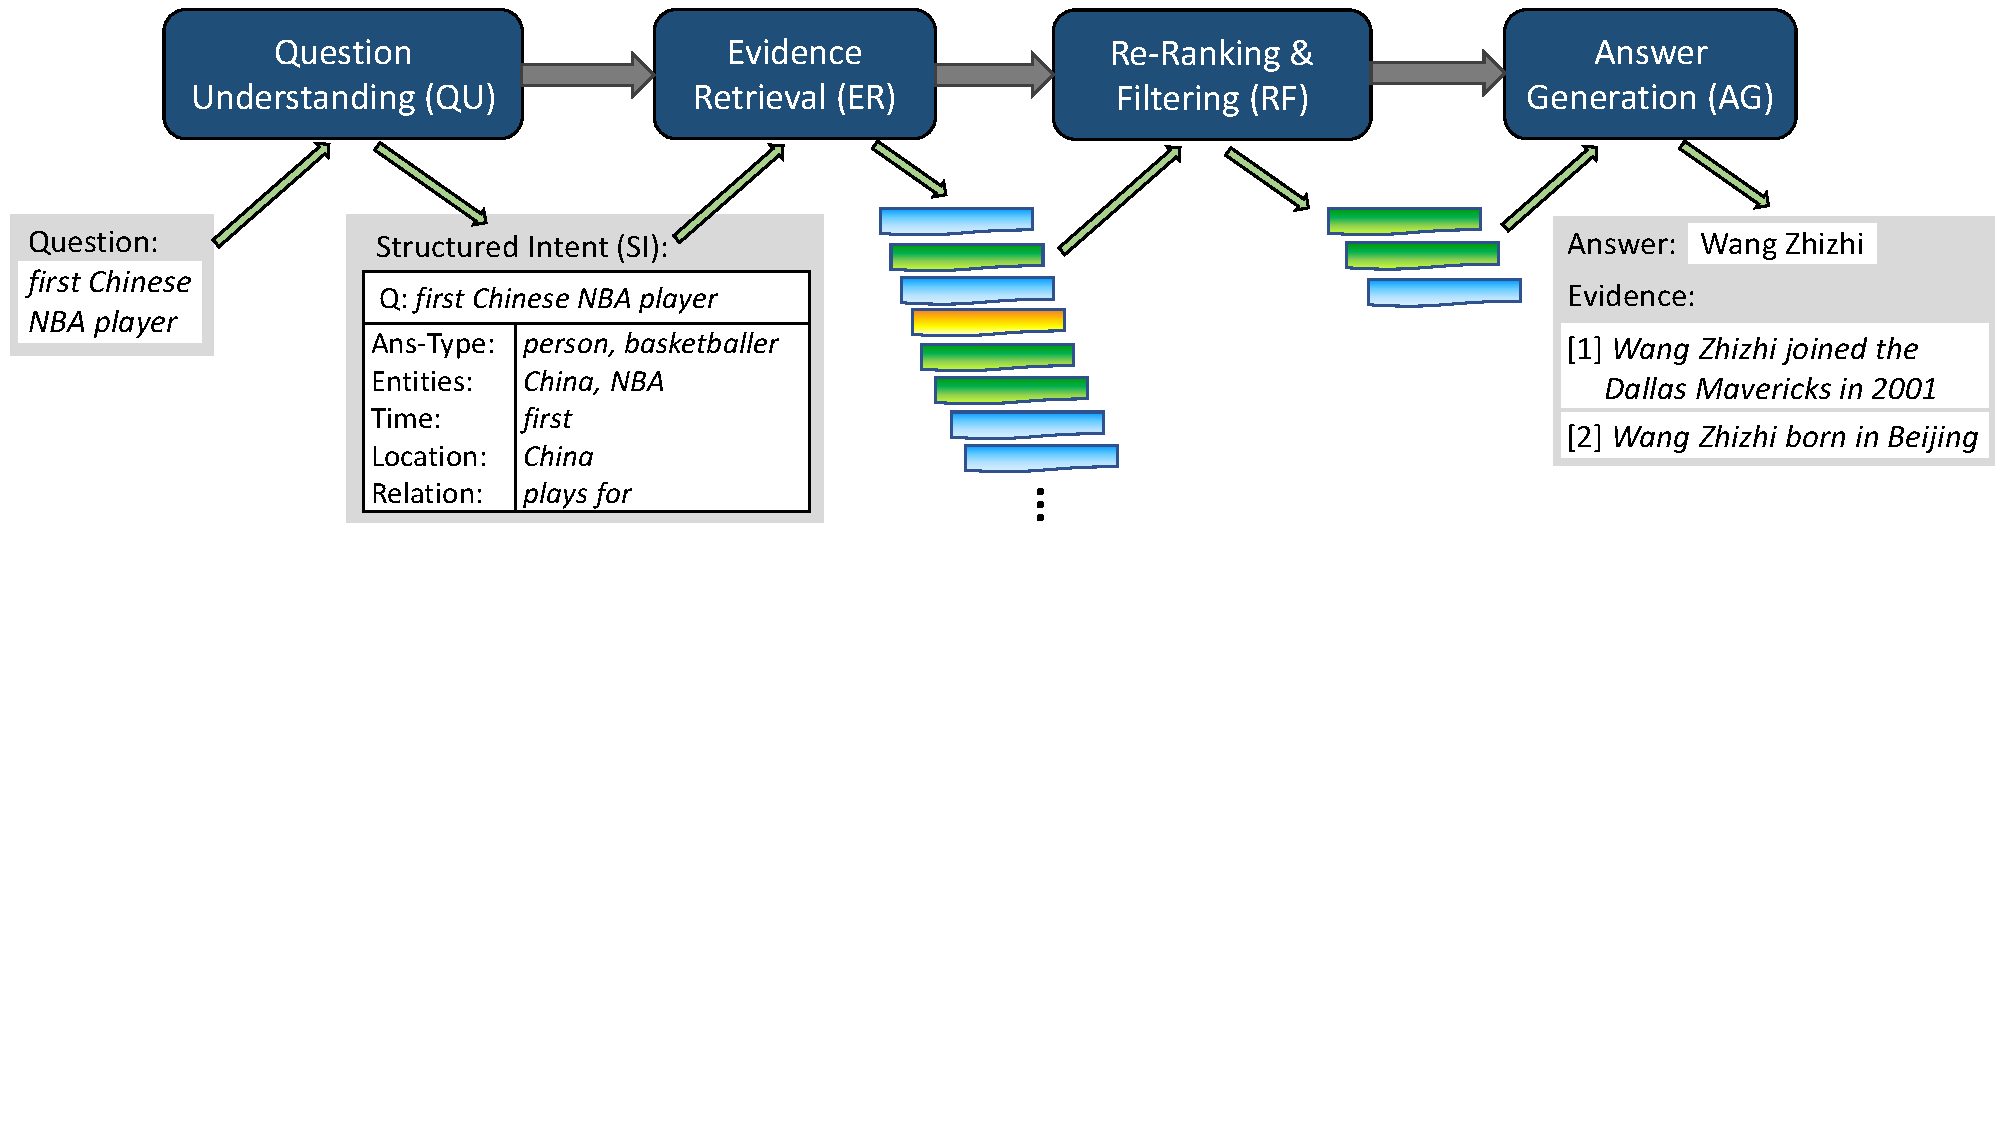
\includegraphics[width=\textwidth]{submissions/Gerhard2024/figures/compass-overview.pdf}
  \caption{Overview of the \method system.}
  \label{fig:compass-overview}
\end{figure}

% start with system overview
The \method system is a pipeline of four major stages, as illustrated in Figure \ref{fig:compass-overview}.
First, the input question is analyzed and decomposed, in order to compute a {\em structured intent (SI)} representation that will pass on to the subsequent steps, along with the original question. Second, the SI is utilized to retrieve pieces of evidence from different sources: text, KG and tables. 
Third, this pool of potentially useful evidence is filtered down, with iterative re-ranking, to arrive at a tractably small set of most promising evidence.
The final stage generates the answer from this evidence,
passing back the answer as well as evidence snippets for user-comprehensible explanation.

The second and fourth stage, Evidence Retrieval (ER) and Answer Generation (AG), are fairly standard. Such a two-phase architecture was called a retriever-reader architecture~\cite{Zhu-ODQA-survey:arxiv2021}. With a modern LLM replacing the earlier kinds of neural readers, this is the core of every RAG system~\cite{DBLP:journals/arXiv/abs-2312-10997}.

Stages 1 and 3 are unique elements of our architecture, judiciously introduced to improve both effectiveness (i.e., answer quality) and efficiency (i.e., computational cost).
Question Understanding (QU) provides the ER component with crisper and semantically refined input, and
the Re-Ranking \& Filtering (RF) stage is beneficial for
distilling the best evidence from the large pool of retrieved pieces.
The following subsections elaborate on the four stages of the pipeline, emphasizing the \method-specific steps QU and RF.



\subsection{Question Understanding (QU)}

% one par introducing the SI
To prepare the retrieval from different kinds of sources, including a KG, ad-hoc tables and text documents, it is useful to analyze and decompose the user question.
In this work, we aim to cast a question into a 
{\em structured intent (SI)} representation: essentially
a frame with faceted cues as slots, or equivalently, a concise set of key-value pairs. 
Figure \ref{fig:compass-overview} gives an idealized example for the question about the first Chinese NBA player. The facets or keys of potential interest here 
are:
\squishlist
\item {\em Ans-Type:} the expected answer type (or types when considering
different levels of semantic refinement), 
\item {\em Entities:} the salient entities in the question, and 
\item {\em Relation:} phrases that indicate which relation (between Q and A entities) the user is interested in. 
\squishend
\noindent In addition, as questions can have temporal or spatial aspects, the SI also foresees slots for:
\squishlist
\item {\em Time:} cues about answer-relevant time points or spans, including relative cues (e.g., ``before Covid'') and ordinal cues (e.g., ``first''), and
\item {\em Location:} cues about answer-relevant geo-locations.
\squishend

% discuss the spectrum of different SIs
\vspace{0.2cm}
\noindent The ideal SI for example question Q2 would look like:

\begin{quote}
{\em Ans-Type:} person, basketballer; {\em Entities:} China, NBA; {\em Time:} first;
{\em Location:} China; {\em Relation:} plays for.
\end{quote}

Note that the values for these slots can be crisp like entity names or dates, but they can also take the form of surface phrases. The SI purpose and value lie in the decomposition. In practice, many questions would only lead to a subset of faceted cues, leaving some slots empty. For the example in Figure \ref{fig:compass-overview}, an alternative SI could simply consist of

\begin{quote}
{\em Ans-Type:} person; {\em Entities:} China, NBA; {\em Time:} first.
\end{quote}

\noindent Even this simplified SI can be highly beneficial in guiding the subsequent evidence retrieval.

% sketch how an LM is trained to generate SIs 
To generate the SI from a user question, we employ a (small-scale) LM, specifically BART~\cite{DBLP:conf/acl/LewisLGGMLSZ20}, a Transformer-based auto-encoder with 140M parameters.\footnote{\url{https://huggingface.co/facebook/bart-base}}
BART is pre-trained for language representation; its power for our purpose comes from fine-tuning.
To this end, we generate (question, SI) pairs by using an instruction-trained LLM like GPT-4, with few-shot in-context learning (following our earlier work~\cite{Jia-FAITH:WWW2024}). 
Note that this is a one-time action; at inference-time we only use much smaller LMs.
The generated silver-standard pairs are then used to fine-tune BART.
In the experiments in this article, we leverage pre-existing collections of silver pairs, based on the training data of the CompMix benchmark~\cite{Christmann-CompMix:WWW2024}, 
comprising $3{,}400$ such pairs.


% outline value of SI for conversations
Although this paper focuses on single-shot questions, the \method architecture is also geared for conversational QA. In that setting, the SI can play an even bigger role, as (follow-up) questions are often formulated in a rather sloppy manner -- all but self-contained. For example, a conversation could start with a clear question {\em When did Wang Zhizhi join the NBA?}, followed a few dialog steps later, by a user utterance like {\em Which teams did he play for?} or simply {\em Which teams?}.
In such an informal conversation, the system needs to {\em contextualize} each user utterance based on the preceding turns in the dialog (e.g., inferring the relevant entities Wang Zhizhi and NBA from the conversational history).
For details on conversational QA, based on our architecture, see our earlier works~\cite{Christmann-CONVINSE:SIGIR2022,Christmann-Explaignn:SIGIR2023}.







%%%%%%%%%%%%%%%%%%%%%%%%%%%%%%%%%%%%%
\subsection{Evidence Retrieval (ER)}

The ER stage taps into a knowledge graph, a corpus of text documents, and a collection of web tables.
Specifically, for the experiments, we use the Wikidata KG,
all English Wikipedia articles, and all tables that are embedded in Wikipedia pages (incl. infoboxes, which can be seen as a special case of tables). 

% specifics: Clocq etc. - and the role of the SI
\vspace{0.2cm}
\noindent{\bf Retrieval from KG:}
To retrieve evidence from the KG, we utilize our earlier work
\clocq~\cite{Christmann-CLOCQ:WSDM2022}, which provides entity disambiguations and a relevant KG-subgraph for a given query.
Unlike most other works on QA-over-KG, \clocq fetches all KG-facts that are relevant for a given entity in a single step.
For example, when querying for
NBA players, it can traverse the KG neighborhood and pick up top teams, also considering so-called qualifier nodes in Wikidata which are often used for temporal scopes. 
As the disambiguation of entity names onto the KG can be tricky and noisy (e.g., China could be mapped to Chinese sports teams in all kinds of sports), \clocq considers several possible disambiguations~\cite{Christmann-CLOCQ:WSDM2022} (typically in the order of $10$ result entities).
The queries for \clocq are 
constructed by concatenating all slots of the question's SI.
For the example query about the first Chinese NBA player,
good result entities would be Dallas Mavericks, lists about NBA seasons, MVP awards etc., and their associated facts. These provide cues, but are likely insufficient to answer the question.


\vspace{0.2cm}
\noindent{\bf Retrieval from Text and Tables:}
The disambiguated entities returned by \clocq form anchors for tapping into text and tables.
\method first identifies 
relevant text documents and tables that refer to the anchor entities. With focus on Wikipedia, these are simply the articles for the respective entities. 
\method then constructs a keyword query that concatenates all available fields of the SI.
The query is evaluated against a linearized and verbalized representation (see below) of all sentences and all table rows in the selected documents.
This returns a set of sentences and 
and individual table rows, ranked by BM25 scores.


\vspace{0.2cm}
\noindent{\bf Evidence Verbalization:}
All results from the different data sources are uniformly treated by {\em linearizing} and {\em verbalizing} them
into token sequences. For KG results, the entity-centric triple sets are linearized via breadth-first traversal of the mini-graph starting from the entity node.
For tables, results are individual rows, which are contextualized by including labels from column headers and from the DOM-tree path of the article where the table comes from. For example, a table row about Wang Zhizhi playing for Dallas (Mavericks) in the 2000-2001 season, would be expressed as:

\vspace{0.05cm}
\hspace*{0.5cm} Wang Zhizhi / NBA Career / Season: 2000-2001, Team: Dallas, Games Played: 5 \dots
\vspace{0.05cm}

\noindent Finally, results from the text corpus are already in the form of token sequences, but we can additionally prefix these with the DOM-tree labels.
We can think of this entire pool of evidence as 
an on-the-fly corpus of potentially relevant pseudo-sentences, forming the input of the subsequent RF stage.


\vspace{0.2cm}
\noindent {\bf Result Ranking:}
Overall, the ER stage compiles a substantial set of evidence, possibly many thousands of entities, text snippets and table rows. Therefore, we practically restrict the pool to a subset of high-scoring pieces, like the top-$1000$.
For scoring, a simple BM25 model (a classical IR method) is applied. 
By default, we treat all evidence pieces uniformly with global scoring, no matter whether they come from KG, text or tables. 


\subsection{Re-Ranking and Filtering (RF)}

With a pool of top-$1000$ evidence pieces, we could invoke an LLM for answer generation. However, that would face a large fraction of noise (i.e., misleading evidence) and incur high costs of computation and energy consumption. 

For both of these reasons, we have devised light-weight techniques for iteratively reducing the top-$1000$ pieces to a small subset, say top-$30$ or top-$10$, that can be fed into an LLM at much lower cost (as LLM computations and pricing are at least linear in the number of input tokens). The difficulty is, of course, to do this without losing good evidence and reducing answer presence. Our techniques for this task are based on graph neural networks (GNNs)~\cite{Wu:IEEE2021} or cross-encoders (CEs)~\cite{Dejean:arxiv2024,Lin:MC2021}.

\myparagraph{GNN-based RF}
Given a large pool of evidence pieces from all sources, a bipartite graph is constructed:
\squishlist
\item {\em nodes} being evidence pieces or entities that occur in these pieces, and
\item {\em edges} connecting an evidence piece and an entity if the entity occurs in the evidence.
\squishend


The task for the GNN is to jointly score the evidence and the entity nodes in a multi-task learning setup. The latter are the {\em answer candidates}, and the evidence should give {\em faithful explanation} for an answer.
We build on our earlier work on explainable QA~\cite{Christmann-Explaignn:SIGIR2023}.

The node encodings are initialized with cross-encoder embeddings (see below) 
for node contents and the SI of the question. The inference iteratively adjusts the encodings based on message passing from neighboring nodes.
The GNN is trained via weak supervision from question-answer pairs:
evidence nodes are labeled as relevant if they are connected to
a gold answer.
More technical details are given in~\cite{Christmann-Explaignn:SIGIR2023}.

\method invokes the GNN in multiple rounds, iteratively reducing top-$k$ to top-$k^*$ nodes with $k^* \ll k$. In practice, we would typically consider two rounds: re-ranking top-$1000$ and pruning to top-100, and then reducing to top-30 or top-10, which are passed to the answer generation stage.
Note that this keeps the GNN at a tightly controlled size, so that its computational costs at inference-time are much smaller than those of an LLM.


\myparagraph{CE-based RF}
An alternative to the GNN inference is to employ a cross-encoder for scoring and re-ranking the evidence pieces.
These are transformers (typically with a small LM like BERT) that are fine-tuned for scoring the relatedness between a query and a document~\cite{Nogueira:arxiv2019}. In our case, the comparison is between the question SI and the evidence piece. In our experiments, we make use of two different cross-encoders, 
both trained on the MS-MARCO benchmark for passage retrieval~\cite{Bajaj:arxiv2018}, 
and fine-tuned on the respective benchmark (leveraging the same weak supervision data as for the GNNs),
the difference being in model size.\footnote{\url{https://huggingface.co/cross-encoder/ms-marco-MiniLM-L-4-v2} and\\ \url{https://huggingface.co/cross-encoder/ms-marco-MiniLM-L-6-v2}}
We use the smaller model to reduce top-$1000$ to top-100, and the larger model to go further down from top-100 to top-30.




%%%%%%%%%%%%%%%%%%%%%%%%%%%%%%%%%%%%%

\subsection{Answer Generation (AG)}

The last stage follows mainstream practice to invoke an LLM in a retrieval-augmented manner.
We call a `small-scale` LLM, specifically a fine-tuned LlaMA-3.1 model (8B-Instruct)\footnote{\url{https://huggingface.co/meta-llama/Llama-3.1-8B-Instruct}}, with a prompt \footnote{The specific prompt is \phrase{SI: \textless\texttt{concatenated SI}\textgreater \hspace{0.1cm} Evidence: \textless\texttt{evidence pieces}\textgreater}.}
consisting of:

\squishlist
\item the concatenated SI of the original question, and
\item the top-30 (or other top-$k^*$ with small $k^*$) evidence pieces.
\squishend

By the previous down-filtering of the original pool of evidence pieces, this last step has affordable cost in terms of computation time and energy consumption.

\vspace{0.2cm}
\noindent{\bf Fine-Tuning the LLM:}
We considered adding an instruction to the prompting, such as {\em ``answer this question solely based on the provided evidence snippets''}.
However, this turned out to be ineffective.
The reason why the model works well without such instructions is our task-specific fine-tuning.
We perform this by running the training data of benchmarks through the \method pipeline,
and training the AG stage with the top-30 evidence pieces as input.
Thus, the fine-tuning makes the model learn the role of evidence for RAG-based QA.

\vspace{0.2cm}
\noindent{\bf Explanations:}
The top-30 evidence pieces can be used to provide users with explanation of answers.
Optionally, these could be reduced further for comprehensibility.
Alternatively, we can fine-tune the LLM to provide both answers and concise explanations.
Since we can infer which evidences in the input mention the annotated ground-truth answers,
our method could be fine-tuned to provide such \textit{answering evidences} as well (cf.~\cite{Gao-citations:emnlp2023}).

\label{sec:exp}
\section{Experiments}


\label{setup}
\subsection{Experimental setup}


%%% BENCHMARKS
\myparagraphnospace{Benchmarks} We run experiments on three benchmarks with different characteristics of questions.

\squishlist
    \item \textbf{\compmix}.
    \compmix~\cite{Christmann-CompMix:WWW2024} is a benchmark which was specifically designed for evaluating QA systems operating over heterogeneous sources. The dataset has $9{,}410$ questions, out of which $2{,}764$ are used for testing.
    Answers are crisp entity names, dates, or other literals.
    
    \item \textbf{\crag}.
    We further evaluate on a subset of the \crag~\cite{Yang-CRAG} dataset, which was recently released as a testbed for RAG-based QA systems.
    We utilize the same pipeline and sources as outlined in Section~\ref{sec:method}, without using the web snippets or APIs provided with \crag. This way we focus on entity-centric questions that do not require access to live web data (e.g., news feeds), and disregard cases where the results would be up-to-date quantities.
    This restricts the test data to $436$ entity-centric questions, still enough for a proof of concept.
    
    \item \textbf{\timequestions}.
    To showcase the generalizability of our pipeline, we conduct experiments on~\timequestions~\cite{Jia-TimeQuestions},
    a benchmark for temporal QA. The dataset requires temporal understanding and reasoning, which are well-known limitations of
    LLMs~\cite{Dhingra-time-aware-LLM:TACL2022}. \timequestions has 16{,}181 questions (3{,}237 for testing).
\squishend

Typical examples for the questions in these three benchmarks are:

\begin{quote}
\compmix: \utterance{Which player won the most number of Man-of-the-Match titles in the FIFA world cup of 2006?}\\
 \indent \crag: \utterance{What was the worldwide box office sales for little hercules?}\\ 
  \indent \timequestions: \utterance{Which club did Cristiano Ronaldo play for before joining Real Madrid?}
\end{quote}

%%% BASELINES
\myparagraph{Baselines} As competitors or reference points to \method, we study the performance of the following methods:

\squishlist
    \item \textbf{Generative LLMs}.
    We compare \method against out-of-the-box LLMs: \textbf{\gptthree} (\texttt{text-davinci-003}), \textbf{\gptfour} (\texttt{gpt-4}) 
    and \textbf{\llama} (\texttt{meta-llama/Llama-3.1-8B-Instruct}).
    The same prompt is used for all LLMs, consistent with previous work~\cite{Christmann-CompMix:WWW2024, Zhang-Spaghetti:ACL2024}:
    \phrase{Please answer the following question by providing the crisp answer entity, date, year, or numeric number. Q: \textless\texttt{question}\textgreater}.
    

    \item \textbf{Heterogeneous QA methods}.
    \convinse~\cite{Christmann-CONVINSE:SIGIR2022}, \unikqa~\cite{Oguz-UniK-QA:NAACL2022}, \explaignn~\cite{Christmann-Explaignn:SIGIR2023}
    are QA methods designed to integrate heterogeneous sources: text, tables and KG. All of these  integrate the exact same sources as \method.

    
    \item \textbf{\textsc{State-of-the-art}}.
    For \compmix and \timequestions, we also compare against state-of-the-art methods from the literature: \spaghetti~\cite{Zhang-Spaghetti:ACL2024} and \textsc{Un-Faith}~\cite{Jia-FAITH:WWW2024}, which are among the best performing systems.
    
Results are taken from the literature whenever applicable.
On \crag, we use the models trained on \compmix for \method and heterogeneous QA baselines.
\squishend



%%% METRIC(S)
\myparagraph{Metrics}
We measure \textit{precision at 1} (\textbf{P@1}) as our main metric~\cite{RoyAnand:MC2021} on all benchmarks.
On \crag, we manually annotate answer correctness, as the ground-truth answer formats vary (e.g., entity name variants, lists, sentences).

We also compute the number of neural parameters aggregated over all sub-modules (\textbf{\#Parameters}).
Parameter counts for GPT-models are taken from~\cite{Minaee-LLM-survey}
(\gptfour might have less active parameters during inference).

For further analysis we measure \textit{answer presence} (\textbf{AP@k}),
i.e. whether the answer is present in the top-$k$ ranked evidence pieces,
and \textit{mean reciprocal rank} within the top-$k$ evidences (\textbf{MRR@k}).

%%% CONFIG
\myparagraph{Configuration}
Our implementation uses the \texttt{Llama3.1-8B-Instruct} model for the AG stage.
For the QU, ER and RF stages
we adopt code from the \explaignn project.\footnote{\url{https://explaignn.mpi-inf.mpg.de}}
For the ER stage, we use \clocq, setting its specific parameters to $k=10$ and $p=1{,}000$.

As default, we use the GNN technique for the RF stage.
For efficiency, we use light-weight models for initializing
the GNN encoders -- the same models used for the CE-based RF.\footnote{\url{https://huggingface.co/cross-encoder/ms-marco-MiniLM-L-4-v2} and\\\url{https://huggingface.co/cross-encoder/ms-marco-MiniLM-L-6-v2}}
The GNNs are trained for $5$ epochs with an epoch-wise evaluation strategy,
i.e. we choose the model with the best performance on the respective dev set.
We train the GNNs on graphs with a maximum of $100$ evidence and $400$ entity nodes (as scored by BM25).
During inference, the first GNN is applied on graphs with $1{,}000$ evidence and $4{,}000$ entity nodes, shrinking the pool of evidence pieces to the top-$100$.
The second GNN then runs on graphs with $100$ evidence and $400$ entity nodes.
The factor of 4 entities per evidence (on average) holds sufficient for the observed data,
and enables batched inference.
Other parameters are kept as is.

The AG model, based on \texttt{Llama3.1-8B-Instruct}, is 
fine-tuned
for $2$ epochs with a warm-up ratio of $0.01$ and a batch size of $8$, again with an epoch-wise evaluation strategy.
Other parameters are set to the default Hugging Face
training parameters.\footnote{\url{https://huggingface.co/docs/transformers/v4.46.2/en/main_classes/trainer\#transformers.TrainingArguments}}





\subsection{Main results}
%%% MAIN TABLE
\myparagraphnospace{\method is competitive on all benchmarks}
Main results of our experiments are shown in Table~\ref{tab:main-res}.
First of all, we note that \method achieves competitive performance across all three benchmarks.

On \compmix, baselines for heterogeneous QA and \llama perform similarly,
whereas GPT-based LLMs can answer more than $50$\% of the questions correctly.
\method exhibits substantially higher performance, on par with
the state-of-the-art method \textsc{Spaghetti}~\cite{Zhang-Spaghetti:ACL2024}
(which is based on \gptfour).

On the \crag dataset, P@1 drops for all methods except for \gptfour. 
The benchmark includes realistic questions,
which can be ambiguous/confusing (\phrase{who was the director for the report?}),
on ``exotic'' entities with answers in social media (\phrase{how many members does the teknoist have?}),
or require up-to-date information (\phrase{when did chris brown release a song or album the last time?}),
and other cases that are challenging for all methods.

Finally, \method establishes new state-of-the-art performance on the \timequestions benchmark.
Interestingly, all of the tested LLMs show greatly reduced performance on this benchmark,
which inherently requires temporal understanding and reasoning
-- a known weakness of stand-alone LLMs.


\begin{table} [h]
    \centering
    \newcolumntype{G}{>{\columncolor [gray] {0.90}}c}
    \begin{tabular}{l G G G c}
        \toprule
            \textbf{Method $\downarrow$ / Benchmark $\rightarrow$} & \textbf{\compmix}  & \textbf{\crag} & \textbf{\timequestions} & \textbf{\#Parameters} \\ 
        \midrule
            \textbf{\gptthree} 
            & $0.502$ &   $-$ & $0.224$ & $175{,}000$ M  \\
            % #params from https://arxiv.org/pdf/2402.06196

            \textbf{\gptfour}
            & $0.528$ &   $\mathbf{0.633}$ & $0.306$ & $1{,}760{,}000$ M \\
            % #params from https://arxiv.org/pdf/2402.06196

            \textbf{\llama~\cite{Touvron-LLaMA}} (8B-Instruct)
            & $0.431$ &   $0.385$ & $0.178$ & $8{,}030$ M  \\
            % #params from Huggingface (8,030,257,152)
        \midrule
            \textbf{\convinse~\cite{Christmann-CONVINSE:SIGIR2022}}
            & $0.407$  &   $0.298$ & $0.423$  & $362$ M \\
            % FiD: 222,903,936 + BART (SR-generation): 139,420,416 = 362,324,352 (python explaignn/question_understanding/structured_representation/get_num_params.py)

            \textbf{\unikqa~\cite{Oguz-UniK-QA:NAACL2022}}
            & $0.440$ &   $0.280$ & $0.424$ & $223$ M  \\
            % FiD: 222,903,936 (python explaignn/heterogeneous_answering/fid_module/FiD/get_num_params.py)
    
            \textbf{\explaignn~\cite{Christmann-Explaignn:SIGIR2023}} 
            & $0.442$ &   $0.303$ & $0.525$  & $328$ M \\
            % BART (SR-generation): 139,420,416 + 2GNNs: 94520832 + 93930240 = 327,871,488

        \midrule 
            \textbf{\textsc{State-of-the-art}}
            & $\mathbf{0.565}$ 
            & $-$
            & $0.571$  & $-$ \\

            & (\textsc{Spaghetti}~\cite{Zhang-Spaghetti:ACL2024})
            & 
            & (\textsc{Un-Faith}~\cite{Jia-FAITH:WWW2024}) &  \\

        \midrule
            \textbf{\method (ours)}
            & ${0.564}$ &   $0.362$ & $\mathbf{0.754}$  & $8{,}218$ M \\
            % BART (SR-generation): 139,420,416 + LLaMA: 8,030,257,152 + GNNs: 25,670,016 + 22,268,928 =  8,217,616,510
        \bottomrule
    \end{tabular} 
    \vspace*{-0.2cm}
    \caption{End-to-end P@1 of \method and baselines on three benchmarks. Results for \gptthree and \gptfour are taken from the literature~\cite{Christmann-CompMix:WWW2024, Jia-FAITH:WWW2024}. \gptthree is not accessible anymore, hence no results on \crag.
    }
    \label{tab:main-res}
\end{table}





%%% ANSWER SOURCES
\myparagraph{Integration of heterogeneous sources is vital}
\method integrates evidence from text, KG and tables into a unified framework.
We aim to better understand how this affects the answering performance of the method.
Table~\ref{tab:sources} shows end-to-end answering performance of \method
with different combinations of the input sources.
The results clearly indicate that all types of sources contribute, with option Text+KG+Tables performing best,
with a large margin over tapping only single source types.

\begin{table} [t] 
    \centering
    \newcolumntype{G}{>{\columncolor [gray] {0.90}}c}
    \newcolumntype{H}{>{\setbox0=\hbox\bgroup}c<{\egroup}@{}}
    	\begin{tabular}{l G G G H H H c c c} 
        \toprule
            \textbf{Benchmark $\rightarrow$}
                & \multicolumn{3}{G}{\textbf{\compmix}} 
                & \multicolumn{3}{H}{\textbf{\crag}}
                & \multicolumn{3}{c}{\textbf{\timequestions}} \\ 
        \midrule
            \textbf{Input sources $\downarrow$ / Metric $\rightarrow$}
                & \textbf{P@1} & \textbf{AP@100}  & \textbf{AP@30}
                & \textbf{P@1} & \textbf{AP@100}  & \textbf{AP@30}
                & \textbf{P@1} & \textbf{AP@100}  & \textbf{AP@30} \\
            \midrule
                \textbf{Text}           &  $0.455$  &  $0.563$  &  $0.531$ &  $?$  &  $?$  &  $?$ &  $0.539$  &  $0.515$  &  $0.487$   \\
                \textbf{KG}             &  $0.481$  &  $0.677$  &  $0.637$ &  $?$  &  $?$  &  $?$ &  $0.724$  &  $0.701$  &  $0.674$   \\
                \textbf{Tables}         &  $0.432$  &  $0.501$  &  $0.482$ &  $?$  &  $?$  &  $?$ &  $0.536$  &  $0.347$  &  $0.328$   \\
            \midrule
                \textbf{Text+KG}        &  $0.537$  &  $0.749$  &  $0.706$ &  $?$  &  $?$  &  $?$ &  $0.745$  &  $\mathbf{0.776}$  &  $0.748$   \\
                \textbf{Text+Tables}    &  $0.503$  &  $0.632$  &  $0.594$ &  $?$  &  $?$  &  $?$ &  $0.567$  &  $0.578$  &  $0.549$   \\
                \textbf{KG+Tables}      &  $0.524$  &  $0.728$  &  $0.692$ &  $?$  &  $?$  &  $?$ &  $ 0.743$  &  $0.731$  &  $0.703$   \\
            \midrule
                \textbf{Text+KG+Tables}    &  $\mathbf{0.564}$  &  $\mathbf{0.759}$  &  $\mathbf{0.724}$ &  $?$ &  $?$  &  $?$ & $\mathbf{0.754}$    & $\mathbf{0.776}$  &  $\mathbf{0.749}$   \\
            \bottomrule
    \end{tabular}
    \vspace*{-0.2cm}
    \caption{Answer presence and answering precision of \method with different combinations of input sources (on the respective test sets).}
    \label{tab:sources}
\end{table}




\subsection{Analysis}

%%% TOP-K vs. 3xTOP-(K/3)
\myparagraph{Unified retrieval enhances performance}
In the RF stage, we re-rank and filter evidence from different source types,
and feed the unified top-\textit{k}* into the AG stage.
We conduct a comparison in which we consider
the top-$10$ evidence pieces from each source type individually. This gives equal influence to KG, text and tables, whereas our default is based on global ranking.
Table~\ref{tab:unified-retrieval} shows the results for this analysis, showing our default choice performs better.
The reason is that different questions require different amounts of evidence from each of the source types.

\begin{table} [t] 
    \centering
    \newcolumntype{G}{>{\columncolor [gray] {0.90}}c}
    \newcolumntype{H}{>{\setbox0=\hbox\bgroup}c<{\egroup}@{}}
    	\begin{tabular}{l G G H H} 
        \toprule
            \textbf{Input evidences $\downarrow$ / Metric $\rightarrow$} & \textbf{P@1} & \textbf{AP@30}  & \textbf{\crag} & \textbf{\timequestions} \\ 
            \midrule
                \textbf{Top-30 Text+KG+Tables (ours)}             &  $\mathbf{0.574}$  &  $\mathbf{0.710}$  &  $-$  &  $-$   \\
                \textbf{Top-10 Text + Top-10 KG + Top-10 Tables}        &  $0.560$    &  $0.709$  &  $-$  &  $-$   \\
            \bottomrule
    \end{tabular}
    \vspace*{-0.2cm}
    \caption{Answer presence and precision
    of \method for different choices of top-30 
    (on \compmix dev set).}
    \label{tab:unified-retrieval}
\end{table}


%%% NUMBER OF EVIDENCES
\myparagraph{\method works well with small amounts of evidence}
We investigate the 
influence of 
the number of evidence pieces
fed into the AG stage, varying it from $5$ to $100$.
Results are shown in Figure~\ref{fig:res-num-evidences}.
As the curve shows, there is a sharp increase in precision as we add evidence up to 30 or 40 pieces, which is around our default of top-30. This indicates that a certain amount of evidence is needed, to overcome the inherent noise and arrive at sufficient answer presence. 
As we increase the amount of evidence further, we observe a saturation effect, and eventually a degration of performance. Too much evidence not only has diminishing returns, but can actually be confusing for the AG stage. This reconfirms our heuristic choice of top-30: enough for good answering while keeping computational costs reasonably low.


\begin{figure}[t]
    \centering
    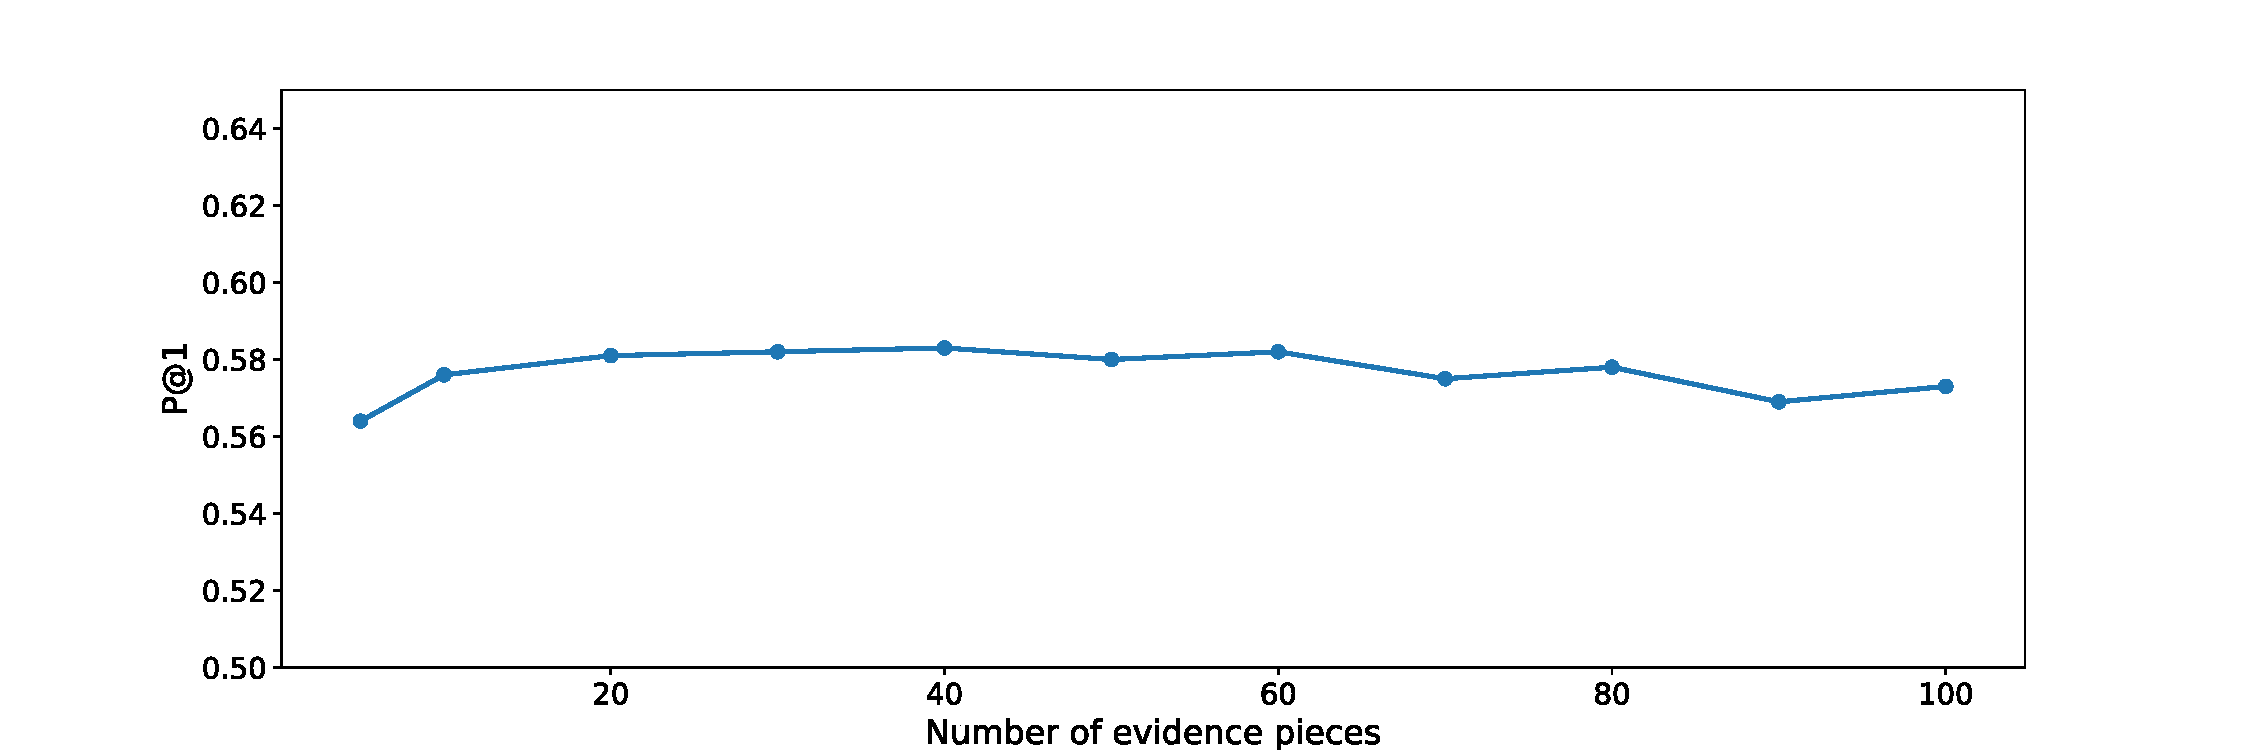
\includegraphics[width=0.8\textwidth]{submissions/Gerhard2024/figures/p_at_1-line_with_evidences.pdf}
    \vspace*{-0.2cm}
    \caption{Performance of \method on the \compmix dev set with different numbers of evidence.}
    \label{fig:res-num-evidences}
    \vspace*{-0.2cm}
\end{figure}



%%% ABLATION
\myparagraph{Ablation study on re-ranking} For more insight on the possible configurations of the RF stage, we conducted an ablation study with different options, including solely relying on the initial BM25 scoring without explicit re-ranking. The results are shown in Table \ref{tab:ablation2}. We observe that the iterative reduction in two steps is slightly better than the single-step variants (going down from top-1000 to top-30 in one RF step). Between the two options of using a GNN or a CE, the differences are negligible. A notable effect is that our RF techniques retain the answer presence at a very high level, only a bit lower than for the initial top-1000. 
The last two rows of Table \ref{tab:ablation2} demonstrate that RF is crucial: without explicit re-ranking, the technique of just picking smaller top-$k$ from the original BM25 model leads to substantial degradation in both answer presence and precision. 


\begin{table} [t] \small
    \centering
    \newcolumntype{G}{>{\columncolor [gray] {0.90}}c}
    \newcolumntype{H}{>{\setbox0=\hbox\bgroup}c<{\egroup}@{}}
    	\begin{tabular}{l G H G G G} 
        \toprule
            & \multicolumn{5}{G}{\textbf{\compmix} (dev set)} \\
        \midrule
            \textbf{RF Method $\downarrow$ / Metric $\rightarrow$} & \textbf{P@1} & \textbf{AP@1000} & \textbf{AP@100}  & \textbf{AP@30} & \textbf{MRR@100} \\ 
        \midrule
            \textbf{GNN: 1000 $\rightarrow$ 100 $\rightarrow$ 30}             &  $\mathbf{0.574}$  & $0.760$ &  $0.738$  &  $0.710$  &  $\mathbf{0.572}$  \\
            \textbf{CE: 1000 $\rightarrow$ 100 $\rightarrow$ 30}          &  $0.573$  & $0.760$  &   $\mathbf{0.740}$ &  $\mathbf{0.721}$   &  $0.553$   \\
        \midrule
            \textbf{GNN: 1000 $\rightarrow$ 30} &  $0.567$  & $?$  &   $n/a$ &  $0.710$   &  $0.567$   \\
         \textbf{CE: 1000 $\rightarrow$ 30} &  $0.570$  & $0.760$  &   $n/a$ &  $0.715$   &  $0.558$   \\
            \midrule
           \textbf{BM25: 100 (w/o GNN or CE)} &  $0.490$ & $0.760$  &  $0.652$  &  $n/a$  &  $0.259$ \\       
            \textbf{BM25: 30 (w/o GNN or CE)} &  $0.468$  & $0.760$  &  $n/a$ &  $0.534$   &  $0.259$   \\
            \bottomrule
    \end{tabular}
    \vspace*{-0.2cm}
    \caption{Ablation study for different RF strategies of \method on the \compmix dev set. The answer presence in the RF input with top-$1000$ evidence pieces is $0.760$.}
    \label{tab:ablation2}
\end{table}



\myparagraph{Quality of SI}
To assess the quality and robustness of the Structured Intents, we
inspected a sample of questions and their SIs.
Table~\ref{tab:question-SI-examples} gives three anecdotic examples.
We show SIs generated by \method, which makes use of the pre-existing collection from the \compmix benchmark for training.
This training data was obtained via different heuristics, 
which can be a limiting factor when user intents become more complex.

Therefore, we also looked at SIs derived via in-context learning (ICL) using \gptfour with $5$ handcrafted examples.
As shown in our earlier work on temporal QA~\cite{Jia-FAITH:WWW2024},
such data can be used for training smaller models (e.g., BART),
which can greatly boost the completeness and overall quality of the generated SIs.

From the sampled set, we observed that the ICL-based SIs are more
complete with all slots filled, whereas the BART-based SIs focused more
on the main slots Answer-type, Entities and Relation.
However, both approaches achieve very high quality in filling the slots,
capturing the user's information need very well.

Interestingly, when questions get complicated, with nested phrases, 
the ICL-based variant succeeds in decomposing the questions, based on only $5$ ICL examples.
For example, for the question {\em ``which German state had the most Corona-related death cases in the first year after the outbreak?''}
the Time slot becomes {\em ``first year after Corona outbreak''},
which can be resolved to identify the temporal scope.
In general, we believe that such question decomposition, beyond simple temporal constraints,
would be an interesting theme for future work.

\begin{table} [t] 
    \centering
    \small
    \newcolumntype{G}{>{\columncolor [gray] {0.90}}c}
    \newcolumntype{H}{>{\setbox0=\hbox\bgroup}c<{\egroup}@{}}
    \resizebox*{\textwidth}{!}{
        \begin{tabular}{p{6cm}|p{6cm}|p{6cm}} 
        \toprule
            \textbf{Question} & \textbf{Current SI by \method} & \textbf{SI via ICL} \\
        \midrule
        \textit{what was disneys first color movie?}
            & Ans-Type: \textit{animated feature film} & Ans-Type: \textit{film, animated film} \\
            & Entities: \textit{disneys} & Entities: \textit{Disney} \\
            & Relation: \textit{was first color movie} & Relation: \textit{first color movie} \\
            &  & Time: \textit{first} \\
        \midrule
        \textit{at the oscars, who won best actor in 2018?}
            & Ans-Type: \textit{human} & Ans-Type: \textit{person, actor} \\
            & Entities: \textit{at the oscars} & Entities: \textit{Oscars, 2018} \\
            & Relation: \textit{who won best actor in 2018} & Relation: \textit{won best actor} \\
            &  & Time: \textit{2018} \\
        \midrule
        \textit{which German state had the most Corona-} & Ans-Type: \textit{state} & Ans-Type: \textit{location, state} \\
        \textit{related death cases in the first year after} & Entities: \textit{Germany, Corona} & Entities: \textit{Germany, Corona-related deaths} \\
        \textit{the outbreak?} & Relation: \textit{which state had the most related} & Relation: \textit{highest count of death cases} \\
        & \textit{death cases in the first year after the out-}  & Location: \textit{Germany} \\
            & \textit{break}  & Time: \textit{first year after Corona outbreak} \\
        \bottomrule
    \end{tabular}
    }
    \vspace*{-0.2cm}
    \caption{Examples for pairs of question and generated SI.}
    \label{tab:question-SI-examples}
\end{table}




%%% REFRAIN FROM ANSWER
\myparagraph{Refraining from answering}
%%% Searched for: "generated_answer I" (with I being the full word, not partial) in the generated answers of LLaMA
%%% yields 245 results out of 2764 questions on CompMix
%%% yields 1270 results out of 3237 questions on TimeQuestions
We can train our model to refrain from answering in scenarios
where the provided evidence does not contain an answer to the question.
Specifically, during training, when the answer is not present in the evidence,
we change the target answer to {\em unknown}. This variant is referred to as \method {\em (faithful)}.

We measure the ratio of questions for which {\em unknown} is provided as answer,
and the P@1 restricted to questions that are answered.
The accuracy of refraining from answering is measured as well,
based on whether the answer is present in the evidence or not.
We conduct this experiment on \compmix and \timequestions,
for which we can compute answer presence exactly.
We also compute results for \llama, which is already instructed 
with the option to answer ``don't know''.
Table~\ref{tab:refrain-from-answer} shows the results.
For \compmix, we observe that \method has high accuracy on refraining when appropriate,
whereas \llama tends to be overconfident with a very small rate of {\em unknowns}, leading to incorrect answers.

\begin{table} [t] \small
    \centering
    \newcolumntype{G}{>{\columncolor [gray] {0.90}}c}
    \newcolumntype{H}{>{\setbox0=\hbox\bgroup}c<{\egroup}@{}}
    	\begin{tabular}{l G G G G c c c c} 
        \toprule
            & \multicolumn{4}{G}{\textbf{\compmix}} & \multicolumn{4}{c}{\textbf{\timequestions}} \\
            \midrule
            \textbf{Metric $\rightarrow$} & \textbf{P@1}  & \textbf{P@1} & \textbf{Refrain} & \textbf{Refrain} & \textbf{P@1}  & \textbf{P@1} & \textbf{Refrain} & \textbf{Refrain} \\ 
            \textbf{Method $\downarrow$} &                 & \textbf{(answered)} & \textbf{rate} & \textbf{accuracy} &                 & \textbf{(answered)} & \textbf{rate} & \textbf{accuracy} \\ 
            \midrule
                \textbf{\llama}             &  $0.431$  &  $0.471$  &  $0.089$  &  $n/a$  &  $0.177$  &  $0.276$  &  $0.392$  &  $n/a$  \\
                \textbf{\method (faithful)}           &  $0.497$  &  $0.713$  &  $0.303$  &  $0.838$ &  $0.597$  &  $0.804$  &  $0.257$  &  $0.864$  \\
            \bottomrule
    \end{tabular}
    \vspace*{-0.2cm}
    \caption{
        Performance of \method with option to refrain from answering (``don't know'').
    }
    \label{tab:refrain-from-answer}
\end{table}

\label{sec:disc}
\section{Insights, Limitations, and Challenges}


\noindent{\bf Benchmark Performance.} Our method, RAG-based \method with an 8B LLaMA model, outperforms much larger LLMs like \gptfour on two of the three benchmarks, with a very large margin for temporal questions. Obviously, pre-trained LLMs have only limited sense of properly positioning ``remembered’’ facts on the timeline even with training data that exceeds ours by several orders of magnitude. This confirms our intuition that LLMs alone are not good at ``recalling’’  higher-arity relations that require combining distant pieces of evidence. This is a sweet spot for RAG. Only for 
the \crag benchmark, \method is substantially inferior to a full-blown LLM. This is likely due to the nature of the questions: not necessarily the complexity of the information needs, but the need for more web sources (beyond what our experiments tap into).

\vspace{0.2cm}
\noindent{\bf Cost/Performance Ratio.} The most important take-away from our experiments is that \method achieves its competitive performance at a much lower cost than the full LLMs. Assuming that the consumed GFlops are proportional to the number of model parameters, \method achieves a cost reduction by a factor of 200x for \gptthree and 2000x for \gptfour. This does not only mean less computation, but also a massively lower electricity bill and climate impact.  

\vspace{0.2cm}
\noindent{\bf Role of Question Understanding.} We did not systematically investigate the influence of the Structured Intent in the \method pipeline. However, the comparison to the big GPT models reflects the role of the SI, as we prompt the GPT models in their natural mode with the original questions. The linearized sequence of available SI slots does not always have major advantages, but there are enough cases where specific facets provide crucial cues. This holds especially for the Entities slot, as this drives the gathering of evidence in the ER stage (cf.~\cite{Christmann-CONVINSE:SIGIR2022}, and for the Time slot, as these cues are often decisive for temporal questions (cf.~\cite{Jia-FAITH:WWW2024}).

\vspace{0.2cm}
\noindent{\bf Role of Re-Ranking.} As our ablation studies show, merely using top-$k$ evidence from an initial BM25-style ranking does not provide good performance. Also, there seems to be sweet spot in the choice of $k$: we need enough evidence for connecting the dots if the question requires multiple pieces of information, or for corroborating candidates if the question finds many useful but noisy pieces. In the experiments, $k=30$ turns out to be good choice; much lower $k$ results in insufficient evidence, and much larger $k$ leads to saturation and ultimately degrading performance. Our argument for iteratively shrinking the candidate set in multiple rounds of re-ranking is substantiated in our experiments, but the gain of doing this, compared to GNN- or CE-based re-ranking from 1000 to 30, is not big. More research is called to better understand the role of ranking in RAG. 

\vspace{0.2cm}
\noindent{\bf Limitations of Evidence Retrieval.}
For ER, we adopted more or less standard techniques. The results showed very good answer presence, in the order of 75\% in the top-100 or even top-30. An important case where this is insufficient are questions that require aggregating information over a large number of evidence pieces. An example is asking for the life-time total of 3-point scores of the basketball player Dirk Nowitzki.
This requires collecting a set of per-season tables with NBA player statistics, but also other web sources with numbers for his career before he joined the NBA (including his youth teams).
Of course, there are sometimes shortcuts like a Wikipedia article or biography mentioning the total number, but this cannot be universally assumed. The bottom line is that ER should be reconsidered as well, striving to improve the recall dimension.

\vspace{0.2cm}
\noindent{\bf Limitations of Answer Generation.}
For AG, we simply rely on a LLM,
using it as an extractor (``reader'') from the given evidence. Despite the wide belief that LLMs can perform deep
reasoning over many pieces of evidence, our experience is that the extraction works only well – robustly and faithfully – for relatively simple questions with a few multi-hop joins or simple aggregation over a few pieces. However, complicated questions such as asking for the top-100 NBA players with the largest number of life-time 3-point scores (again including their pre-NBA careers) are currently out of scope and will likely remain so for quite some time. This offers many opportunities for pushing the envelope further.

\vspace{0.2cm}
\noindent{\bf Trust in Data Sources.}
In our experiments, we considered all heterogeneous sources as trustworthy and unbiased. With focus on Wikidata and Wikipedia, this assumption has been well justified. In the wild, however, input data for RAG-based systems likely exhibit a wide spectrum of quality issues, in terms of stale information, biased positions, or simply false statements. Identifying trustworthy and up-to-date evidence and dealing with conflicting data, has been explored in other contexts (e.g., for KG curation~\cite{Dong-Trust:PVLDB2015}), but remains a major challenge for RAG-based QA.


\vspace{0.2cm}
\noindent{\bf Open Challenges and Future Work.} The best-performing methods in our experiment, mostly \method, reach P@1 values of 56\% for \compmix and 75\% for \timequestions. 
For the latter, the answer presence in the top-100 is only slightly higher; so the AG stage hardly misses anything.
However, for \compmix, the answer presence is 75\% -- much higher than what our system can actually answer. Obviously, closing this gap is a major direction to pursue, with focus on the RF and AG stages. However, missing one fourth of the answers completely in the top-100 pool, is a big problem as well. This requires improving recall at the ER stage, possibly with better guidance by the QU, which in turn needs more sources beyond the scope of our experiments (currently limited to Wikidata and Wikipedia). 

In general, we need to think beyond this kind of ``benchmark mindset’’. Even if we reached 80\% or 90\% precision and recall, we would still have a substantial fraction of questions that are answered incorrectly
or not at all. 
The remaining errors may not be a problem for chatbots, but they would be a showstopper for the deployment of mission-critical applications in business or science. We believe that this big gap is a shortcoming of {\em all methods}, not an issue that comes from the data alone. For trivia-style QA, as looked at in this paper, a smart human in ``open book’’ mode and no time limitation should be able to properly answer practically all questions, just by reading pieces of web contents and putting things together. Neither LLMs nor state-of-the-art RAG are the final solution; substantial research and creative ideas are needed to further advance QA.


\clearpage
\newpage

\newcommand{\bibauthors}[1]{{#1}}
\newcommand{\bibtitle}[1]{\emph{#1}}
\newcommand{\bibconf}[1]{{#1}}

\begin{thebibliography}{10}

\bibitem{Bajaj:arxiv2018}
\bibauthors{Payal Bajaj, Daniel Campos, Nick Craswell, Li Deng, Jianfeng Gao, Xiaodong Liu, Rangan Majumder, Andrew McNamara, Bhaskar Mitra, Tri Nguyen, Mir Rosenberg, Xia Song, Alina Stoica, Saurabh Tiwary, Tong Wang.}
\bibtitle{MS MARCO: A Human Generated MAchine Reading COmprehension Dataset.}
In \bibconf{arXiv 2018}.

\bibitem{DBLP:conf/acl/ChenFWB17}
\bibauthors{Danqi Chen, Adam Fisch, Jason Weston and Antoine Bordes.}
\bibtitle{Reading Wikipedia to Answer Open-Domain Questions.}
In \bibconf{ACL 2017}.

\bibitem{Christmann-CONVINSE:SIGIR2022}
\bibauthors{Philipp Christmann, Rishiraj Saha Roy, Gerhard Weikum.}
\bibtitle{Conversational Question Answering on Heterogeneous Sources.}
In \bibconf{SIGIR 2022}.

\bibitem{Christmann-CLOCQ:WSDM2022}
\bibauthors{Philipp Christmann, Rishiraj Saha Roy, Gerhard Weikum.}
\bibtitle{Beyond NED: Fast and Effective Search Space Reduction for Complex Question Answering over Knowledge Bases.}
In \bibconf{WSDM 2022}.

\bibitem{Christmann-Explaignn:SIGIR2023}
\bibauthors{Philipp Christmann, Rishiraj Saha Roy, Gerhard Weikum.}
\bibtitle{Explainable Conversational Question Answering over Heterogeneous Sources via Iterative Graph Neural Networks.}
In \bibconf{SIGIR 2023}.

\bibitem{Christmann-CompMix:WWW2024}
\bibauthors{Philipp Christmann, Rishiraj Saha Roy, Gerhard Weikum.}
\bibtitle{CompMix: A Benchmark for Heterogeneous Question Answering.}
In \bibconf{WWW 2024}.

\bibitem{Dejean:arxiv2024}
\bibauthors{Herve Dejean, Stephane Clinchant, Thibault Formal.}
\bibtitle{A Thorough Comparison of Cross-Encoders and LLMs for Reranking SPLADE.}
In \bibconf{arXiv 2024}.

\bibitem{Dhingra-time-aware-LLM:TACL2022}
\bibauthors{Bhuwan Dhingra, Jeremy R Cole, Julian Martin Eisenschlos, Daniel Gillick, Jacob Eisenstein, and William W Cohen.}
\bibtitle{Time-Aware Language Models as Temporal Knowledge Bases.}
In \bibconf{TACL 2022}.

\bibitem{Dong-Trust:PVLDB2015}
\bibauthors{Xin Luna Dong, Evgeniy Gabrilovich, Kevin Murphy, Van Dang, Wilko Horn, Camillo Lugaresi, Shaohua Sun, Wei Zhang.}
\bibtitle{Knowledge-Based Trust: Estimating the Trustworthiness of Web Sources.}
In \bibconf{PVLDB 2015}.

\bibitem{DBLP:journals/arXiv/abs-2312-10997}
\bibauthors{Yunfan Gao, Yun Xiong, Xinyu Gao, Kangxiang Jia, Jinliu Pan, Yuxi Bi, Yi Dai, Jiawei Sun, Qianyu Guo, Meng Wang, Haofen Wang.}
\bibtitle{Retrieval-Augmented Generation for Large Language Models: A Survey.}
In \bibconf{arXiv 2023}.

\bibitem{Gao-citations:emnlp2023}
\bibauthors{Tianyu Gao, Howard Yen, Jiatong Yu, Danqi Chen.}
\bibtitle{Enabling Large Language Models to Generate Text with Citations.}
In \bibconf{EMNLP 2023}.

\bibitem{Guu-REALM:ICML2020}
\bibauthors{Kelvin Guu, Kenton Lee, Zora Tung, Panupong Pasupat, Ming-Wei Chang.}
\bibtitle{Retrieval Augmented Language Model Pre-Training.}
In \bibconf{ICML 2020}.

\bibitem{DBLP:conf/eacl/IzacardG21}
\bibauthors{Gautier Izacard, Edouard Grave.}
\bibtitle{Leveraging Passage Retrieval with Generative Models for Open Domain Question Answering.}
In \bibconf{EACL 2021}.

\bibitem{Jia-TimeQuestions}
\bibauthors{Zhen Jia, Soumajit Pramanik, Rishiraj Saha Roy, and Gerhard Weikum.}
\bibtitle{Complex Temporal Question Answering on Knowledge Graphs.}
In \bibconf{CIKM 2021}.

\bibitem{Jia-FAITH:WWW2024}
\bibauthors{Zhen Jia, Philipp Christmann, Gerhard Weikum.}
\bibtitle{Faithful Temporal Question Answering over Heterogeneous Sources.}
In \bibconf{WWW 2024}.

\bibitem{DBLP:journals/arXiv/abs-2305-06984}
\bibauthors{Ehsan Kamalloo, Nouha Dziri, Charles L. A. Clarke, Davood Rafiei.}
\bibtitle{Evaluating Open-Domain Question Answering in the Era of Large Language Models.}
In \bibconf{arXiv 2023}.

\bibitem{Kandpal:ICML2023}
\bibauthors{Nikhil Kandpal, Haikang Deng, Adam Roberts, Eric Wallace, Colin Raffel.}
\bibtitle{Large Language Models Struggle to Learn Long-Tail Knowledge.}
In \bibconf{ICML 2023}.

\bibitem{DBLP:conf/emnlp/KarpukhinOMLWEC20}
\bibauthors{Vladimir Karpukhin, Barlas Oguz, Sewon Min, Patrick S. H. Lewis, Ledell Wu, Sergey Edunov, Danqi Chen, Wen-tau Yih.}
\bibtitle{Dense Passage Retrieval for Open-Domain Question Answering.}
In \bibconf{EMNLP 2020}.

\bibitem{Lee-MATTER:ACL2024}
\bibauthors{Dongkyu Lee, Chandana Satya Prakash, Jack FitzGerald, Jens Lehmann.}
\bibtitle{MATTER: Memory-Augmented Transformer Using Heterogeneous Knowledge Sources.}
In \bibconf{ACL 2024}.

\bibitem{DBLP:conf/acl/LewisLGGMLSZ20}
\bibauthors{Mike Lewis, Yinhan Liu, Naman Goyal, Marjan Ghazvininejad, Abdelrahman Mohamed, Omer Levy, Veselin Stoyanov, Luke Zettlemoyer.}
\bibtitle{BART: Denoising Sequence-to-Sequence Pre-training for Natural Language Generation, Translation, and Comprehension.}
In \bibconf{ACL 2020}.

\bibitem{DBLP:conf/nips/LewisPPPKGKLYR020}
\bibauthors{Patrick S. H. Lewis, Ethan Perez, Aleksandra Piktus, Fabio Petroni, Vladimir Karpukhin, Naman Goyal, Heinrich Küttler, Mike Lewis, Wen-tau Yih, Tim Rocktäschel, Sebastian Riedel, Douwe Kiela.}
\bibtitle{Retrieval-Augmented Generation for Knowledge-Intensive NLP Tasks.}
In \bibconf{NeurIPS 2020}.

\bibitem{Lin:MC2021}
\bibauthors{Jimmy Lin, Rodrigo Frassetto Nogueira, Andrew Yates.}
\bibtitle{Pretrained Transformers for Text Ranking: BERT and Beyond.}
In \bibconf{Morgan \& Claypool Publishers 2021}.

\bibitem{Liu-SUQL:NAACL2024}
\bibauthors{Shicheng Liu, Jialiang Xu, Wesley Tjangnaka, Sina J. Semnani, Chen Jie Yu, Monica Lam.}
\bibtitle{SUQL: Conversational Search over Structured and Unstructured Data with Large Language Models.}
In \bibconf{NAACL-HLT 2024}.

\bibitem{Mavi:FnT2024}
\bibauthors{Vaibhav Mavi, Anubhav Jangra, Adam Jatowt.}
\bibtitle{Multi-hop Question Answering.}
In \bibconf{Foundations and Trends in Information Retrieval 2024}.

\bibitem{Minaee-LLM-survey}
\bibauthors{Shervin Minaee, Tomas Mikolov, Narjes Nikzad, Meysam Chenaghlu, Richard}
\bibtitle{Socher, Xavier Amatriain, and Jianfeng Gao.}
Large Language Models: A Survey.
In \bibconf{arXiv 2024}.

\bibitem{Nogueira:arxiv2019}
\bibauthors{Rodrigo Frassetto Nogueira, Kyunghyun Cho.}
\bibtitle{Passage Re-ranking with BERT.}
In \bibconf{arXiv 2019}.

\bibitem{Oguz-UniK-QA:NAACL2022}
\bibauthors{Barlas Oguz, Xilun Chen, Vladimir Karpukhin, Stan Peshterliev, Dmytro Okhonko, Michael Sejr Schlichtkrull, Sonal Gupta, Yashar Mehdad, Scott Yih.}
\bibtitle{UniK-QA: Unified Representations of Structured and Unstructured Knowledge for Open-Domain Question Answering.}
In \bibconf{NAACL-HLT 2022}.

\bibitem{RogersGA:CS2023}
\bibauthors{Anna Rogers, Matt Gardner, Isabelle Augenstein.}
\bibtitle{QA Dataset Explosion: A Taxonomy of NLP Resources for Question Answering and Reading Comprehension.}
In \bibconf{ACM Computing Surveys 2023}.

\bibitem{RoyAnand:MC2021}
\bibauthors{Rishiraj Saha Roy, Avishek Anand.}
\bibtitle{Question Answering for the Curated Web: Tasks and Methods in QA over Knowledge Bases and Text Collections.}
In \bibconf{Synthesis Lectures on Information Concepts, Retrieval, and Services, Morgan \& Claypool Publishers 2021}.

\bibitem{Pramanik-Uniqorn:JWS2024}
\bibauthors{Soumajit Pramanik, Jesujoba Alabi, Rishiraj Saha Roy, Gerhard Weikum.}
\bibtitle{UNIQORN: Unified Question Answering over RDF Knowledge Graphs and Natural Language Text.}
In \bibconf{Journal of Web Semantics 2024}.

\bibitem{Sun-PullNet:EMNLP2019}
\bibauthors{Haitian Sun, Tania Bedrax-Weiss, William W. Cohen.}
\bibtitle{PullNet: Open Domain Question Answering with Iterative Retrieval on Knowledge Bases and Text.}
In \bibconf{EMNLP/IJCNLP 2019}.

\bibitem{Sun:NAACL2024}
\bibauthors{Kai Sun, Yifan Ethan Xu, Hanwen Zha, Yue Liu, Xin Luna Dong.}
\bibtitle{Head-to-Tail: How Knowledgeable are Large Language Models (LLMs)? A.K.A. Will LLMs Replace Knowledge Graphs?}
In \bibconf{NAACL-HLT 2024}.

\bibitem{Touvron-LLaMA}
\bibauthors{Hugo Touvron, Thibaut Lavril, Gautier Izacard, Xavier Martinet, Marie-Anne Lachaux, Timothée Lacroix, Baptiste Rozière, Naman Goyal, Eric Hambro, Faisal Azhar, Aurelien Rodriguez, Armand Joulin, Edouard Grave, Guillaume Lample.}
\bibtitle{Llama: Open and efficient foundation language models.}
In \bibconf{arXiv 2023}.

\bibitem{Wu-STARK:arxiv2024}
\bibauthors{Shirley Wu, Shiyu Zhao, Michihiro Yasunaga, Kexin Huang, Kaidi Cao, Qian Huang, Vassilis N. Ioannidis, Karthik Subbian, James Zou, Jure Leskovec.}
\bibtitle{STaRK: Benchmarking LLM Retrieval on Textual and Relational Knowledge Bases.}
In \bibconf{arXiv 2024}.

\bibitem{Wu:IEEE2021}
\bibauthors{Zonghan Wu, Shirui Pan, Fengwen Chen, Guodong Long, Chengqi Zhang, Philip S. Yu.}
\bibtitle{A Comprehensive Survey on Graph Neural Networks.}
In \bibconf{IEEE Transactions on Neural Networks and Learning Systems 2021}.

\bibitem{Yang-CRAG}
\bibauthors{Xiao Yang, Kai Sun, Hao Xin, Yushi Sun, Nikita Bhalla, Xiangsen Chen, Sajal Choudhary, Rongze D. Gui, Ziran W. Jiang, Ziyu Jiang, Lingkun Kong, Brian Moran, Jiaqi Wang, Yifan Ethan Xu, An Yan, Chenyu Yang, Eting Yuan, Hanwen Zha, Nan Tang, Lei Chen, Nicolas Scheffer, Yue Liu, Nirav Shah, Rakesh Wanga, Anuj Kumar, Wen-tau Yih, Xin Luna Dong.}
\bibtitle{CRAG -- Comprehensive RAG Benchmark.}
In \bibconf{arXiv 2024}.

\bibitem{Yasunaga:NAACL2021}
\bibauthors{Michihiro Yasunaga, Hongyu Ren, Antoine Bosselut, Percy Liang, Jure Leskovec.}
\bibtitle{QA-GNN: Reasoning with Language Models and Knowledge Graphs for Question Answering.}
In \bibconf{NAACL-HLT 2021}.

\bibitem{Zhang-Spaghetti:ACL2024}
\bibauthors{Heidi C. Zhang, Sina J. Semnani, Farhad Ghassemi, Jialiang Xu, Shicheng Liu, Monica S. Lam.}
\bibtitle{SPAGHETTI: Open-Domain Question Answering from Heterogeneous Data Sources with Retrieval and Semantic Parsing.}
In \bibconf{ACL 2024}.

\bibitem{Zhang:NAACL2024}
\bibauthors{Jiahao Zhang, Haiyang Zhang, Dongmei Zhang, Yong Liu, Shen Huang.}
\bibtitle{End-to-End Beam Retrieval for Multi-Hop Question Answering.}
In \bibconf{NAACL-HLT 2024}.

\bibitem{Zhao-LLMsurvey}
\bibauthors{Wayne Xin Zhao, Kun Zhou, Junyi Li, Tianyi Tang, Xiaolei Wang, Yupeng Hou, Yingqian Min, Beichen Zhang, Junjie Zhang, Zican Dong, Yifan Du, Chen Yang, Yushuo Chen, Zhipeng Chen, Jinhao Jiang, Ruiyang Ren, Yifan Li, Xinyu Tang, Zikang Liu, Peiyu Liu, Jian-Yun Nie, Ji-Rong Wen.}
\bibtitle{A Survey of Large Language Models.}
In \bibconf{arXiv 2023}.

\bibitem{Zhao:arxiv2024}
\bibauthors{Penghao Zhao, Hailin Zhang, Qinhan Yu, Zhengren Wang, Yunteng Geng, Fangcheng Fu, Ling Yang, Wentao Zhang, Bin Cui.}
\bibtitle{Retrieval-Augmented Generation for AI-Generated Content: A Survey.}
In \bibconf{arXiv 2024}.

\bibitem{Zhu-ODQA-survey:arxiv2021}
\bibauthors{Fengbin Zhu, Wenqiang Lei, Chao Wang, Jianming Zheng, Soujanya Poria, Tat-Seng Chua.}
\bibtitle{Retrieving and Reading: A Comprehensive Survey on Open-domain Question Answering.}
In \bibconf{arXiv 2021}.

\end{thebibliography}


\end{document}

\end{article}

\begin{article}
{Symphony: Towards Trustworthy Question Answering and Verification using RAG over Multimodal Data Lakes}
{Nan Tang, Chenyu Yang, Zhengxuan Zhang, Yuyu Luo, Ju Fan, Lei Cao, Sam Madden, Alon Halevy}
\setcounter{section}{0}
\documentclass{article}

\usepackage{deauthor}

\usepackage{latexsym}
\usepackage{graphicx}
\graphicspath{{./images/}}
\usepackage{booktabs} % for formal tables
\usepackage{color}  % for coloring text
\usepackage{amsmath}  % for aligning equations
\usepackage{subcaption}
\usepackage{caption}
\usepackage{tikz}
\usepackage{colortbl} % for color in tables
\usepackage{framed}
\usepackage{multirow}
\usepackage{multicol}
\usepackage{hyperref}
\usepackage{url}
\usepackage{balance}
\usepackage{verbatim}
\usepackage{cancel}
\usepackage{xspace} % for correcting space after macro commands
\usepackage{algorithm2e}
\usepackage{bbold} % for writing mathbb{1}
\usepackage{balance}
\usepackage{stmaryrd}
\usepackage{enumitem}
\usepackage{array} % package for hiding a column
\usepackage{bold-extra} % to enable textbf with textsc

% used for making text readable in document and .tex
% \setlength{\parindent}{0pt}

\newcommand{\struct}[1]{\texttt{\small #1}}
\newcommand{\utterance}[1]{\textit{#1}}
\newcommand{\phrase}[1]{\textit{``#1''}}

% \newcommand {\g}[1]{\textcolor[gray]{0.6}{#1}}

\newcommand{\drop}{\dag\xspace}

\newenvironment{Snugshade}[1][236,236,236]{
    \setlength{\itemsep}{0pt}
     \setlength{\parsep}{0pt}
     \setlength{\topsep}{0pt}
     \setlength{\partopsep}{0pt}
     \setlength{\leftmargin}{1.5em}
     \setlength{\labelwidth}{0em}
     \setlength{\labelsep}{0em} 
    \setlength{\parskip}{0pt}
    \definecolor{shadecolor}{RGB}{#1}
    \begin{snugshade}
}{
    \end{snugshade}
}


\newcommand{\method}{\textsc{Quasar}\xspace}
\newcommand{\benchmark}{\textsc{PerQA}\xspace}
\newcommand{\itemslist}[1]{$\langle$\struct{#1}$\rangle$}


\newcommand{\convinse}{\textsc{Convinse}\xspace}
\newcommand{\explaignn}{\textsc{Explaignn}\xspace}
\newcommand{\clocq}{\textsc{Clocq}\xspace}
\newcommand{\unikqa}{\textsc{UniK-Qa}\xspace}
\newcommand{\gptthree}{\textsc{Gpt-3}\xspace}
\newcommand{\gptfour}{\textsc{Gpt-4}\xspace}
\newcommand{\llama}{\textsc{Llama3}\xspace}
\newcommand{\spaghetti}{\textsc{Spaghetti}\xspace}


\newcommand{\compmix}{\textsc{CompMix}\xspace}
\newcommand{\timequestions}{\textsc{TimeQuestions}\xspace}
\newcommand{\crag}{\textsc{Crag}\xspace}


\newcommand{\squishlist}{
    \begin{list}{$\bullet$}{
        \setlength{\itemsep}{0pt}
	\setlength{\parsep}{3pt}
	\setlength{\topsep}{3pt}
	\setlength{\partopsep}{0pt}
	\setlength{\leftmargin}{1.5em}
	\setlength{\labelwidth}{1em}
	\setlength{\labelsep}{0.5em}
    }
}

\newcommand{\squishend}{
    \end{list}
}

\newcommand{\myparagraph}[1]{\vspace*{0.2cm}\noindent \textbf{#1}.}
\newcommand{\myparagraphnospace}[1]{\noindent \textbf{#1}.}

% \newcommand{\GW}[1]{\emph{{\color{blue} GW:#1}}}
% \newcommand{\PC}[1]{\emph{{\color{orange} PC: #1}}}
% \newcommand{\tocite}{{{\color{red} [CITE]}}}


\begin{document}

\title{RAG-based Question Answering \\ over Heterogeneous Data and Text}

\author{
Philipp Christmann,
Gerhard Weikum\\\\
Max Planck Institute for Informatics\\
Saarland Informatics Campus, Germany\\
\texttt{\{pchristm, weikum\}@mpi-inf.mpg.de}}

\maketitle

\section*{Abstract}
This article presents the \method system for question answering over unstructured text, structured tables, and knowledge graphs, with unified treatment of all sources.
The system adopts a RAG-based architecture, with a pipeline of evidence retrieval followed by answer generation, with the latter powered by a 
moderate-sized
language model.
Additionally and uniquely, \method
has components for question understanding, to derive crisper input for evidence retrieval, and for re-ranking and filtering the retrieved evidence before feeding the most informative pieces into the answer generation.
Experiments with three different benchmarks demonstrate the high answering quality of our approach, being on par with or better than large GPT models, while keeping the computational cost and energy consumption orders of magnitude lower.

\label{sec:intro}
\section{Introduction}

\noindent\textbf{Motivation and Problem.} The task of question answering, QA for short, arises in many flavors: factual vs. opinions, simple lookups vs. multi-hop inference, single answer vs. list of entities, 
direct answers vs. long-form, one-shot questions vs. conversations, and other varieties 
(see, e.g., surveys~\cite{RogersGA:CS2023,RoyAnand:MC2021}).
The state-of-the-art for this entire spectrum has been greatly advanced in the past decade. Most notably, incorporating deep learning into retriever-reader architectures (e.g.,~\cite{DBLP:conf/acl/ChenFWB17,DBLP:conf/eacl/IzacardG21,DBLP:conf/emnlp/KarpukhinOMLWEC20}) has boosted answering quality, and most recently, large language models (LLM)~\cite{Minaee-LLM-survey,Zhao-LLMsurvey} have pushed the envelope even further (e.g.,~\cite{DBLP:journals/arXiv/abs-2305-06984}).

% strengths and limitations of LLM for QA
Today’s LLMs alone are capable of accurately answering many \textit{factoid} questions, simply from their pre-trained parametric memory which latently encodes huge text corpora and other online contents.
However, this critically depends on the frequency of evidence in the underlying contents and the complexity of the information need. 
For example, 
asking for the {\em MVP of the 2024 NBA season} would easily return the correct answer Nikola Jokic, 
but asking for the {\em highest-scoring German NBA player} or the {\em MVP of the 2024 German basketball league} pose a big challenge.
The reason is that LLMs alone do not easily recall information about not so popular or even long-tail entities~\cite{Kandpal:ICML2023,Sun:NAACL2024},
and that they are mainly geared for direct look-ups as opposed to connecting multiple pieces of evidence~\cite{Mavi:FnT2024,Zhang:NAACL2024}.

% introduce RAG and discuss need for heterogeneous sources
\cite{DBLP:journals/arXiv/abs-2312-10997,Guu-REALM:ICML2020,DBLP:conf/nips/LewisPPPKGKLYR020,Zhao:arxiv2024}
known as RAG, address these bottlenecks. In addition to cleverly crafted prompts and few-shot examples, the LLM is provided with the top-ranked results of an explicit retrieval step, like web search or knowledge graph (KG) lookups. The former is often necessary for freshness of answers, and the latter may help with long-tail entities and also mitigate the notorious risk of hallucinations. Still, this generation’s RAG architectures are limited in how broad and how deep they tap into external sources. Popular AI assistants like Gemini or ChatGPT seem to primarily retrieve from the text of web pages (incl. Wikipedia articles), and academic research has additionally pursued knowledge augmentation by enhancing prompts with facts from large KGs (e.g., Wikidata).

An additional content modality that is still underexplored are {\em online tables}: a wide range of tabular data including HTML tables in web pages, spreadsheets and statistics, all the way to CSV and JSON datasets that are abundant on the Internet. There is prior work on joint support for text and KGs and for text and tables, but very little on all of these together -- some notable exceptions being~\cite{Christmann-CONVINSE:SIGIR2022,Christmann-Explaignn:SIGIR2023,Oguz-UniK-QA:NAACL2022,Zhang-Spaghetti:ACL2024}.


\noindent\textbf{Examples.} All three heterogeneous types of sources are crucial not only for answering different questions from different kinds of evidence, but also for combining multiple pieces of evidence of different modalities to infer correct and complete answers.
To 
illustrate
the need for tapping all sources, consider the following questions:

% \vspace*{0.2cm}
\begin{quote}
$Q1$: \utterance{Which Chinese basketballers have played in the NBA?}\\
 \indent $Q2$: \utterance{Who was the first Chinese NBA player?}\\
  \indent $Q3$: \utterance{Which Chinese NBA player has the most matches?}
\end{quote}
% \vspace*{0.2cm}

Q1 can be cast into querying a KG, but the list there is not necessarily complete and up-to-date, so additional evidence from text or tables would be desired. 
Q2 needs information about who played in which seasons, found only in web pages or sports-statistics tables. 
Finally, Q3 may be lucky in finding prominent textual evidence (e.g., in biographies, Wikipedia etc.), but this often faces divergent statements, and resolving contradictions needs to dive into more evidence. Besides, when textual evidence is rare and hard to find or not trustworthy enough, then information from multiple tables and text snippets may have to be aggregated (e.g., totals of per-season counts).
Some of this may perhaps become feasible for an industrial LLM’s RAG capabilities in the near future, but there are always harder scenarios by moving from Chinese NBA players deeper into the long tail, such as asking for {\em Lithuanian players in the German handball league}.

\vspace*{0.2cm}
\noindent\textbf{Approach and Contribution.} This paper presents a simple but powerful and versatile RAG system with unified access to text, KG and tables. We call our method {\em \method} 
(for Question Answering over Heterogeneous Sources with Augmented Retrieval).
Its architecture is relatively straightforward: all heterogeneous content is verbalized and indexed for retrieval; a retriever finds top-ranked results for the given question (from different source types), and these are fed into the LLM for answer generation. This is the unsurprising bird-eye’s view. Specific details that are key factors for the strong performance of \method are: 

\squishlist
\item[i)] automatically casting user questions into a structured representation of the information need, which is then used to guide 
\item[ii)] judicious ranking of search results, with multiple rounds of re-ranking and pruning, followed by
\item[iii)]	extracting faithful answers from an LLM in RAG mode, with answers grounded in tangible evidence.
\squishend


\vspace{0.2cm}
\noindent The paper presents experiments with three different benchmarks, covering various flavors of questions.
We focus on one-shot questions; conversational QA is out of scope here, but \method itself is well applicable to this case, too.
Our experiments demonstrate that our methods are competitive, on par with big GPT models and often better,
while being several orders of magnitude lower in computational and energy cost.
The experimental findings also highlight that question understanding, with structured representation of user intents, and iterative re-ranking of evidence are crucial for good performance.

Overall, our contribution lies in proposing a unified system architecture for RAG-based question answering over a suite of different data sources, with strong points regarding both effectiveness (i.e., answer quality)
and efficiency (i.e., computational cost).


\label{sec:background}
\section{Related Work}

The RAG paradigm came up as a principled way of enhancing LLM factuality incl. provenance and mitigating the risk of hallucination~\cite{Guu-REALM:ICML2020, DBLP:conf/nips/LewisPPPKGKLYR020}.
It is highly related to the earlier
retriever-reader architectures for QA~\cite{DBLP:conf/acl/ChenFWB17,DBLP:conf/emnlp/KarpukhinOMLWEC20}, especially when the reader uses the fusion-in-decoder method~\cite{DBLP:conf/eacl/IzacardG21,Oguz-UniK-QA:NAACL2022}.
Since its invention, RAG methodology has been greatly advanced, introducing a wide suite of extensions, such as batched inputs, interleaving retrieval and generation steps, and more (see the recent surveys~\cite{DBLP:journals/arXiv/abs-2312-10997,Zhao:arxiv2024}).

On question answering (QA), there is a vast amount of literature including a wealth of differently flavored benchmarks (see, e.g.,~\cite{RogersGA:CS2023}).
The case of interest here is QA over heterogeneous sources, tapping into both unstructured content and structured data. 
A variety of works has pursued this theme by combining knowledge graphs with text sources, using graph-based methods, neural learning and  language models (e.g.,~\cite{Pramanik-Uniqorn:JWS2024,Sun-PullNet:EMNLP2019,Yasunaga:NAACL2021}).

Most relevant for this article is the research on jointly leveraging all different sources: text, KGs, and tables (incl. CSV and JSON files). This includes  
the \unikqa system~\cite{Oguz-UniK-QA:NAACL2022},
the \spaghetti/SUQL project~\cite{Liu-SUQL:NAACL2024,Zhang-Spaghetti:ACL2024},
the \textsc{Matter} method~\cite{Lee-MATTER:ACL2024},
the STaRK benchmarking~\cite{Wu-STARK:arxiv2024},
and our own prior work
~\cite{Christmann-CONVINSE:SIGIR2022,Christmann-Explaignn:SIGIR2023} (without claiming exhaustiveness).
Out of these, we include \unikqa, \spaghetti and our own systems \convinse and \explaignn as baselines in the experimental evaluation.
Their architectures are similar to ours, but \unikqa and \spaghetti do not have our distinctive elements of
question understanding and iterative re-ranking (originally introduced in \explaignn~\cite{Christmann-Explaignn:SIGIR2023}).

\label{sec:method}
\section{Methodology}

\begin{figure}[tb]
  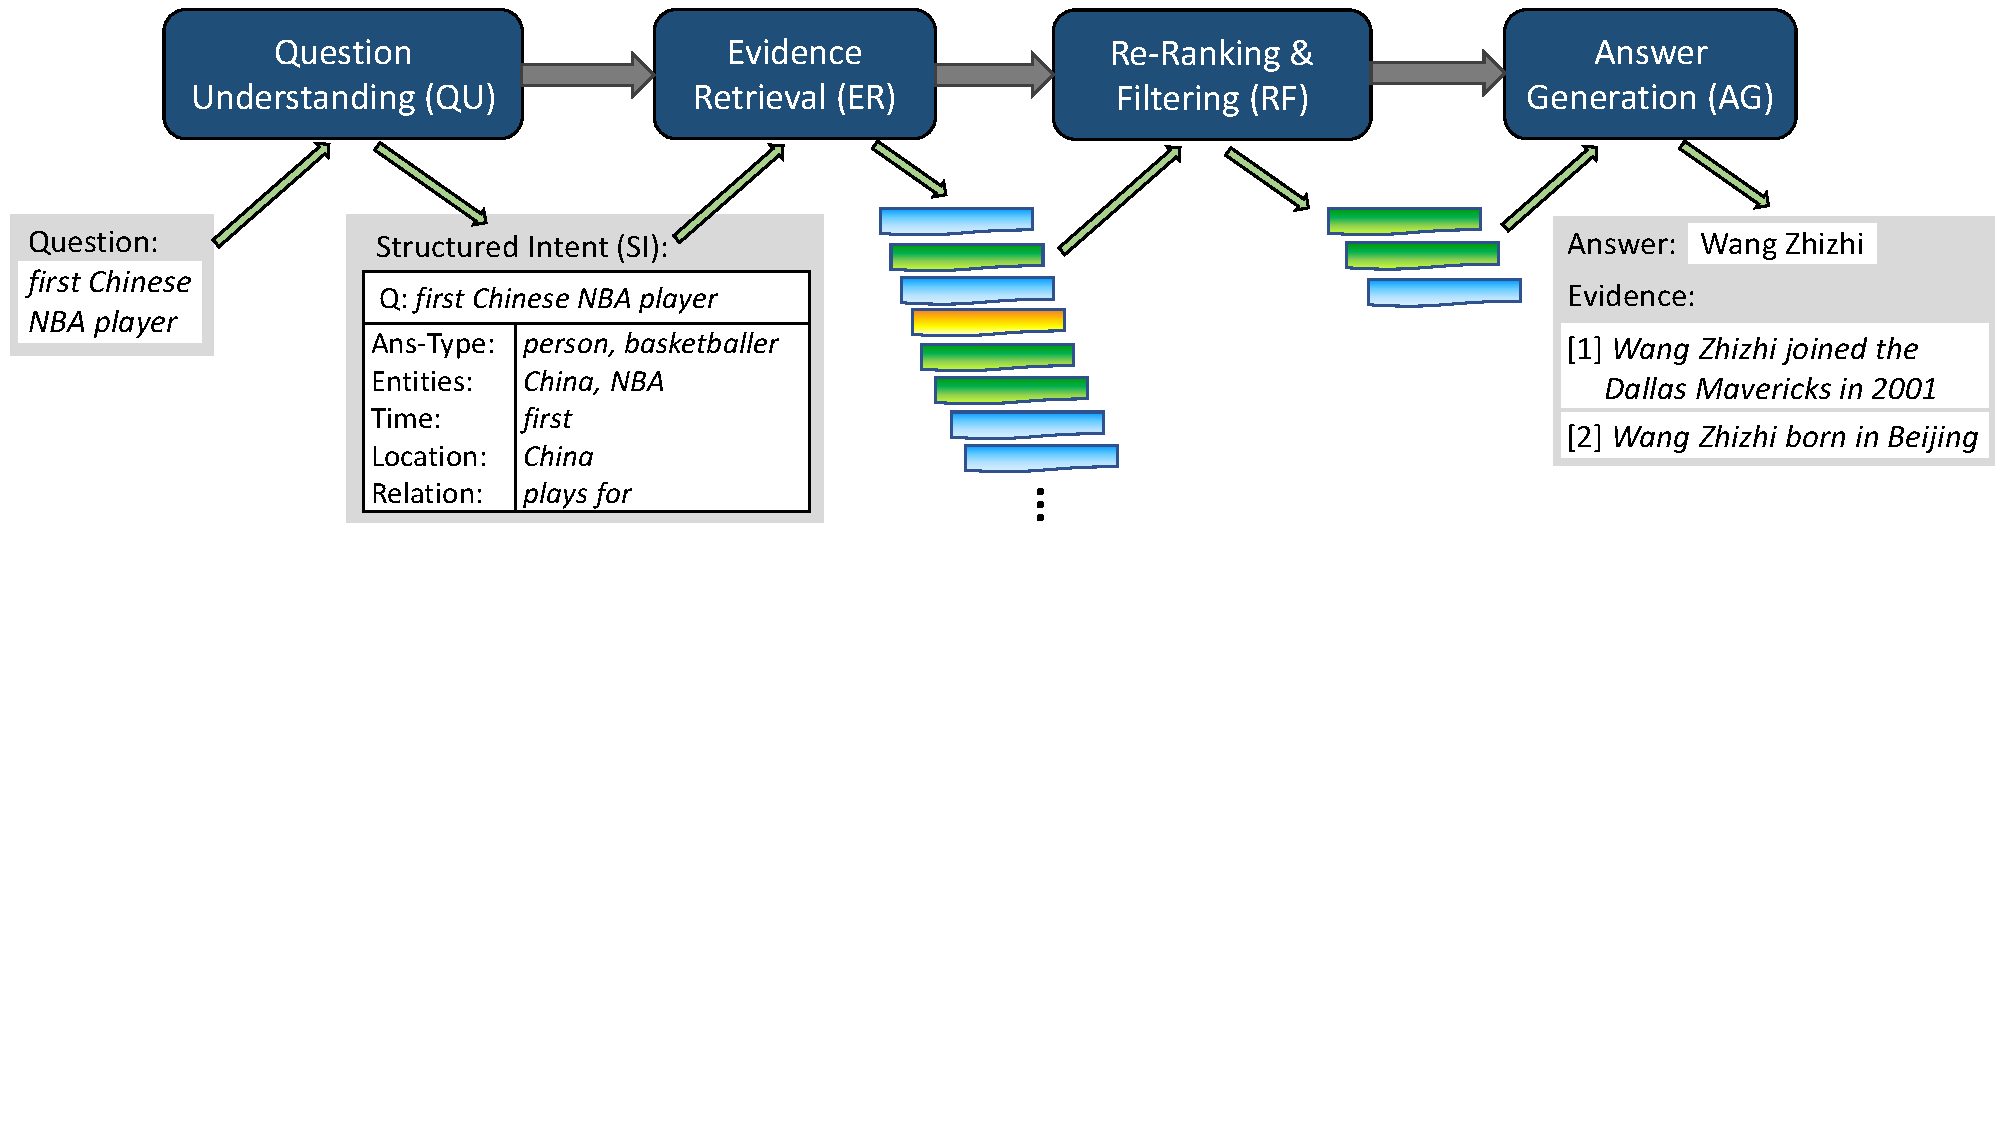
\includegraphics[width=\textwidth]{submissions/Gerhard2024/figures/compass-overview.pdf}
  \caption{Overview of the \method system.}
  \label{fig:compass-overview}
\end{figure}

% start with system overview
The \method system is a pipeline of four major stages, as illustrated in Figure \ref{fig:compass-overview}.
First, the input question is analyzed and decomposed, in order to compute a {\em structured intent (SI)} representation that will pass on to the subsequent steps, along with the original question. Second, the SI is utilized to retrieve pieces of evidence from different sources: text, KG and tables. 
Third, this pool of potentially useful evidence is filtered down, with iterative re-ranking, to arrive at a tractably small set of most promising evidence.
The final stage generates the answer from this evidence,
passing back the answer as well as evidence snippets for user-comprehensible explanation.

The second and fourth stage, Evidence Retrieval (ER) and Answer Generation (AG), are fairly standard. Such a two-phase architecture was called a retriever-reader architecture~\cite{Zhu-ODQA-survey:arxiv2021}. With a modern LLM replacing the earlier kinds of neural readers, this is the core of every RAG system~\cite{DBLP:journals/arXiv/abs-2312-10997}.

Stages 1 and 3 are unique elements of our architecture, judiciously introduced to improve both effectiveness (i.e., answer quality) and efficiency (i.e., computational cost).
Question Understanding (QU) provides the ER component with crisper and semantically refined input, and
the Re-Ranking \& Filtering (RF) stage is beneficial for
distilling the best evidence from the large pool of retrieved pieces.
The following subsections elaborate on the four stages of the pipeline, emphasizing the \method-specific steps QU and RF.



\subsection{Question Understanding (QU)}

% one par introducing the SI
To prepare the retrieval from different kinds of sources, including a KG, ad-hoc tables and text documents, it is useful to analyze and decompose the user question.
In this work, we aim to cast a question into a 
{\em structured intent (SI)} representation: essentially
a frame with faceted cues as slots, or equivalently, a concise set of key-value pairs. 
Figure \ref{fig:compass-overview} gives an idealized example for the question about the first Chinese NBA player. The facets or keys of potential interest here 
are:
\squishlist
\item {\em Ans-Type:} the expected answer type (or types when considering
different levels of semantic refinement), 
\item {\em Entities:} the salient entities in the question, and 
\item {\em Relation:} phrases that indicate which relation (between Q and A entities) the user is interested in. 
\squishend
\noindent In addition, as questions can have temporal or spatial aspects, the SI also foresees slots for:
\squishlist
\item {\em Time:} cues about answer-relevant time points or spans, including relative cues (e.g., ``before Covid'') and ordinal cues (e.g., ``first''), and
\item {\em Location:} cues about answer-relevant geo-locations.
\squishend

% discuss the spectrum of different SIs
\vspace{0.2cm}
\noindent The ideal SI for example question Q2 would look like:

\begin{quote}
{\em Ans-Type:} person, basketballer; {\em Entities:} China, NBA; {\em Time:} first;
{\em Location:} China; {\em Relation:} plays for.
\end{quote}

Note that the values for these slots can be crisp like entity names or dates, but they can also take the form of surface phrases. The SI purpose and value lie in the decomposition. In practice, many questions would only lead to a subset of faceted cues, leaving some slots empty. For the example in Figure \ref{fig:compass-overview}, an alternative SI could simply consist of

\begin{quote}
{\em Ans-Type:} person; {\em Entities:} China, NBA; {\em Time:} first.
\end{quote}

\noindent Even this simplified SI can be highly beneficial in guiding the subsequent evidence retrieval.

% sketch how an LM is trained to generate SIs 
To generate the SI from a user question, we employ a (small-scale) LM, specifically BART~\cite{DBLP:conf/acl/LewisLGGMLSZ20}, a Transformer-based auto-encoder with 140M parameters.\footnote{\url{https://huggingface.co/facebook/bart-base}}
BART is pre-trained for language representation; its power for our purpose comes from fine-tuning.
To this end, we generate (question, SI) pairs by using an instruction-trained LLM like GPT-4, with few-shot in-context learning (following our earlier work~\cite{Jia-FAITH:WWW2024}). 
Note that this is a one-time action; at inference-time we only use much smaller LMs.
The generated silver-standard pairs are then used to fine-tune BART.
In the experiments in this article, we leverage pre-existing collections of silver pairs, based on the training data of the CompMix benchmark~\cite{Christmann-CompMix:WWW2024}, 
comprising $3{,}400$ such pairs.


% outline value of SI for conversations
Although this paper focuses on single-shot questions, the \method architecture is also geared for conversational QA. In that setting, the SI can play an even bigger role, as (follow-up) questions are often formulated in a rather sloppy manner -- all but self-contained. For example, a conversation could start with a clear question {\em When did Wang Zhizhi join the NBA?}, followed a few dialog steps later, by a user utterance like {\em Which teams did he play for?} or simply {\em Which teams?}.
In such an informal conversation, the system needs to {\em contextualize} each user utterance based on the preceding turns in the dialog (e.g., inferring the relevant entities Wang Zhizhi and NBA from the conversational history).
For details on conversational QA, based on our architecture, see our earlier works~\cite{Christmann-CONVINSE:SIGIR2022,Christmann-Explaignn:SIGIR2023}.







%%%%%%%%%%%%%%%%%%%%%%%%%%%%%%%%%%%%%
\subsection{Evidence Retrieval (ER)}

The ER stage taps into a knowledge graph, a corpus of text documents, and a collection of web tables.
Specifically, for the experiments, we use the Wikidata KG,
all English Wikipedia articles, and all tables that are embedded in Wikipedia pages (incl. infoboxes, which can be seen as a special case of tables). 

% specifics: Clocq etc. - and the role of the SI
\vspace{0.2cm}
\noindent{\bf Retrieval from KG:}
To retrieve evidence from the KG, we utilize our earlier work
\clocq~\cite{Christmann-CLOCQ:WSDM2022}, which provides entity disambiguations and a relevant KG-subgraph for a given query.
Unlike most other works on QA-over-KG, \clocq fetches all KG-facts that are relevant for a given entity in a single step.
For example, when querying for
NBA players, it can traverse the KG neighborhood and pick up top teams, also considering so-called qualifier nodes in Wikidata which are often used for temporal scopes. 
As the disambiguation of entity names onto the KG can be tricky and noisy (e.g., China could be mapped to Chinese sports teams in all kinds of sports), \clocq considers several possible disambiguations~\cite{Christmann-CLOCQ:WSDM2022} (typically in the order of $10$ result entities).
The queries for \clocq are 
constructed by concatenating all slots of the question's SI.
For the example query about the first Chinese NBA player,
good result entities would be Dallas Mavericks, lists about NBA seasons, MVP awards etc., and their associated facts. These provide cues, but are likely insufficient to answer the question.


\vspace{0.2cm}
\noindent{\bf Retrieval from Text and Tables:}
The disambiguated entities returned by \clocq form anchors for tapping into text and tables.
\method first identifies 
relevant text documents and tables that refer to the anchor entities. With focus on Wikipedia, these are simply the articles for the respective entities. 
\method then constructs a keyword query that concatenates all available fields of the SI.
The query is evaluated against a linearized and verbalized representation (see below) of all sentences and all table rows in the selected documents.
This returns a set of sentences and 
and individual table rows, ranked by BM25 scores.


\vspace{0.2cm}
\noindent{\bf Evidence Verbalization:}
All results from the different data sources are uniformly treated by {\em linearizing} and {\em verbalizing} them
into token sequences. For KG results, the entity-centric triple sets are linearized via breadth-first traversal of the mini-graph starting from the entity node.
For tables, results are individual rows, which are contextualized by including labels from column headers and from the DOM-tree path of the article where the table comes from. For example, a table row about Wang Zhizhi playing for Dallas (Mavericks) in the 2000-2001 season, would be expressed as:

\vspace{0.05cm}
\hspace*{0.5cm} Wang Zhizhi / NBA Career / Season: 2000-2001, Team: Dallas, Games Played: 5 \dots
\vspace{0.05cm}

\noindent Finally, results from the text corpus are already in the form of token sequences, but we can additionally prefix these with the DOM-tree labels.
We can think of this entire pool of evidence as 
an on-the-fly corpus of potentially relevant pseudo-sentences, forming the input of the subsequent RF stage.


\vspace{0.2cm}
\noindent {\bf Result Ranking:}
Overall, the ER stage compiles a substantial set of evidence, possibly many thousands of entities, text snippets and table rows. Therefore, we practically restrict the pool to a subset of high-scoring pieces, like the top-$1000$.
For scoring, a simple BM25 model (a classical IR method) is applied. 
By default, we treat all evidence pieces uniformly with global scoring, no matter whether they come from KG, text or tables. 


\subsection{Re-Ranking and Filtering (RF)}

With a pool of top-$1000$ evidence pieces, we could invoke an LLM for answer generation. However, that would face a large fraction of noise (i.e., misleading evidence) and incur high costs of computation and energy consumption. 

For both of these reasons, we have devised light-weight techniques for iteratively reducing the top-$1000$ pieces to a small subset, say top-$30$ or top-$10$, that can be fed into an LLM at much lower cost (as LLM computations and pricing are at least linear in the number of input tokens). The difficulty is, of course, to do this without losing good evidence and reducing answer presence. Our techniques for this task are based on graph neural networks (GNNs)~\cite{Wu:IEEE2021} or cross-encoders (CEs)~\cite{Dejean:arxiv2024,Lin:MC2021}.

\myparagraph{GNN-based RF}
Given a large pool of evidence pieces from all sources, a bipartite graph is constructed:
\squishlist
\item {\em nodes} being evidence pieces or entities that occur in these pieces, and
\item {\em edges} connecting an evidence piece and an entity if the entity occurs in the evidence.
\squishend


The task for the GNN is to jointly score the evidence and the entity nodes in a multi-task learning setup. The latter are the {\em answer candidates}, and the evidence should give {\em faithful explanation} for an answer.
We build on our earlier work on explainable QA~\cite{Christmann-Explaignn:SIGIR2023}.

The node encodings are initialized with cross-encoder embeddings (see below) 
for node contents and the SI of the question. The inference iteratively adjusts the encodings based on message passing from neighboring nodes.
The GNN is trained via weak supervision from question-answer pairs:
evidence nodes are labeled as relevant if they are connected to
a gold answer.
More technical details are given in~\cite{Christmann-Explaignn:SIGIR2023}.

\method invokes the GNN in multiple rounds, iteratively reducing top-$k$ to top-$k^*$ nodes with $k^* \ll k$. In practice, we would typically consider two rounds: re-ranking top-$1000$ and pruning to top-100, and then reducing to top-30 or top-10, which are passed to the answer generation stage.
Note that this keeps the GNN at a tightly controlled size, so that its computational costs at inference-time are much smaller than those of an LLM.


\myparagraph{CE-based RF}
An alternative to the GNN inference is to employ a cross-encoder for scoring and re-ranking the evidence pieces.
These are transformers (typically with a small LM like BERT) that are fine-tuned for scoring the relatedness between a query and a document~\cite{Nogueira:arxiv2019}. In our case, the comparison is between the question SI and the evidence piece. In our experiments, we make use of two different cross-encoders, 
both trained on the MS-MARCO benchmark for passage retrieval~\cite{Bajaj:arxiv2018}, 
and fine-tuned on the respective benchmark (leveraging the same weak supervision data as for the GNNs),
the difference being in model size.\footnote{\url{https://huggingface.co/cross-encoder/ms-marco-MiniLM-L-4-v2} and\\ \url{https://huggingface.co/cross-encoder/ms-marco-MiniLM-L-6-v2}}
We use the smaller model to reduce top-$1000$ to top-100, and the larger model to go further down from top-100 to top-30.




%%%%%%%%%%%%%%%%%%%%%%%%%%%%%%%%%%%%%

\subsection{Answer Generation (AG)}

The last stage follows mainstream practice to invoke an LLM in a retrieval-augmented manner.
We call a `small-scale` LLM, specifically a fine-tuned LlaMA-3.1 model (8B-Instruct)\footnote{\url{https://huggingface.co/meta-llama/Llama-3.1-8B-Instruct}}, with a prompt \footnote{The specific prompt is \phrase{SI: \textless\texttt{concatenated SI}\textgreater \hspace{0.1cm} Evidence: \textless\texttt{evidence pieces}\textgreater}.}
consisting of:

\squishlist
\item the concatenated SI of the original question, and
\item the top-30 (or other top-$k^*$ with small $k^*$) evidence pieces.
\squishend

By the previous down-filtering of the original pool of evidence pieces, this last step has affordable cost in terms of computation time and energy consumption.

\vspace{0.2cm}
\noindent{\bf Fine-Tuning the LLM:}
We considered adding an instruction to the prompting, such as {\em ``answer this question solely based on the provided evidence snippets''}.
However, this turned out to be ineffective.
The reason why the model works well without such instructions is our task-specific fine-tuning.
We perform this by running the training data of benchmarks through the \method pipeline,
and training the AG stage with the top-30 evidence pieces as input.
Thus, the fine-tuning makes the model learn the role of evidence for RAG-based QA.

\vspace{0.2cm}
\noindent{\bf Explanations:}
The top-30 evidence pieces can be used to provide users with explanation of answers.
Optionally, these could be reduced further for comprehensibility.
Alternatively, we can fine-tune the LLM to provide both answers and concise explanations.
Since we can infer which evidences in the input mention the annotated ground-truth answers,
our method could be fine-tuned to provide such \textit{answering evidences} as well (cf.~\cite{Gao-citations:emnlp2023}).

\label{sec:exp}
\section{Experiments}


\label{setup}
\subsection{Experimental setup}


%%% BENCHMARKS
\myparagraphnospace{Benchmarks} We run experiments on three benchmarks with different characteristics of questions.

\squishlist
    \item \textbf{\compmix}.
    \compmix~\cite{Christmann-CompMix:WWW2024} is a benchmark which was specifically designed for evaluating QA systems operating over heterogeneous sources. The dataset has $9{,}410$ questions, out of which $2{,}764$ are used for testing.
    Answers are crisp entity names, dates, or other literals.
    
    \item \textbf{\crag}.
    We further evaluate on a subset of the \crag~\cite{Yang-CRAG} dataset, which was recently released as a testbed for RAG-based QA systems.
    We utilize the same pipeline and sources as outlined in Section~\ref{sec:method}, without using the web snippets or APIs provided with \crag. This way we focus on entity-centric questions that do not require access to live web data (e.g., news feeds), and disregard cases where the results would be up-to-date quantities.
    This restricts the test data to $436$ entity-centric questions, still enough for a proof of concept.
    
    \item \textbf{\timequestions}.
    To showcase the generalizability of our pipeline, we conduct experiments on~\timequestions~\cite{Jia-TimeQuestions},
    a benchmark for temporal QA. The dataset requires temporal understanding and reasoning, which are well-known limitations of
    LLMs~\cite{Dhingra-time-aware-LLM:TACL2022}. \timequestions has 16{,}181 questions (3{,}237 for testing).
\squishend

Typical examples for the questions in these three benchmarks are:

\begin{quote}
\compmix: \utterance{Which player won the most number of Man-of-the-Match titles in the FIFA world cup of 2006?}\\
 \indent \crag: \utterance{What was the worldwide box office sales for little hercules?}\\ 
  \indent \timequestions: \utterance{Which club did Cristiano Ronaldo play for before joining Real Madrid?}
\end{quote}

%%% BASELINES
\myparagraph{Baselines} As competitors or reference points to \method, we study the performance of the following methods:

\squishlist
    \item \textbf{Generative LLMs}.
    We compare \method against out-of-the-box LLMs: \textbf{\gptthree} (\texttt{text-davinci-003}), \textbf{\gptfour} (\texttt{gpt-4}) 
    and \textbf{\llama} (\texttt{meta-llama/Llama-3.1-8B-Instruct}).
    The same prompt is used for all LLMs, consistent with previous work~\cite{Christmann-CompMix:WWW2024, Zhang-Spaghetti:ACL2024}:
    \phrase{Please answer the following question by providing the crisp answer entity, date, year, or numeric number. Q: \textless\texttt{question}\textgreater}.
    

    \item \textbf{Heterogeneous QA methods}.
    \convinse~\cite{Christmann-CONVINSE:SIGIR2022}, \unikqa~\cite{Oguz-UniK-QA:NAACL2022}, \explaignn~\cite{Christmann-Explaignn:SIGIR2023}
    are QA methods designed to integrate heterogeneous sources: text, tables and KG. All of these  integrate the exact same sources as \method.

    
    \item \textbf{\textsc{State-of-the-art}}.
    For \compmix and \timequestions, we also compare against state-of-the-art methods from the literature: \spaghetti~\cite{Zhang-Spaghetti:ACL2024} and \textsc{Un-Faith}~\cite{Jia-FAITH:WWW2024}, which are among the best performing systems.
    
Results are taken from the literature whenever applicable.
On \crag, we use the models trained on \compmix for \method and heterogeneous QA baselines.
\squishend



%%% METRIC(S)
\myparagraph{Metrics}
We measure \textit{precision at 1} (\textbf{P@1}) as our main metric~\cite{RoyAnand:MC2021} on all benchmarks.
On \crag, we manually annotate answer correctness, as the ground-truth answer formats vary (e.g., entity name variants, lists, sentences).

We also compute the number of neural parameters aggregated over all sub-modules (\textbf{\#Parameters}).
Parameter counts for GPT-models are taken from~\cite{Minaee-LLM-survey}
(\gptfour might have less active parameters during inference).

For further analysis we measure \textit{answer presence} (\textbf{AP@k}),
i.e. whether the answer is present in the top-$k$ ranked evidence pieces,
and \textit{mean reciprocal rank} within the top-$k$ evidences (\textbf{MRR@k}).

%%% CONFIG
\myparagraph{Configuration}
Our implementation uses the \texttt{Llama3.1-8B-Instruct} model for the AG stage.
For the QU, ER and RF stages
we adopt code from the \explaignn project.\footnote{\url{https://explaignn.mpi-inf.mpg.de}}
For the ER stage, we use \clocq, setting its specific parameters to $k=10$ and $p=1{,}000$.

As default, we use the GNN technique for the RF stage.
For efficiency, we use light-weight models for initializing
the GNN encoders -- the same models used for the CE-based RF.\footnote{\url{https://huggingface.co/cross-encoder/ms-marco-MiniLM-L-4-v2} and\\\url{https://huggingface.co/cross-encoder/ms-marco-MiniLM-L-6-v2}}
The GNNs are trained for $5$ epochs with an epoch-wise evaluation strategy,
i.e. we choose the model with the best performance on the respective dev set.
We train the GNNs on graphs with a maximum of $100$ evidence and $400$ entity nodes (as scored by BM25).
During inference, the first GNN is applied on graphs with $1{,}000$ evidence and $4{,}000$ entity nodes, shrinking the pool of evidence pieces to the top-$100$.
The second GNN then runs on graphs with $100$ evidence and $400$ entity nodes.
The factor of 4 entities per evidence (on average) holds sufficient for the observed data,
and enables batched inference.
Other parameters are kept as is.

The AG model, based on \texttt{Llama3.1-8B-Instruct}, is 
fine-tuned
for $2$ epochs with a warm-up ratio of $0.01$ and a batch size of $8$, again with an epoch-wise evaluation strategy.
Other parameters are set to the default Hugging Face
training parameters.\footnote{\url{https://huggingface.co/docs/transformers/v4.46.2/en/main_classes/trainer\#transformers.TrainingArguments}}





\subsection{Main results}
%%% MAIN TABLE
\myparagraphnospace{\method is competitive on all benchmarks}
Main results of our experiments are shown in Table~\ref{tab:main-res}.
First of all, we note that \method achieves competitive performance across all three benchmarks.

On \compmix, baselines for heterogeneous QA and \llama perform similarly,
whereas GPT-based LLMs can answer more than $50$\% of the questions correctly.
\method exhibits substantially higher performance, on par with
the state-of-the-art method \textsc{Spaghetti}~\cite{Zhang-Spaghetti:ACL2024}
(which is based on \gptfour).

On the \crag dataset, P@1 drops for all methods except for \gptfour. 
The benchmark includes realistic questions,
which can be ambiguous/confusing (\phrase{who was the director for the report?}),
on ``exotic'' entities with answers in social media (\phrase{how many members does the teknoist have?}),
or require up-to-date information (\phrase{when did chris brown release a song or album the last time?}),
and other cases that are challenging for all methods.

Finally, \method establishes new state-of-the-art performance on the \timequestions benchmark.
Interestingly, all of the tested LLMs show greatly reduced performance on this benchmark,
which inherently requires temporal understanding and reasoning
-- a known weakness of stand-alone LLMs.


\begin{table} [h]
    \centering
    \newcolumntype{G}{>{\columncolor [gray] {0.90}}c}
    \begin{tabular}{l G G G c}
        \toprule
            \textbf{Method $\downarrow$ / Benchmark $\rightarrow$} & \textbf{\compmix}  & \textbf{\crag} & \textbf{\timequestions} & \textbf{\#Parameters} \\ 
        \midrule
            \textbf{\gptthree} 
            & $0.502$ &   $-$ & $0.224$ & $175{,}000$ M  \\
            % #params from https://arxiv.org/pdf/2402.06196

            \textbf{\gptfour}
            & $0.528$ &   $\mathbf{0.633}$ & $0.306$ & $1{,}760{,}000$ M \\
            % #params from https://arxiv.org/pdf/2402.06196

            \textbf{\llama~\cite{Touvron-LLaMA}} (8B-Instruct)
            & $0.431$ &   $0.385$ & $0.178$ & $8{,}030$ M  \\
            % #params from Huggingface (8,030,257,152)
        \midrule
            \textbf{\convinse~\cite{Christmann-CONVINSE:SIGIR2022}}
            & $0.407$  &   $0.298$ & $0.423$  & $362$ M \\
            % FiD: 222,903,936 + BART (SR-generation): 139,420,416 = 362,324,352 (python explaignn/question_understanding/structured_representation/get_num_params.py)

            \textbf{\unikqa~\cite{Oguz-UniK-QA:NAACL2022}}
            & $0.440$ &   $0.280$ & $0.424$ & $223$ M  \\
            % FiD: 222,903,936 (python explaignn/heterogeneous_answering/fid_module/FiD/get_num_params.py)
    
            \textbf{\explaignn~\cite{Christmann-Explaignn:SIGIR2023}} 
            & $0.442$ &   $0.303$ & $0.525$  & $328$ M \\
            % BART (SR-generation): 139,420,416 + 2GNNs: 94520832 + 93930240 = 327,871,488

        \midrule 
            \textbf{\textsc{State-of-the-art}}
            & $\mathbf{0.565}$ 
            & $-$
            & $0.571$  & $-$ \\

            & (\textsc{Spaghetti}~\cite{Zhang-Spaghetti:ACL2024})
            & 
            & (\textsc{Un-Faith}~\cite{Jia-FAITH:WWW2024}) &  \\

        \midrule
            \textbf{\method (ours)}
            & ${0.564}$ &   $0.362$ & $\mathbf{0.754}$  & $8{,}218$ M \\
            % BART (SR-generation): 139,420,416 + LLaMA: 8,030,257,152 + GNNs: 25,670,016 + 22,268,928 =  8,217,616,510
        \bottomrule
    \end{tabular} 
    \vspace*{-0.2cm}
    \caption{End-to-end P@1 of \method and baselines on three benchmarks. Results for \gptthree and \gptfour are taken from the literature~\cite{Christmann-CompMix:WWW2024, Jia-FAITH:WWW2024}. \gptthree is not accessible anymore, hence no results on \crag.
    }
    \label{tab:main-res}
\end{table}





%%% ANSWER SOURCES
\myparagraph{Integration of heterogeneous sources is vital}
\method integrates evidence from text, KG and tables into a unified framework.
We aim to better understand how this affects the answering performance of the method.
Table~\ref{tab:sources} shows end-to-end answering performance of \method
with different combinations of the input sources.
The results clearly indicate that all types of sources contribute, with option Text+KG+Tables performing best,
with a large margin over tapping only single source types.

\begin{table} [t] 
    \centering
    \newcolumntype{G}{>{\columncolor [gray] {0.90}}c}
    \newcolumntype{H}{>{\setbox0=\hbox\bgroup}c<{\egroup}@{}}
    	\begin{tabular}{l G G G H H H c c c} 
        \toprule
            \textbf{Benchmark $\rightarrow$}
                & \multicolumn{3}{G}{\textbf{\compmix}} 
                & \multicolumn{3}{H}{\textbf{\crag}}
                & \multicolumn{3}{c}{\textbf{\timequestions}} \\ 
        \midrule
            \textbf{Input sources $\downarrow$ / Metric $\rightarrow$}
                & \textbf{P@1} & \textbf{AP@100}  & \textbf{AP@30}
                & \textbf{P@1} & \textbf{AP@100}  & \textbf{AP@30}
                & \textbf{P@1} & \textbf{AP@100}  & \textbf{AP@30} \\
            \midrule
                \textbf{Text}           &  $0.455$  &  $0.563$  &  $0.531$ &  $?$  &  $?$  &  $?$ &  $0.539$  &  $0.515$  &  $0.487$   \\
                \textbf{KG}             &  $0.481$  &  $0.677$  &  $0.637$ &  $?$  &  $?$  &  $?$ &  $0.724$  &  $0.701$  &  $0.674$   \\
                \textbf{Tables}         &  $0.432$  &  $0.501$  &  $0.482$ &  $?$  &  $?$  &  $?$ &  $0.536$  &  $0.347$  &  $0.328$   \\
            \midrule
                \textbf{Text+KG}        &  $0.537$  &  $0.749$  &  $0.706$ &  $?$  &  $?$  &  $?$ &  $0.745$  &  $\mathbf{0.776}$  &  $0.748$   \\
                \textbf{Text+Tables}    &  $0.503$  &  $0.632$  &  $0.594$ &  $?$  &  $?$  &  $?$ &  $0.567$  &  $0.578$  &  $0.549$   \\
                \textbf{KG+Tables}      &  $0.524$  &  $0.728$  &  $0.692$ &  $?$  &  $?$  &  $?$ &  $ 0.743$  &  $0.731$  &  $0.703$   \\
            \midrule
                \textbf{Text+KG+Tables}    &  $\mathbf{0.564}$  &  $\mathbf{0.759}$  &  $\mathbf{0.724}$ &  $?$ &  $?$  &  $?$ & $\mathbf{0.754}$    & $\mathbf{0.776}$  &  $\mathbf{0.749}$   \\
            \bottomrule
    \end{tabular}
    \vspace*{-0.2cm}
    \caption{Answer presence and answering precision of \method with different combinations of input sources (on the respective test sets).}
    \label{tab:sources}
\end{table}




\subsection{Analysis}

%%% TOP-K vs. 3xTOP-(K/3)
\myparagraph{Unified retrieval enhances performance}
In the RF stage, we re-rank and filter evidence from different source types,
and feed the unified top-\textit{k}* into the AG stage.
We conduct a comparison in which we consider
the top-$10$ evidence pieces from each source type individually. This gives equal influence to KG, text and tables, whereas our default is based on global ranking.
Table~\ref{tab:unified-retrieval} shows the results for this analysis, showing our default choice performs better.
The reason is that different questions require different amounts of evidence from each of the source types.

\begin{table} [t] 
    \centering
    \newcolumntype{G}{>{\columncolor [gray] {0.90}}c}
    \newcolumntype{H}{>{\setbox0=\hbox\bgroup}c<{\egroup}@{}}
    	\begin{tabular}{l G G H H} 
        \toprule
            \textbf{Input evidences $\downarrow$ / Metric $\rightarrow$} & \textbf{P@1} & \textbf{AP@30}  & \textbf{\crag} & \textbf{\timequestions} \\ 
            \midrule
                \textbf{Top-30 Text+KG+Tables (ours)}             &  $\mathbf{0.574}$  &  $\mathbf{0.710}$  &  $-$  &  $-$   \\
                \textbf{Top-10 Text + Top-10 KG + Top-10 Tables}        &  $0.560$    &  $0.709$  &  $-$  &  $-$   \\
            \bottomrule
    \end{tabular}
    \vspace*{-0.2cm}
    \caption{Answer presence and precision
    of \method for different choices of top-30 
    (on \compmix dev set).}
    \label{tab:unified-retrieval}
\end{table}


%%% NUMBER OF EVIDENCES
\myparagraph{\method works well with small amounts of evidence}
We investigate the 
influence of 
the number of evidence pieces
fed into the AG stage, varying it from $5$ to $100$.
Results are shown in Figure~\ref{fig:res-num-evidences}.
As the curve shows, there is a sharp increase in precision as we add evidence up to 30 or 40 pieces, which is around our default of top-30. This indicates that a certain amount of evidence is needed, to overcome the inherent noise and arrive at sufficient answer presence. 
As we increase the amount of evidence further, we observe a saturation effect, and eventually a degration of performance. Too much evidence not only has diminishing returns, but can actually be confusing for the AG stage. This reconfirms our heuristic choice of top-30: enough for good answering while keeping computational costs reasonably low.


\begin{figure}[t]
    \centering
    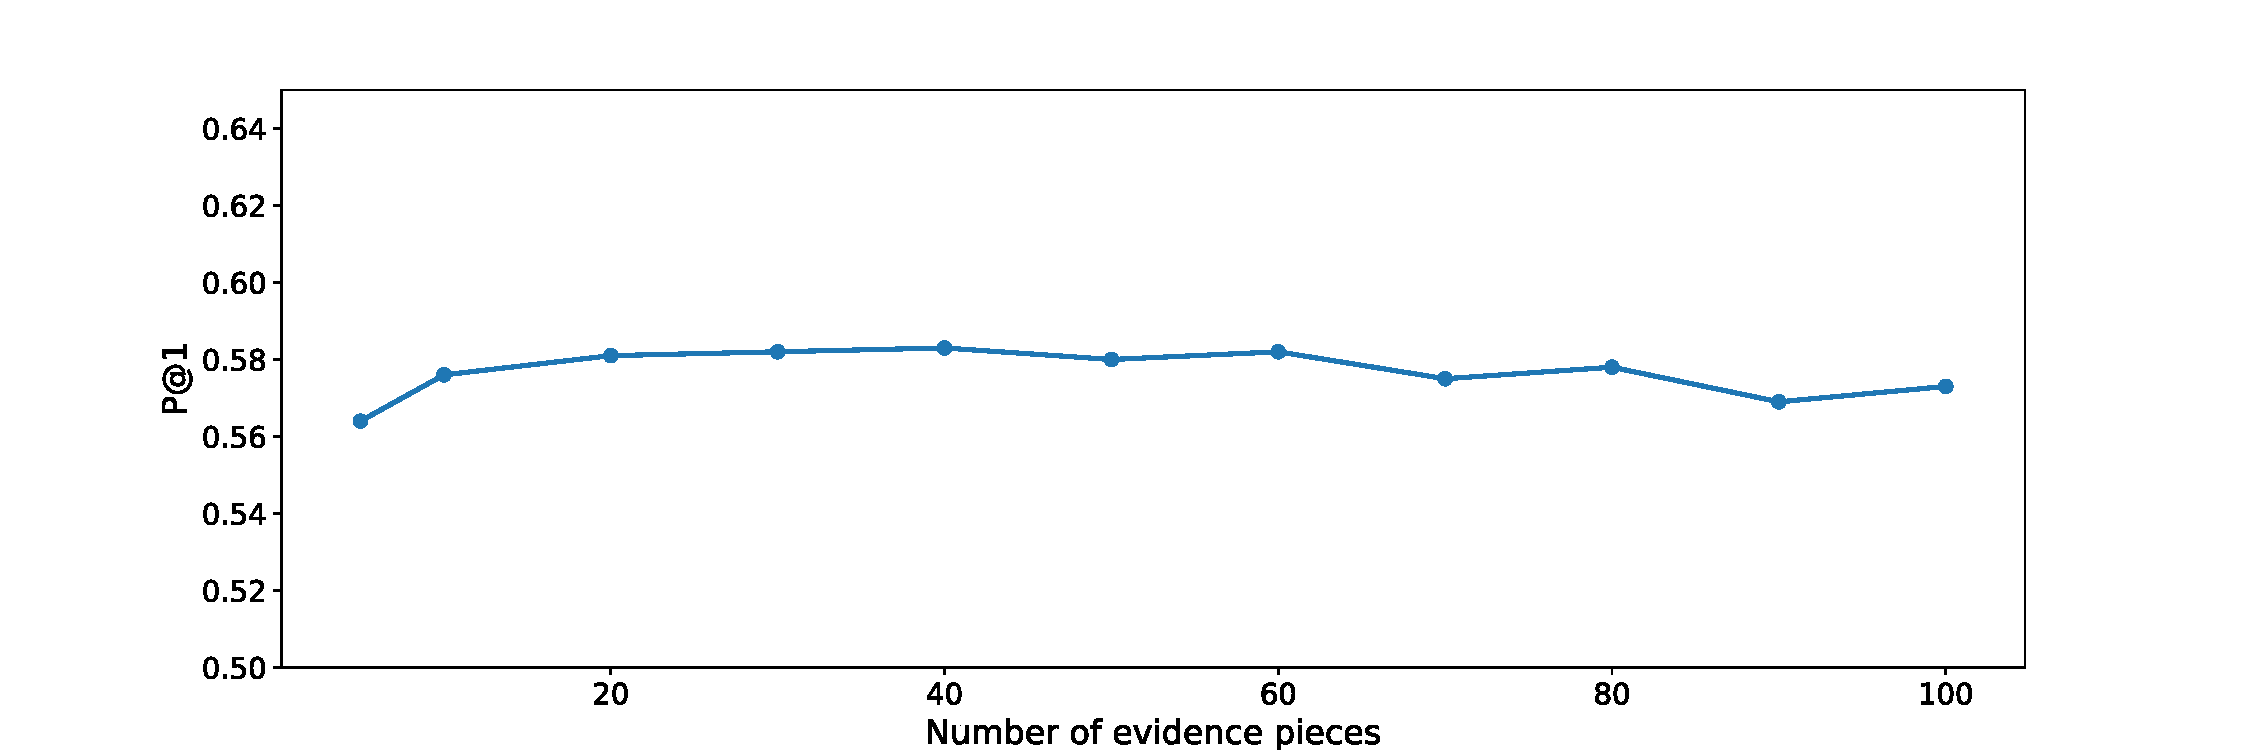
\includegraphics[width=0.8\textwidth]{submissions/Gerhard2024/figures/p_at_1-line_with_evidences.pdf}
    \vspace*{-0.2cm}
    \caption{Performance of \method on the \compmix dev set with different numbers of evidence.}
    \label{fig:res-num-evidences}
    \vspace*{-0.2cm}
\end{figure}



%%% ABLATION
\myparagraph{Ablation study on re-ranking} For more insight on the possible configurations of the RF stage, we conducted an ablation study with different options, including solely relying on the initial BM25 scoring without explicit re-ranking. The results are shown in Table \ref{tab:ablation2}. We observe that the iterative reduction in two steps is slightly better than the single-step variants (going down from top-1000 to top-30 in one RF step). Between the two options of using a GNN or a CE, the differences are negligible. A notable effect is that our RF techniques retain the answer presence at a very high level, only a bit lower than for the initial top-1000. 
The last two rows of Table \ref{tab:ablation2} demonstrate that RF is crucial: without explicit re-ranking, the technique of just picking smaller top-$k$ from the original BM25 model leads to substantial degradation in both answer presence and precision. 


\begin{table} [t] \small
    \centering
    \newcolumntype{G}{>{\columncolor [gray] {0.90}}c}
    \newcolumntype{H}{>{\setbox0=\hbox\bgroup}c<{\egroup}@{}}
    	\begin{tabular}{l G H G G G} 
        \toprule
            & \multicolumn{5}{G}{\textbf{\compmix} (dev set)} \\
        \midrule
            \textbf{RF Method $\downarrow$ / Metric $\rightarrow$} & \textbf{P@1} & \textbf{AP@1000} & \textbf{AP@100}  & \textbf{AP@30} & \textbf{MRR@100} \\ 
        \midrule
            \textbf{GNN: 1000 $\rightarrow$ 100 $\rightarrow$ 30}             &  $\mathbf{0.574}$  & $0.760$ &  $0.738$  &  $0.710$  &  $\mathbf{0.572}$  \\
            \textbf{CE: 1000 $\rightarrow$ 100 $\rightarrow$ 30}          &  $0.573$  & $0.760$  &   $\mathbf{0.740}$ &  $\mathbf{0.721}$   &  $0.553$   \\
        \midrule
            \textbf{GNN: 1000 $\rightarrow$ 30} &  $0.567$  & $?$  &   $n/a$ &  $0.710$   &  $0.567$   \\
         \textbf{CE: 1000 $\rightarrow$ 30} &  $0.570$  & $0.760$  &   $n/a$ &  $0.715$   &  $0.558$   \\
            \midrule
           \textbf{BM25: 100 (w/o GNN or CE)} &  $0.490$ & $0.760$  &  $0.652$  &  $n/a$  &  $0.259$ \\       
            \textbf{BM25: 30 (w/o GNN or CE)} &  $0.468$  & $0.760$  &  $n/a$ &  $0.534$   &  $0.259$   \\
            \bottomrule
    \end{tabular}
    \vspace*{-0.2cm}
    \caption{Ablation study for different RF strategies of \method on the \compmix dev set. The answer presence in the RF input with top-$1000$ evidence pieces is $0.760$.}
    \label{tab:ablation2}
\end{table}



\myparagraph{Quality of SI}
To assess the quality and robustness of the Structured Intents, we
inspected a sample of questions and their SIs.
Table~\ref{tab:question-SI-examples} gives three anecdotic examples.
We show SIs generated by \method, which makes use of the pre-existing collection from the \compmix benchmark for training.
This training data was obtained via different heuristics, 
which can be a limiting factor when user intents become more complex.

Therefore, we also looked at SIs derived via in-context learning (ICL) using \gptfour with $5$ handcrafted examples.
As shown in our earlier work on temporal QA~\cite{Jia-FAITH:WWW2024},
such data can be used for training smaller models (e.g., BART),
which can greatly boost the completeness and overall quality of the generated SIs.

From the sampled set, we observed that the ICL-based SIs are more
complete with all slots filled, whereas the BART-based SIs focused more
on the main slots Answer-type, Entities and Relation.
However, both approaches achieve very high quality in filling the slots,
capturing the user's information need very well.

Interestingly, when questions get complicated, with nested phrases, 
the ICL-based variant succeeds in decomposing the questions, based on only $5$ ICL examples.
For example, for the question {\em ``which German state had the most Corona-related death cases in the first year after the outbreak?''}
the Time slot becomes {\em ``first year after Corona outbreak''},
which can be resolved to identify the temporal scope.
In general, we believe that such question decomposition, beyond simple temporal constraints,
would be an interesting theme for future work.

\begin{table} [t] 
    \centering
    \small
    \newcolumntype{G}{>{\columncolor [gray] {0.90}}c}
    \newcolumntype{H}{>{\setbox0=\hbox\bgroup}c<{\egroup}@{}}
    \resizebox*{\textwidth}{!}{
        \begin{tabular}{p{6cm}|p{6cm}|p{6cm}} 
        \toprule
            \textbf{Question} & \textbf{Current SI by \method} & \textbf{SI via ICL} \\
        \midrule
        \textit{what was disneys first color movie?}
            & Ans-Type: \textit{animated feature film} & Ans-Type: \textit{film, animated film} \\
            & Entities: \textit{disneys} & Entities: \textit{Disney} \\
            & Relation: \textit{was first color movie} & Relation: \textit{first color movie} \\
            &  & Time: \textit{first} \\
        \midrule
        \textit{at the oscars, who won best actor in 2018?}
            & Ans-Type: \textit{human} & Ans-Type: \textit{person, actor} \\
            & Entities: \textit{at the oscars} & Entities: \textit{Oscars, 2018} \\
            & Relation: \textit{who won best actor in 2018} & Relation: \textit{won best actor} \\
            &  & Time: \textit{2018} \\
        \midrule
        \textit{which German state had the most Corona-} & Ans-Type: \textit{state} & Ans-Type: \textit{location, state} \\
        \textit{related death cases in the first year after} & Entities: \textit{Germany, Corona} & Entities: \textit{Germany, Corona-related deaths} \\
        \textit{the outbreak?} & Relation: \textit{which state had the most related} & Relation: \textit{highest count of death cases} \\
        & \textit{death cases in the first year after the out-}  & Location: \textit{Germany} \\
            & \textit{break}  & Time: \textit{first year after Corona outbreak} \\
        \bottomrule
    \end{tabular}
    }
    \vspace*{-0.2cm}
    \caption{Examples for pairs of question and generated SI.}
    \label{tab:question-SI-examples}
\end{table}




%%% REFRAIN FROM ANSWER
\myparagraph{Refraining from answering}
%%% Searched for: "generated_answer I" (with I being the full word, not partial) in the generated answers of LLaMA
%%% yields 245 results out of 2764 questions on CompMix
%%% yields 1270 results out of 3237 questions on TimeQuestions
We can train our model to refrain from answering in scenarios
where the provided evidence does not contain an answer to the question.
Specifically, during training, when the answer is not present in the evidence,
we change the target answer to {\em unknown}. This variant is referred to as \method {\em (faithful)}.

We measure the ratio of questions for which {\em unknown} is provided as answer,
and the P@1 restricted to questions that are answered.
The accuracy of refraining from answering is measured as well,
based on whether the answer is present in the evidence or not.
We conduct this experiment on \compmix and \timequestions,
for which we can compute answer presence exactly.
We also compute results for \llama, which is already instructed 
with the option to answer ``don't know''.
Table~\ref{tab:refrain-from-answer} shows the results.
For \compmix, we observe that \method has high accuracy on refraining when appropriate,
whereas \llama tends to be overconfident with a very small rate of {\em unknowns}, leading to incorrect answers.

\begin{table} [t] \small
    \centering
    \newcolumntype{G}{>{\columncolor [gray] {0.90}}c}
    \newcolumntype{H}{>{\setbox0=\hbox\bgroup}c<{\egroup}@{}}
    	\begin{tabular}{l G G G G c c c c} 
        \toprule
            & \multicolumn{4}{G}{\textbf{\compmix}} & \multicolumn{4}{c}{\textbf{\timequestions}} \\
            \midrule
            \textbf{Metric $\rightarrow$} & \textbf{P@1}  & \textbf{P@1} & \textbf{Refrain} & \textbf{Refrain} & \textbf{P@1}  & \textbf{P@1} & \textbf{Refrain} & \textbf{Refrain} \\ 
            \textbf{Method $\downarrow$} &                 & \textbf{(answered)} & \textbf{rate} & \textbf{accuracy} &                 & \textbf{(answered)} & \textbf{rate} & \textbf{accuracy} \\ 
            \midrule
                \textbf{\llama}             &  $0.431$  &  $0.471$  &  $0.089$  &  $n/a$  &  $0.177$  &  $0.276$  &  $0.392$  &  $n/a$  \\
                \textbf{\method (faithful)}           &  $0.497$  &  $0.713$  &  $0.303$  &  $0.838$ &  $0.597$  &  $0.804$  &  $0.257$  &  $0.864$  \\
            \bottomrule
    \end{tabular}
    \vspace*{-0.2cm}
    \caption{
        Performance of \method with option to refrain from answering (``don't know'').
    }
    \label{tab:refrain-from-answer}
\end{table}

\label{sec:disc}
\section{Insights, Limitations, and Challenges}


\noindent{\bf Benchmark Performance.} Our method, RAG-based \method with an 8B LLaMA model, outperforms much larger LLMs like \gptfour on two of the three benchmarks, with a very large margin for temporal questions. Obviously, pre-trained LLMs have only limited sense of properly positioning ``remembered’’ facts on the timeline even with training data that exceeds ours by several orders of magnitude. This confirms our intuition that LLMs alone are not good at ``recalling’’  higher-arity relations that require combining distant pieces of evidence. This is a sweet spot for RAG. Only for 
the \crag benchmark, \method is substantially inferior to a full-blown LLM. This is likely due to the nature of the questions: not necessarily the complexity of the information needs, but the need for more web sources (beyond what our experiments tap into).

\vspace{0.2cm}
\noindent{\bf Cost/Performance Ratio.} The most important take-away from our experiments is that \method achieves its competitive performance at a much lower cost than the full LLMs. Assuming that the consumed GFlops are proportional to the number of model parameters, \method achieves a cost reduction by a factor of 200x for \gptthree and 2000x for \gptfour. This does not only mean less computation, but also a massively lower electricity bill and climate impact.  

\vspace{0.2cm}
\noindent{\bf Role of Question Understanding.} We did not systematically investigate the influence of the Structured Intent in the \method pipeline. However, the comparison to the big GPT models reflects the role of the SI, as we prompt the GPT models in their natural mode with the original questions. The linearized sequence of available SI slots does not always have major advantages, but there are enough cases where specific facets provide crucial cues. This holds especially for the Entities slot, as this drives the gathering of evidence in the ER stage (cf.~\cite{Christmann-CONVINSE:SIGIR2022}, and for the Time slot, as these cues are often decisive for temporal questions (cf.~\cite{Jia-FAITH:WWW2024}).

\vspace{0.2cm}
\noindent{\bf Role of Re-Ranking.} As our ablation studies show, merely using top-$k$ evidence from an initial BM25-style ranking does not provide good performance. Also, there seems to be sweet spot in the choice of $k$: we need enough evidence for connecting the dots if the question requires multiple pieces of information, or for corroborating candidates if the question finds many useful but noisy pieces. In the experiments, $k=30$ turns out to be good choice; much lower $k$ results in insufficient evidence, and much larger $k$ leads to saturation and ultimately degrading performance. Our argument for iteratively shrinking the candidate set in multiple rounds of re-ranking is substantiated in our experiments, but the gain of doing this, compared to GNN- or CE-based re-ranking from 1000 to 30, is not big. More research is called to better understand the role of ranking in RAG. 

\vspace{0.2cm}
\noindent{\bf Limitations of Evidence Retrieval.}
For ER, we adopted more or less standard techniques. The results showed very good answer presence, in the order of 75\% in the top-100 or even top-30. An important case where this is insufficient are questions that require aggregating information over a large number of evidence pieces. An example is asking for the life-time total of 3-point scores of the basketball player Dirk Nowitzki.
This requires collecting a set of per-season tables with NBA player statistics, but also other web sources with numbers for his career before he joined the NBA (including his youth teams).
Of course, there are sometimes shortcuts like a Wikipedia article or biography mentioning the total number, but this cannot be universally assumed. The bottom line is that ER should be reconsidered as well, striving to improve the recall dimension.

\vspace{0.2cm}
\noindent{\bf Limitations of Answer Generation.}
For AG, we simply rely on a LLM,
using it as an extractor (``reader'') from the given evidence. Despite the wide belief that LLMs can perform deep
reasoning over many pieces of evidence, our experience is that the extraction works only well – robustly and faithfully – for relatively simple questions with a few multi-hop joins or simple aggregation over a few pieces. However, complicated questions such as asking for the top-100 NBA players with the largest number of life-time 3-point scores (again including their pre-NBA careers) are currently out of scope and will likely remain so for quite some time. This offers many opportunities for pushing the envelope further.

\vspace{0.2cm}
\noindent{\bf Trust in Data Sources.}
In our experiments, we considered all heterogeneous sources as trustworthy and unbiased. With focus on Wikidata and Wikipedia, this assumption has been well justified. In the wild, however, input data for RAG-based systems likely exhibit a wide spectrum of quality issues, in terms of stale information, biased positions, or simply false statements. Identifying trustworthy and up-to-date evidence and dealing with conflicting data, has been explored in other contexts (e.g., for KG curation~\cite{Dong-Trust:PVLDB2015}), but remains a major challenge for RAG-based QA.


\vspace{0.2cm}
\noindent{\bf Open Challenges and Future Work.} The best-performing methods in our experiment, mostly \method, reach P@1 values of 56\% for \compmix and 75\% for \timequestions. 
For the latter, the answer presence in the top-100 is only slightly higher; so the AG stage hardly misses anything.
However, for \compmix, the answer presence is 75\% -- much higher than what our system can actually answer. Obviously, closing this gap is a major direction to pursue, with focus on the RF and AG stages. However, missing one fourth of the answers completely in the top-100 pool, is a big problem as well. This requires improving recall at the ER stage, possibly with better guidance by the QU, which in turn needs more sources beyond the scope of our experiments (currently limited to Wikidata and Wikipedia). 

In general, we need to think beyond this kind of ``benchmark mindset’’. Even if we reached 80\% or 90\% precision and recall, we would still have a substantial fraction of questions that are answered incorrectly
or not at all. 
The remaining errors may not be a problem for chatbots, but they would be a showstopper for the deployment of mission-critical applications in business or science. We believe that this big gap is a shortcoming of {\em all methods}, not an issue that comes from the data alone. For trivia-style QA, as looked at in this paper, a smart human in ``open book’’ mode and no time limitation should be able to properly answer practically all questions, just by reading pieces of web contents and putting things together. Neither LLMs nor state-of-the-art RAG are the final solution; substantial research and creative ideas are needed to further advance QA.


\clearpage
\newpage

\newcommand{\bibauthors}[1]{{#1}}
\newcommand{\bibtitle}[1]{\emph{#1}}
\newcommand{\bibconf}[1]{{#1}}

\begin{thebibliography}{10}

\bibitem{Bajaj:arxiv2018}
\bibauthors{Payal Bajaj, Daniel Campos, Nick Craswell, Li Deng, Jianfeng Gao, Xiaodong Liu, Rangan Majumder, Andrew McNamara, Bhaskar Mitra, Tri Nguyen, Mir Rosenberg, Xia Song, Alina Stoica, Saurabh Tiwary, Tong Wang.}
\bibtitle{MS MARCO: A Human Generated MAchine Reading COmprehension Dataset.}
In \bibconf{arXiv 2018}.

\bibitem{DBLP:conf/acl/ChenFWB17}
\bibauthors{Danqi Chen, Adam Fisch, Jason Weston and Antoine Bordes.}
\bibtitle{Reading Wikipedia to Answer Open-Domain Questions.}
In \bibconf{ACL 2017}.

\bibitem{Christmann-CONVINSE:SIGIR2022}
\bibauthors{Philipp Christmann, Rishiraj Saha Roy, Gerhard Weikum.}
\bibtitle{Conversational Question Answering on Heterogeneous Sources.}
In \bibconf{SIGIR 2022}.

\bibitem{Christmann-CLOCQ:WSDM2022}
\bibauthors{Philipp Christmann, Rishiraj Saha Roy, Gerhard Weikum.}
\bibtitle{Beyond NED: Fast and Effective Search Space Reduction for Complex Question Answering over Knowledge Bases.}
In \bibconf{WSDM 2022}.

\bibitem{Christmann-Explaignn:SIGIR2023}
\bibauthors{Philipp Christmann, Rishiraj Saha Roy, Gerhard Weikum.}
\bibtitle{Explainable Conversational Question Answering over Heterogeneous Sources via Iterative Graph Neural Networks.}
In \bibconf{SIGIR 2023}.

\bibitem{Christmann-CompMix:WWW2024}
\bibauthors{Philipp Christmann, Rishiraj Saha Roy, Gerhard Weikum.}
\bibtitle{CompMix: A Benchmark for Heterogeneous Question Answering.}
In \bibconf{WWW 2024}.

\bibitem{Dejean:arxiv2024}
\bibauthors{Herve Dejean, Stephane Clinchant, Thibault Formal.}
\bibtitle{A Thorough Comparison of Cross-Encoders and LLMs for Reranking SPLADE.}
In \bibconf{arXiv 2024}.

\bibitem{Dhingra-time-aware-LLM:TACL2022}
\bibauthors{Bhuwan Dhingra, Jeremy R Cole, Julian Martin Eisenschlos, Daniel Gillick, Jacob Eisenstein, and William W Cohen.}
\bibtitle{Time-Aware Language Models as Temporal Knowledge Bases.}
In \bibconf{TACL 2022}.

\bibitem{Dong-Trust:PVLDB2015}
\bibauthors{Xin Luna Dong, Evgeniy Gabrilovich, Kevin Murphy, Van Dang, Wilko Horn, Camillo Lugaresi, Shaohua Sun, Wei Zhang.}
\bibtitle{Knowledge-Based Trust: Estimating the Trustworthiness of Web Sources.}
In \bibconf{PVLDB 2015}.

\bibitem{DBLP:journals/arXiv/abs-2312-10997}
\bibauthors{Yunfan Gao, Yun Xiong, Xinyu Gao, Kangxiang Jia, Jinliu Pan, Yuxi Bi, Yi Dai, Jiawei Sun, Qianyu Guo, Meng Wang, Haofen Wang.}
\bibtitle{Retrieval-Augmented Generation for Large Language Models: A Survey.}
In \bibconf{arXiv 2023}.

\bibitem{Gao-citations:emnlp2023}
\bibauthors{Tianyu Gao, Howard Yen, Jiatong Yu, Danqi Chen.}
\bibtitle{Enabling Large Language Models to Generate Text with Citations.}
In \bibconf{EMNLP 2023}.

\bibitem{Guu-REALM:ICML2020}
\bibauthors{Kelvin Guu, Kenton Lee, Zora Tung, Panupong Pasupat, Ming-Wei Chang.}
\bibtitle{Retrieval Augmented Language Model Pre-Training.}
In \bibconf{ICML 2020}.

\bibitem{DBLP:conf/eacl/IzacardG21}
\bibauthors{Gautier Izacard, Edouard Grave.}
\bibtitle{Leveraging Passage Retrieval with Generative Models for Open Domain Question Answering.}
In \bibconf{EACL 2021}.

\bibitem{Jia-TimeQuestions}
\bibauthors{Zhen Jia, Soumajit Pramanik, Rishiraj Saha Roy, and Gerhard Weikum.}
\bibtitle{Complex Temporal Question Answering on Knowledge Graphs.}
In \bibconf{CIKM 2021}.

\bibitem{Jia-FAITH:WWW2024}
\bibauthors{Zhen Jia, Philipp Christmann, Gerhard Weikum.}
\bibtitle{Faithful Temporal Question Answering over Heterogeneous Sources.}
In \bibconf{WWW 2024}.

\bibitem{DBLP:journals/arXiv/abs-2305-06984}
\bibauthors{Ehsan Kamalloo, Nouha Dziri, Charles L. A. Clarke, Davood Rafiei.}
\bibtitle{Evaluating Open-Domain Question Answering in the Era of Large Language Models.}
In \bibconf{arXiv 2023}.

\bibitem{Kandpal:ICML2023}
\bibauthors{Nikhil Kandpal, Haikang Deng, Adam Roberts, Eric Wallace, Colin Raffel.}
\bibtitle{Large Language Models Struggle to Learn Long-Tail Knowledge.}
In \bibconf{ICML 2023}.

\bibitem{DBLP:conf/emnlp/KarpukhinOMLWEC20}
\bibauthors{Vladimir Karpukhin, Barlas Oguz, Sewon Min, Patrick S. H. Lewis, Ledell Wu, Sergey Edunov, Danqi Chen, Wen-tau Yih.}
\bibtitle{Dense Passage Retrieval for Open-Domain Question Answering.}
In \bibconf{EMNLP 2020}.

\bibitem{Lee-MATTER:ACL2024}
\bibauthors{Dongkyu Lee, Chandana Satya Prakash, Jack FitzGerald, Jens Lehmann.}
\bibtitle{MATTER: Memory-Augmented Transformer Using Heterogeneous Knowledge Sources.}
In \bibconf{ACL 2024}.

\bibitem{DBLP:conf/acl/LewisLGGMLSZ20}
\bibauthors{Mike Lewis, Yinhan Liu, Naman Goyal, Marjan Ghazvininejad, Abdelrahman Mohamed, Omer Levy, Veselin Stoyanov, Luke Zettlemoyer.}
\bibtitle{BART: Denoising Sequence-to-Sequence Pre-training for Natural Language Generation, Translation, and Comprehension.}
In \bibconf{ACL 2020}.

\bibitem{DBLP:conf/nips/LewisPPPKGKLYR020}
\bibauthors{Patrick S. H. Lewis, Ethan Perez, Aleksandra Piktus, Fabio Petroni, Vladimir Karpukhin, Naman Goyal, Heinrich Küttler, Mike Lewis, Wen-tau Yih, Tim Rocktäschel, Sebastian Riedel, Douwe Kiela.}
\bibtitle{Retrieval-Augmented Generation for Knowledge-Intensive NLP Tasks.}
In \bibconf{NeurIPS 2020}.

\bibitem{Lin:MC2021}
\bibauthors{Jimmy Lin, Rodrigo Frassetto Nogueira, Andrew Yates.}
\bibtitle{Pretrained Transformers for Text Ranking: BERT and Beyond.}
In \bibconf{Morgan \& Claypool Publishers 2021}.

\bibitem{Liu-SUQL:NAACL2024}
\bibauthors{Shicheng Liu, Jialiang Xu, Wesley Tjangnaka, Sina J. Semnani, Chen Jie Yu, Monica Lam.}
\bibtitle{SUQL: Conversational Search over Structured and Unstructured Data with Large Language Models.}
In \bibconf{NAACL-HLT 2024}.

\bibitem{Mavi:FnT2024}
\bibauthors{Vaibhav Mavi, Anubhav Jangra, Adam Jatowt.}
\bibtitle{Multi-hop Question Answering.}
In \bibconf{Foundations and Trends in Information Retrieval 2024}.

\bibitem{Minaee-LLM-survey}
\bibauthors{Shervin Minaee, Tomas Mikolov, Narjes Nikzad, Meysam Chenaghlu, Richard}
\bibtitle{Socher, Xavier Amatriain, and Jianfeng Gao.}
Large Language Models: A Survey.
In \bibconf{arXiv 2024}.

\bibitem{Nogueira:arxiv2019}
\bibauthors{Rodrigo Frassetto Nogueira, Kyunghyun Cho.}
\bibtitle{Passage Re-ranking with BERT.}
In \bibconf{arXiv 2019}.

\bibitem{Oguz-UniK-QA:NAACL2022}
\bibauthors{Barlas Oguz, Xilun Chen, Vladimir Karpukhin, Stan Peshterliev, Dmytro Okhonko, Michael Sejr Schlichtkrull, Sonal Gupta, Yashar Mehdad, Scott Yih.}
\bibtitle{UniK-QA: Unified Representations of Structured and Unstructured Knowledge for Open-Domain Question Answering.}
In \bibconf{NAACL-HLT 2022}.

\bibitem{RogersGA:CS2023}
\bibauthors{Anna Rogers, Matt Gardner, Isabelle Augenstein.}
\bibtitle{QA Dataset Explosion: A Taxonomy of NLP Resources for Question Answering and Reading Comprehension.}
In \bibconf{ACM Computing Surveys 2023}.

\bibitem{RoyAnand:MC2021}
\bibauthors{Rishiraj Saha Roy, Avishek Anand.}
\bibtitle{Question Answering for the Curated Web: Tasks and Methods in QA over Knowledge Bases and Text Collections.}
In \bibconf{Synthesis Lectures on Information Concepts, Retrieval, and Services, Morgan \& Claypool Publishers 2021}.

\bibitem{Pramanik-Uniqorn:JWS2024}
\bibauthors{Soumajit Pramanik, Jesujoba Alabi, Rishiraj Saha Roy, Gerhard Weikum.}
\bibtitle{UNIQORN: Unified Question Answering over RDF Knowledge Graphs and Natural Language Text.}
In \bibconf{Journal of Web Semantics 2024}.

\bibitem{Sun-PullNet:EMNLP2019}
\bibauthors{Haitian Sun, Tania Bedrax-Weiss, William W. Cohen.}
\bibtitle{PullNet: Open Domain Question Answering with Iterative Retrieval on Knowledge Bases and Text.}
In \bibconf{EMNLP/IJCNLP 2019}.

\bibitem{Sun:NAACL2024}
\bibauthors{Kai Sun, Yifan Ethan Xu, Hanwen Zha, Yue Liu, Xin Luna Dong.}
\bibtitle{Head-to-Tail: How Knowledgeable are Large Language Models (LLMs)? A.K.A. Will LLMs Replace Knowledge Graphs?}
In \bibconf{NAACL-HLT 2024}.

\bibitem{Touvron-LLaMA}
\bibauthors{Hugo Touvron, Thibaut Lavril, Gautier Izacard, Xavier Martinet, Marie-Anne Lachaux, Timothée Lacroix, Baptiste Rozière, Naman Goyal, Eric Hambro, Faisal Azhar, Aurelien Rodriguez, Armand Joulin, Edouard Grave, Guillaume Lample.}
\bibtitle{Llama: Open and efficient foundation language models.}
In \bibconf{arXiv 2023}.

\bibitem{Wu-STARK:arxiv2024}
\bibauthors{Shirley Wu, Shiyu Zhao, Michihiro Yasunaga, Kexin Huang, Kaidi Cao, Qian Huang, Vassilis N. Ioannidis, Karthik Subbian, James Zou, Jure Leskovec.}
\bibtitle{STaRK: Benchmarking LLM Retrieval on Textual and Relational Knowledge Bases.}
In \bibconf{arXiv 2024}.

\bibitem{Wu:IEEE2021}
\bibauthors{Zonghan Wu, Shirui Pan, Fengwen Chen, Guodong Long, Chengqi Zhang, Philip S. Yu.}
\bibtitle{A Comprehensive Survey on Graph Neural Networks.}
In \bibconf{IEEE Transactions on Neural Networks and Learning Systems 2021}.

\bibitem{Yang-CRAG}
\bibauthors{Xiao Yang, Kai Sun, Hao Xin, Yushi Sun, Nikita Bhalla, Xiangsen Chen, Sajal Choudhary, Rongze D. Gui, Ziran W. Jiang, Ziyu Jiang, Lingkun Kong, Brian Moran, Jiaqi Wang, Yifan Ethan Xu, An Yan, Chenyu Yang, Eting Yuan, Hanwen Zha, Nan Tang, Lei Chen, Nicolas Scheffer, Yue Liu, Nirav Shah, Rakesh Wanga, Anuj Kumar, Wen-tau Yih, Xin Luna Dong.}
\bibtitle{CRAG -- Comprehensive RAG Benchmark.}
In \bibconf{arXiv 2024}.

\bibitem{Yasunaga:NAACL2021}
\bibauthors{Michihiro Yasunaga, Hongyu Ren, Antoine Bosselut, Percy Liang, Jure Leskovec.}
\bibtitle{QA-GNN: Reasoning with Language Models and Knowledge Graphs for Question Answering.}
In \bibconf{NAACL-HLT 2021}.

\bibitem{Zhang-Spaghetti:ACL2024}
\bibauthors{Heidi C. Zhang, Sina J. Semnani, Farhad Ghassemi, Jialiang Xu, Shicheng Liu, Monica S. Lam.}
\bibtitle{SPAGHETTI: Open-Domain Question Answering from Heterogeneous Data Sources with Retrieval and Semantic Parsing.}
In \bibconf{ACL 2024}.

\bibitem{Zhang:NAACL2024}
\bibauthors{Jiahao Zhang, Haiyang Zhang, Dongmei Zhang, Yong Liu, Shen Huang.}
\bibtitle{End-to-End Beam Retrieval for Multi-Hop Question Answering.}
In \bibconf{NAACL-HLT 2024}.

\bibitem{Zhao-LLMsurvey}
\bibauthors{Wayne Xin Zhao, Kun Zhou, Junyi Li, Tianyi Tang, Xiaolei Wang, Yupeng Hou, Yingqian Min, Beichen Zhang, Junjie Zhang, Zican Dong, Yifan Du, Chen Yang, Yushuo Chen, Zhipeng Chen, Jinhao Jiang, Ruiyang Ren, Yifan Li, Xinyu Tang, Zikang Liu, Peiyu Liu, Jian-Yun Nie, Ji-Rong Wen.}
\bibtitle{A Survey of Large Language Models.}
In \bibconf{arXiv 2023}.

\bibitem{Zhao:arxiv2024}
\bibauthors{Penghao Zhao, Hailin Zhang, Qinhan Yu, Zhengren Wang, Yunteng Geng, Fangcheng Fu, Ling Yang, Wentao Zhang, Bin Cui.}
\bibtitle{Retrieval-Augmented Generation for AI-Generated Content: A Survey.}
In \bibconf{arXiv 2024}.

\bibitem{Zhu-ODQA-survey:arxiv2021}
\bibauthors{Fengbin Zhu, Wenqiang Lei, Chao Wang, Jianming Zheng, Soujanya Poria, Tat-Seng Chua.}
\bibtitle{Retrieving and Reading: A Comprehensive Survey on Open-domain Question Answering.}
In \bibconf{arXiv 2021}.

\end{thebibliography}


\end{document}

\end{article}

\begin{article}
{\textsc{ReFIT}: Reranker Relevance Feedback during Inference}
{Revanth Gangi Reddy, Pradeep Dasigi, Md Arafat Sultan, Arman Cohan, Avirup Sil, Heng Ji, Hannaneh Hajishirzi}
\setcounter{section}{0}
\documentclass{article}

\usepackage{deauthor}

\usepackage{latexsym}
\usepackage{graphicx}
\graphicspath{{./images/}}
\usepackage{booktabs} % for formal tables
\usepackage{color}  % for coloring text
\usepackage{amsmath}  % for aligning equations
\usepackage{subcaption}
\usepackage{caption}
\usepackage{tikz}
\usepackage{colortbl} % for color in tables
\usepackage{framed}
\usepackage{multirow}
\usepackage{multicol}
\usepackage{hyperref}
\usepackage{url}
\usepackage{balance}
\usepackage{verbatim}
\usepackage{cancel}
\usepackage{xspace} % for correcting space after macro commands
\usepackage{algorithm2e}
\usepackage{bbold} % for writing mathbb{1}
\usepackage{balance}
\usepackage{stmaryrd}
\usepackage{enumitem}
\usepackage{array} % package for hiding a column
\usepackage{bold-extra} % to enable textbf with textsc

% used for making text readable in document and .tex
% \setlength{\parindent}{0pt}

\newcommand{\struct}[1]{\texttt{\small #1}}
\newcommand{\utterance}[1]{\textit{#1}}
\newcommand{\phrase}[1]{\textit{``#1''}}

% \newcommand {\g}[1]{\textcolor[gray]{0.6}{#1}}

\newcommand{\drop}{\dag\xspace}

\newenvironment{Snugshade}[1][236,236,236]{
    \setlength{\itemsep}{0pt}
     \setlength{\parsep}{0pt}
     \setlength{\topsep}{0pt}
     \setlength{\partopsep}{0pt}
     \setlength{\leftmargin}{1.5em}
     \setlength{\labelwidth}{0em}
     \setlength{\labelsep}{0em} 
    \setlength{\parskip}{0pt}
    \definecolor{shadecolor}{RGB}{#1}
    \begin{snugshade}
}{
    \end{snugshade}
}


\newcommand{\method}{\textsc{Quasar}\xspace}
\newcommand{\benchmark}{\textsc{PerQA}\xspace}
\newcommand{\itemslist}[1]{$\langle$\struct{#1}$\rangle$}


\newcommand{\convinse}{\textsc{Convinse}\xspace}
\newcommand{\explaignn}{\textsc{Explaignn}\xspace}
\newcommand{\clocq}{\textsc{Clocq}\xspace}
\newcommand{\unikqa}{\textsc{UniK-Qa}\xspace}
\newcommand{\gptthree}{\textsc{Gpt-3}\xspace}
\newcommand{\gptfour}{\textsc{Gpt-4}\xspace}
\newcommand{\llama}{\textsc{Llama3}\xspace}
\newcommand{\spaghetti}{\textsc{Spaghetti}\xspace}


\newcommand{\compmix}{\textsc{CompMix}\xspace}
\newcommand{\timequestions}{\textsc{TimeQuestions}\xspace}
\newcommand{\crag}{\textsc{Crag}\xspace}


\newcommand{\squishlist}{
    \begin{list}{$\bullet$}{
        \setlength{\itemsep}{0pt}
	\setlength{\parsep}{3pt}
	\setlength{\topsep}{3pt}
	\setlength{\partopsep}{0pt}
	\setlength{\leftmargin}{1.5em}
	\setlength{\labelwidth}{1em}
	\setlength{\labelsep}{0.5em}
    }
}

\newcommand{\squishend}{
    \end{list}
}

\newcommand{\myparagraph}[1]{\vspace*{0.2cm}\noindent \textbf{#1}.}
\newcommand{\myparagraphnospace}[1]{\noindent \textbf{#1}.}

% \newcommand{\GW}[1]{\emph{{\color{blue} GW:#1}}}
% \newcommand{\PC}[1]{\emph{{\color{orange} PC: #1}}}
% \newcommand{\tocite}{{{\color{red} [CITE]}}}


\begin{document}

\title{RAG-based Question Answering \\ over Heterogeneous Data and Text}

\author{
Philipp Christmann,
Gerhard Weikum\\\\
Max Planck Institute for Informatics\\
Saarland Informatics Campus, Germany\\
\texttt{\{pchristm, weikum\}@mpi-inf.mpg.de}}

\maketitle

\section*{Abstract}
This article presents the \method system for question answering over unstructured text, structured tables, and knowledge graphs, with unified treatment of all sources.
The system adopts a RAG-based architecture, with a pipeline of evidence retrieval followed by answer generation, with the latter powered by a 
moderate-sized
language model.
Additionally and uniquely, \method
has components for question understanding, to derive crisper input for evidence retrieval, and for re-ranking and filtering the retrieved evidence before feeding the most informative pieces into the answer generation.
Experiments with three different benchmarks demonstrate the high answering quality of our approach, being on par with or better than large GPT models, while keeping the computational cost and energy consumption orders of magnitude lower.

\label{sec:intro}
\section{Introduction}

\noindent\textbf{Motivation and Problem.} The task of question answering, QA for short, arises in many flavors: factual vs. opinions, simple lookups vs. multi-hop inference, single answer vs. list of entities, 
direct answers vs. long-form, one-shot questions vs. conversations, and other varieties 
(see, e.g., surveys~\cite{RogersGA:CS2023,RoyAnand:MC2021}).
The state-of-the-art for this entire spectrum has been greatly advanced in the past decade. Most notably, incorporating deep learning into retriever-reader architectures (e.g.,~\cite{DBLP:conf/acl/ChenFWB17,DBLP:conf/eacl/IzacardG21,DBLP:conf/emnlp/KarpukhinOMLWEC20}) has boosted answering quality, and most recently, large language models (LLM)~\cite{Minaee-LLM-survey,Zhao-LLMsurvey} have pushed the envelope even further (e.g.,~\cite{DBLP:journals/arXiv/abs-2305-06984}).

% strengths and limitations of LLM for QA
Today’s LLMs alone are capable of accurately answering many \textit{factoid} questions, simply from their pre-trained parametric memory which latently encodes huge text corpora and other online contents.
However, this critically depends on the frequency of evidence in the underlying contents and the complexity of the information need. 
For example, 
asking for the {\em MVP of the 2024 NBA season} would easily return the correct answer Nikola Jokic, 
but asking for the {\em highest-scoring German NBA player} or the {\em MVP of the 2024 German basketball league} pose a big challenge.
The reason is that LLMs alone do not easily recall information about not so popular or even long-tail entities~\cite{Kandpal:ICML2023,Sun:NAACL2024},
and that they are mainly geared for direct look-ups as opposed to connecting multiple pieces of evidence~\cite{Mavi:FnT2024,Zhang:NAACL2024}.

% introduce RAG and discuss need for heterogeneous sources
\cite{DBLP:journals/arXiv/abs-2312-10997,Guu-REALM:ICML2020,DBLP:conf/nips/LewisPPPKGKLYR020,Zhao:arxiv2024}
known as RAG, address these bottlenecks. In addition to cleverly crafted prompts and few-shot examples, the LLM is provided with the top-ranked results of an explicit retrieval step, like web search or knowledge graph (KG) lookups. The former is often necessary for freshness of answers, and the latter may help with long-tail entities and also mitigate the notorious risk of hallucinations. Still, this generation’s RAG architectures are limited in how broad and how deep they tap into external sources. Popular AI assistants like Gemini or ChatGPT seem to primarily retrieve from the text of web pages (incl. Wikipedia articles), and academic research has additionally pursued knowledge augmentation by enhancing prompts with facts from large KGs (e.g., Wikidata).

An additional content modality that is still underexplored are {\em online tables}: a wide range of tabular data including HTML tables in web pages, spreadsheets and statistics, all the way to CSV and JSON datasets that are abundant on the Internet. There is prior work on joint support for text and KGs and for text and tables, but very little on all of these together -- some notable exceptions being~\cite{Christmann-CONVINSE:SIGIR2022,Christmann-Explaignn:SIGIR2023,Oguz-UniK-QA:NAACL2022,Zhang-Spaghetti:ACL2024}.


\noindent\textbf{Examples.} All three heterogeneous types of sources are crucial not only for answering different questions from different kinds of evidence, but also for combining multiple pieces of evidence of different modalities to infer correct and complete answers.
To 
illustrate
the need for tapping all sources, consider the following questions:

% \vspace*{0.2cm}
\begin{quote}
$Q1$: \utterance{Which Chinese basketballers have played in the NBA?}\\
 \indent $Q2$: \utterance{Who was the first Chinese NBA player?}\\
  \indent $Q3$: \utterance{Which Chinese NBA player has the most matches?}
\end{quote}
% \vspace*{0.2cm}

Q1 can be cast into querying a KG, but the list there is not necessarily complete and up-to-date, so additional evidence from text or tables would be desired. 
Q2 needs information about who played in which seasons, found only in web pages or sports-statistics tables. 
Finally, Q3 may be lucky in finding prominent textual evidence (e.g., in biographies, Wikipedia etc.), but this often faces divergent statements, and resolving contradictions needs to dive into more evidence. Besides, when textual evidence is rare and hard to find or not trustworthy enough, then information from multiple tables and text snippets may have to be aggregated (e.g., totals of per-season counts).
Some of this may perhaps become feasible for an industrial LLM’s RAG capabilities in the near future, but there are always harder scenarios by moving from Chinese NBA players deeper into the long tail, such as asking for {\em Lithuanian players in the German handball league}.

\vspace*{0.2cm}
\noindent\textbf{Approach and Contribution.} This paper presents a simple but powerful and versatile RAG system with unified access to text, KG and tables. We call our method {\em \method} 
(for Question Answering over Heterogeneous Sources with Augmented Retrieval).
Its architecture is relatively straightforward: all heterogeneous content is verbalized and indexed for retrieval; a retriever finds top-ranked results for the given question (from different source types), and these are fed into the LLM for answer generation. This is the unsurprising bird-eye’s view. Specific details that are key factors for the strong performance of \method are: 

\squishlist
\item[i)] automatically casting user questions into a structured representation of the information need, which is then used to guide 
\item[ii)] judicious ranking of search results, with multiple rounds of re-ranking and pruning, followed by
\item[iii)]	extracting faithful answers from an LLM in RAG mode, with answers grounded in tangible evidence.
\squishend


\vspace{0.2cm}
\noindent The paper presents experiments with three different benchmarks, covering various flavors of questions.
We focus on one-shot questions; conversational QA is out of scope here, but \method itself is well applicable to this case, too.
Our experiments demonstrate that our methods are competitive, on par with big GPT models and often better,
while being several orders of magnitude lower in computational and energy cost.
The experimental findings also highlight that question understanding, with structured representation of user intents, and iterative re-ranking of evidence are crucial for good performance.

Overall, our contribution lies in proposing a unified system architecture for RAG-based question answering over a suite of different data sources, with strong points regarding both effectiveness (i.e., answer quality)
and efficiency (i.e., computational cost).


\label{sec:background}
\section{Related Work}

The RAG paradigm came up as a principled way of enhancing LLM factuality incl. provenance and mitigating the risk of hallucination~\cite{Guu-REALM:ICML2020, DBLP:conf/nips/LewisPPPKGKLYR020}.
It is highly related to the earlier
retriever-reader architectures for QA~\cite{DBLP:conf/acl/ChenFWB17,DBLP:conf/emnlp/KarpukhinOMLWEC20}, especially when the reader uses the fusion-in-decoder method~\cite{DBLP:conf/eacl/IzacardG21,Oguz-UniK-QA:NAACL2022}.
Since its invention, RAG methodology has been greatly advanced, introducing a wide suite of extensions, such as batched inputs, interleaving retrieval and generation steps, and more (see the recent surveys~\cite{DBLP:journals/arXiv/abs-2312-10997,Zhao:arxiv2024}).

On question answering (QA), there is a vast amount of literature including a wealth of differently flavored benchmarks (see, e.g.,~\cite{RogersGA:CS2023}).
The case of interest here is QA over heterogeneous sources, tapping into both unstructured content and structured data. 
A variety of works has pursued this theme by combining knowledge graphs with text sources, using graph-based methods, neural learning and  language models (e.g.,~\cite{Pramanik-Uniqorn:JWS2024,Sun-PullNet:EMNLP2019,Yasunaga:NAACL2021}).

Most relevant for this article is the research on jointly leveraging all different sources: text, KGs, and tables (incl. CSV and JSON files). This includes  
the \unikqa system~\cite{Oguz-UniK-QA:NAACL2022},
the \spaghetti/SUQL project~\cite{Liu-SUQL:NAACL2024,Zhang-Spaghetti:ACL2024},
the \textsc{Matter} method~\cite{Lee-MATTER:ACL2024},
the STaRK benchmarking~\cite{Wu-STARK:arxiv2024},
and our own prior work
~\cite{Christmann-CONVINSE:SIGIR2022,Christmann-Explaignn:SIGIR2023} (without claiming exhaustiveness).
Out of these, we include \unikqa, \spaghetti and our own systems \convinse and \explaignn as baselines in the experimental evaluation.
Their architectures are similar to ours, but \unikqa and \spaghetti do not have our distinctive elements of
question understanding and iterative re-ranking (originally introduced in \explaignn~\cite{Christmann-Explaignn:SIGIR2023}).

\label{sec:method}
\section{Methodology}

\begin{figure}[tb]
  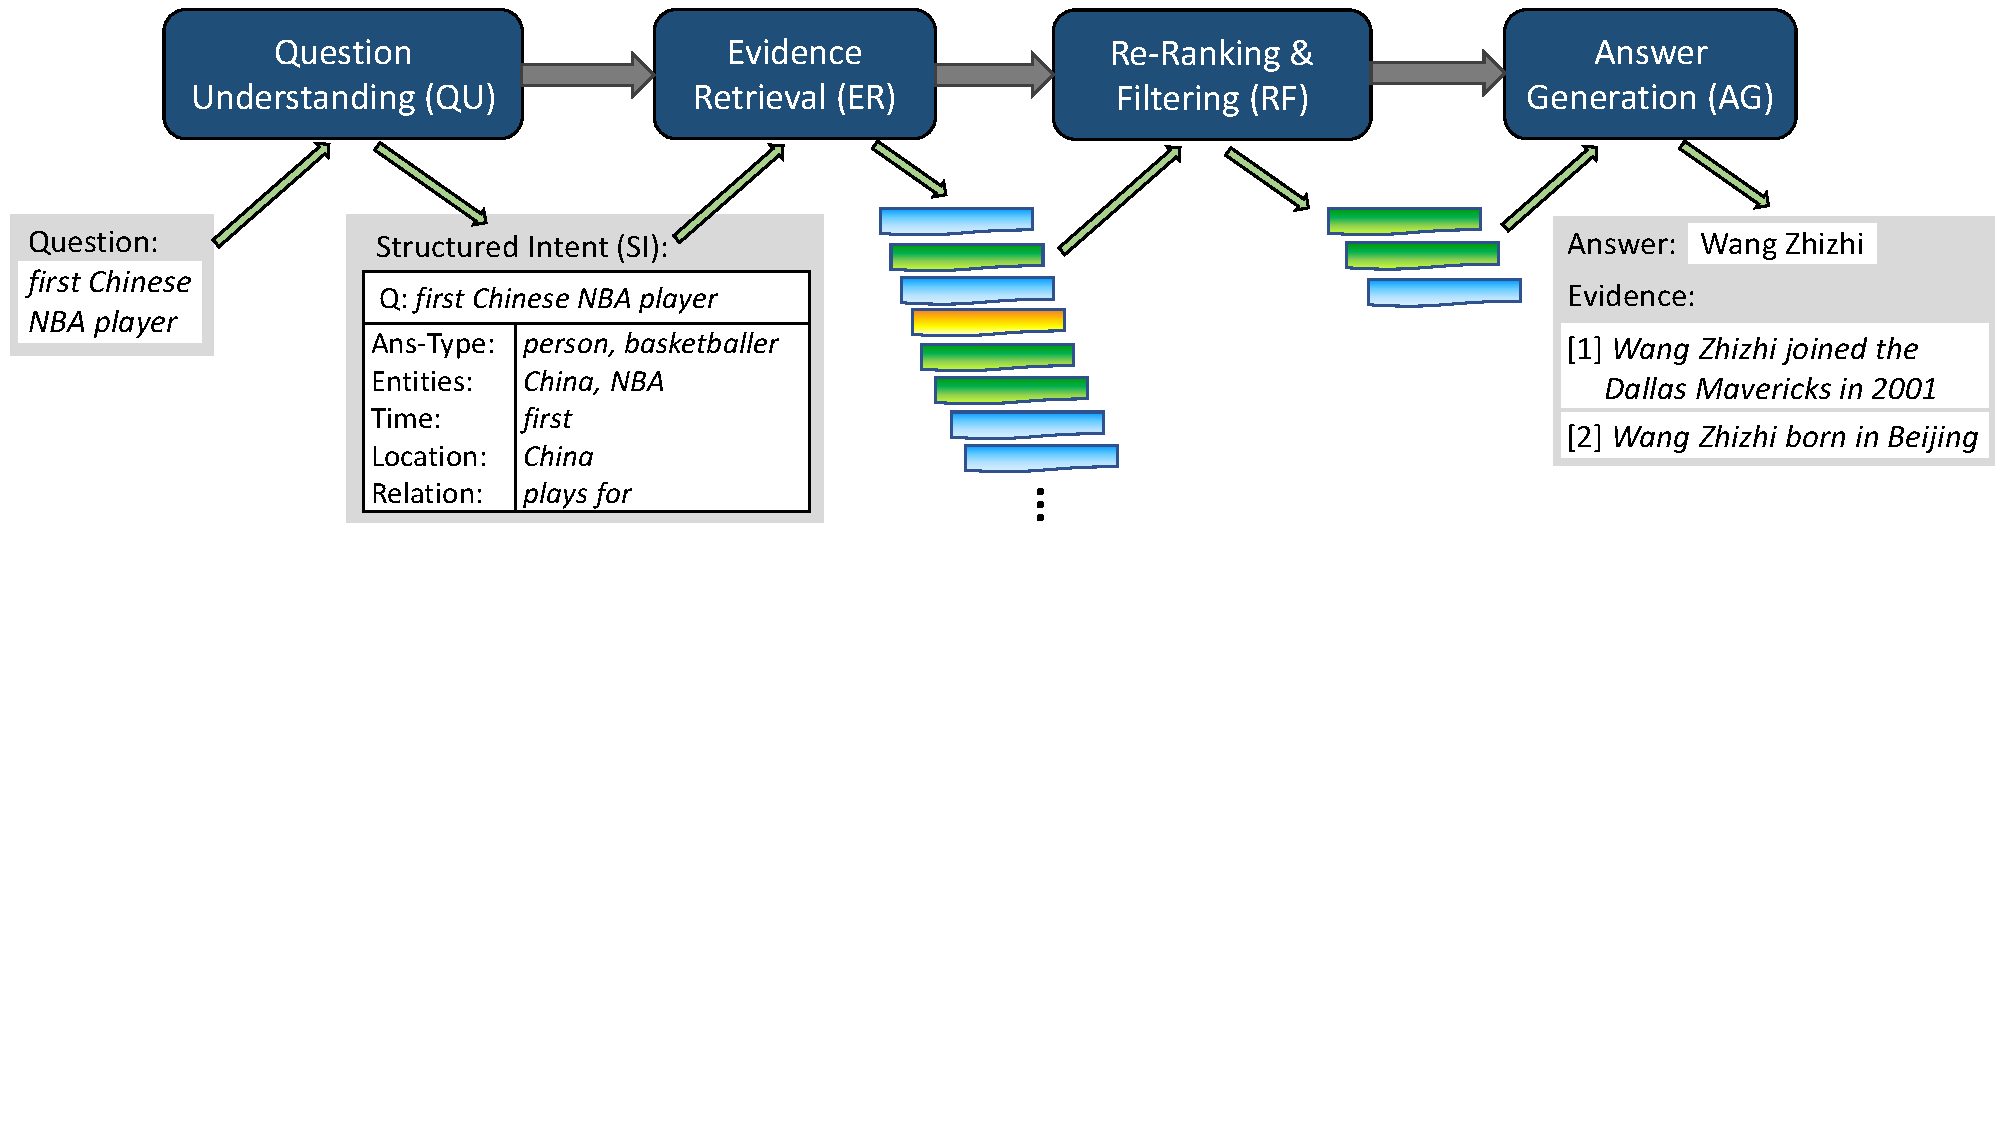
\includegraphics[width=\textwidth]{submissions/Gerhard2024/figures/compass-overview.pdf}
  \caption{Overview of the \method system.}
  \label{fig:compass-overview}
\end{figure}

% start with system overview
The \method system is a pipeline of four major stages, as illustrated in Figure \ref{fig:compass-overview}.
First, the input question is analyzed and decomposed, in order to compute a {\em structured intent (SI)} representation that will pass on to the subsequent steps, along with the original question. Second, the SI is utilized to retrieve pieces of evidence from different sources: text, KG and tables. 
Third, this pool of potentially useful evidence is filtered down, with iterative re-ranking, to arrive at a tractably small set of most promising evidence.
The final stage generates the answer from this evidence,
passing back the answer as well as evidence snippets for user-comprehensible explanation.

The second and fourth stage, Evidence Retrieval (ER) and Answer Generation (AG), are fairly standard. Such a two-phase architecture was called a retriever-reader architecture~\cite{Zhu-ODQA-survey:arxiv2021}. With a modern LLM replacing the earlier kinds of neural readers, this is the core of every RAG system~\cite{DBLP:journals/arXiv/abs-2312-10997}.

Stages 1 and 3 are unique elements of our architecture, judiciously introduced to improve both effectiveness (i.e., answer quality) and efficiency (i.e., computational cost).
Question Understanding (QU) provides the ER component with crisper and semantically refined input, and
the Re-Ranking \& Filtering (RF) stage is beneficial for
distilling the best evidence from the large pool of retrieved pieces.
The following subsections elaborate on the four stages of the pipeline, emphasizing the \method-specific steps QU and RF.



\subsection{Question Understanding (QU)}

% one par introducing the SI
To prepare the retrieval from different kinds of sources, including a KG, ad-hoc tables and text documents, it is useful to analyze and decompose the user question.
In this work, we aim to cast a question into a 
{\em structured intent (SI)} representation: essentially
a frame with faceted cues as slots, or equivalently, a concise set of key-value pairs. 
Figure \ref{fig:compass-overview} gives an idealized example for the question about the first Chinese NBA player. The facets or keys of potential interest here 
are:
\squishlist
\item {\em Ans-Type:} the expected answer type (or types when considering
different levels of semantic refinement), 
\item {\em Entities:} the salient entities in the question, and 
\item {\em Relation:} phrases that indicate which relation (between Q and A entities) the user is interested in. 
\squishend
\noindent In addition, as questions can have temporal or spatial aspects, the SI also foresees slots for:
\squishlist
\item {\em Time:} cues about answer-relevant time points or spans, including relative cues (e.g., ``before Covid'') and ordinal cues (e.g., ``first''), and
\item {\em Location:} cues about answer-relevant geo-locations.
\squishend

% discuss the spectrum of different SIs
\vspace{0.2cm}
\noindent The ideal SI for example question Q2 would look like:

\begin{quote}
{\em Ans-Type:} person, basketballer; {\em Entities:} China, NBA; {\em Time:} first;
{\em Location:} China; {\em Relation:} plays for.
\end{quote}

Note that the values for these slots can be crisp like entity names or dates, but they can also take the form of surface phrases. The SI purpose and value lie in the decomposition. In practice, many questions would only lead to a subset of faceted cues, leaving some slots empty. For the example in Figure \ref{fig:compass-overview}, an alternative SI could simply consist of

\begin{quote}
{\em Ans-Type:} person; {\em Entities:} China, NBA; {\em Time:} first.
\end{quote}

\noindent Even this simplified SI can be highly beneficial in guiding the subsequent evidence retrieval.

% sketch how an LM is trained to generate SIs 
To generate the SI from a user question, we employ a (small-scale) LM, specifically BART~\cite{DBLP:conf/acl/LewisLGGMLSZ20}, a Transformer-based auto-encoder with 140M parameters.\footnote{\url{https://huggingface.co/facebook/bart-base}}
BART is pre-trained for language representation; its power for our purpose comes from fine-tuning.
To this end, we generate (question, SI) pairs by using an instruction-trained LLM like GPT-4, with few-shot in-context learning (following our earlier work~\cite{Jia-FAITH:WWW2024}). 
Note that this is a one-time action; at inference-time we only use much smaller LMs.
The generated silver-standard pairs are then used to fine-tune BART.
In the experiments in this article, we leverage pre-existing collections of silver pairs, based on the training data of the CompMix benchmark~\cite{Christmann-CompMix:WWW2024}, 
comprising $3{,}400$ such pairs.


% outline value of SI for conversations
Although this paper focuses on single-shot questions, the \method architecture is also geared for conversational QA. In that setting, the SI can play an even bigger role, as (follow-up) questions are often formulated in a rather sloppy manner -- all but self-contained. For example, a conversation could start with a clear question {\em When did Wang Zhizhi join the NBA?}, followed a few dialog steps later, by a user utterance like {\em Which teams did he play for?} or simply {\em Which teams?}.
In such an informal conversation, the system needs to {\em contextualize} each user utterance based on the preceding turns in the dialog (e.g., inferring the relevant entities Wang Zhizhi and NBA from the conversational history).
For details on conversational QA, based on our architecture, see our earlier works~\cite{Christmann-CONVINSE:SIGIR2022,Christmann-Explaignn:SIGIR2023}.







%%%%%%%%%%%%%%%%%%%%%%%%%%%%%%%%%%%%%
\subsection{Evidence Retrieval (ER)}

The ER stage taps into a knowledge graph, a corpus of text documents, and a collection of web tables.
Specifically, for the experiments, we use the Wikidata KG,
all English Wikipedia articles, and all tables that are embedded in Wikipedia pages (incl. infoboxes, which can be seen as a special case of tables). 

% specifics: Clocq etc. - and the role of the SI
\vspace{0.2cm}
\noindent{\bf Retrieval from KG:}
To retrieve evidence from the KG, we utilize our earlier work
\clocq~\cite{Christmann-CLOCQ:WSDM2022}, which provides entity disambiguations and a relevant KG-subgraph for a given query.
Unlike most other works on QA-over-KG, \clocq fetches all KG-facts that are relevant for a given entity in a single step.
For example, when querying for
NBA players, it can traverse the KG neighborhood and pick up top teams, also considering so-called qualifier nodes in Wikidata which are often used for temporal scopes. 
As the disambiguation of entity names onto the KG can be tricky and noisy (e.g., China could be mapped to Chinese sports teams in all kinds of sports), \clocq considers several possible disambiguations~\cite{Christmann-CLOCQ:WSDM2022} (typically in the order of $10$ result entities).
The queries for \clocq are 
constructed by concatenating all slots of the question's SI.
For the example query about the first Chinese NBA player,
good result entities would be Dallas Mavericks, lists about NBA seasons, MVP awards etc., and their associated facts. These provide cues, but are likely insufficient to answer the question.


\vspace{0.2cm}
\noindent{\bf Retrieval from Text and Tables:}
The disambiguated entities returned by \clocq form anchors for tapping into text and tables.
\method first identifies 
relevant text documents and tables that refer to the anchor entities. With focus on Wikipedia, these are simply the articles for the respective entities. 
\method then constructs a keyword query that concatenates all available fields of the SI.
The query is evaluated against a linearized and verbalized representation (see below) of all sentences and all table rows in the selected documents.
This returns a set of sentences and 
and individual table rows, ranked by BM25 scores.


\vspace{0.2cm}
\noindent{\bf Evidence Verbalization:}
All results from the different data sources are uniformly treated by {\em linearizing} and {\em verbalizing} them
into token sequences. For KG results, the entity-centric triple sets are linearized via breadth-first traversal of the mini-graph starting from the entity node.
For tables, results are individual rows, which are contextualized by including labels from column headers and from the DOM-tree path of the article where the table comes from. For example, a table row about Wang Zhizhi playing for Dallas (Mavericks) in the 2000-2001 season, would be expressed as:

\vspace{0.05cm}
\hspace*{0.5cm} Wang Zhizhi / NBA Career / Season: 2000-2001, Team: Dallas, Games Played: 5 \dots
\vspace{0.05cm}

\noindent Finally, results from the text corpus are already in the form of token sequences, but we can additionally prefix these with the DOM-tree labels.
We can think of this entire pool of evidence as 
an on-the-fly corpus of potentially relevant pseudo-sentences, forming the input of the subsequent RF stage.


\vspace{0.2cm}
\noindent {\bf Result Ranking:}
Overall, the ER stage compiles a substantial set of evidence, possibly many thousands of entities, text snippets and table rows. Therefore, we practically restrict the pool to a subset of high-scoring pieces, like the top-$1000$.
For scoring, a simple BM25 model (a classical IR method) is applied. 
By default, we treat all evidence pieces uniformly with global scoring, no matter whether they come from KG, text or tables. 


\subsection{Re-Ranking and Filtering (RF)}

With a pool of top-$1000$ evidence pieces, we could invoke an LLM for answer generation. However, that would face a large fraction of noise (i.e., misleading evidence) and incur high costs of computation and energy consumption. 

For both of these reasons, we have devised light-weight techniques for iteratively reducing the top-$1000$ pieces to a small subset, say top-$30$ or top-$10$, that can be fed into an LLM at much lower cost (as LLM computations and pricing are at least linear in the number of input tokens). The difficulty is, of course, to do this without losing good evidence and reducing answer presence. Our techniques for this task are based on graph neural networks (GNNs)~\cite{Wu:IEEE2021} or cross-encoders (CEs)~\cite{Dejean:arxiv2024,Lin:MC2021}.

\myparagraph{GNN-based RF}
Given a large pool of evidence pieces from all sources, a bipartite graph is constructed:
\squishlist
\item {\em nodes} being evidence pieces or entities that occur in these pieces, and
\item {\em edges} connecting an evidence piece and an entity if the entity occurs in the evidence.
\squishend


The task for the GNN is to jointly score the evidence and the entity nodes in a multi-task learning setup. The latter are the {\em answer candidates}, and the evidence should give {\em faithful explanation} for an answer.
We build on our earlier work on explainable QA~\cite{Christmann-Explaignn:SIGIR2023}.

The node encodings are initialized with cross-encoder embeddings (see below) 
for node contents and the SI of the question. The inference iteratively adjusts the encodings based on message passing from neighboring nodes.
The GNN is trained via weak supervision from question-answer pairs:
evidence nodes are labeled as relevant if they are connected to
a gold answer.
More technical details are given in~\cite{Christmann-Explaignn:SIGIR2023}.

\method invokes the GNN in multiple rounds, iteratively reducing top-$k$ to top-$k^*$ nodes with $k^* \ll k$. In practice, we would typically consider two rounds: re-ranking top-$1000$ and pruning to top-100, and then reducing to top-30 or top-10, which are passed to the answer generation stage.
Note that this keeps the GNN at a tightly controlled size, so that its computational costs at inference-time are much smaller than those of an LLM.


\myparagraph{CE-based RF}
An alternative to the GNN inference is to employ a cross-encoder for scoring and re-ranking the evidence pieces.
These are transformers (typically with a small LM like BERT) that are fine-tuned for scoring the relatedness between a query and a document~\cite{Nogueira:arxiv2019}. In our case, the comparison is between the question SI and the evidence piece. In our experiments, we make use of two different cross-encoders, 
both trained on the MS-MARCO benchmark for passage retrieval~\cite{Bajaj:arxiv2018}, 
and fine-tuned on the respective benchmark (leveraging the same weak supervision data as for the GNNs),
the difference being in model size.\footnote{\url{https://huggingface.co/cross-encoder/ms-marco-MiniLM-L-4-v2} and\\ \url{https://huggingface.co/cross-encoder/ms-marco-MiniLM-L-6-v2}}
We use the smaller model to reduce top-$1000$ to top-100, and the larger model to go further down from top-100 to top-30.




%%%%%%%%%%%%%%%%%%%%%%%%%%%%%%%%%%%%%

\subsection{Answer Generation (AG)}

The last stage follows mainstream practice to invoke an LLM in a retrieval-augmented manner.
We call a `small-scale` LLM, specifically a fine-tuned LlaMA-3.1 model (8B-Instruct)\footnote{\url{https://huggingface.co/meta-llama/Llama-3.1-8B-Instruct}}, with a prompt \footnote{The specific prompt is \phrase{SI: \textless\texttt{concatenated SI}\textgreater \hspace{0.1cm} Evidence: \textless\texttt{evidence pieces}\textgreater}.}
consisting of:

\squishlist
\item the concatenated SI of the original question, and
\item the top-30 (or other top-$k^*$ with small $k^*$) evidence pieces.
\squishend

By the previous down-filtering of the original pool of evidence pieces, this last step has affordable cost in terms of computation time and energy consumption.

\vspace{0.2cm}
\noindent{\bf Fine-Tuning the LLM:}
We considered adding an instruction to the prompting, such as {\em ``answer this question solely based on the provided evidence snippets''}.
However, this turned out to be ineffective.
The reason why the model works well without such instructions is our task-specific fine-tuning.
We perform this by running the training data of benchmarks through the \method pipeline,
and training the AG stage with the top-30 evidence pieces as input.
Thus, the fine-tuning makes the model learn the role of evidence for RAG-based QA.

\vspace{0.2cm}
\noindent{\bf Explanations:}
The top-30 evidence pieces can be used to provide users with explanation of answers.
Optionally, these could be reduced further for comprehensibility.
Alternatively, we can fine-tune the LLM to provide both answers and concise explanations.
Since we can infer which evidences in the input mention the annotated ground-truth answers,
our method could be fine-tuned to provide such \textit{answering evidences} as well (cf.~\cite{Gao-citations:emnlp2023}).

\label{sec:exp}
\section{Experiments}


\label{setup}
\subsection{Experimental setup}


%%% BENCHMARKS
\myparagraphnospace{Benchmarks} We run experiments on three benchmarks with different characteristics of questions.

\squishlist
    \item \textbf{\compmix}.
    \compmix~\cite{Christmann-CompMix:WWW2024} is a benchmark which was specifically designed for evaluating QA systems operating over heterogeneous sources. The dataset has $9{,}410$ questions, out of which $2{,}764$ are used for testing.
    Answers are crisp entity names, dates, or other literals.
    
    \item \textbf{\crag}.
    We further evaluate on a subset of the \crag~\cite{Yang-CRAG} dataset, which was recently released as a testbed for RAG-based QA systems.
    We utilize the same pipeline and sources as outlined in Section~\ref{sec:method}, without using the web snippets or APIs provided with \crag. This way we focus on entity-centric questions that do not require access to live web data (e.g., news feeds), and disregard cases where the results would be up-to-date quantities.
    This restricts the test data to $436$ entity-centric questions, still enough for a proof of concept.
    
    \item \textbf{\timequestions}.
    To showcase the generalizability of our pipeline, we conduct experiments on~\timequestions~\cite{Jia-TimeQuestions},
    a benchmark for temporal QA. The dataset requires temporal understanding and reasoning, which are well-known limitations of
    LLMs~\cite{Dhingra-time-aware-LLM:TACL2022}. \timequestions has 16{,}181 questions (3{,}237 for testing).
\squishend

Typical examples for the questions in these three benchmarks are:

\begin{quote}
\compmix: \utterance{Which player won the most number of Man-of-the-Match titles in the FIFA world cup of 2006?}\\
 \indent \crag: \utterance{What was the worldwide box office sales for little hercules?}\\ 
  \indent \timequestions: \utterance{Which club did Cristiano Ronaldo play for before joining Real Madrid?}
\end{quote}

%%% BASELINES
\myparagraph{Baselines} As competitors or reference points to \method, we study the performance of the following methods:

\squishlist
    \item \textbf{Generative LLMs}.
    We compare \method against out-of-the-box LLMs: \textbf{\gptthree} (\texttt{text-davinci-003}), \textbf{\gptfour} (\texttt{gpt-4}) 
    and \textbf{\llama} (\texttt{meta-llama/Llama-3.1-8B-Instruct}).
    The same prompt is used for all LLMs, consistent with previous work~\cite{Christmann-CompMix:WWW2024, Zhang-Spaghetti:ACL2024}:
    \phrase{Please answer the following question by providing the crisp answer entity, date, year, or numeric number. Q: \textless\texttt{question}\textgreater}.
    

    \item \textbf{Heterogeneous QA methods}.
    \convinse~\cite{Christmann-CONVINSE:SIGIR2022}, \unikqa~\cite{Oguz-UniK-QA:NAACL2022}, \explaignn~\cite{Christmann-Explaignn:SIGIR2023}
    are QA methods designed to integrate heterogeneous sources: text, tables and KG. All of these  integrate the exact same sources as \method.

    
    \item \textbf{\textsc{State-of-the-art}}.
    For \compmix and \timequestions, we also compare against state-of-the-art methods from the literature: \spaghetti~\cite{Zhang-Spaghetti:ACL2024} and \textsc{Un-Faith}~\cite{Jia-FAITH:WWW2024}, which are among the best performing systems.
    
Results are taken from the literature whenever applicable.
On \crag, we use the models trained on \compmix for \method and heterogeneous QA baselines.
\squishend



%%% METRIC(S)
\myparagraph{Metrics}
We measure \textit{precision at 1} (\textbf{P@1}) as our main metric~\cite{RoyAnand:MC2021} on all benchmarks.
On \crag, we manually annotate answer correctness, as the ground-truth answer formats vary (e.g., entity name variants, lists, sentences).

We also compute the number of neural parameters aggregated over all sub-modules (\textbf{\#Parameters}).
Parameter counts for GPT-models are taken from~\cite{Minaee-LLM-survey}
(\gptfour might have less active parameters during inference).

For further analysis we measure \textit{answer presence} (\textbf{AP@k}),
i.e. whether the answer is present in the top-$k$ ranked evidence pieces,
and \textit{mean reciprocal rank} within the top-$k$ evidences (\textbf{MRR@k}).

%%% CONFIG
\myparagraph{Configuration}
Our implementation uses the \texttt{Llama3.1-8B-Instruct} model for the AG stage.
For the QU, ER and RF stages
we adopt code from the \explaignn project.\footnote{\url{https://explaignn.mpi-inf.mpg.de}}
For the ER stage, we use \clocq, setting its specific parameters to $k=10$ and $p=1{,}000$.

As default, we use the GNN technique for the RF stage.
For efficiency, we use light-weight models for initializing
the GNN encoders -- the same models used for the CE-based RF.\footnote{\url{https://huggingface.co/cross-encoder/ms-marco-MiniLM-L-4-v2} and\\\url{https://huggingface.co/cross-encoder/ms-marco-MiniLM-L-6-v2}}
The GNNs are trained for $5$ epochs with an epoch-wise evaluation strategy,
i.e. we choose the model with the best performance on the respective dev set.
We train the GNNs on graphs with a maximum of $100$ evidence and $400$ entity nodes (as scored by BM25).
During inference, the first GNN is applied on graphs with $1{,}000$ evidence and $4{,}000$ entity nodes, shrinking the pool of evidence pieces to the top-$100$.
The second GNN then runs on graphs with $100$ evidence and $400$ entity nodes.
The factor of 4 entities per evidence (on average) holds sufficient for the observed data,
and enables batched inference.
Other parameters are kept as is.

The AG model, based on \texttt{Llama3.1-8B-Instruct}, is 
fine-tuned
for $2$ epochs with a warm-up ratio of $0.01$ and a batch size of $8$, again with an epoch-wise evaluation strategy.
Other parameters are set to the default Hugging Face
training parameters.\footnote{\url{https://huggingface.co/docs/transformers/v4.46.2/en/main_classes/trainer\#transformers.TrainingArguments}}





\subsection{Main results}
%%% MAIN TABLE
\myparagraphnospace{\method is competitive on all benchmarks}
Main results of our experiments are shown in Table~\ref{tab:main-res}.
First of all, we note that \method achieves competitive performance across all three benchmarks.

On \compmix, baselines for heterogeneous QA and \llama perform similarly,
whereas GPT-based LLMs can answer more than $50$\% of the questions correctly.
\method exhibits substantially higher performance, on par with
the state-of-the-art method \textsc{Spaghetti}~\cite{Zhang-Spaghetti:ACL2024}
(which is based on \gptfour).

On the \crag dataset, P@1 drops for all methods except for \gptfour. 
The benchmark includes realistic questions,
which can be ambiguous/confusing (\phrase{who was the director for the report?}),
on ``exotic'' entities with answers in social media (\phrase{how many members does the teknoist have?}),
or require up-to-date information (\phrase{when did chris brown release a song or album the last time?}),
and other cases that are challenging for all methods.

Finally, \method establishes new state-of-the-art performance on the \timequestions benchmark.
Interestingly, all of the tested LLMs show greatly reduced performance on this benchmark,
which inherently requires temporal understanding and reasoning
-- a known weakness of stand-alone LLMs.


\begin{table} [h]
    \centering
    \newcolumntype{G}{>{\columncolor [gray] {0.90}}c}
    \begin{tabular}{l G G G c}
        \toprule
            \textbf{Method $\downarrow$ / Benchmark $\rightarrow$} & \textbf{\compmix}  & \textbf{\crag} & \textbf{\timequestions} & \textbf{\#Parameters} \\ 
        \midrule
            \textbf{\gptthree} 
            & $0.502$ &   $-$ & $0.224$ & $175{,}000$ M  \\
            % #params from https://arxiv.org/pdf/2402.06196

            \textbf{\gptfour}
            & $0.528$ &   $\mathbf{0.633}$ & $0.306$ & $1{,}760{,}000$ M \\
            % #params from https://arxiv.org/pdf/2402.06196

            \textbf{\llama~\cite{Touvron-LLaMA}} (8B-Instruct)
            & $0.431$ &   $0.385$ & $0.178$ & $8{,}030$ M  \\
            % #params from Huggingface (8,030,257,152)
        \midrule
            \textbf{\convinse~\cite{Christmann-CONVINSE:SIGIR2022}}
            & $0.407$  &   $0.298$ & $0.423$  & $362$ M \\
            % FiD: 222,903,936 + BART (SR-generation): 139,420,416 = 362,324,352 (python explaignn/question_understanding/structured_representation/get_num_params.py)

            \textbf{\unikqa~\cite{Oguz-UniK-QA:NAACL2022}}
            & $0.440$ &   $0.280$ & $0.424$ & $223$ M  \\
            % FiD: 222,903,936 (python explaignn/heterogeneous_answering/fid_module/FiD/get_num_params.py)
    
            \textbf{\explaignn~\cite{Christmann-Explaignn:SIGIR2023}} 
            & $0.442$ &   $0.303$ & $0.525$  & $328$ M \\
            % BART (SR-generation): 139,420,416 + 2GNNs: 94520832 + 93930240 = 327,871,488

        \midrule 
            \textbf{\textsc{State-of-the-art}}
            & $\mathbf{0.565}$ 
            & $-$
            & $0.571$  & $-$ \\

            & (\textsc{Spaghetti}~\cite{Zhang-Spaghetti:ACL2024})
            & 
            & (\textsc{Un-Faith}~\cite{Jia-FAITH:WWW2024}) &  \\

        \midrule
            \textbf{\method (ours)}
            & ${0.564}$ &   $0.362$ & $\mathbf{0.754}$  & $8{,}218$ M \\
            % BART (SR-generation): 139,420,416 + LLaMA: 8,030,257,152 + GNNs: 25,670,016 + 22,268,928 =  8,217,616,510
        \bottomrule
    \end{tabular} 
    \vspace*{-0.2cm}
    \caption{End-to-end P@1 of \method and baselines on three benchmarks. Results for \gptthree and \gptfour are taken from the literature~\cite{Christmann-CompMix:WWW2024, Jia-FAITH:WWW2024}. \gptthree is not accessible anymore, hence no results on \crag.
    }
    \label{tab:main-res}
\end{table}





%%% ANSWER SOURCES
\myparagraph{Integration of heterogeneous sources is vital}
\method integrates evidence from text, KG and tables into a unified framework.
We aim to better understand how this affects the answering performance of the method.
Table~\ref{tab:sources} shows end-to-end answering performance of \method
with different combinations of the input sources.
The results clearly indicate that all types of sources contribute, with option Text+KG+Tables performing best,
with a large margin over tapping only single source types.

\begin{table} [t] 
    \centering
    \newcolumntype{G}{>{\columncolor [gray] {0.90}}c}
    \newcolumntype{H}{>{\setbox0=\hbox\bgroup}c<{\egroup}@{}}
    	\begin{tabular}{l G G G H H H c c c} 
        \toprule
            \textbf{Benchmark $\rightarrow$}
                & \multicolumn{3}{G}{\textbf{\compmix}} 
                & \multicolumn{3}{H}{\textbf{\crag}}
                & \multicolumn{3}{c}{\textbf{\timequestions}} \\ 
        \midrule
            \textbf{Input sources $\downarrow$ / Metric $\rightarrow$}
                & \textbf{P@1} & \textbf{AP@100}  & \textbf{AP@30}
                & \textbf{P@1} & \textbf{AP@100}  & \textbf{AP@30}
                & \textbf{P@1} & \textbf{AP@100}  & \textbf{AP@30} \\
            \midrule
                \textbf{Text}           &  $0.455$  &  $0.563$  &  $0.531$ &  $?$  &  $?$  &  $?$ &  $0.539$  &  $0.515$  &  $0.487$   \\
                \textbf{KG}             &  $0.481$  &  $0.677$  &  $0.637$ &  $?$  &  $?$  &  $?$ &  $0.724$  &  $0.701$  &  $0.674$   \\
                \textbf{Tables}         &  $0.432$  &  $0.501$  &  $0.482$ &  $?$  &  $?$  &  $?$ &  $0.536$  &  $0.347$  &  $0.328$   \\
            \midrule
                \textbf{Text+KG}        &  $0.537$  &  $0.749$  &  $0.706$ &  $?$  &  $?$  &  $?$ &  $0.745$  &  $\mathbf{0.776}$  &  $0.748$   \\
                \textbf{Text+Tables}    &  $0.503$  &  $0.632$  &  $0.594$ &  $?$  &  $?$  &  $?$ &  $0.567$  &  $0.578$  &  $0.549$   \\
                \textbf{KG+Tables}      &  $0.524$  &  $0.728$  &  $0.692$ &  $?$  &  $?$  &  $?$ &  $ 0.743$  &  $0.731$  &  $0.703$   \\
            \midrule
                \textbf{Text+KG+Tables}    &  $\mathbf{0.564}$  &  $\mathbf{0.759}$  &  $\mathbf{0.724}$ &  $?$ &  $?$  &  $?$ & $\mathbf{0.754}$    & $\mathbf{0.776}$  &  $\mathbf{0.749}$   \\
            \bottomrule
    \end{tabular}
    \vspace*{-0.2cm}
    \caption{Answer presence and answering precision of \method with different combinations of input sources (on the respective test sets).}
    \label{tab:sources}
\end{table}




\subsection{Analysis}

%%% TOP-K vs. 3xTOP-(K/3)
\myparagraph{Unified retrieval enhances performance}
In the RF stage, we re-rank and filter evidence from different source types,
and feed the unified top-\textit{k}* into the AG stage.
We conduct a comparison in which we consider
the top-$10$ evidence pieces from each source type individually. This gives equal influence to KG, text and tables, whereas our default is based on global ranking.
Table~\ref{tab:unified-retrieval} shows the results for this analysis, showing our default choice performs better.
The reason is that different questions require different amounts of evidence from each of the source types.

\begin{table} [t] 
    \centering
    \newcolumntype{G}{>{\columncolor [gray] {0.90}}c}
    \newcolumntype{H}{>{\setbox0=\hbox\bgroup}c<{\egroup}@{}}
    	\begin{tabular}{l G G H H} 
        \toprule
            \textbf{Input evidences $\downarrow$ / Metric $\rightarrow$} & \textbf{P@1} & \textbf{AP@30}  & \textbf{\crag} & \textbf{\timequestions} \\ 
            \midrule
                \textbf{Top-30 Text+KG+Tables (ours)}             &  $\mathbf{0.574}$  &  $\mathbf{0.710}$  &  $-$  &  $-$   \\
                \textbf{Top-10 Text + Top-10 KG + Top-10 Tables}        &  $0.560$    &  $0.709$  &  $-$  &  $-$   \\
            \bottomrule
    \end{tabular}
    \vspace*{-0.2cm}
    \caption{Answer presence and precision
    of \method for different choices of top-30 
    (on \compmix dev set).}
    \label{tab:unified-retrieval}
\end{table}


%%% NUMBER OF EVIDENCES
\myparagraph{\method works well with small amounts of evidence}
We investigate the 
influence of 
the number of evidence pieces
fed into the AG stage, varying it from $5$ to $100$.
Results are shown in Figure~\ref{fig:res-num-evidences}.
As the curve shows, there is a sharp increase in precision as we add evidence up to 30 or 40 pieces, which is around our default of top-30. This indicates that a certain amount of evidence is needed, to overcome the inherent noise and arrive at sufficient answer presence. 
As we increase the amount of evidence further, we observe a saturation effect, and eventually a degration of performance. Too much evidence not only has diminishing returns, but can actually be confusing for the AG stage. This reconfirms our heuristic choice of top-30: enough for good answering while keeping computational costs reasonably low.


\begin{figure}[t]
    \centering
    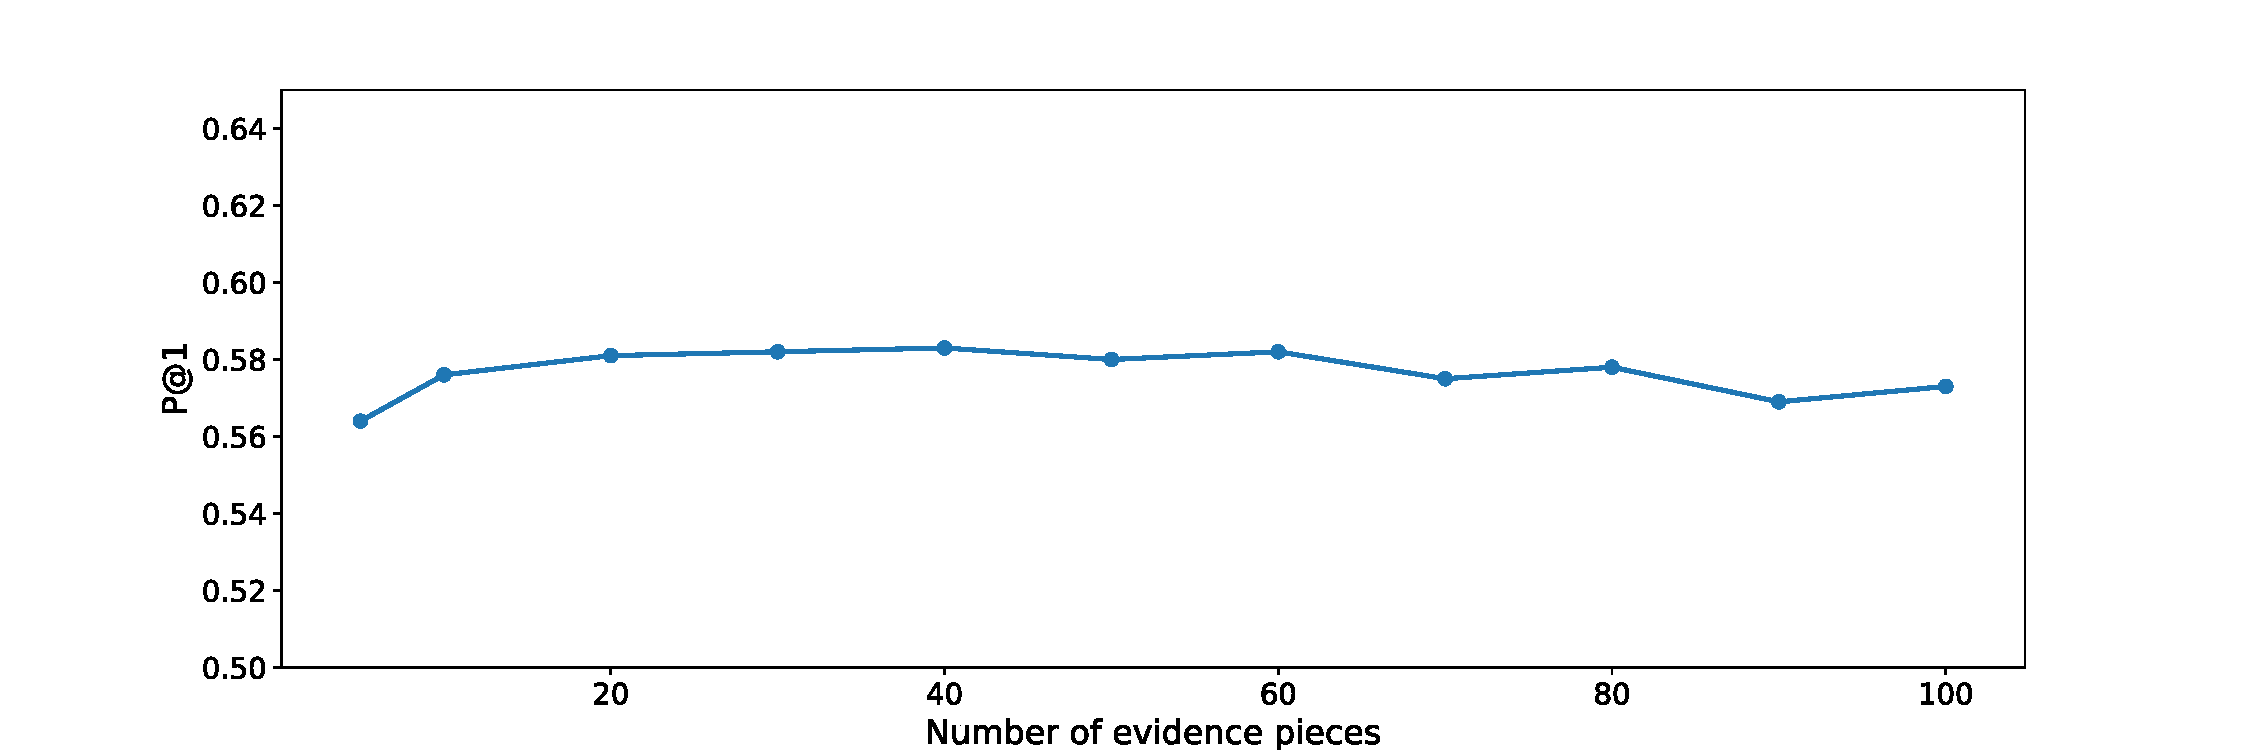
\includegraphics[width=0.8\textwidth]{submissions/Gerhard2024/figures/p_at_1-line_with_evidences.pdf}
    \vspace*{-0.2cm}
    \caption{Performance of \method on the \compmix dev set with different numbers of evidence.}
    \label{fig:res-num-evidences}
    \vspace*{-0.2cm}
\end{figure}



%%% ABLATION
\myparagraph{Ablation study on re-ranking} For more insight on the possible configurations of the RF stage, we conducted an ablation study with different options, including solely relying on the initial BM25 scoring without explicit re-ranking. The results are shown in Table \ref{tab:ablation2}. We observe that the iterative reduction in two steps is slightly better than the single-step variants (going down from top-1000 to top-30 in one RF step). Between the two options of using a GNN or a CE, the differences are negligible. A notable effect is that our RF techniques retain the answer presence at a very high level, only a bit lower than for the initial top-1000. 
The last two rows of Table \ref{tab:ablation2} demonstrate that RF is crucial: without explicit re-ranking, the technique of just picking smaller top-$k$ from the original BM25 model leads to substantial degradation in both answer presence and precision. 


\begin{table} [t] \small
    \centering
    \newcolumntype{G}{>{\columncolor [gray] {0.90}}c}
    \newcolumntype{H}{>{\setbox0=\hbox\bgroup}c<{\egroup}@{}}
    	\begin{tabular}{l G H G G G} 
        \toprule
            & \multicolumn{5}{G}{\textbf{\compmix} (dev set)} \\
        \midrule
            \textbf{RF Method $\downarrow$ / Metric $\rightarrow$} & \textbf{P@1} & \textbf{AP@1000} & \textbf{AP@100}  & \textbf{AP@30} & \textbf{MRR@100} \\ 
        \midrule
            \textbf{GNN: 1000 $\rightarrow$ 100 $\rightarrow$ 30}             &  $\mathbf{0.574}$  & $0.760$ &  $0.738$  &  $0.710$  &  $\mathbf{0.572}$  \\
            \textbf{CE: 1000 $\rightarrow$ 100 $\rightarrow$ 30}          &  $0.573$  & $0.760$  &   $\mathbf{0.740}$ &  $\mathbf{0.721}$   &  $0.553$   \\
        \midrule
            \textbf{GNN: 1000 $\rightarrow$ 30} &  $0.567$  & $?$  &   $n/a$ &  $0.710$   &  $0.567$   \\
         \textbf{CE: 1000 $\rightarrow$ 30} &  $0.570$  & $0.760$  &   $n/a$ &  $0.715$   &  $0.558$   \\
            \midrule
           \textbf{BM25: 100 (w/o GNN or CE)} &  $0.490$ & $0.760$  &  $0.652$  &  $n/a$  &  $0.259$ \\       
            \textbf{BM25: 30 (w/o GNN or CE)} &  $0.468$  & $0.760$  &  $n/a$ &  $0.534$   &  $0.259$   \\
            \bottomrule
    \end{tabular}
    \vspace*{-0.2cm}
    \caption{Ablation study for different RF strategies of \method on the \compmix dev set. The answer presence in the RF input with top-$1000$ evidence pieces is $0.760$.}
    \label{tab:ablation2}
\end{table}



\myparagraph{Quality of SI}
To assess the quality and robustness of the Structured Intents, we
inspected a sample of questions and their SIs.
Table~\ref{tab:question-SI-examples} gives three anecdotic examples.
We show SIs generated by \method, which makes use of the pre-existing collection from the \compmix benchmark for training.
This training data was obtained via different heuristics, 
which can be a limiting factor when user intents become more complex.

Therefore, we also looked at SIs derived via in-context learning (ICL) using \gptfour with $5$ handcrafted examples.
As shown in our earlier work on temporal QA~\cite{Jia-FAITH:WWW2024},
such data can be used for training smaller models (e.g., BART),
which can greatly boost the completeness and overall quality of the generated SIs.

From the sampled set, we observed that the ICL-based SIs are more
complete with all slots filled, whereas the BART-based SIs focused more
on the main slots Answer-type, Entities and Relation.
However, both approaches achieve very high quality in filling the slots,
capturing the user's information need very well.

Interestingly, when questions get complicated, with nested phrases, 
the ICL-based variant succeeds in decomposing the questions, based on only $5$ ICL examples.
For example, for the question {\em ``which German state had the most Corona-related death cases in the first year after the outbreak?''}
the Time slot becomes {\em ``first year after Corona outbreak''},
which can be resolved to identify the temporal scope.
In general, we believe that such question decomposition, beyond simple temporal constraints,
would be an interesting theme for future work.

\begin{table} [t] 
    \centering
    \small
    \newcolumntype{G}{>{\columncolor [gray] {0.90}}c}
    \newcolumntype{H}{>{\setbox0=\hbox\bgroup}c<{\egroup}@{}}
    \resizebox*{\textwidth}{!}{
        \begin{tabular}{p{6cm}|p{6cm}|p{6cm}} 
        \toprule
            \textbf{Question} & \textbf{Current SI by \method} & \textbf{SI via ICL} \\
        \midrule
        \textit{what was disneys first color movie?}
            & Ans-Type: \textit{animated feature film} & Ans-Type: \textit{film, animated film} \\
            & Entities: \textit{disneys} & Entities: \textit{Disney} \\
            & Relation: \textit{was first color movie} & Relation: \textit{first color movie} \\
            &  & Time: \textit{first} \\
        \midrule
        \textit{at the oscars, who won best actor in 2018?}
            & Ans-Type: \textit{human} & Ans-Type: \textit{person, actor} \\
            & Entities: \textit{at the oscars} & Entities: \textit{Oscars, 2018} \\
            & Relation: \textit{who won best actor in 2018} & Relation: \textit{won best actor} \\
            &  & Time: \textit{2018} \\
        \midrule
        \textit{which German state had the most Corona-} & Ans-Type: \textit{state} & Ans-Type: \textit{location, state} \\
        \textit{related death cases in the first year after} & Entities: \textit{Germany, Corona} & Entities: \textit{Germany, Corona-related deaths} \\
        \textit{the outbreak?} & Relation: \textit{which state had the most related} & Relation: \textit{highest count of death cases} \\
        & \textit{death cases in the first year after the out-}  & Location: \textit{Germany} \\
            & \textit{break}  & Time: \textit{first year after Corona outbreak} \\
        \bottomrule
    \end{tabular}
    }
    \vspace*{-0.2cm}
    \caption{Examples for pairs of question and generated SI.}
    \label{tab:question-SI-examples}
\end{table}




%%% REFRAIN FROM ANSWER
\myparagraph{Refraining from answering}
%%% Searched for: "generated_answer I" (with I being the full word, not partial) in the generated answers of LLaMA
%%% yields 245 results out of 2764 questions on CompMix
%%% yields 1270 results out of 3237 questions on TimeQuestions
We can train our model to refrain from answering in scenarios
where the provided evidence does not contain an answer to the question.
Specifically, during training, when the answer is not present in the evidence,
we change the target answer to {\em unknown}. This variant is referred to as \method {\em (faithful)}.

We measure the ratio of questions for which {\em unknown} is provided as answer,
and the P@1 restricted to questions that are answered.
The accuracy of refraining from answering is measured as well,
based on whether the answer is present in the evidence or not.
We conduct this experiment on \compmix and \timequestions,
for which we can compute answer presence exactly.
We also compute results for \llama, which is already instructed 
with the option to answer ``don't know''.
Table~\ref{tab:refrain-from-answer} shows the results.
For \compmix, we observe that \method has high accuracy on refraining when appropriate,
whereas \llama tends to be overconfident with a very small rate of {\em unknowns}, leading to incorrect answers.

\begin{table} [t] \small
    \centering
    \newcolumntype{G}{>{\columncolor [gray] {0.90}}c}
    \newcolumntype{H}{>{\setbox0=\hbox\bgroup}c<{\egroup}@{}}
    	\begin{tabular}{l G G G G c c c c} 
        \toprule
            & \multicolumn{4}{G}{\textbf{\compmix}} & \multicolumn{4}{c}{\textbf{\timequestions}} \\
            \midrule
            \textbf{Metric $\rightarrow$} & \textbf{P@1}  & \textbf{P@1} & \textbf{Refrain} & \textbf{Refrain} & \textbf{P@1}  & \textbf{P@1} & \textbf{Refrain} & \textbf{Refrain} \\ 
            \textbf{Method $\downarrow$} &                 & \textbf{(answered)} & \textbf{rate} & \textbf{accuracy} &                 & \textbf{(answered)} & \textbf{rate} & \textbf{accuracy} \\ 
            \midrule
                \textbf{\llama}             &  $0.431$  &  $0.471$  &  $0.089$  &  $n/a$  &  $0.177$  &  $0.276$  &  $0.392$  &  $n/a$  \\
                \textbf{\method (faithful)}           &  $0.497$  &  $0.713$  &  $0.303$  &  $0.838$ &  $0.597$  &  $0.804$  &  $0.257$  &  $0.864$  \\
            \bottomrule
    \end{tabular}
    \vspace*{-0.2cm}
    \caption{
        Performance of \method with option to refrain from answering (``don't know'').
    }
    \label{tab:refrain-from-answer}
\end{table}

\label{sec:disc}
\section{Insights, Limitations, and Challenges}


\noindent{\bf Benchmark Performance.} Our method, RAG-based \method with an 8B LLaMA model, outperforms much larger LLMs like \gptfour on two of the three benchmarks, with a very large margin for temporal questions. Obviously, pre-trained LLMs have only limited sense of properly positioning ``remembered’’ facts on the timeline even with training data that exceeds ours by several orders of magnitude. This confirms our intuition that LLMs alone are not good at ``recalling’’  higher-arity relations that require combining distant pieces of evidence. This is a sweet spot for RAG. Only for 
the \crag benchmark, \method is substantially inferior to a full-blown LLM. This is likely due to the nature of the questions: not necessarily the complexity of the information needs, but the need for more web sources (beyond what our experiments tap into).

\vspace{0.2cm}
\noindent{\bf Cost/Performance Ratio.} The most important take-away from our experiments is that \method achieves its competitive performance at a much lower cost than the full LLMs. Assuming that the consumed GFlops are proportional to the number of model parameters, \method achieves a cost reduction by a factor of 200x for \gptthree and 2000x for \gptfour. This does not only mean less computation, but also a massively lower electricity bill and climate impact.  

\vspace{0.2cm}
\noindent{\bf Role of Question Understanding.} We did not systematically investigate the influence of the Structured Intent in the \method pipeline. However, the comparison to the big GPT models reflects the role of the SI, as we prompt the GPT models in their natural mode with the original questions. The linearized sequence of available SI slots does not always have major advantages, but there are enough cases where specific facets provide crucial cues. This holds especially for the Entities slot, as this drives the gathering of evidence in the ER stage (cf.~\cite{Christmann-CONVINSE:SIGIR2022}, and for the Time slot, as these cues are often decisive for temporal questions (cf.~\cite{Jia-FAITH:WWW2024}).

\vspace{0.2cm}
\noindent{\bf Role of Re-Ranking.} As our ablation studies show, merely using top-$k$ evidence from an initial BM25-style ranking does not provide good performance. Also, there seems to be sweet spot in the choice of $k$: we need enough evidence for connecting the dots if the question requires multiple pieces of information, or for corroborating candidates if the question finds many useful but noisy pieces. In the experiments, $k=30$ turns out to be good choice; much lower $k$ results in insufficient evidence, and much larger $k$ leads to saturation and ultimately degrading performance. Our argument for iteratively shrinking the candidate set in multiple rounds of re-ranking is substantiated in our experiments, but the gain of doing this, compared to GNN- or CE-based re-ranking from 1000 to 30, is not big. More research is called to better understand the role of ranking in RAG. 

\vspace{0.2cm}
\noindent{\bf Limitations of Evidence Retrieval.}
For ER, we adopted more or less standard techniques. The results showed very good answer presence, in the order of 75\% in the top-100 or even top-30. An important case where this is insufficient are questions that require aggregating information over a large number of evidence pieces. An example is asking for the life-time total of 3-point scores of the basketball player Dirk Nowitzki.
This requires collecting a set of per-season tables with NBA player statistics, but also other web sources with numbers for his career before he joined the NBA (including his youth teams).
Of course, there are sometimes shortcuts like a Wikipedia article or biography mentioning the total number, but this cannot be universally assumed. The bottom line is that ER should be reconsidered as well, striving to improve the recall dimension.

\vspace{0.2cm}
\noindent{\bf Limitations of Answer Generation.}
For AG, we simply rely on a LLM,
using it as an extractor (``reader'') from the given evidence. Despite the wide belief that LLMs can perform deep
reasoning over many pieces of evidence, our experience is that the extraction works only well – robustly and faithfully – for relatively simple questions with a few multi-hop joins or simple aggregation over a few pieces. However, complicated questions such as asking for the top-100 NBA players with the largest number of life-time 3-point scores (again including their pre-NBA careers) are currently out of scope and will likely remain so for quite some time. This offers many opportunities for pushing the envelope further.

\vspace{0.2cm}
\noindent{\bf Trust in Data Sources.}
In our experiments, we considered all heterogeneous sources as trustworthy and unbiased. With focus on Wikidata and Wikipedia, this assumption has been well justified. In the wild, however, input data for RAG-based systems likely exhibit a wide spectrum of quality issues, in terms of stale information, biased positions, or simply false statements. Identifying trustworthy and up-to-date evidence and dealing with conflicting data, has been explored in other contexts (e.g., for KG curation~\cite{Dong-Trust:PVLDB2015}), but remains a major challenge for RAG-based QA.


\vspace{0.2cm}
\noindent{\bf Open Challenges and Future Work.} The best-performing methods in our experiment, mostly \method, reach P@1 values of 56\% for \compmix and 75\% for \timequestions. 
For the latter, the answer presence in the top-100 is only slightly higher; so the AG stage hardly misses anything.
However, for \compmix, the answer presence is 75\% -- much higher than what our system can actually answer. Obviously, closing this gap is a major direction to pursue, with focus on the RF and AG stages. However, missing one fourth of the answers completely in the top-100 pool, is a big problem as well. This requires improving recall at the ER stage, possibly with better guidance by the QU, which in turn needs more sources beyond the scope of our experiments (currently limited to Wikidata and Wikipedia). 

In general, we need to think beyond this kind of ``benchmark mindset’’. Even if we reached 80\% or 90\% precision and recall, we would still have a substantial fraction of questions that are answered incorrectly
or not at all. 
The remaining errors may not be a problem for chatbots, but they would be a showstopper for the deployment of mission-critical applications in business or science. We believe that this big gap is a shortcoming of {\em all methods}, not an issue that comes from the data alone. For trivia-style QA, as looked at in this paper, a smart human in ``open book’’ mode and no time limitation should be able to properly answer practically all questions, just by reading pieces of web contents and putting things together. Neither LLMs nor state-of-the-art RAG are the final solution; substantial research and creative ideas are needed to further advance QA.


\clearpage
\newpage

\newcommand{\bibauthors}[1]{{#1}}
\newcommand{\bibtitle}[1]{\emph{#1}}
\newcommand{\bibconf}[1]{{#1}}

\begin{thebibliography}{10}

\bibitem{Bajaj:arxiv2018}
\bibauthors{Payal Bajaj, Daniel Campos, Nick Craswell, Li Deng, Jianfeng Gao, Xiaodong Liu, Rangan Majumder, Andrew McNamara, Bhaskar Mitra, Tri Nguyen, Mir Rosenberg, Xia Song, Alina Stoica, Saurabh Tiwary, Tong Wang.}
\bibtitle{MS MARCO: A Human Generated MAchine Reading COmprehension Dataset.}
In \bibconf{arXiv 2018}.

\bibitem{DBLP:conf/acl/ChenFWB17}
\bibauthors{Danqi Chen, Adam Fisch, Jason Weston and Antoine Bordes.}
\bibtitle{Reading Wikipedia to Answer Open-Domain Questions.}
In \bibconf{ACL 2017}.

\bibitem{Christmann-CONVINSE:SIGIR2022}
\bibauthors{Philipp Christmann, Rishiraj Saha Roy, Gerhard Weikum.}
\bibtitle{Conversational Question Answering on Heterogeneous Sources.}
In \bibconf{SIGIR 2022}.

\bibitem{Christmann-CLOCQ:WSDM2022}
\bibauthors{Philipp Christmann, Rishiraj Saha Roy, Gerhard Weikum.}
\bibtitle{Beyond NED: Fast and Effective Search Space Reduction for Complex Question Answering over Knowledge Bases.}
In \bibconf{WSDM 2022}.

\bibitem{Christmann-Explaignn:SIGIR2023}
\bibauthors{Philipp Christmann, Rishiraj Saha Roy, Gerhard Weikum.}
\bibtitle{Explainable Conversational Question Answering over Heterogeneous Sources via Iterative Graph Neural Networks.}
In \bibconf{SIGIR 2023}.

\bibitem{Christmann-CompMix:WWW2024}
\bibauthors{Philipp Christmann, Rishiraj Saha Roy, Gerhard Weikum.}
\bibtitle{CompMix: A Benchmark for Heterogeneous Question Answering.}
In \bibconf{WWW 2024}.

\bibitem{Dejean:arxiv2024}
\bibauthors{Herve Dejean, Stephane Clinchant, Thibault Formal.}
\bibtitle{A Thorough Comparison of Cross-Encoders and LLMs for Reranking SPLADE.}
In \bibconf{arXiv 2024}.

\bibitem{Dhingra-time-aware-LLM:TACL2022}
\bibauthors{Bhuwan Dhingra, Jeremy R Cole, Julian Martin Eisenschlos, Daniel Gillick, Jacob Eisenstein, and William W Cohen.}
\bibtitle{Time-Aware Language Models as Temporal Knowledge Bases.}
In \bibconf{TACL 2022}.

\bibitem{Dong-Trust:PVLDB2015}
\bibauthors{Xin Luna Dong, Evgeniy Gabrilovich, Kevin Murphy, Van Dang, Wilko Horn, Camillo Lugaresi, Shaohua Sun, Wei Zhang.}
\bibtitle{Knowledge-Based Trust: Estimating the Trustworthiness of Web Sources.}
In \bibconf{PVLDB 2015}.

\bibitem{DBLP:journals/arXiv/abs-2312-10997}
\bibauthors{Yunfan Gao, Yun Xiong, Xinyu Gao, Kangxiang Jia, Jinliu Pan, Yuxi Bi, Yi Dai, Jiawei Sun, Qianyu Guo, Meng Wang, Haofen Wang.}
\bibtitle{Retrieval-Augmented Generation for Large Language Models: A Survey.}
In \bibconf{arXiv 2023}.

\bibitem{Gao-citations:emnlp2023}
\bibauthors{Tianyu Gao, Howard Yen, Jiatong Yu, Danqi Chen.}
\bibtitle{Enabling Large Language Models to Generate Text with Citations.}
In \bibconf{EMNLP 2023}.

\bibitem{Guu-REALM:ICML2020}
\bibauthors{Kelvin Guu, Kenton Lee, Zora Tung, Panupong Pasupat, Ming-Wei Chang.}
\bibtitle{Retrieval Augmented Language Model Pre-Training.}
In \bibconf{ICML 2020}.

\bibitem{DBLP:conf/eacl/IzacardG21}
\bibauthors{Gautier Izacard, Edouard Grave.}
\bibtitle{Leveraging Passage Retrieval with Generative Models for Open Domain Question Answering.}
In \bibconf{EACL 2021}.

\bibitem{Jia-TimeQuestions}
\bibauthors{Zhen Jia, Soumajit Pramanik, Rishiraj Saha Roy, and Gerhard Weikum.}
\bibtitle{Complex Temporal Question Answering on Knowledge Graphs.}
In \bibconf{CIKM 2021}.

\bibitem{Jia-FAITH:WWW2024}
\bibauthors{Zhen Jia, Philipp Christmann, Gerhard Weikum.}
\bibtitle{Faithful Temporal Question Answering over Heterogeneous Sources.}
In \bibconf{WWW 2024}.

\bibitem{DBLP:journals/arXiv/abs-2305-06984}
\bibauthors{Ehsan Kamalloo, Nouha Dziri, Charles L. A. Clarke, Davood Rafiei.}
\bibtitle{Evaluating Open-Domain Question Answering in the Era of Large Language Models.}
In \bibconf{arXiv 2023}.

\bibitem{Kandpal:ICML2023}
\bibauthors{Nikhil Kandpal, Haikang Deng, Adam Roberts, Eric Wallace, Colin Raffel.}
\bibtitle{Large Language Models Struggle to Learn Long-Tail Knowledge.}
In \bibconf{ICML 2023}.

\bibitem{DBLP:conf/emnlp/KarpukhinOMLWEC20}
\bibauthors{Vladimir Karpukhin, Barlas Oguz, Sewon Min, Patrick S. H. Lewis, Ledell Wu, Sergey Edunov, Danqi Chen, Wen-tau Yih.}
\bibtitle{Dense Passage Retrieval for Open-Domain Question Answering.}
In \bibconf{EMNLP 2020}.

\bibitem{Lee-MATTER:ACL2024}
\bibauthors{Dongkyu Lee, Chandana Satya Prakash, Jack FitzGerald, Jens Lehmann.}
\bibtitle{MATTER: Memory-Augmented Transformer Using Heterogeneous Knowledge Sources.}
In \bibconf{ACL 2024}.

\bibitem{DBLP:conf/acl/LewisLGGMLSZ20}
\bibauthors{Mike Lewis, Yinhan Liu, Naman Goyal, Marjan Ghazvininejad, Abdelrahman Mohamed, Omer Levy, Veselin Stoyanov, Luke Zettlemoyer.}
\bibtitle{BART: Denoising Sequence-to-Sequence Pre-training for Natural Language Generation, Translation, and Comprehension.}
In \bibconf{ACL 2020}.

\bibitem{DBLP:conf/nips/LewisPPPKGKLYR020}
\bibauthors{Patrick S. H. Lewis, Ethan Perez, Aleksandra Piktus, Fabio Petroni, Vladimir Karpukhin, Naman Goyal, Heinrich Küttler, Mike Lewis, Wen-tau Yih, Tim Rocktäschel, Sebastian Riedel, Douwe Kiela.}
\bibtitle{Retrieval-Augmented Generation for Knowledge-Intensive NLP Tasks.}
In \bibconf{NeurIPS 2020}.

\bibitem{Lin:MC2021}
\bibauthors{Jimmy Lin, Rodrigo Frassetto Nogueira, Andrew Yates.}
\bibtitle{Pretrained Transformers for Text Ranking: BERT and Beyond.}
In \bibconf{Morgan \& Claypool Publishers 2021}.

\bibitem{Liu-SUQL:NAACL2024}
\bibauthors{Shicheng Liu, Jialiang Xu, Wesley Tjangnaka, Sina J. Semnani, Chen Jie Yu, Monica Lam.}
\bibtitle{SUQL: Conversational Search over Structured and Unstructured Data with Large Language Models.}
In \bibconf{NAACL-HLT 2024}.

\bibitem{Mavi:FnT2024}
\bibauthors{Vaibhav Mavi, Anubhav Jangra, Adam Jatowt.}
\bibtitle{Multi-hop Question Answering.}
In \bibconf{Foundations and Trends in Information Retrieval 2024}.

\bibitem{Minaee-LLM-survey}
\bibauthors{Shervin Minaee, Tomas Mikolov, Narjes Nikzad, Meysam Chenaghlu, Richard}
\bibtitle{Socher, Xavier Amatriain, and Jianfeng Gao.}
Large Language Models: A Survey.
In \bibconf{arXiv 2024}.

\bibitem{Nogueira:arxiv2019}
\bibauthors{Rodrigo Frassetto Nogueira, Kyunghyun Cho.}
\bibtitle{Passage Re-ranking with BERT.}
In \bibconf{arXiv 2019}.

\bibitem{Oguz-UniK-QA:NAACL2022}
\bibauthors{Barlas Oguz, Xilun Chen, Vladimir Karpukhin, Stan Peshterliev, Dmytro Okhonko, Michael Sejr Schlichtkrull, Sonal Gupta, Yashar Mehdad, Scott Yih.}
\bibtitle{UniK-QA: Unified Representations of Structured and Unstructured Knowledge for Open-Domain Question Answering.}
In \bibconf{NAACL-HLT 2022}.

\bibitem{RogersGA:CS2023}
\bibauthors{Anna Rogers, Matt Gardner, Isabelle Augenstein.}
\bibtitle{QA Dataset Explosion: A Taxonomy of NLP Resources for Question Answering and Reading Comprehension.}
In \bibconf{ACM Computing Surveys 2023}.

\bibitem{RoyAnand:MC2021}
\bibauthors{Rishiraj Saha Roy, Avishek Anand.}
\bibtitle{Question Answering for the Curated Web: Tasks and Methods in QA over Knowledge Bases and Text Collections.}
In \bibconf{Synthesis Lectures on Information Concepts, Retrieval, and Services, Morgan \& Claypool Publishers 2021}.

\bibitem{Pramanik-Uniqorn:JWS2024}
\bibauthors{Soumajit Pramanik, Jesujoba Alabi, Rishiraj Saha Roy, Gerhard Weikum.}
\bibtitle{UNIQORN: Unified Question Answering over RDF Knowledge Graphs and Natural Language Text.}
In \bibconf{Journal of Web Semantics 2024}.

\bibitem{Sun-PullNet:EMNLP2019}
\bibauthors{Haitian Sun, Tania Bedrax-Weiss, William W. Cohen.}
\bibtitle{PullNet: Open Domain Question Answering with Iterative Retrieval on Knowledge Bases and Text.}
In \bibconf{EMNLP/IJCNLP 2019}.

\bibitem{Sun:NAACL2024}
\bibauthors{Kai Sun, Yifan Ethan Xu, Hanwen Zha, Yue Liu, Xin Luna Dong.}
\bibtitle{Head-to-Tail: How Knowledgeable are Large Language Models (LLMs)? A.K.A. Will LLMs Replace Knowledge Graphs?}
In \bibconf{NAACL-HLT 2024}.

\bibitem{Touvron-LLaMA}
\bibauthors{Hugo Touvron, Thibaut Lavril, Gautier Izacard, Xavier Martinet, Marie-Anne Lachaux, Timothée Lacroix, Baptiste Rozière, Naman Goyal, Eric Hambro, Faisal Azhar, Aurelien Rodriguez, Armand Joulin, Edouard Grave, Guillaume Lample.}
\bibtitle{Llama: Open and efficient foundation language models.}
In \bibconf{arXiv 2023}.

\bibitem{Wu-STARK:arxiv2024}
\bibauthors{Shirley Wu, Shiyu Zhao, Michihiro Yasunaga, Kexin Huang, Kaidi Cao, Qian Huang, Vassilis N. Ioannidis, Karthik Subbian, James Zou, Jure Leskovec.}
\bibtitle{STaRK: Benchmarking LLM Retrieval on Textual and Relational Knowledge Bases.}
In \bibconf{arXiv 2024}.

\bibitem{Wu:IEEE2021}
\bibauthors{Zonghan Wu, Shirui Pan, Fengwen Chen, Guodong Long, Chengqi Zhang, Philip S. Yu.}
\bibtitle{A Comprehensive Survey on Graph Neural Networks.}
In \bibconf{IEEE Transactions on Neural Networks and Learning Systems 2021}.

\bibitem{Yang-CRAG}
\bibauthors{Xiao Yang, Kai Sun, Hao Xin, Yushi Sun, Nikita Bhalla, Xiangsen Chen, Sajal Choudhary, Rongze D. Gui, Ziran W. Jiang, Ziyu Jiang, Lingkun Kong, Brian Moran, Jiaqi Wang, Yifan Ethan Xu, An Yan, Chenyu Yang, Eting Yuan, Hanwen Zha, Nan Tang, Lei Chen, Nicolas Scheffer, Yue Liu, Nirav Shah, Rakesh Wanga, Anuj Kumar, Wen-tau Yih, Xin Luna Dong.}
\bibtitle{CRAG -- Comprehensive RAG Benchmark.}
In \bibconf{arXiv 2024}.

\bibitem{Yasunaga:NAACL2021}
\bibauthors{Michihiro Yasunaga, Hongyu Ren, Antoine Bosselut, Percy Liang, Jure Leskovec.}
\bibtitle{QA-GNN: Reasoning with Language Models and Knowledge Graphs for Question Answering.}
In \bibconf{NAACL-HLT 2021}.

\bibitem{Zhang-Spaghetti:ACL2024}
\bibauthors{Heidi C. Zhang, Sina J. Semnani, Farhad Ghassemi, Jialiang Xu, Shicheng Liu, Monica S. Lam.}
\bibtitle{SPAGHETTI: Open-Domain Question Answering from Heterogeneous Data Sources with Retrieval and Semantic Parsing.}
In \bibconf{ACL 2024}.

\bibitem{Zhang:NAACL2024}
\bibauthors{Jiahao Zhang, Haiyang Zhang, Dongmei Zhang, Yong Liu, Shen Huang.}
\bibtitle{End-to-End Beam Retrieval for Multi-Hop Question Answering.}
In \bibconf{NAACL-HLT 2024}.

\bibitem{Zhao-LLMsurvey}
\bibauthors{Wayne Xin Zhao, Kun Zhou, Junyi Li, Tianyi Tang, Xiaolei Wang, Yupeng Hou, Yingqian Min, Beichen Zhang, Junjie Zhang, Zican Dong, Yifan Du, Chen Yang, Yushuo Chen, Zhipeng Chen, Jinhao Jiang, Ruiyang Ren, Yifan Li, Xinyu Tang, Zikang Liu, Peiyu Liu, Jian-Yun Nie, Ji-Rong Wen.}
\bibtitle{A Survey of Large Language Models.}
In \bibconf{arXiv 2023}.

\bibitem{Zhao:arxiv2024}
\bibauthors{Penghao Zhao, Hailin Zhang, Qinhan Yu, Zhengren Wang, Yunteng Geng, Fangcheng Fu, Ling Yang, Wentao Zhang, Bin Cui.}
\bibtitle{Retrieval-Augmented Generation for AI-Generated Content: A Survey.}
In \bibconf{arXiv 2024}.

\bibitem{Zhu-ODQA-survey:arxiv2021}
\bibauthors{Fengbin Zhu, Wenqiang Lei, Chao Wang, Jianming Zheng, Soujanya Poria, Tat-Seng Chua.}
\bibtitle{Retrieving and Reading: A Comprehensive Survey on Open-domain Question Answering.}
In \bibconf{arXiv 2021}.

\end{thebibliography}


\end{document}

\end{article}

\begin{article}
{KDD Cup CRAG competition: Systems, Findings and Learnings}
{Xiao Yang, Yifan Ethan Xu, Kai Sun, Jiaqi Wang, Lingkun Kong, Wen-tau Yih, Xin Luna Dong}
\setcounter{section}{0}
\documentclass{article}

\usepackage{deauthor}

\usepackage{latexsym}
\usepackage{graphicx}
\graphicspath{{./images/}}
\usepackage{booktabs} % for formal tables
\usepackage{color}  % for coloring text
\usepackage{amsmath}  % for aligning equations
\usepackage{subcaption}
\usepackage{caption}
\usepackage{tikz}
\usepackage{colortbl} % for color in tables
\usepackage{framed}
\usepackage{multirow}
\usepackage{multicol}
\usepackage{hyperref}
\usepackage{url}
\usepackage{balance}
\usepackage{verbatim}
\usepackage{cancel}
\usepackage{xspace} % for correcting space after macro commands
\usepackage{algorithm2e}
\usepackage{bbold} % for writing mathbb{1}
\usepackage{balance}
\usepackage{stmaryrd}
\usepackage{enumitem}
\usepackage{array} % package for hiding a column
\usepackage{bold-extra} % to enable textbf with textsc

% used for making text readable in document and .tex
% \setlength{\parindent}{0pt}

\newcommand{\struct}[1]{\texttt{\small #1}}
\newcommand{\utterance}[1]{\textit{#1}}
\newcommand{\phrase}[1]{\textit{``#1''}}

% \newcommand {\g}[1]{\textcolor[gray]{0.6}{#1}}

\newcommand{\drop}{\dag\xspace}

\newenvironment{Snugshade}[1][236,236,236]{
    \setlength{\itemsep}{0pt}
     \setlength{\parsep}{0pt}
     \setlength{\topsep}{0pt}
     \setlength{\partopsep}{0pt}
     \setlength{\leftmargin}{1.5em}
     \setlength{\labelwidth}{0em}
     \setlength{\labelsep}{0em} 
    \setlength{\parskip}{0pt}
    \definecolor{shadecolor}{RGB}{#1}
    \begin{snugshade}
}{
    \end{snugshade}
}


\newcommand{\method}{\textsc{Quasar}\xspace}
\newcommand{\benchmark}{\textsc{PerQA}\xspace}
\newcommand{\itemslist}[1]{$\langle$\struct{#1}$\rangle$}


\newcommand{\convinse}{\textsc{Convinse}\xspace}
\newcommand{\explaignn}{\textsc{Explaignn}\xspace}
\newcommand{\clocq}{\textsc{Clocq}\xspace}
\newcommand{\unikqa}{\textsc{UniK-Qa}\xspace}
\newcommand{\gptthree}{\textsc{Gpt-3}\xspace}
\newcommand{\gptfour}{\textsc{Gpt-4}\xspace}
\newcommand{\llama}{\textsc{Llama3}\xspace}
\newcommand{\spaghetti}{\textsc{Spaghetti}\xspace}


\newcommand{\compmix}{\textsc{CompMix}\xspace}
\newcommand{\timequestions}{\textsc{TimeQuestions}\xspace}
\newcommand{\crag}{\textsc{Crag}\xspace}


\newcommand{\squishlist}{
    \begin{list}{$\bullet$}{
        \setlength{\itemsep}{0pt}
	\setlength{\parsep}{3pt}
	\setlength{\topsep}{3pt}
	\setlength{\partopsep}{0pt}
	\setlength{\leftmargin}{1.5em}
	\setlength{\labelwidth}{1em}
	\setlength{\labelsep}{0.5em}
    }
}

\newcommand{\squishend}{
    \end{list}
}

\newcommand{\myparagraph}[1]{\vspace*{0.2cm}\noindent \textbf{#1}.}
\newcommand{\myparagraphnospace}[1]{\noindent \textbf{#1}.}

% \newcommand{\GW}[1]{\emph{{\color{blue} GW:#1}}}
% \newcommand{\PC}[1]{\emph{{\color{orange} PC: #1}}}
% \newcommand{\tocite}{{{\color{red} [CITE]}}}


\begin{document}

\title{RAG-based Question Answering \\ over Heterogeneous Data and Text}

\author{
Philipp Christmann,
Gerhard Weikum\\\\
Max Planck Institute for Informatics\\
Saarland Informatics Campus, Germany\\
\texttt{\{pchristm, weikum\}@mpi-inf.mpg.de}}

\maketitle

\section*{Abstract}
This article presents the \method system for question answering over unstructured text, structured tables, and knowledge graphs, with unified treatment of all sources.
The system adopts a RAG-based architecture, with a pipeline of evidence retrieval followed by answer generation, with the latter powered by a 
moderate-sized
language model.
Additionally and uniquely, \method
has components for question understanding, to derive crisper input for evidence retrieval, and for re-ranking and filtering the retrieved evidence before feeding the most informative pieces into the answer generation.
Experiments with three different benchmarks demonstrate the high answering quality of our approach, being on par with or better than large GPT models, while keeping the computational cost and energy consumption orders of magnitude lower.

\label{sec:intro}
\section{Introduction}

\noindent\textbf{Motivation and Problem.} The task of question answering, QA for short, arises in many flavors: factual vs. opinions, simple lookups vs. multi-hop inference, single answer vs. list of entities, 
direct answers vs. long-form, one-shot questions vs. conversations, and other varieties 
(see, e.g., surveys~\cite{RogersGA:CS2023,RoyAnand:MC2021}).
The state-of-the-art for this entire spectrum has been greatly advanced in the past decade. Most notably, incorporating deep learning into retriever-reader architectures (e.g.,~\cite{DBLP:conf/acl/ChenFWB17,DBLP:conf/eacl/IzacardG21,DBLP:conf/emnlp/KarpukhinOMLWEC20}) has boosted answering quality, and most recently, large language models (LLM)~\cite{Minaee-LLM-survey,Zhao-LLMsurvey} have pushed the envelope even further (e.g.,~\cite{DBLP:journals/arXiv/abs-2305-06984}).

% strengths and limitations of LLM for QA
Today’s LLMs alone are capable of accurately answering many \textit{factoid} questions, simply from their pre-trained parametric memory which latently encodes huge text corpora and other online contents.
However, this critically depends on the frequency of evidence in the underlying contents and the complexity of the information need. 
For example, 
asking for the {\em MVP of the 2024 NBA season} would easily return the correct answer Nikola Jokic, 
but asking for the {\em highest-scoring German NBA player} or the {\em MVP of the 2024 German basketball league} pose a big challenge.
The reason is that LLMs alone do not easily recall information about not so popular or even long-tail entities~\cite{Kandpal:ICML2023,Sun:NAACL2024},
and that they are mainly geared for direct look-ups as opposed to connecting multiple pieces of evidence~\cite{Mavi:FnT2024,Zhang:NAACL2024}.

% introduce RAG and discuss need for heterogeneous sources
\cite{DBLP:journals/arXiv/abs-2312-10997,Guu-REALM:ICML2020,DBLP:conf/nips/LewisPPPKGKLYR020,Zhao:arxiv2024}
known as RAG, address these bottlenecks. In addition to cleverly crafted prompts and few-shot examples, the LLM is provided with the top-ranked results of an explicit retrieval step, like web search or knowledge graph (KG) lookups. The former is often necessary for freshness of answers, and the latter may help with long-tail entities and also mitigate the notorious risk of hallucinations. Still, this generation’s RAG architectures are limited in how broad and how deep they tap into external sources. Popular AI assistants like Gemini or ChatGPT seem to primarily retrieve from the text of web pages (incl. Wikipedia articles), and academic research has additionally pursued knowledge augmentation by enhancing prompts with facts from large KGs (e.g., Wikidata).

An additional content modality that is still underexplored are {\em online tables}: a wide range of tabular data including HTML tables in web pages, spreadsheets and statistics, all the way to CSV and JSON datasets that are abundant on the Internet. There is prior work on joint support for text and KGs and for text and tables, but very little on all of these together -- some notable exceptions being~\cite{Christmann-CONVINSE:SIGIR2022,Christmann-Explaignn:SIGIR2023,Oguz-UniK-QA:NAACL2022,Zhang-Spaghetti:ACL2024}.


\noindent\textbf{Examples.} All three heterogeneous types of sources are crucial not only for answering different questions from different kinds of evidence, but also for combining multiple pieces of evidence of different modalities to infer correct and complete answers.
To 
illustrate
the need for tapping all sources, consider the following questions:

% \vspace*{0.2cm}
\begin{quote}
$Q1$: \utterance{Which Chinese basketballers have played in the NBA?}\\
 \indent $Q2$: \utterance{Who was the first Chinese NBA player?}\\
  \indent $Q3$: \utterance{Which Chinese NBA player has the most matches?}
\end{quote}
% \vspace*{0.2cm}

Q1 can be cast into querying a KG, but the list there is not necessarily complete and up-to-date, so additional evidence from text or tables would be desired. 
Q2 needs information about who played in which seasons, found only in web pages or sports-statistics tables. 
Finally, Q3 may be lucky in finding prominent textual evidence (e.g., in biographies, Wikipedia etc.), but this often faces divergent statements, and resolving contradictions needs to dive into more evidence. Besides, when textual evidence is rare and hard to find or not trustworthy enough, then information from multiple tables and text snippets may have to be aggregated (e.g., totals of per-season counts).
Some of this may perhaps become feasible for an industrial LLM’s RAG capabilities in the near future, but there are always harder scenarios by moving from Chinese NBA players deeper into the long tail, such as asking for {\em Lithuanian players in the German handball league}.

\vspace*{0.2cm}
\noindent\textbf{Approach and Contribution.} This paper presents a simple but powerful and versatile RAG system with unified access to text, KG and tables. We call our method {\em \method} 
(for Question Answering over Heterogeneous Sources with Augmented Retrieval).
Its architecture is relatively straightforward: all heterogeneous content is verbalized and indexed for retrieval; a retriever finds top-ranked results for the given question (from different source types), and these are fed into the LLM for answer generation. This is the unsurprising bird-eye’s view. Specific details that are key factors for the strong performance of \method are: 

\squishlist
\item[i)] automatically casting user questions into a structured representation of the information need, which is then used to guide 
\item[ii)] judicious ranking of search results, with multiple rounds of re-ranking and pruning, followed by
\item[iii)]	extracting faithful answers from an LLM in RAG mode, with answers grounded in tangible evidence.
\squishend


\vspace{0.2cm}
\noindent The paper presents experiments with three different benchmarks, covering various flavors of questions.
We focus on one-shot questions; conversational QA is out of scope here, but \method itself is well applicable to this case, too.
Our experiments demonstrate that our methods are competitive, on par with big GPT models and often better,
while being several orders of magnitude lower in computational and energy cost.
The experimental findings also highlight that question understanding, with structured representation of user intents, and iterative re-ranking of evidence are crucial for good performance.

Overall, our contribution lies in proposing a unified system architecture for RAG-based question answering over a suite of different data sources, with strong points regarding both effectiveness (i.e., answer quality)
and efficiency (i.e., computational cost).


\label{sec:background}
\section{Related Work}

The RAG paradigm came up as a principled way of enhancing LLM factuality incl. provenance and mitigating the risk of hallucination~\cite{Guu-REALM:ICML2020, DBLP:conf/nips/LewisPPPKGKLYR020}.
It is highly related to the earlier
retriever-reader architectures for QA~\cite{DBLP:conf/acl/ChenFWB17,DBLP:conf/emnlp/KarpukhinOMLWEC20}, especially when the reader uses the fusion-in-decoder method~\cite{DBLP:conf/eacl/IzacardG21,Oguz-UniK-QA:NAACL2022}.
Since its invention, RAG methodology has been greatly advanced, introducing a wide suite of extensions, such as batched inputs, interleaving retrieval and generation steps, and more (see the recent surveys~\cite{DBLP:journals/arXiv/abs-2312-10997,Zhao:arxiv2024}).

On question answering (QA), there is a vast amount of literature including a wealth of differently flavored benchmarks (see, e.g.,~\cite{RogersGA:CS2023}).
The case of interest here is QA over heterogeneous sources, tapping into both unstructured content and structured data. 
A variety of works has pursued this theme by combining knowledge graphs with text sources, using graph-based methods, neural learning and  language models (e.g.,~\cite{Pramanik-Uniqorn:JWS2024,Sun-PullNet:EMNLP2019,Yasunaga:NAACL2021}).

Most relevant for this article is the research on jointly leveraging all different sources: text, KGs, and tables (incl. CSV and JSON files). This includes  
the \unikqa system~\cite{Oguz-UniK-QA:NAACL2022},
the \spaghetti/SUQL project~\cite{Liu-SUQL:NAACL2024,Zhang-Spaghetti:ACL2024},
the \textsc{Matter} method~\cite{Lee-MATTER:ACL2024},
the STaRK benchmarking~\cite{Wu-STARK:arxiv2024},
and our own prior work
~\cite{Christmann-CONVINSE:SIGIR2022,Christmann-Explaignn:SIGIR2023} (without claiming exhaustiveness).
Out of these, we include \unikqa, \spaghetti and our own systems \convinse and \explaignn as baselines in the experimental evaluation.
Their architectures are similar to ours, but \unikqa and \spaghetti do not have our distinctive elements of
question understanding and iterative re-ranking (originally introduced in \explaignn~\cite{Christmann-Explaignn:SIGIR2023}).

\label{sec:method}
\section{Methodology}

\begin{figure}[tb]
  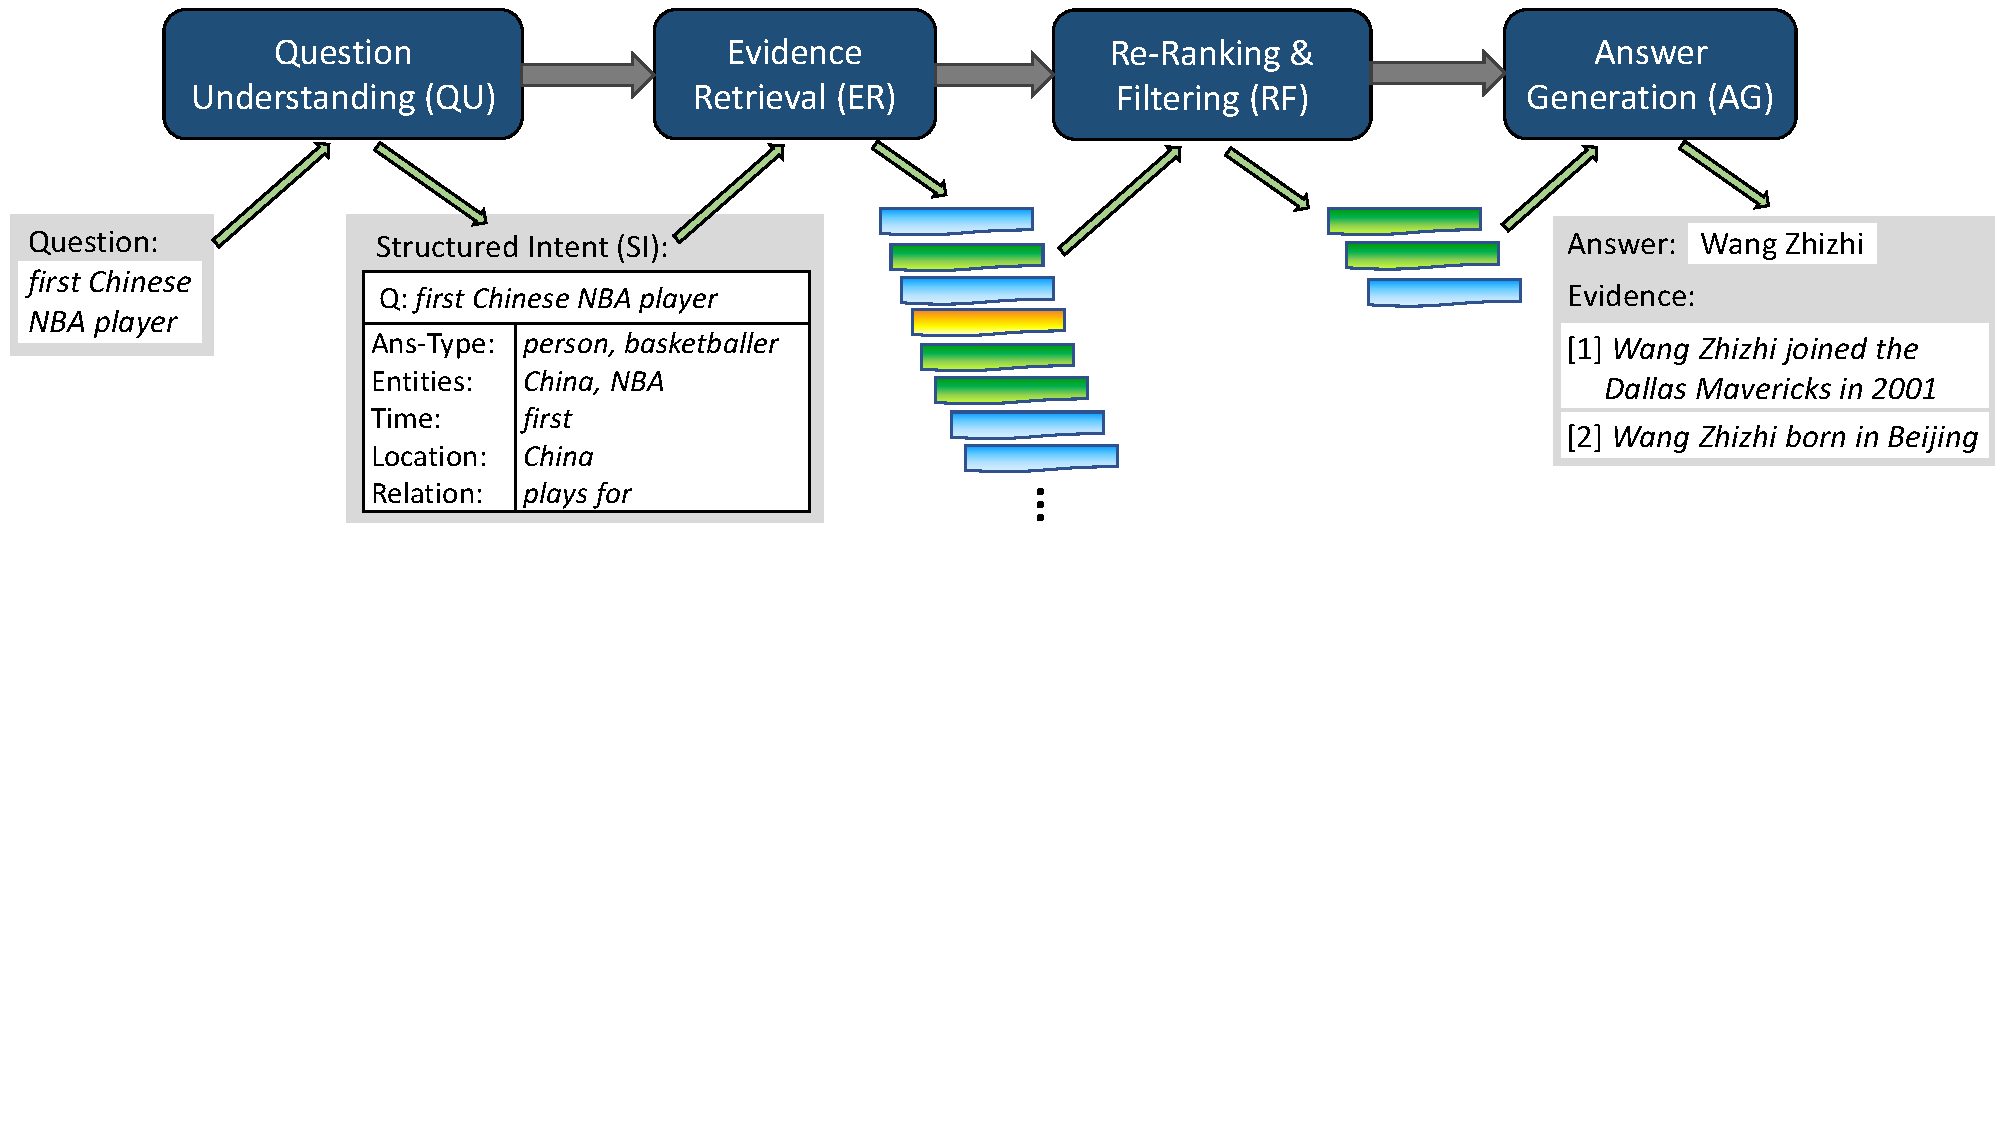
\includegraphics[width=\textwidth]{submissions/Gerhard2024/figures/compass-overview.pdf}
  \caption{Overview of the \method system.}
  \label{fig:compass-overview}
\end{figure}

% start with system overview
The \method system is a pipeline of four major stages, as illustrated in Figure \ref{fig:compass-overview}.
First, the input question is analyzed and decomposed, in order to compute a {\em structured intent (SI)} representation that will pass on to the subsequent steps, along with the original question. Second, the SI is utilized to retrieve pieces of evidence from different sources: text, KG and tables. 
Third, this pool of potentially useful evidence is filtered down, with iterative re-ranking, to arrive at a tractably small set of most promising evidence.
The final stage generates the answer from this evidence,
passing back the answer as well as evidence snippets for user-comprehensible explanation.

The second and fourth stage, Evidence Retrieval (ER) and Answer Generation (AG), are fairly standard. Such a two-phase architecture was called a retriever-reader architecture~\cite{Zhu-ODQA-survey:arxiv2021}. With a modern LLM replacing the earlier kinds of neural readers, this is the core of every RAG system~\cite{DBLP:journals/arXiv/abs-2312-10997}.

Stages 1 and 3 are unique elements of our architecture, judiciously introduced to improve both effectiveness (i.e., answer quality) and efficiency (i.e., computational cost).
Question Understanding (QU) provides the ER component with crisper and semantically refined input, and
the Re-Ranking \& Filtering (RF) stage is beneficial for
distilling the best evidence from the large pool of retrieved pieces.
The following subsections elaborate on the four stages of the pipeline, emphasizing the \method-specific steps QU and RF.



\subsection{Question Understanding (QU)}

% one par introducing the SI
To prepare the retrieval from different kinds of sources, including a KG, ad-hoc tables and text documents, it is useful to analyze and decompose the user question.
In this work, we aim to cast a question into a 
{\em structured intent (SI)} representation: essentially
a frame with faceted cues as slots, or equivalently, a concise set of key-value pairs. 
Figure \ref{fig:compass-overview} gives an idealized example for the question about the first Chinese NBA player. The facets or keys of potential interest here 
are:
\squishlist
\item {\em Ans-Type:} the expected answer type (or types when considering
different levels of semantic refinement), 
\item {\em Entities:} the salient entities in the question, and 
\item {\em Relation:} phrases that indicate which relation (between Q and A entities) the user is interested in. 
\squishend
\noindent In addition, as questions can have temporal or spatial aspects, the SI also foresees slots for:
\squishlist
\item {\em Time:} cues about answer-relevant time points or spans, including relative cues (e.g., ``before Covid'') and ordinal cues (e.g., ``first''), and
\item {\em Location:} cues about answer-relevant geo-locations.
\squishend

% discuss the spectrum of different SIs
\vspace{0.2cm}
\noindent The ideal SI for example question Q2 would look like:

\begin{quote}
{\em Ans-Type:} person, basketballer; {\em Entities:} China, NBA; {\em Time:} first;
{\em Location:} China; {\em Relation:} plays for.
\end{quote}

Note that the values for these slots can be crisp like entity names or dates, but they can also take the form of surface phrases. The SI purpose and value lie in the decomposition. In practice, many questions would only lead to a subset of faceted cues, leaving some slots empty. For the example in Figure \ref{fig:compass-overview}, an alternative SI could simply consist of

\begin{quote}
{\em Ans-Type:} person; {\em Entities:} China, NBA; {\em Time:} first.
\end{quote}

\noindent Even this simplified SI can be highly beneficial in guiding the subsequent evidence retrieval.

% sketch how an LM is trained to generate SIs 
To generate the SI from a user question, we employ a (small-scale) LM, specifically BART~\cite{DBLP:conf/acl/LewisLGGMLSZ20}, a Transformer-based auto-encoder with 140M parameters.\footnote{\url{https://huggingface.co/facebook/bart-base}}
BART is pre-trained for language representation; its power for our purpose comes from fine-tuning.
To this end, we generate (question, SI) pairs by using an instruction-trained LLM like GPT-4, with few-shot in-context learning (following our earlier work~\cite{Jia-FAITH:WWW2024}). 
Note that this is a one-time action; at inference-time we only use much smaller LMs.
The generated silver-standard pairs are then used to fine-tune BART.
In the experiments in this article, we leverage pre-existing collections of silver pairs, based on the training data of the CompMix benchmark~\cite{Christmann-CompMix:WWW2024}, 
comprising $3{,}400$ such pairs.


% outline value of SI for conversations
Although this paper focuses on single-shot questions, the \method architecture is also geared for conversational QA. In that setting, the SI can play an even bigger role, as (follow-up) questions are often formulated in a rather sloppy manner -- all but self-contained. For example, a conversation could start with a clear question {\em When did Wang Zhizhi join the NBA?}, followed a few dialog steps later, by a user utterance like {\em Which teams did he play for?} or simply {\em Which teams?}.
In such an informal conversation, the system needs to {\em contextualize} each user utterance based on the preceding turns in the dialog (e.g., inferring the relevant entities Wang Zhizhi and NBA from the conversational history).
For details on conversational QA, based on our architecture, see our earlier works~\cite{Christmann-CONVINSE:SIGIR2022,Christmann-Explaignn:SIGIR2023}.







%%%%%%%%%%%%%%%%%%%%%%%%%%%%%%%%%%%%%
\subsection{Evidence Retrieval (ER)}

The ER stage taps into a knowledge graph, a corpus of text documents, and a collection of web tables.
Specifically, for the experiments, we use the Wikidata KG,
all English Wikipedia articles, and all tables that are embedded in Wikipedia pages (incl. infoboxes, which can be seen as a special case of tables). 

% specifics: Clocq etc. - and the role of the SI
\vspace{0.2cm}
\noindent{\bf Retrieval from KG:}
To retrieve evidence from the KG, we utilize our earlier work
\clocq~\cite{Christmann-CLOCQ:WSDM2022}, which provides entity disambiguations and a relevant KG-subgraph for a given query.
Unlike most other works on QA-over-KG, \clocq fetches all KG-facts that are relevant for a given entity in a single step.
For example, when querying for
NBA players, it can traverse the KG neighborhood and pick up top teams, also considering so-called qualifier nodes in Wikidata which are often used for temporal scopes. 
As the disambiguation of entity names onto the KG can be tricky and noisy (e.g., China could be mapped to Chinese sports teams in all kinds of sports), \clocq considers several possible disambiguations~\cite{Christmann-CLOCQ:WSDM2022} (typically in the order of $10$ result entities).
The queries for \clocq are 
constructed by concatenating all slots of the question's SI.
For the example query about the first Chinese NBA player,
good result entities would be Dallas Mavericks, lists about NBA seasons, MVP awards etc., and their associated facts. These provide cues, but are likely insufficient to answer the question.


\vspace{0.2cm}
\noindent{\bf Retrieval from Text and Tables:}
The disambiguated entities returned by \clocq form anchors for tapping into text and tables.
\method first identifies 
relevant text documents and tables that refer to the anchor entities. With focus on Wikipedia, these are simply the articles for the respective entities. 
\method then constructs a keyword query that concatenates all available fields of the SI.
The query is evaluated against a linearized and verbalized representation (see below) of all sentences and all table rows in the selected documents.
This returns a set of sentences and 
and individual table rows, ranked by BM25 scores.


\vspace{0.2cm}
\noindent{\bf Evidence Verbalization:}
All results from the different data sources are uniformly treated by {\em linearizing} and {\em verbalizing} them
into token sequences. For KG results, the entity-centric triple sets are linearized via breadth-first traversal of the mini-graph starting from the entity node.
For tables, results are individual rows, which are contextualized by including labels from column headers and from the DOM-tree path of the article where the table comes from. For example, a table row about Wang Zhizhi playing for Dallas (Mavericks) in the 2000-2001 season, would be expressed as:

\vspace{0.05cm}
\hspace*{0.5cm} Wang Zhizhi / NBA Career / Season: 2000-2001, Team: Dallas, Games Played: 5 \dots
\vspace{0.05cm}

\noindent Finally, results from the text corpus are already in the form of token sequences, but we can additionally prefix these with the DOM-tree labels.
We can think of this entire pool of evidence as 
an on-the-fly corpus of potentially relevant pseudo-sentences, forming the input of the subsequent RF stage.


\vspace{0.2cm}
\noindent {\bf Result Ranking:}
Overall, the ER stage compiles a substantial set of evidence, possibly many thousands of entities, text snippets and table rows. Therefore, we practically restrict the pool to a subset of high-scoring pieces, like the top-$1000$.
For scoring, a simple BM25 model (a classical IR method) is applied. 
By default, we treat all evidence pieces uniformly with global scoring, no matter whether they come from KG, text or tables. 


\subsection{Re-Ranking and Filtering (RF)}

With a pool of top-$1000$ evidence pieces, we could invoke an LLM for answer generation. However, that would face a large fraction of noise (i.e., misleading evidence) and incur high costs of computation and energy consumption. 

For both of these reasons, we have devised light-weight techniques for iteratively reducing the top-$1000$ pieces to a small subset, say top-$30$ or top-$10$, that can be fed into an LLM at much lower cost (as LLM computations and pricing are at least linear in the number of input tokens). The difficulty is, of course, to do this without losing good evidence and reducing answer presence. Our techniques for this task are based on graph neural networks (GNNs)~\cite{Wu:IEEE2021} or cross-encoders (CEs)~\cite{Dejean:arxiv2024,Lin:MC2021}.

\myparagraph{GNN-based RF}
Given a large pool of evidence pieces from all sources, a bipartite graph is constructed:
\squishlist
\item {\em nodes} being evidence pieces or entities that occur in these pieces, and
\item {\em edges} connecting an evidence piece and an entity if the entity occurs in the evidence.
\squishend


The task for the GNN is to jointly score the evidence and the entity nodes in a multi-task learning setup. The latter are the {\em answer candidates}, and the evidence should give {\em faithful explanation} for an answer.
We build on our earlier work on explainable QA~\cite{Christmann-Explaignn:SIGIR2023}.

The node encodings are initialized with cross-encoder embeddings (see below) 
for node contents and the SI of the question. The inference iteratively adjusts the encodings based on message passing from neighboring nodes.
The GNN is trained via weak supervision from question-answer pairs:
evidence nodes are labeled as relevant if they are connected to
a gold answer.
More technical details are given in~\cite{Christmann-Explaignn:SIGIR2023}.

\method invokes the GNN in multiple rounds, iteratively reducing top-$k$ to top-$k^*$ nodes with $k^* \ll k$. In practice, we would typically consider two rounds: re-ranking top-$1000$ and pruning to top-100, and then reducing to top-30 or top-10, which are passed to the answer generation stage.
Note that this keeps the GNN at a tightly controlled size, so that its computational costs at inference-time are much smaller than those of an LLM.


\myparagraph{CE-based RF}
An alternative to the GNN inference is to employ a cross-encoder for scoring and re-ranking the evidence pieces.
These are transformers (typically with a small LM like BERT) that are fine-tuned for scoring the relatedness between a query and a document~\cite{Nogueira:arxiv2019}. In our case, the comparison is between the question SI and the evidence piece. In our experiments, we make use of two different cross-encoders, 
both trained on the MS-MARCO benchmark for passage retrieval~\cite{Bajaj:arxiv2018}, 
and fine-tuned on the respective benchmark (leveraging the same weak supervision data as for the GNNs),
the difference being in model size.\footnote{\url{https://huggingface.co/cross-encoder/ms-marco-MiniLM-L-4-v2} and\\ \url{https://huggingface.co/cross-encoder/ms-marco-MiniLM-L-6-v2}}
We use the smaller model to reduce top-$1000$ to top-100, and the larger model to go further down from top-100 to top-30.




%%%%%%%%%%%%%%%%%%%%%%%%%%%%%%%%%%%%%

\subsection{Answer Generation (AG)}

The last stage follows mainstream practice to invoke an LLM in a retrieval-augmented manner.
We call a `small-scale` LLM, specifically a fine-tuned LlaMA-3.1 model (8B-Instruct)\footnote{\url{https://huggingface.co/meta-llama/Llama-3.1-8B-Instruct}}, with a prompt \footnote{The specific prompt is \phrase{SI: \textless\texttt{concatenated SI}\textgreater \hspace{0.1cm} Evidence: \textless\texttt{evidence pieces}\textgreater}.}
consisting of:

\squishlist
\item the concatenated SI of the original question, and
\item the top-30 (or other top-$k^*$ with small $k^*$) evidence pieces.
\squishend

By the previous down-filtering of the original pool of evidence pieces, this last step has affordable cost in terms of computation time and energy consumption.

\vspace{0.2cm}
\noindent{\bf Fine-Tuning the LLM:}
We considered adding an instruction to the prompting, such as {\em ``answer this question solely based on the provided evidence snippets''}.
However, this turned out to be ineffective.
The reason why the model works well without such instructions is our task-specific fine-tuning.
We perform this by running the training data of benchmarks through the \method pipeline,
and training the AG stage with the top-30 evidence pieces as input.
Thus, the fine-tuning makes the model learn the role of evidence for RAG-based QA.

\vspace{0.2cm}
\noindent{\bf Explanations:}
The top-30 evidence pieces can be used to provide users with explanation of answers.
Optionally, these could be reduced further for comprehensibility.
Alternatively, we can fine-tune the LLM to provide both answers and concise explanations.
Since we can infer which evidences in the input mention the annotated ground-truth answers,
our method could be fine-tuned to provide such \textit{answering evidences} as well (cf.~\cite{Gao-citations:emnlp2023}).

\label{sec:exp}
\section{Experiments}


\label{setup}
\subsection{Experimental setup}


%%% BENCHMARKS
\myparagraphnospace{Benchmarks} We run experiments on three benchmarks with different characteristics of questions.

\squishlist
    \item \textbf{\compmix}.
    \compmix~\cite{Christmann-CompMix:WWW2024} is a benchmark which was specifically designed for evaluating QA systems operating over heterogeneous sources. The dataset has $9{,}410$ questions, out of which $2{,}764$ are used for testing.
    Answers are crisp entity names, dates, or other literals.
    
    \item \textbf{\crag}.
    We further evaluate on a subset of the \crag~\cite{Yang-CRAG} dataset, which was recently released as a testbed for RAG-based QA systems.
    We utilize the same pipeline and sources as outlined in Section~\ref{sec:method}, without using the web snippets or APIs provided with \crag. This way we focus on entity-centric questions that do not require access to live web data (e.g., news feeds), and disregard cases where the results would be up-to-date quantities.
    This restricts the test data to $436$ entity-centric questions, still enough for a proof of concept.
    
    \item \textbf{\timequestions}.
    To showcase the generalizability of our pipeline, we conduct experiments on~\timequestions~\cite{Jia-TimeQuestions},
    a benchmark for temporal QA. The dataset requires temporal understanding and reasoning, which are well-known limitations of
    LLMs~\cite{Dhingra-time-aware-LLM:TACL2022}. \timequestions has 16{,}181 questions (3{,}237 for testing).
\squishend

Typical examples for the questions in these three benchmarks are:

\begin{quote}
\compmix: \utterance{Which player won the most number of Man-of-the-Match titles in the FIFA world cup of 2006?}\\
 \indent \crag: \utterance{What was the worldwide box office sales for little hercules?}\\ 
  \indent \timequestions: \utterance{Which club did Cristiano Ronaldo play for before joining Real Madrid?}
\end{quote}

%%% BASELINES
\myparagraph{Baselines} As competitors or reference points to \method, we study the performance of the following methods:

\squishlist
    \item \textbf{Generative LLMs}.
    We compare \method against out-of-the-box LLMs: \textbf{\gptthree} (\texttt{text-davinci-003}), \textbf{\gptfour} (\texttt{gpt-4}) 
    and \textbf{\llama} (\texttt{meta-llama/Llama-3.1-8B-Instruct}).
    The same prompt is used for all LLMs, consistent with previous work~\cite{Christmann-CompMix:WWW2024, Zhang-Spaghetti:ACL2024}:
    \phrase{Please answer the following question by providing the crisp answer entity, date, year, or numeric number. Q: \textless\texttt{question}\textgreater}.
    

    \item \textbf{Heterogeneous QA methods}.
    \convinse~\cite{Christmann-CONVINSE:SIGIR2022}, \unikqa~\cite{Oguz-UniK-QA:NAACL2022}, \explaignn~\cite{Christmann-Explaignn:SIGIR2023}
    are QA methods designed to integrate heterogeneous sources: text, tables and KG. All of these  integrate the exact same sources as \method.

    
    \item \textbf{\textsc{State-of-the-art}}.
    For \compmix and \timequestions, we also compare against state-of-the-art methods from the literature: \spaghetti~\cite{Zhang-Spaghetti:ACL2024} and \textsc{Un-Faith}~\cite{Jia-FAITH:WWW2024}, which are among the best performing systems.
    
Results are taken from the literature whenever applicable.
On \crag, we use the models trained on \compmix for \method and heterogeneous QA baselines.
\squishend



%%% METRIC(S)
\myparagraph{Metrics}
We measure \textit{precision at 1} (\textbf{P@1}) as our main metric~\cite{RoyAnand:MC2021} on all benchmarks.
On \crag, we manually annotate answer correctness, as the ground-truth answer formats vary (e.g., entity name variants, lists, sentences).

We also compute the number of neural parameters aggregated over all sub-modules (\textbf{\#Parameters}).
Parameter counts for GPT-models are taken from~\cite{Minaee-LLM-survey}
(\gptfour might have less active parameters during inference).

For further analysis we measure \textit{answer presence} (\textbf{AP@k}),
i.e. whether the answer is present in the top-$k$ ranked evidence pieces,
and \textit{mean reciprocal rank} within the top-$k$ evidences (\textbf{MRR@k}).

%%% CONFIG
\myparagraph{Configuration}
Our implementation uses the \texttt{Llama3.1-8B-Instruct} model for the AG stage.
For the QU, ER and RF stages
we adopt code from the \explaignn project.\footnote{\url{https://explaignn.mpi-inf.mpg.de}}
For the ER stage, we use \clocq, setting its specific parameters to $k=10$ and $p=1{,}000$.

As default, we use the GNN technique for the RF stage.
For efficiency, we use light-weight models for initializing
the GNN encoders -- the same models used for the CE-based RF.\footnote{\url{https://huggingface.co/cross-encoder/ms-marco-MiniLM-L-4-v2} and\\\url{https://huggingface.co/cross-encoder/ms-marco-MiniLM-L-6-v2}}
The GNNs are trained for $5$ epochs with an epoch-wise evaluation strategy,
i.e. we choose the model with the best performance on the respective dev set.
We train the GNNs on graphs with a maximum of $100$ evidence and $400$ entity nodes (as scored by BM25).
During inference, the first GNN is applied on graphs with $1{,}000$ evidence and $4{,}000$ entity nodes, shrinking the pool of evidence pieces to the top-$100$.
The second GNN then runs on graphs with $100$ evidence and $400$ entity nodes.
The factor of 4 entities per evidence (on average) holds sufficient for the observed data,
and enables batched inference.
Other parameters are kept as is.

The AG model, based on \texttt{Llama3.1-8B-Instruct}, is 
fine-tuned
for $2$ epochs with a warm-up ratio of $0.01$ and a batch size of $8$, again with an epoch-wise evaluation strategy.
Other parameters are set to the default Hugging Face
training parameters.\footnote{\url{https://huggingface.co/docs/transformers/v4.46.2/en/main_classes/trainer\#transformers.TrainingArguments}}





\subsection{Main results}
%%% MAIN TABLE
\myparagraphnospace{\method is competitive on all benchmarks}
Main results of our experiments are shown in Table~\ref{tab:main-res}.
First of all, we note that \method achieves competitive performance across all three benchmarks.

On \compmix, baselines for heterogeneous QA and \llama perform similarly,
whereas GPT-based LLMs can answer more than $50$\% of the questions correctly.
\method exhibits substantially higher performance, on par with
the state-of-the-art method \textsc{Spaghetti}~\cite{Zhang-Spaghetti:ACL2024}
(which is based on \gptfour).

On the \crag dataset, P@1 drops for all methods except for \gptfour. 
The benchmark includes realistic questions,
which can be ambiguous/confusing (\phrase{who was the director for the report?}),
on ``exotic'' entities with answers in social media (\phrase{how many members does the teknoist have?}),
or require up-to-date information (\phrase{when did chris brown release a song or album the last time?}),
and other cases that are challenging for all methods.

Finally, \method establishes new state-of-the-art performance on the \timequestions benchmark.
Interestingly, all of the tested LLMs show greatly reduced performance on this benchmark,
which inherently requires temporal understanding and reasoning
-- a known weakness of stand-alone LLMs.


\begin{table} [h]
    \centering
    \newcolumntype{G}{>{\columncolor [gray] {0.90}}c}
    \begin{tabular}{l G G G c}
        \toprule
            \textbf{Method $\downarrow$ / Benchmark $\rightarrow$} & \textbf{\compmix}  & \textbf{\crag} & \textbf{\timequestions} & \textbf{\#Parameters} \\ 
        \midrule
            \textbf{\gptthree} 
            & $0.502$ &   $-$ & $0.224$ & $175{,}000$ M  \\
            % #params from https://arxiv.org/pdf/2402.06196

            \textbf{\gptfour}
            & $0.528$ &   $\mathbf{0.633}$ & $0.306$ & $1{,}760{,}000$ M \\
            % #params from https://arxiv.org/pdf/2402.06196

            \textbf{\llama~\cite{Touvron-LLaMA}} (8B-Instruct)
            & $0.431$ &   $0.385$ & $0.178$ & $8{,}030$ M  \\
            % #params from Huggingface (8,030,257,152)
        \midrule
            \textbf{\convinse~\cite{Christmann-CONVINSE:SIGIR2022}}
            & $0.407$  &   $0.298$ & $0.423$  & $362$ M \\
            % FiD: 222,903,936 + BART (SR-generation): 139,420,416 = 362,324,352 (python explaignn/question_understanding/structured_representation/get_num_params.py)

            \textbf{\unikqa~\cite{Oguz-UniK-QA:NAACL2022}}
            & $0.440$ &   $0.280$ & $0.424$ & $223$ M  \\
            % FiD: 222,903,936 (python explaignn/heterogeneous_answering/fid_module/FiD/get_num_params.py)
    
            \textbf{\explaignn~\cite{Christmann-Explaignn:SIGIR2023}} 
            & $0.442$ &   $0.303$ & $0.525$  & $328$ M \\
            % BART (SR-generation): 139,420,416 + 2GNNs: 94520832 + 93930240 = 327,871,488

        \midrule 
            \textbf{\textsc{State-of-the-art}}
            & $\mathbf{0.565}$ 
            & $-$
            & $0.571$  & $-$ \\

            & (\textsc{Spaghetti}~\cite{Zhang-Spaghetti:ACL2024})
            & 
            & (\textsc{Un-Faith}~\cite{Jia-FAITH:WWW2024}) &  \\

        \midrule
            \textbf{\method (ours)}
            & ${0.564}$ &   $0.362$ & $\mathbf{0.754}$  & $8{,}218$ M \\
            % BART (SR-generation): 139,420,416 + LLaMA: 8,030,257,152 + GNNs: 25,670,016 + 22,268,928 =  8,217,616,510
        \bottomrule
    \end{tabular} 
    \vspace*{-0.2cm}
    \caption{End-to-end P@1 of \method and baselines on three benchmarks. Results for \gptthree and \gptfour are taken from the literature~\cite{Christmann-CompMix:WWW2024, Jia-FAITH:WWW2024}. \gptthree is not accessible anymore, hence no results on \crag.
    }
    \label{tab:main-res}
\end{table}





%%% ANSWER SOURCES
\myparagraph{Integration of heterogeneous sources is vital}
\method integrates evidence from text, KG and tables into a unified framework.
We aim to better understand how this affects the answering performance of the method.
Table~\ref{tab:sources} shows end-to-end answering performance of \method
with different combinations of the input sources.
The results clearly indicate that all types of sources contribute, with option Text+KG+Tables performing best,
with a large margin over tapping only single source types.

\begin{table} [t] 
    \centering
    \newcolumntype{G}{>{\columncolor [gray] {0.90}}c}
    \newcolumntype{H}{>{\setbox0=\hbox\bgroup}c<{\egroup}@{}}
    	\begin{tabular}{l G G G H H H c c c} 
        \toprule
            \textbf{Benchmark $\rightarrow$}
                & \multicolumn{3}{G}{\textbf{\compmix}} 
                & \multicolumn{3}{H}{\textbf{\crag}}
                & \multicolumn{3}{c}{\textbf{\timequestions}} \\ 
        \midrule
            \textbf{Input sources $\downarrow$ / Metric $\rightarrow$}
                & \textbf{P@1} & \textbf{AP@100}  & \textbf{AP@30}
                & \textbf{P@1} & \textbf{AP@100}  & \textbf{AP@30}
                & \textbf{P@1} & \textbf{AP@100}  & \textbf{AP@30} \\
            \midrule
                \textbf{Text}           &  $0.455$  &  $0.563$  &  $0.531$ &  $?$  &  $?$  &  $?$ &  $0.539$  &  $0.515$  &  $0.487$   \\
                \textbf{KG}             &  $0.481$  &  $0.677$  &  $0.637$ &  $?$  &  $?$  &  $?$ &  $0.724$  &  $0.701$  &  $0.674$   \\
                \textbf{Tables}         &  $0.432$  &  $0.501$  &  $0.482$ &  $?$  &  $?$  &  $?$ &  $0.536$  &  $0.347$  &  $0.328$   \\
            \midrule
                \textbf{Text+KG}        &  $0.537$  &  $0.749$  &  $0.706$ &  $?$  &  $?$  &  $?$ &  $0.745$  &  $\mathbf{0.776}$  &  $0.748$   \\
                \textbf{Text+Tables}    &  $0.503$  &  $0.632$  &  $0.594$ &  $?$  &  $?$  &  $?$ &  $0.567$  &  $0.578$  &  $0.549$   \\
                \textbf{KG+Tables}      &  $0.524$  &  $0.728$  &  $0.692$ &  $?$  &  $?$  &  $?$ &  $ 0.743$  &  $0.731$  &  $0.703$   \\
            \midrule
                \textbf{Text+KG+Tables}    &  $\mathbf{0.564}$  &  $\mathbf{0.759}$  &  $\mathbf{0.724}$ &  $?$ &  $?$  &  $?$ & $\mathbf{0.754}$    & $\mathbf{0.776}$  &  $\mathbf{0.749}$   \\
            \bottomrule
    \end{tabular}
    \vspace*{-0.2cm}
    \caption{Answer presence and answering precision of \method with different combinations of input sources (on the respective test sets).}
    \label{tab:sources}
\end{table}




\subsection{Analysis}

%%% TOP-K vs. 3xTOP-(K/3)
\myparagraph{Unified retrieval enhances performance}
In the RF stage, we re-rank and filter evidence from different source types,
and feed the unified top-\textit{k}* into the AG stage.
We conduct a comparison in which we consider
the top-$10$ evidence pieces from each source type individually. This gives equal influence to KG, text and tables, whereas our default is based on global ranking.
Table~\ref{tab:unified-retrieval} shows the results for this analysis, showing our default choice performs better.
The reason is that different questions require different amounts of evidence from each of the source types.

\begin{table} [t] 
    \centering
    \newcolumntype{G}{>{\columncolor [gray] {0.90}}c}
    \newcolumntype{H}{>{\setbox0=\hbox\bgroup}c<{\egroup}@{}}
    	\begin{tabular}{l G G H H} 
        \toprule
            \textbf{Input evidences $\downarrow$ / Metric $\rightarrow$} & \textbf{P@1} & \textbf{AP@30}  & \textbf{\crag} & \textbf{\timequestions} \\ 
            \midrule
                \textbf{Top-30 Text+KG+Tables (ours)}             &  $\mathbf{0.574}$  &  $\mathbf{0.710}$  &  $-$  &  $-$   \\
                \textbf{Top-10 Text + Top-10 KG + Top-10 Tables}        &  $0.560$    &  $0.709$  &  $-$  &  $-$   \\
            \bottomrule
    \end{tabular}
    \vspace*{-0.2cm}
    \caption{Answer presence and precision
    of \method for different choices of top-30 
    (on \compmix dev set).}
    \label{tab:unified-retrieval}
\end{table}


%%% NUMBER OF EVIDENCES
\myparagraph{\method works well with small amounts of evidence}
We investigate the 
influence of 
the number of evidence pieces
fed into the AG stage, varying it from $5$ to $100$.
Results are shown in Figure~\ref{fig:res-num-evidences}.
As the curve shows, there is a sharp increase in precision as we add evidence up to 30 or 40 pieces, which is around our default of top-30. This indicates that a certain amount of evidence is needed, to overcome the inherent noise and arrive at sufficient answer presence. 
As we increase the amount of evidence further, we observe a saturation effect, and eventually a degration of performance. Too much evidence not only has diminishing returns, but can actually be confusing for the AG stage. This reconfirms our heuristic choice of top-30: enough for good answering while keeping computational costs reasonably low.


\begin{figure}[t]
    \centering
    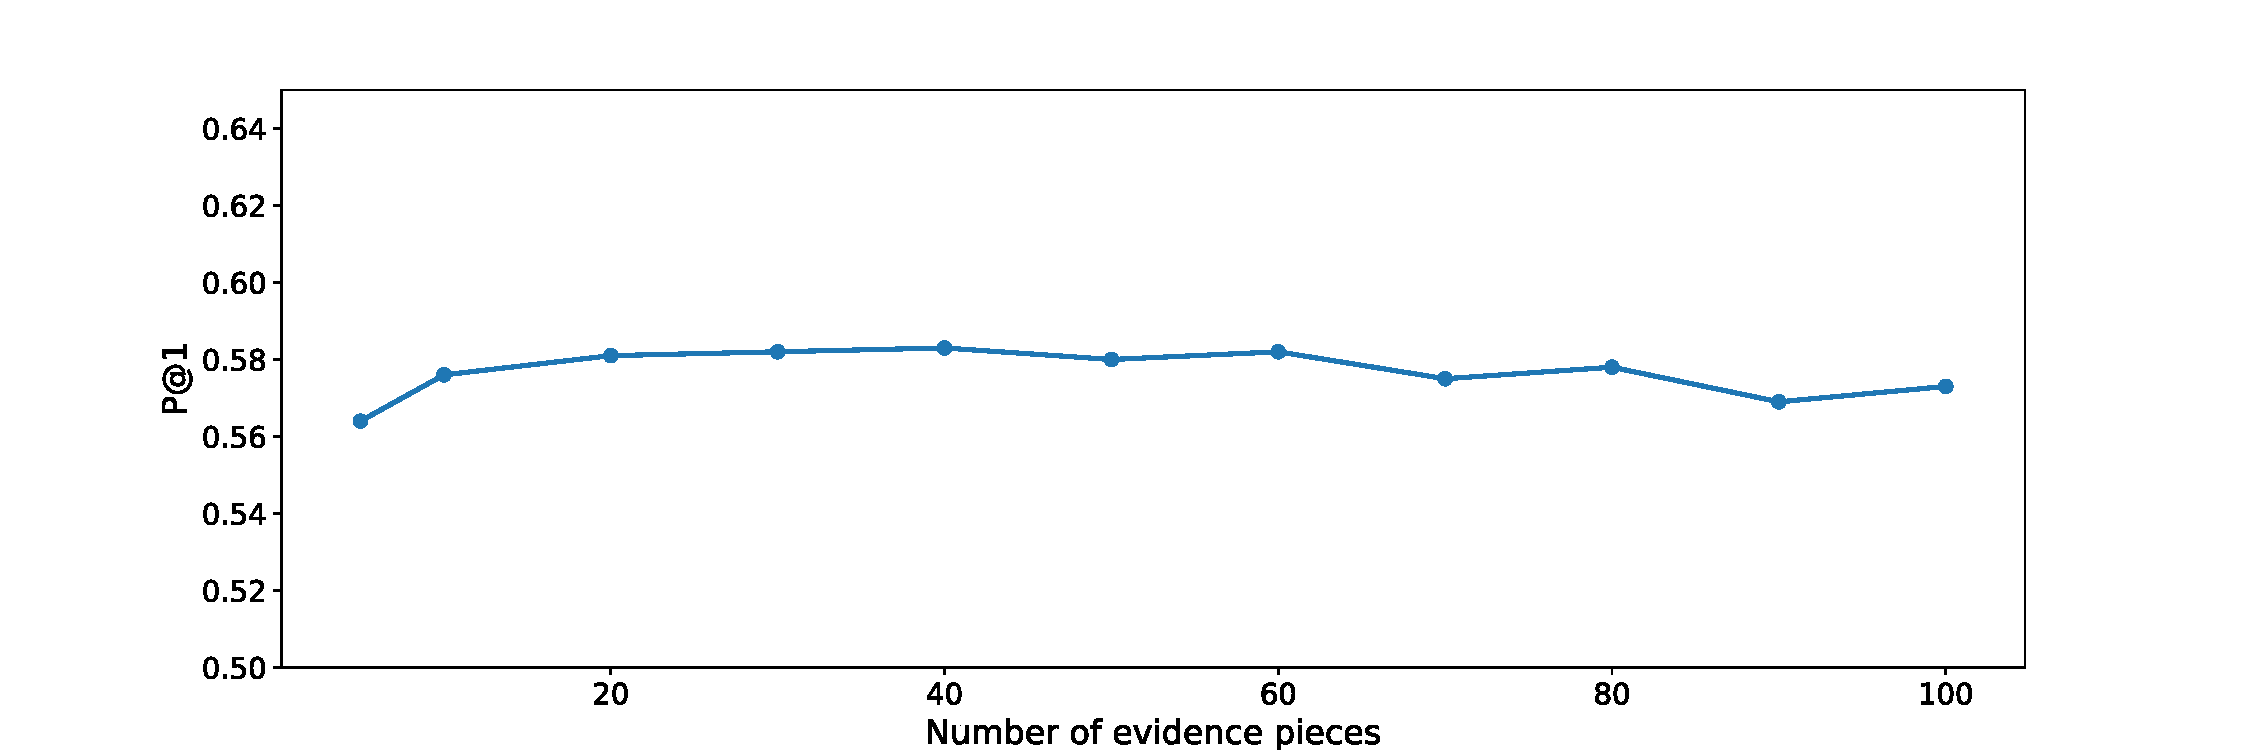
\includegraphics[width=0.8\textwidth]{submissions/Gerhard2024/figures/p_at_1-line_with_evidences.pdf}
    \vspace*{-0.2cm}
    \caption{Performance of \method on the \compmix dev set with different numbers of evidence.}
    \label{fig:res-num-evidences}
    \vspace*{-0.2cm}
\end{figure}



%%% ABLATION
\myparagraph{Ablation study on re-ranking} For more insight on the possible configurations of the RF stage, we conducted an ablation study with different options, including solely relying on the initial BM25 scoring without explicit re-ranking. The results are shown in Table \ref{tab:ablation2}. We observe that the iterative reduction in two steps is slightly better than the single-step variants (going down from top-1000 to top-30 in one RF step). Between the two options of using a GNN or a CE, the differences are negligible. A notable effect is that our RF techniques retain the answer presence at a very high level, only a bit lower than for the initial top-1000. 
The last two rows of Table \ref{tab:ablation2} demonstrate that RF is crucial: without explicit re-ranking, the technique of just picking smaller top-$k$ from the original BM25 model leads to substantial degradation in both answer presence and precision. 


\begin{table} [t] \small
    \centering
    \newcolumntype{G}{>{\columncolor [gray] {0.90}}c}
    \newcolumntype{H}{>{\setbox0=\hbox\bgroup}c<{\egroup}@{}}
    	\begin{tabular}{l G H G G G} 
        \toprule
            & \multicolumn{5}{G}{\textbf{\compmix} (dev set)} \\
        \midrule
            \textbf{RF Method $\downarrow$ / Metric $\rightarrow$} & \textbf{P@1} & \textbf{AP@1000} & \textbf{AP@100}  & \textbf{AP@30} & \textbf{MRR@100} \\ 
        \midrule
            \textbf{GNN: 1000 $\rightarrow$ 100 $\rightarrow$ 30}             &  $\mathbf{0.574}$  & $0.760$ &  $0.738$  &  $0.710$  &  $\mathbf{0.572}$  \\
            \textbf{CE: 1000 $\rightarrow$ 100 $\rightarrow$ 30}          &  $0.573$  & $0.760$  &   $\mathbf{0.740}$ &  $\mathbf{0.721}$   &  $0.553$   \\
        \midrule
            \textbf{GNN: 1000 $\rightarrow$ 30} &  $0.567$  & $?$  &   $n/a$ &  $0.710$   &  $0.567$   \\
         \textbf{CE: 1000 $\rightarrow$ 30} &  $0.570$  & $0.760$  &   $n/a$ &  $0.715$   &  $0.558$   \\
            \midrule
           \textbf{BM25: 100 (w/o GNN or CE)} &  $0.490$ & $0.760$  &  $0.652$  &  $n/a$  &  $0.259$ \\       
            \textbf{BM25: 30 (w/o GNN or CE)} &  $0.468$  & $0.760$  &  $n/a$ &  $0.534$   &  $0.259$   \\
            \bottomrule
    \end{tabular}
    \vspace*{-0.2cm}
    \caption{Ablation study for different RF strategies of \method on the \compmix dev set. The answer presence in the RF input with top-$1000$ evidence pieces is $0.760$.}
    \label{tab:ablation2}
\end{table}



\myparagraph{Quality of SI}
To assess the quality and robustness of the Structured Intents, we
inspected a sample of questions and their SIs.
Table~\ref{tab:question-SI-examples} gives three anecdotic examples.
We show SIs generated by \method, which makes use of the pre-existing collection from the \compmix benchmark for training.
This training data was obtained via different heuristics, 
which can be a limiting factor when user intents become more complex.

Therefore, we also looked at SIs derived via in-context learning (ICL) using \gptfour with $5$ handcrafted examples.
As shown in our earlier work on temporal QA~\cite{Jia-FAITH:WWW2024},
such data can be used for training smaller models (e.g., BART),
which can greatly boost the completeness and overall quality of the generated SIs.

From the sampled set, we observed that the ICL-based SIs are more
complete with all slots filled, whereas the BART-based SIs focused more
on the main slots Answer-type, Entities and Relation.
However, both approaches achieve very high quality in filling the slots,
capturing the user's information need very well.

Interestingly, when questions get complicated, with nested phrases, 
the ICL-based variant succeeds in decomposing the questions, based on only $5$ ICL examples.
For example, for the question {\em ``which German state had the most Corona-related death cases in the first year after the outbreak?''}
the Time slot becomes {\em ``first year after Corona outbreak''},
which can be resolved to identify the temporal scope.
In general, we believe that such question decomposition, beyond simple temporal constraints,
would be an interesting theme for future work.

\begin{table} [t] 
    \centering
    \small
    \newcolumntype{G}{>{\columncolor [gray] {0.90}}c}
    \newcolumntype{H}{>{\setbox0=\hbox\bgroup}c<{\egroup}@{}}
    \resizebox*{\textwidth}{!}{
        \begin{tabular}{p{6cm}|p{6cm}|p{6cm}} 
        \toprule
            \textbf{Question} & \textbf{Current SI by \method} & \textbf{SI via ICL} \\
        \midrule
        \textit{what was disneys first color movie?}
            & Ans-Type: \textit{animated feature film} & Ans-Type: \textit{film, animated film} \\
            & Entities: \textit{disneys} & Entities: \textit{Disney} \\
            & Relation: \textit{was first color movie} & Relation: \textit{first color movie} \\
            &  & Time: \textit{first} \\
        \midrule
        \textit{at the oscars, who won best actor in 2018?}
            & Ans-Type: \textit{human} & Ans-Type: \textit{person, actor} \\
            & Entities: \textit{at the oscars} & Entities: \textit{Oscars, 2018} \\
            & Relation: \textit{who won best actor in 2018} & Relation: \textit{won best actor} \\
            &  & Time: \textit{2018} \\
        \midrule
        \textit{which German state had the most Corona-} & Ans-Type: \textit{state} & Ans-Type: \textit{location, state} \\
        \textit{related death cases in the first year after} & Entities: \textit{Germany, Corona} & Entities: \textit{Germany, Corona-related deaths} \\
        \textit{the outbreak?} & Relation: \textit{which state had the most related} & Relation: \textit{highest count of death cases} \\
        & \textit{death cases in the first year after the out-}  & Location: \textit{Germany} \\
            & \textit{break}  & Time: \textit{first year after Corona outbreak} \\
        \bottomrule
    \end{tabular}
    }
    \vspace*{-0.2cm}
    \caption{Examples for pairs of question and generated SI.}
    \label{tab:question-SI-examples}
\end{table}




%%% REFRAIN FROM ANSWER
\myparagraph{Refraining from answering}
%%% Searched for: "generated_answer I" (with I being the full word, not partial) in the generated answers of LLaMA
%%% yields 245 results out of 2764 questions on CompMix
%%% yields 1270 results out of 3237 questions on TimeQuestions
We can train our model to refrain from answering in scenarios
where the provided evidence does not contain an answer to the question.
Specifically, during training, when the answer is not present in the evidence,
we change the target answer to {\em unknown}. This variant is referred to as \method {\em (faithful)}.

We measure the ratio of questions for which {\em unknown} is provided as answer,
and the P@1 restricted to questions that are answered.
The accuracy of refraining from answering is measured as well,
based on whether the answer is present in the evidence or not.
We conduct this experiment on \compmix and \timequestions,
for which we can compute answer presence exactly.
We also compute results for \llama, which is already instructed 
with the option to answer ``don't know''.
Table~\ref{tab:refrain-from-answer} shows the results.
For \compmix, we observe that \method has high accuracy on refraining when appropriate,
whereas \llama tends to be overconfident with a very small rate of {\em unknowns}, leading to incorrect answers.

\begin{table} [t] \small
    \centering
    \newcolumntype{G}{>{\columncolor [gray] {0.90}}c}
    \newcolumntype{H}{>{\setbox0=\hbox\bgroup}c<{\egroup}@{}}
    	\begin{tabular}{l G G G G c c c c} 
        \toprule
            & \multicolumn{4}{G}{\textbf{\compmix}} & \multicolumn{4}{c}{\textbf{\timequestions}} \\
            \midrule
            \textbf{Metric $\rightarrow$} & \textbf{P@1}  & \textbf{P@1} & \textbf{Refrain} & \textbf{Refrain} & \textbf{P@1}  & \textbf{P@1} & \textbf{Refrain} & \textbf{Refrain} \\ 
            \textbf{Method $\downarrow$} &                 & \textbf{(answered)} & \textbf{rate} & \textbf{accuracy} &                 & \textbf{(answered)} & \textbf{rate} & \textbf{accuracy} \\ 
            \midrule
                \textbf{\llama}             &  $0.431$  &  $0.471$  &  $0.089$  &  $n/a$  &  $0.177$  &  $0.276$  &  $0.392$  &  $n/a$  \\
                \textbf{\method (faithful)}           &  $0.497$  &  $0.713$  &  $0.303$  &  $0.838$ &  $0.597$  &  $0.804$  &  $0.257$  &  $0.864$  \\
            \bottomrule
    \end{tabular}
    \vspace*{-0.2cm}
    \caption{
        Performance of \method with option to refrain from answering (``don't know'').
    }
    \label{tab:refrain-from-answer}
\end{table}

\label{sec:disc}
\section{Insights, Limitations, and Challenges}


\noindent{\bf Benchmark Performance.} Our method, RAG-based \method with an 8B LLaMA model, outperforms much larger LLMs like \gptfour on two of the three benchmarks, with a very large margin for temporal questions. Obviously, pre-trained LLMs have only limited sense of properly positioning ``remembered’’ facts on the timeline even with training data that exceeds ours by several orders of magnitude. This confirms our intuition that LLMs alone are not good at ``recalling’’  higher-arity relations that require combining distant pieces of evidence. This is a sweet spot for RAG. Only for 
the \crag benchmark, \method is substantially inferior to a full-blown LLM. This is likely due to the nature of the questions: not necessarily the complexity of the information needs, but the need for more web sources (beyond what our experiments tap into).

\vspace{0.2cm}
\noindent{\bf Cost/Performance Ratio.} The most important take-away from our experiments is that \method achieves its competitive performance at a much lower cost than the full LLMs. Assuming that the consumed GFlops are proportional to the number of model parameters, \method achieves a cost reduction by a factor of 200x for \gptthree and 2000x for \gptfour. This does not only mean less computation, but also a massively lower electricity bill and climate impact.  

\vspace{0.2cm}
\noindent{\bf Role of Question Understanding.} We did not systematically investigate the influence of the Structured Intent in the \method pipeline. However, the comparison to the big GPT models reflects the role of the SI, as we prompt the GPT models in their natural mode with the original questions. The linearized sequence of available SI slots does not always have major advantages, but there are enough cases where specific facets provide crucial cues. This holds especially for the Entities slot, as this drives the gathering of evidence in the ER stage (cf.~\cite{Christmann-CONVINSE:SIGIR2022}, and for the Time slot, as these cues are often decisive for temporal questions (cf.~\cite{Jia-FAITH:WWW2024}).

\vspace{0.2cm}
\noindent{\bf Role of Re-Ranking.} As our ablation studies show, merely using top-$k$ evidence from an initial BM25-style ranking does not provide good performance. Also, there seems to be sweet spot in the choice of $k$: we need enough evidence for connecting the dots if the question requires multiple pieces of information, or for corroborating candidates if the question finds many useful but noisy pieces. In the experiments, $k=30$ turns out to be good choice; much lower $k$ results in insufficient evidence, and much larger $k$ leads to saturation and ultimately degrading performance. Our argument for iteratively shrinking the candidate set in multiple rounds of re-ranking is substantiated in our experiments, but the gain of doing this, compared to GNN- or CE-based re-ranking from 1000 to 30, is not big. More research is called to better understand the role of ranking in RAG. 

\vspace{0.2cm}
\noindent{\bf Limitations of Evidence Retrieval.}
For ER, we adopted more or less standard techniques. The results showed very good answer presence, in the order of 75\% in the top-100 or even top-30. An important case where this is insufficient are questions that require aggregating information over a large number of evidence pieces. An example is asking for the life-time total of 3-point scores of the basketball player Dirk Nowitzki.
This requires collecting a set of per-season tables with NBA player statistics, but also other web sources with numbers for his career before he joined the NBA (including his youth teams).
Of course, there are sometimes shortcuts like a Wikipedia article or biography mentioning the total number, but this cannot be universally assumed. The bottom line is that ER should be reconsidered as well, striving to improve the recall dimension.

\vspace{0.2cm}
\noindent{\bf Limitations of Answer Generation.}
For AG, we simply rely on a LLM,
using it as an extractor (``reader'') from the given evidence. Despite the wide belief that LLMs can perform deep
reasoning over many pieces of evidence, our experience is that the extraction works only well – robustly and faithfully – for relatively simple questions with a few multi-hop joins or simple aggregation over a few pieces. However, complicated questions such as asking for the top-100 NBA players with the largest number of life-time 3-point scores (again including their pre-NBA careers) are currently out of scope and will likely remain so for quite some time. This offers many opportunities for pushing the envelope further.

\vspace{0.2cm}
\noindent{\bf Trust in Data Sources.}
In our experiments, we considered all heterogeneous sources as trustworthy and unbiased. With focus on Wikidata and Wikipedia, this assumption has been well justified. In the wild, however, input data for RAG-based systems likely exhibit a wide spectrum of quality issues, in terms of stale information, biased positions, or simply false statements. Identifying trustworthy and up-to-date evidence and dealing with conflicting data, has been explored in other contexts (e.g., for KG curation~\cite{Dong-Trust:PVLDB2015}), but remains a major challenge for RAG-based QA.


\vspace{0.2cm}
\noindent{\bf Open Challenges and Future Work.} The best-performing methods in our experiment, mostly \method, reach P@1 values of 56\% for \compmix and 75\% for \timequestions. 
For the latter, the answer presence in the top-100 is only slightly higher; so the AG stage hardly misses anything.
However, for \compmix, the answer presence is 75\% -- much higher than what our system can actually answer. Obviously, closing this gap is a major direction to pursue, with focus on the RF and AG stages. However, missing one fourth of the answers completely in the top-100 pool, is a big problem as well. This requires improving recall at the ER stage, possibly with better guidance by the QU, which in turn needs more sources beyond the scope of our experiments (currently limited to Wikidata and Wikipedia). 

In general, we need to think beyond this kind of ``benchmark mindset’’. Even if we reached 80\% or 90\% precision and recall, we would still have a substantial fraction of questions that are answered incorrectly
or not at all. 
The remaining errors may not be a problem for chatbots, but they would be a showstopper for the deployment of mission-critical applications in business or science. We believe that this big gap is a shortcoming of {\em all methods}, not an issue that comes from the data alone. For trivia-style QA, as looked at in this paper, a smart human in ``open book’’ mode and no time limitation should be able to properly answer practically all questions, just by reading pieces of web contents and putting things together. Neither LLMs nor state-of-the-art RAG are the final solution; substantial research and creative ideas are needed to further advance QA.


\clearpage
\newpage

\newcommand{\bibauthors}[1]{{#1}}
\newcommand{\bibtitle}[1]{\emph{#1}}
\newcommand{\bibconf}[1]{{#1}}

\begin{thebibliography}{10}

\bibitem{Bajaj:arxiv2018}
\bibauthors{Payal Bajaj, Daniel Campos, Nick Craswell, Li Deng, Jianfeng Gao, Xiaodong Liu, Rangan Majumder, Andrew McNamara, Bhaskar Mitra, Tri Nguyen, Mir Rosenberg, Xia Song, Alina Stoica, Saurabh Tiwary, Tong Wang.}
\bibtitle{MS MARCO: A Human Generated MAchine Reading COmprehension Dataset.}
In \bibconf{arXiv 2018}.

\bibitem{DBLP:conf/acl/ChenFWB17}
\bibauthors{Danqi Chen, Adam Fisch, Jason Weston and Antoine Bordes.}
\bibtitle{Reading Wikipedia to Answer Open-Domain Questions.}
In \bibconf{ACL 2017}.

\bibitem{Christmann-CONVINSE:SIGIR2022}
\bibauthors{Philipp Christmann, Rishiraj Saha Roy, Gerhard Weikum.}
\bibtitle{Conversational Question Answering on Heterogeneous Sources.}
In \bibconf{SIGIR 2022}.

\bibitem{Christmann-CLOCQ:WSDM2022}
\bibauthors{Philipp Christmann, Rishiraj Saha Roy, Gerhard Weikum.}
\bibtitle{Beyond NED: Fast and Effective Search Space Reduction for Complex Question Answering over Knowledge Bases.}
In \bibconf{WSDM 2022}.

\bibitem{Christmann-Explaignn:SIGIR2023}
\bibauthors{Philipp Christmann, Rishiraj Saha Roy, Gerhard Weikum.}
\bibtitle{Explainable Conversational Question Answering over Heterogeneous Sources via Iterative Graph Neural Networks.}
In \bibconf{SIGIR 2023}.

\bibitem{Christmann-CompMix:WWW2024}
\bibauthors{Philipp Christmann, Rishiraj Saha Roy, Gerhard Weikum.}
\bibtitle{CompMix: A Benchmark for Heterogeneous Question Answering.}
In \bibconf{WWW 2024}.

\bibitem{Dejean:arxiv2024}
\bibauthors{Herve Dejean, Stephane Clinchant, Thibault Formal.}
\bibtitle{A Thorough Comparison of Cross-Encoders and LLMs for Reranking SPLADE.}
In \bibconf{arXiv 2024}.

\bibitem{Dhingra-time-aware-LLM:TACL2022}
\bibauthors{Bhuwan Dhingra, Jeremy R Cole, Julian Martin Eisenschlos, Daniel Gillick, Jacob Eisenstein, and William W Cohen.}
\bibtitle{Time-Aware Language Models as Temporal Knowledge Bases.}
In \bibconf{TACL 2022}.

\bibitem{Dong-Trust:PVLDB2015}
\bibauthors{Xin Luna Dong, Evgeniy Gabrilovich, Kevin Murphy, Van Dang, Wilko Horn, Camillo Lugaresi, Shaohua Sun, Wei Zhang.}
\bibtitle{Knowledge-Based Trust: Estimating the Trustworthiness of Web Sources.}
In \bibconf{PVLDB 2015}.

\bibitem{DBLP:journals/arXiv/abs-2312-10997}
\bibauthors{Yunfan Gao, Yun Xiong, Xinyu Gao, Kangxiang Jia, Jinliu Pan, Yuxi Bi, Yi Dai, Jiawei Sun, Qianyu Guo, Meng Wang, Haofen Wang.}
\bibtitle{Retrieval-Augmented Generation for Large Language Models: A Survey.}
In \bibconf{arXiv 2023}.

\bibitem{Gao-citations:emnlp2023}
\bibauthors{Tianyu Gao, Howard Yen, Jiatong Yu, Danqi Chen.}
\bibtitle{Enabling Large Language Models to Generate Text with Citations.}
In \bibconf{EMNLP 2023}.

\bibitem{Guu-REALM:ICML2020}
\bibauthors{Kelvin Guu, Kenton Lee, Zora Tung, Panupong Pasupat, Ming-Wei Chang.}
\bibtitle{Retrieval Augmented Language Model Pre-Training.}
In \bibconf{ICML 2020}.

\bibitem{DBLP:conf/eacl/IzacardG21}
\bibauthors{Gautier Izacard, Edouard Grave.}
\bibtitle{Leveraging Passage Retrieval with Generative Models for Open Domain Question Answering.}
In \bibconf{EACL 2021}.

\bibitem{Jia-TimeQuestions}
\bibauthors{Zhen Jia, Soumajit Pramanik, Rishiraj Saha Roy, and Gerhard Weikum.}
\bibtitle{Complex Temporal Question Answering on Knowledge Graphs.}
In \bibconf{CIKM 2021}.

\bibitem{Jia-FAITH:WWW2024}
\bibauthors{Zhen Jia, Philipp Christmann, Gerhard Weikum.}
\bibtitle{Faithful Temporal Question Answering over Heterogeneous Sources.}
In \bibconf{WWW 2024}.

\bibitem{DBLP:journals/arXiv/abs-2305-06984}
\bibauthors{Ehsan Kamalloo, Nouha Dziri, Charles L. A. Clarke, Davood Rafiei.}
\bibtitle{Evaluating Open-Domain Question Answering in the Era of Large Language Models.}
In \bibconf{arXiv 2023}.

\bibitem{Kandpal:ICML2023}
\bibauthors{Nikhil Kandpal, Haikang Deng, Adam Roberts, Eric Wallace, Colin Raffel.}
\bibtitle{Large Language Models Struggle to Learn Long-Tail Knowledge.}
In \bibconf{ICML 2023}.

\bibitem{DBLP:conf/emnlp/KarpukhinOMLWEC20}
\bibauthors{Vladimir Karpukhin, Barlas Oguz, Sewon Min, Patrick S. H. Lewis, Ledell Wu, Sergey Edunov, Danqi Chen, Wen-tau Yih.}
\bibtitle{Dense Passage Retrieval for Open-Domain Question Answering.}
In \bibconf{EMNLP 2020}.

\bibitem{Lee-MATTER:ACL2024}
\bibauthors{Dongkyu Lee, Chandana Satya Prakash, Jack FitzGerald, Jens Lehmann.}
\bibtitle{MATTER: Memory-Augmented Transformer Using Heterogeneous Knowledge Sources.}
In \bibconf{ACL 2024}.

\bibitem{DBLP:conf/acl/LewisLGGMLSZ20}
\bibauthors{Mike Lewis, Yinhan Liu, Naman Goyal, Marjan Ghazvininejad, Abdelrahman Mohamed, Omer Levy, Veselin Stoyanov, Luke Zettlemoyer.}
\bibtitle{BART: Denoising Sequence-to-Sequence Pre-training for Natural Language Generation, Translation, and Comprehension.}
In \bibconf{ACL 2020}.

\bibitem{DBLP:conf/nips/LewisPPPKGKLYR020}
\bibauthors{Patrick S. H. Lewis, Ethan Perez, Aleksandra Piktus, Fabio Petroni, Vladimir Karpukhin, Naman Goyal, Heinrich Küttler, Mike Lewis, Wen-tau Yih, Tim Rocktäschel, Sebastian Riedel, Douwe Kiela.}
\bibtitle{Retrieval-Augmented Generation for Knowledge-Intensive NLP Tasks.}
In \bibconf{NeurIPS 2020}.

\bibitem{Lin:MC2021}
\bibauthors{Jimmy Lin, Rodrigo Frassetto Nogueira, Andrew Yates.}
\bibtitle{Pretrained Transformers for Text Ranking: BERT and Beyond.}
In \bibconf{Morgan \& Claypool Publishers 2021}.

\bibitem{Liu-SUQL:NAACL2024}
\bibauthors{Shicheng Liu, Jialiang Xu, Wesley Tjangnaka, Sina J. Semnani, Chen Jie Yu, Monica Lam.}
\bibtitle{SUQL: Conversational Search over Structured and Unstructured Data with Large Language Models.}
In \bibconf{NAACL-HLT 2024}.

\bibitem{Mavi:FnT2024}
\bibauthors{Vaibhav Mavi, Anubhav Jangra, Adam Jatowt.}
\bibtitle{Multi-hop Question Answering.}
In \bibconf{Foundations and Trends in Information Retrieval 2024}.

\bibitem{Minaee-LLM-survey}
\bibauthors{Shervin Minaee, Tomas Mikolov, Narjes Nikzad, Meysam Chenaghlu, Richard}
\bibtitle{Socher, Xavier Amatriain, and Jianfeng Gao.}
Large Language Models: A Survey.
In \bibconf{arXiv 2024}.

\bibitem{Nogueira:arxiv2019}
\bibauthors{Rodrigo Frassetto Nogueira, Kyunghyun Cho.}
\bibtitle{Passage Re-ranking with BERT.}
In \bibconf{arXiv 2019}.

\bibitem{Oguz-UniK-QA:NAACL2022}
\bibauthors{Barlas Oguz, Xilun Chen, Vladimir Karpukhin, Stan Peshterliev, Dmytro Okhonko, Michael Sejr Schlichtkrull, Sonal Gupta, Yashar Mehdad, Scott Yih.}
\bibtitle{UniK-QA: Unified Representations of Structured and Unstructured Knowledge for Open-Domain Question Answering.}
In \bibconf{NAACL-HLT 2022}.

\bibitem{RogersGA:CS2023}
\bibauthors{Anna Rogers, Matt Gardner, Isabelle Augenstein.}
\bibtitle{QA Dataset Explosion: A Taxonomy of NLP Resources for Question Answering and Reading Comprehension.}
In \bibconf{ACM Computing Surveys 2023}.

\bibitem{RoyAnand:MC2021}
\bibauthors{Rishiraj Saha Roy, Avishek Anand.}
\bibtitle{Question Answering for the Curated Web: Tasks and Methods in QA over Knowledge Bases and Text Collections.}
In \bibconf{Synthesis Lectures on Information Concepts, Retrieval, and Services, Morgan \& Claypool Publishers 2021}.

\bibitem{Pramanik-Uniqorn:JWS2024}
\bibauthors{Soumajit Pramanik, Jesujoba Alabi, Rishiraj Saha Roy, Gerhard Weikum.}
\bibtitle{UNIQORN: Unified Question Answering over RDF Knowledge Graphs and Natural Language Text.}
In \bibconf{Journal of Web Semantics 2024}.

\bibitem{Sun-PullNet:EMNLP2019}
\bibauthors{Haitian Sun, Tania Bedrax-Weiss, William W. Cohen.}
\bibtitle{PullNet: Open Domain Question Answering with Iterative Retrieval on Knowledge Bases and Text.}
In \bibconf{EMNLP/IJCNLP 2019}.

\bibitem{Sun:NAACL2024}
\bibauthors{Kai Sun, Yifan Ethan Xu, Hanwen Zha, Yue Liu, Xin Luna Dong.}
\bibtitle{Head-to-Tail: How Knowledgeable are Large Language Models (LLMs)? A.K.A. Will LLMs Replace Knowledge Graphs?}
In \bibconf{NAACL-HLT 2024}.

\bibitem{Touvron-LLaMA}
\bibauthors{Hugo Touvron, Thibaut Lavril, Gautier Izacard, Xavier Martinet, Marie-Anne Lachaux, Timothée Lacroix, Baptiste Rozière, Naman Goyal, Eric Hambro, Faisal Azhar, Aurelien Rodriguez, Armand Joulin, Edouard Grave, Guillaume Lample.}
\bibtitle{Llama: Open and efficient foundation language models.}
In \bibconf{arXiv 2023}.

\bibitem{Wu-STARK:arxiv2024}
\bibauthors{Shirley Wu, Shiyu Zhao, Michihiro Yasunaga, Kexin Huang, Kaidi Cao, Qian Huang, Vassilis N. Ioannidis, Karthik Subbian, James Zou, Jure Leskovec.}
\bibtitle{STaRK: Benchmarking LLM Retrieval on Textual and Relational Knowledge Bases.}
In \bibconf{arXiv 2024}.

\bibitem{Wu:IEEE2021}
\bibauthors{Zonghan Wu, Shirui Pan, Fengwen Chen, Guodong Long, Chengqi Zhang, Philip S. Yu.}
\bibtitle{A Comprehensive Survey on Graph Neural Networks.}
In \bibconf{IEEE Transactions on Neural Networks and Learning Systems 2021}.

\bibitem{Yang-CRAG}
\bibauthors{Xiao Yang, Kai Sun, Hao Xin, Yushi Sun, Nikita Bhalla, Xiangsen Chen, Sajal Choudhary, Rongze D. Gui, Ziran W. Jiang, Ziyu Jiang, Lingkun Kong, Brian Moran, Jiaqi Wang, Yifan Ethan Xu, An Yan, Chenyu Yang, Eting Yuan, Hanwen Zha, Nan Tang, Lei Chen, Nicolas Scheffer, Yue Liu, Nirav Shah, Rakesh Wanga, Anuj Kumar, Wen-tau Yih, Xin Luna Dong.}
\bibtitle{CRAG -- Comprehensive RAG Benchmark.}
In \bibconf{arXiv 2024}.

\bibitem{Yasunaga:NAACL2021}
\bibauthors{Michihiro Yasunaga, Hongyu Ren, Antoine Bosselut, Percy Liang, Jure Leskovec.}
\bibtitle{QA-GNN: Reasoning with Language Models and Knowledge Graphs for Question Answering.}
In \bibconf{NAACL-HLT 2021}.

\bibitem{Zhang-Spaghetti:ACL2024}
\bibauthors{Heidi C. Zhang, Sina J. Semnani, Farhad Ghassemi, Jialiang Xu, Shicheng Liu, Monica S. Lam.}
\bibtitle{SPAGHETTI: Open-Domain Question Answering from Heterogeneous Data Sources with Retrieval and Semantic Parsing.}
In \bibconf{ACL 2024}.

\bibitem{Zhang:NAACL2024}
\bibauthors{Jiahao Zhang, Haiyang Zhang, Dongmei Zhang, Yong Liu, Shen Huang.}
\bibtitle{End-to-End Beam Retrieval for Multi-Hop Question Answering.}
In \bibconf{NAACL-HLT 2024}.

\bibitem{Zhao-LLMsurvey}
\bibauthors{Wayne Xin Zhao, Kun Zhou, Junyi Li, Tianyi Tang, Xiaolei Wang, Yupeng Hou, Yingqian Min, Beichen Zhang, Junjie Zhang, Zican Dong, Yifan Du, Chen Yang, Yushuo Chen, Zhipeng Chen, Jinhao Jiang, Ruiyang Ren, Yifan Li, Xinyu Tang, Zikang Liu, Peiyu Liu, Jian-Yun Nie, Ji-Rong Wen.}
\bibtitle{A Survey of Large Language Models.}
In \bibconf{arXiv 2023}.

\bibitem{Zhao:arxiv2024}
\bibauthors{Penghao Zhao, Hailin Zhang, Qinhan Yu, Zhengren Wang, Yunteng Geng, Fangcheng Fu, Ling Yang, Wentao Zhang, Bin Cui.}
\bibtitle{Retrieval-Augmented Generation for AI-Generated Content: A Survey.}
In \bibconf{arXiv 2024}.

\bibitem{Zhu-ODQA-survey:arxiv2021}
\bibauthors{Fengbin Zhu, Wenqiang Lei, Chao Wang, Jianming Zheng, Soujanya Poria, Tat-Seng Chua.}
\bibtitle{Retrieving and Reading: A Comprehensive Survey on Open-domain Question Answering.}
In \bibconf{arXiv 2021}.

\end{thebibliography}


\end{document}

\end{article}

\end{articlesection}


% put the news items below- there can be multiple news sections
% each with its own title
% news will usually have an author as well as a title,
% e.g. TCDE elections
% news articles are in the same format as lett ers
% typically, news articles will be stored in a directory called "news"


% \begin{newssection}{Obituary}
% \begin{news}{Obituary for Professor Gio Wiederhold}
% {Kyu-Young Whang and Marianne Winslett}{Distinguished Professor Emeritus, KAIST\\ Research Professor Emerita, UIUC\\ together with Gio’s other former students}
% \documentclass[11pt]{article} 

\usepackage{deauthor,times,graphicx}
%\usepackage{url}
\usepackage{hyperref}

\begin{document}
%Obituary for Professor Gio Wiederhold
%                                                                  December 26, 2022                                                                         
Professor Gio Wiederhold passed away in the early hours of December 26, 2022, aged 86, just 10 weeks after an unexpected diagnosis of stage 4 liver cancer. Gio died at home, surrounded by his family members who had gathered for Christmas, including his wife of 56 years, Voy Wiederhold, and his sons John and Randy.  


Gio was a great scholar, educator, and mentor. His influence on the database field is immense. As a pioneer in the database field, he wrote the influential 1977 textbook Database Design, one of the first in the field and adopted around the world. In his DARPA-supported Knowledge-Base Management Systems project in the early 1980s, Gio pioneered the concept of integrating databases and AI, a topic that is now enjoying a revival. Beginning in the 1970s, Gio also pursued the application of databases to medical informatics, another area just now entering the mainstream. In 1992, Gio introduced the notion of mediators (IEEE Computer) as a way of intelligently integrating information from large-scale heterogeneous sources such as databases, file systems, and repositories, a seminal idea for the nascent field of information integration. Gio continued to innovate after retirement from Stanford, most notably in establishing an approach for valuing software and the intellectual property of multinational firms.


Gio advised 36 PhD students at Stanford. Today, Gio’s academic descendants can be found in companies and universities all over the world, including early students Hector Garcia-Molina (the late Stanford professor), David Shaw (DE Shaw founder), Ramez Elmasri (the late textbook author and UT Arlington professor), Kyu-Young Whang (KAIST professor and Naver founder’s advisor), and Marianne Winslett (UIUC professor). Gio’s many subsequent students continue to lead the database field today. 


An influential mentor, Gio always emphasized the practical aspects of research, encouraging people to develop both theoretical and engineering approaches to solve real-world problems. This outlook stemmed from his many years of experience in computing practice before he joined the Stanford University faculty.


Gio’s service to the professional community includes serving as the third Editor-in-Chief of ACM Transactions on Databases during 1985-1995, during which time he significantly contributed to making the new journal a top one in the field. Together with five colleagues, Gio co-founded the IEEE International Conference on Data Engineering in 1984. Perhaps the first venue to use the term data engineering, the conference was unique in focusing on engineering aspects of database research; today it stands as one of the three top-tier conferences in database research. Gio also served as the conference’s program committee chair, co-chair, and general chair in its early years. During 1991-1994, Gio served as the program manager for DARPA’s Knowledge-based Systems program, which collaborated with NSF to fund innovative new research related to information integration and digital libraries — including the project that led to the creation of Google.


In recognition of his many contributions, Gio received the IEEE Technical Community on Data Engineering’s Service Award in 2016. He was also a Fellow of the ACM, the IEEE, and the American College of Medical Informatics.




The many accomplishments and contributions listed above do not capture the full extent of Gio’s impact and influence on our community, nor his diligence and persistence. As Gio’s former students, we dearly miss him for his warm heart towards his students, colleagues, and friends, and above all, his love and kindness for everyone he knew. We are deeply saddened by Gio’s unexpected death and send our sincerest condolences to his surviving family and friends.  




%-- Kyu-Young Whang, Distinguished Professor Emeritus, KAIST and Marianne Winslett, Research Professor Emerita, University of Illinois at Urbana-Champaign, together with Gio’s other former students
\end{document}

% \end{news}

% \newpage
% \end{newssection}


\begin{callsection}

%  This section will be empty for your version
%
%  Calls for papers section.  Use the callsection environment.
%  Each call for papers is contained in an call environment, where the single
%  required options to \begin{call} is the name of the conference.
% typically calls are stored in a "calls" directory
%
%\begin{call}{name of conference}
%\centerline{\includegraphics[width=\textwidth, bb= 0 0 590 760]{calls/conference-name.pdf}}
%\end{call}
%\begin{call}{ICDE 2019 Conference}
%\centerline{\includegraphics[width=\textwidth, bb= 0 0 610 790] {../Dec-2018/calls/icde19.pdf}}
%\centerline{\includegraphics[width=\textwidth, bb= 0 0 590 760] {calls/icde19.pdf}}
%\end{call}
\begin{call}{TCDE Membership Form}
%\centerline{\includegraphics[width=\textwidth, bb= 0 0 610 790]
%\centerline{
\includegraphics[width=\textwidth, bb= 0 0 590 760] {../Dec-2018/calls/tcde.pdf}}
\centerline{
\includegraphics[width=\textwidth, bb= 0 0 590 760] {./calls/tcde.pdf}}
\end{call}

\end{callsection}

\end{bulletin}
\end{document}
